%% Copyright 1998 Pepe Kubon
%%
%% `thes-full.tex' --- the example thesis, FULL version, used
%%                     with  the `csthesis' package 
%% Use: latex thes-full to generate the DVI output, then 
%%      bibtex thes-full to generate the bibliography
%%      makeindex thes-full to get the index, and
%%      latex thes-full (2x) 
%%
%% You are allowed to distribute this file together with all files
%% mentioned in READ.ME.
%%
%% You are not allowed to modify its contents.
%%

\documentclass[11pt]{report}
%\documentclass[11pt,twoside]{report}%% for two-sided printing
\usepackage{csthesis}
\usepackage{eurosym}
\usepackage{makeidx}  %%% standard INDEX
%Example for automatically rescaling equations. 
% This is very tricky.
%\begin{equation}
%\label{eq:pimax}
%\resizebox{.55\textwidth}{!}{$
%\begin{split}
%P(\jtable_{2}|\set{E},\ttable) \propto &
%P(\keys = [jack,101],\it{Gr} = A, \it{Sat} = 1|\it{Int} = \class, \it{Rank} = 1, \it{Rat} = 3, \it{Diff}=1)\\
%\times & P(\keys = [jack,102],\it{Gr} = B, \it{Sat} = 2|\it{Int} = \class, \it{Rank} = 1, \it{Rat} = 2, \it{Diff}=2).
%\end{split}$
%}
%\end{equation}

%\usepackage{times}
%\usepackage[normaltitle,normalbib,normalmargins,normalindent]{savetrees}
\usepackage{amsmath}
\usepackage{amsfonts}
\usepackage{amssymb}
\usepackage{graphicx}
\usepackage{url}
%\usepackage{subfigure}
\usepackage{epstopdf}
\setcounter{MaxMatrixCols}{30}
%\usepackage{algorithm}
%\usepackage{algorithmic}
\usepackage{subfigure}
%\usepackage{subcaption}
\usepackage{fancyhdr}
\graphicspath{{../}{figures/}}
\usepackage{todonotes}

\DeclareMathOperator*{\argmax}{argmax}
\DeclareMathOperator*{\argmin}{argmin}
%\DeclareMathOperator{\pattern}{\pi}
\DeclareMathOperator{\Poly}{\mathbf{\mathrm{P}}}
\DeclareMathOperator{\RP}{\mathbf{\mathrm{RP}}}
%\DeclareMathOperator{\FP}{\mathbf{\mathrm{FP}}}
\DeclareMathOperator{\NP}{\mathbf{\mathrm{NP}}}
%\DeclareMathOperator{\E}{\mathbb{E}}
\renewcommand{\d}{\mathbf{d}}

\newcommand{\ZZ}{\mathbf{Z}}

\newcommand{\indep}{\ensuremath{\perp{}\!\!\!\!\!\!\!\perp{}}}
\newcommand{\dep}{\ensuremath{{\perp{}\!\!\!\!\!\!\!\not  \perp{}}}}
%\renewcommand{\L}{\mathcal{L}}
% variables denoting sets of nodes
\newcommand{\V}{V} 
\newcommand{\partC}{\mathcal{C}}
\newcommand{\pattern}{\pi}
% variables denoting nodes
\newcommand{\B}{B}
\renewcommand{\P}{P}
\newcommand{\R}{R}
\newcommand{\X}{X}
\newcommand{\Y}{Y}
\newcommand{\Z}{Z}
\newcommand{\F}{F}
\newcommand{\U}{U}
\newcommand{\W}{W}
\renewcommand{\S}{S}
\newcommand{\C}{C}
\newtheorem{mydef}{Proposition}
%variables for values
%\newcommand{\u}{u}
\renewcommand{\a}{a}
\renewcommand{\b}{b}
\newcommand{\z}{z}
\renewcommand{\v}{v}
\newcommand{\x}{x}
\newcommand{\y}{y}
\newcommand{\p}{p}
\newcommand{\s}{s}
\newcommand{\w}{w} % weights


%statistics
\newcommand{\divergence}{\it{D}}
\newcommand{\score}{\it{score}}
\newcommand{\confidence}{\it{conf}}
\newcommand{\support}{\it{support}}
\newcommand{\loglikelihood}{\it{LOG}}
\newcommand{\lof}{\it{LOF}}
\newcommand{\llmetric}{-L}
\newcommand{\lr}{\it{LR}}
\newcommand{\kl}{\it{KL}}
\newcommand{\el}{\it{EL}}
\newcommand{\mi}{\it{MI}}
\renewcommand{\mid}{\it{ELD}}
\newcommand{\jid}{\it{JID}}
\newcommand{\roc}{\it{ROC}}
\newcommand{\outrank}{\it{OutRank}}
\newcommand{\knn}{\it{KNNOutlier}}
\newcommand{\auc}{\it{AUC}}
\newcommand{\eld}{\it{ELD}}
\newcommand{\fd}{\it{FD}}
\newcommand{\parameter}{\theta}
\newcommand{\parameters}{\bs{\parameter}}
\newcommand{\bic}{\mathit{BIC}}
%random variables and graphical models
% number of values in the domain of a random variable
% variables for BNs
\newcommand{\domvals}{k}
\newcommand{\nodevalue}{\v}
\newcommand{\parvalue}{\mathbf{\pi}} % a single assignment of values to a set of 
%parents
\newcommand{\parvals}{l} % number of values of parent state.
\renewcommand{\r}{r} % CP-table row
\newcommand{\nbhd}{{\mathsf {nbdh}}}
\newcommand{\child}{\mathit{child}}
\newcommand{\parent}{\mathit{pa}}
\newcommand{\parents}{\mathbf{pa}}
\newcommand{\Parents}{\mathbf{PA}}
\newcommand{\family}{F} % families, family formulas
\newcommand{\vpi}{\mathbf{pa}} % for vectors of variable assignments
\renewcommand{\l}{\ell} % class label
\newcommand{\states}{r} % number of states of a variable
%\newcommand{\value}{value}
\newcommand{\mb}{\set{mb}} % markov blanket of a variable, vector-valued
\newcommand{\ssize}{N} % number of rows in join table; size of sample
\newcommand{\mbstates}{m} % number of states in Markov blanket
\newcommand{\frequency}{fr}
\newcommand{\pseudo}{\ast}
\newcommand{\counts}{+}
\newcommand{\weighted}{\ast}
\newcommand{\halpern}{H}
\newcommand{\Thetaa}{\theta}
\newcommand{\instance}{I}

%logic notation
%\newcommand{\predicate}{\phi}
\newcommand{\functor}{f}
\newcommand{\outdomain}{V}
\newcommand{\indomain}{\Omega}
\newcommand{\variable}{X} % first-order variable
\newcommand{\population}{\mathcal{P}}
\newcommand{\entity}{x}
\newcommand{\formula}{\phi}
\newcommand{\formulas}{\mathcal{\phi}}
\newcommand{\literal}{l}
\newcommand{\conjunction}{\set{C}} % conjunction of literals
\newcommand{\fterm}{\f} % open function term
\newcommand{\fterms}{F} % set of function terms, also nodes in JBN
\newcommand{\term}{\sigma}
\newcommand{\Terms}{\bs{\sigma}}
\newcommand{\constant}{a}
\newcommand{\constants}{\bs{\constant}}
\newcommand{\gterm}{g} % ground term
\newcommand{\gterms}{\bs{\gterm}} %list of ground terms
\newcommand{\vterm}{x} % variable term
\newcommand{\vterms}{\bs{\vterm}} % list of variable terms
\newcommand{\assign}{A} % assignment of values to Bayes net
\newcommand{\resultset}{\mathbb{R}}
\newcommand{\grounds}{\#}
\newcommand{\grounding}{\gamma}
\newcommand{\groundall}{\Gamma}
\newcommand{\vars}{\mathit{Var}} % variables in a conjunction
\newcommand{\igraph}{I} % instance-level dependency graph.
\newcommand{\assignment}{\set{a}}
\newcommand{\atom}{\ell}
\newcommand{\gnode}{\alpha}
\newcommand{\gfamily}{\ground{f}}
\newcommand{\numformulas}{m}
\newcommand{\structure}{\mathcal{S}}
% logic programs
\newcommand{\program}{\mathcal{B}}
\newcommand{\clause}{\mathcal{c}}
\newcommand{\head}{\mathit{head}}
\newcommand{\body}{\mathit{body}}
\newcommand{\crule}{\mathit{cr}} % combining rule
\newcommand{\level}{\mathit{level}} % rank of function symbols in LP

%datbase schema
\newcommand{\rcolumns}{R}
\newcommand{\ecolumns}{E}
\newcommand{\dtable}{T} % can't use \table. Generic database table
\newcommand{\datatable}{D} % generic data table, not necessarily part of database.
\newcommand{\jtable}{J} % join table
\newcommand{\Ejoin}{$J^{+}$}
\newcommand{\jtables}{m}
\newcommand{\rtable}{R} % relationship table
\newcommand{\etable}{E} % entity table.
\newcommand{\ttable}{X} % target table
\newcommand{\nextended}{n}
\newcommand{\row}{r}
\newcommand{\rows}{\mathit{rows}}
\newcommand{\col}{j}
\newcommand{\cols}{\mathit{cols}}
\newcommand{\unary}{\f} % to denote a unary or attribute function
\newcommand{\numatts}{u} % to denote the number of unary or attribute functions.
\newcommand{\g}{g} % alternative for function
\newcommand{\relational}{\mathbf{r}} % denotes a generic relational functors, can be both relationship or descriptive attribute of relationship
\newcommand{\Relation}{R} % denotes a generic boolean relation
% a special type of literal conjunction that assigns a value %to each variable
\providecommand{\keywords}{\textbf{keywords: }}
\newcommand{\loss}{\ell}
\newcommand{\class}{c} % the class attribute
\newcommand{\classlabel}{y} % the class label
\newcommand{\classifier}{\mathcal{M}}
\newcommand{\target}{t} % target object
\newcommand{\Target}{T}
\newcommand*\rfrac[2]{{}^{#1}\!/_{#2}}
\newcommand{\object}{o}
\newcommand{\Class}{C}
\newcommand{\scorediff}{\Delta}
\newcommand{\model}{B}
\newcommand{\modelprob}{\theta}
\newcommand{\profile}{P}
% the probabilities defined by a model, like conditional probabilities in a BN
\newcommand{\Targetcount}{\Gamma}
\newcommand{\neighbor}{n}
\newcommand{\feature}{V} % feature or desc attribute of object or link
\newcommand{\features}{\bs{v}} % features 
\newcommand{\Features}{\bs{V}}
\newcommand{\attribute}{a} % nonclass attribute of target object
\newcommand{\attributes}{\bs{a}}
\newcommand{\rels}{\bs{R}} % chain of relationships.
\newcommand{\maxpath}{\rho}
\newcommand{\eatts}{\it{1Nodes}}
\newcommand{\ratts}{\it{2Nodes}}
\newcommand{\atts}{\it{ANodes}}
\newcommand{\marginalize}{\it{margin}}
%special functions
\newcommand{\AVG}{\it{AVG}}
\newcommand{\instances}{n} % counts number of occurrences in DB
\newcommand{\prob}{p} % frequency of formula true in in DB

%variables denoting graphs or models
\newcommand{\mln}{M}
\newcommand{\G}{G}
\newcommand{\node}{V}
\newcommand{\nodes}{V}
\newcommand{\edges}{E}
\newcommand{\clique}{C}
\newcommand{\cliques}{\mathcal{\clique}}
\newcommand{\cliquevalue}{c}
\newcommand{\graph}{G}
\newcommand{\M}{M}
\newcommand{\J}{J}
\renewcommand{\H}{H}
\newcommand{\K}{K} % component
\renewcommand{\O}{O} % oracle
\renewcommand{\path}{\rho} % path, also foreignkey path
% Markov nets
\newcommand{\potential}{\Psi}
% database schema
\newcommand{\type}{\tau} % to denote a generic type
\newcommand{\E}{E} % for entity tables
\newcommand{\e}{e} % for specific entities
\newcommand{\f}{f}
\newcommand{\new}{\it{new}}
\renewcommand{\c}{c}
\renewcommand{\R}{R} % for relationship tables
\newcommand{\A}{A} % for attributes
\newcommand{\T}{T} % for tables generically
\newcommand{\New}{N}
\newcommand{\D}{\mathcal{D}} % for database instance
\newcommand{\databases}{\set{D}} % the number of databases
\newcommand{\vocab}{\mathcal{\L}} % for logical vocabulary associated with database
\newcommand{\name}{\mathit{name}} % generic attribute
\newcommand{\dom}{\mathit{dom}} % domain of attributes
\newcommand{\etables}{\alpha} % entity tables
\newcommand{\rtables}{\beta} % relationship table number
% specific constructs for examples


\newcommand{\team}{\it{T}}
\newcommand{\player}{\it{P}}
\newcommand{\match}{\it{M}}


\newcommand{\director}{\it{Director}}
\newcommand{\movie}{\it{Movie}}
\newcommand{\user}{\it{User}}
\newcommand{\corr}{\it{\rho}}
\newcommand{\student}{\mathit{Student}}
\newcommand{\I}{\mathit{I}}
\newcommand{\course}{\mathit{Course}}
\newcommand{\prof}{\mathit{Professor}}
\newcommand{\person}{\mathit{Person}}
\newcommand{\TA}{\mathit{TA}}
\newcommand{\actor}{\mathit{Actor}}
\newcommand{\age}{\mathit{age}}
\newcommand{\intelligence}{\mathit{intelligence}}
\newcommand{\diff}{\mathit{difficulty}}
\newcommand{\reg}{\mathit{Registered}}
\newcommand{\win}{\it{win}}
\newcommand{\ra}{\mathit{RA}}
\newcommand{\bt}{\mathit{blood type}}
\newcommand{\grade}{\mathit{grade}}
\newcommand{\gpa}{\mathit{gpa}}
\newcommand{\jack}{\mathit{Jack}}
\newcommand{\jill}{\mathit{Jill}}
\newcommand{\smith}{\mathit{Smith}}
\newcommand{\cmpt}{\mathit{CMPT120}}
\newcommand{\hi}{\mathit{Hi}}
% various constants
\newcommand{\true}{\mathit{T}}
\newcommand{\false}{\mathit{F}}
\newcommand{\normalconstant}{Z} % the normalization constant

% orderings
\newcommand{\pred}{\mathit{pred}}
%procedure names and such
\newcommand{\join}{\textsc{Join-Frequencies}}
\newcommand{\linus}{\textsc{Linus }}
\newcommand{\foil}{\textsc{Foil }}
\newcommand{\MLN}{\textsc{MLN}}
\newcommand{\treetilde}{\textsc{TILDE }}

%%%
%undirected models
\newcommand{\pot}{\phi} % potential function
%\newcommand{\theHalgorithm}{\arabic{algorithm}}
\newcommand{\test}{test}
\def\set#1{\mathbf{#1}}
\def\bs#1{\boldsymbol{#1}}
\def\ground#1{\overline{#1}}


\newcommand{\MLNA}{\textsc{MSL}}
\newcommand{\MLNConst}{\textsc{MSLc}}
\newcommand{\LHL}{\textsc{LHL}}
\newcommand{\LHLConst}{\textsc{LHLc}}
\newcommand{\BUSL}{\textsc{BUSL}}
\newcommand{\LSM}{\textsc{LSM}}
\usepackage{amsthm}
\usepackage{rotating}
\newtheorem{definition}{Definition}
\newtheorem{proposition}{Proposition}
\makeindex  

%%% The following code demonstrates the ``other list'' facility. A new
%%% command \otherlist is defined for the List of Programs. Programs
%%% are defined as floating environments of type 3 (1 is used for figures,
%%% 2 for tables) and the information about them is stored in an
%%% auxiliary file with .lop extension. You can use this method to
%%% define several types of ``other lists,'' but in that case you'll
%%% need to add appropriate code to \lists in the csthesis.sty
%%% package.
%%% Note: It's better to move this code into your own mythesis.sty
%%% package. If you do that, you should get rid of the \makeatletter,
%%% \makeatother commands.
\makeatletter
\newcommand\otherlist{%
    \addcontentsline{toc}{chapter}{\otherlistname}
    \if@twocolumn
      \@restonecoltrue\onecolumn
    \else
      \@restonecolfalse
    \fi
    \chapter*{\otherlistname
      \@mkboth{\MakeUppercase\otherlistname}%
              {\MakeUppercase\otherlistname}}%
    \@starttoc{lop}%
    \if@restonecol\twocolumn\fi
    }
\newcommand*\l@program{\@dottedtocline{1}{1.5em}{2.3em}}
\newcommand\otherlistname{List of Programs}
\newcommand\programname{Program}
\newcounter{program}[chapter]
\renewcommand\theprogram{\thechapter.\@arabic\c@program}
\def\fps@program{tbp}
\def\ftype@program{3}
\def\ext@program{lop}
\def\fnum@program{\programname~\theprogram}
\newenvironment{program}
               {\@float{program}}
               {\end@float}
\newenvironment{program*}
               {\@dblfloat{program}}
               {\end@dblfloat}
\makeatother
%%% end of ``other list'' code

\begin{document}


%%% set switches
\contentspagetrue 

%
\figurespagetrue 
\tablespagetrue
\dedicationpagetrue
\quotationpagetrue
\otherlistpagefalse

%% front matter 

%% Copyright 1998 Pepe Kubon
%%
%% `titapp.tex' --- title and approval for thes-full.tex, thes-short-tex from
%%                  the `csthesis' bundle
%%
%% You are allowed to distribute this file together with all files
%% mentioned in READ.ME.
%%
%% You are not allowed to modify its contents.
%%

%%%%%%%%%%%%%%%%%%%%%%%%%%%%%%%%%%%%%%%%%%%%%
%
%   Title and approval pages
%
%%%%%%%%%%%%%%%%%%%%%%%%%%%%%%%%%%%%%%%%%%%%%

%%% title page

\title{Model-based Outlier Detection for
	Object-Relational Data
	}
\author{Fatemeh Riahi}
\qualification{Bachelor's degree, Sharif University of Technology, 2009}
\qualification{Master's degree, Dalhousie University, 2012}
%\qualification{M.Xyf., Even Better University, 1994}
\submitdate{Spring 2016}
\copyrightyear{2016}
%%% approval page


\chair{Dr. Ramesh Krishnamurti, Professor, Computer Science} 

\signatory{Dr.~Oliver Schulte,
        Professor, Computing Science\\ 
        Senior Supervisor}
\signatory{Dr.~Jian Pei,
      Professor, Computing Science\\
        Supervisor}
\signatory {Dr.~Christos Faloutsos,
       Professor, Computer Science\\
       Carnegie Mellon University\\ 
       External Examiner}
\signatory {Dr.~David Mitchell \\
Associate Professor, Computing Science\\
Internal Examiner}

\beforepreface
        
%%% generating title and approval pages 
 
 %% title, approval
%% Copyright 1998 Pepe Kubon
%%
%% `abstract.tex' --- abstract for thes-full.tex, thes-short-tex from
%%                    the `csthesis' bundle
%%
%% You are allowed to distribute this file together with all files
%% mentioned in READ.ME.
%%
%% You are not allowed to modify its contents.
%%

%%%%%%%%%%%%%%%%%%%%%%%%%%%%%%%%%%%%%%%%%%%%%%%%%
%
%       Abstract 
%
%%%%%%%%%%%%%%%%%%%%%%%%%%%%%%%%%%%%%%%%%%%%%%%%

\prefacesection{Abstract}
%Statistical Relational Learning is a new branch of machine learning that aims to model a joint distribution over relational data. Relational data consists of different types of objects where each object is characterized with a different set of attributes. The structure of relational data presents an opportunity for objects to carry additional information via their links and enables the model to show correlations among objects and their relationships. This dissertation focuses  on learning graphical models for such data.
%
%Learning graphical models for relational data is much more challenging than learning graphical models for propositional data. One of the challenges of learning graphical models for relational data is that relational data, unlike propositional data, is non independent and identically distributed and cannot be viewed in a single table. Relational data can be modeled using a graph, where objects are the nodes and relationships between the objects are the edges. In this graph, there may be multiple edges between two nodes because objects may have different types of relationships with each other. The existence of multiple paths of different length among objects makes the learning procedure much harder than learning from a single table. We use a lattice search approach with lifted learning to deal with the \emph{multiple path problem}.
%
%A key phenomenon that distinguishes relational data from single-population data is that the value of an attribute for an object can be predicted by the value of the same attribute for related objects, which are called recursive dependencies.  In terms of the relational graph described, recursive dependencies occur when an object of a specific type is connected to other objects of the same type. It is a challenge to define a closed-form likelihood function for directed graphical models for relational data in the presence of recursive dependencies. We utilize a recent pseudo likelihood that measures the fit of a directed graphical model to a relational database which is well-defined even in the presence of recursive dependencies.  We propose a new \emph{normal form theorem} that eliminates potential redundancies that arise when modelling recursive dependencies. We prove that under some mild constraints, the normal form involves no loss of expressive power.
%
%A well known problem with learning both on relational and propositional data is over-fitting where the learned model closely resembles only the training data and does not generalize. We propose parameter reduction methods augmenting decision trees with Bayesian networks for relational data to overcome over-fitting.   
%
%
%This dissertation focuses on learning the structure of Markov Logic Networks, which are a first order extension of Markov Random Fields. Markov Logic Networks are a prominent undirected statical relational model that have achieved impressive performance on a variety of statistical relational learning tasks. Our approach combines the scalability and efficiency of learning in directed relational models, and the inference power and theoretical foundations of undirected relational models. We utilize Parametrized Bayes nets, an extension of Bayesian networks based on first order logic,  for learning class-level or first-order dependencies, which model the general database statistics over attributes of linked objects and their links. 
%We then convert the Parametrized Bayes net to a Markov Logic Network using
%the standard moralization procedure.
%
%Experimental results indicate that our methods are two orders of magnitude faster than, and predictive metrics are superior or competitive with, state-of-the-art Markov Logic Network learners on six benchmark datasets.
        
        
Outliers are anomalous and interesting objects that are notably different from the rest of the data. Outliers often reveal useful information about the unusual behaviour of the systems and entities.  The identification of such abnormal behaviour provides valuable application-specific insights. 
Outlier Detection task has sometimes been considered as removing noise from
the data. However, it is usually the significantly interesting deviations that are
of most interest. There are many applications, such as detecting criminal activities and
identifying aircraft engine rotation defects, where finding outliers is crucial and
does not seem to be a straightforward task.


Different outlier detection techniques work with various data formats. For example, the data may be purely multidimensional or sequential with temporal
ordering or may be defined in the form of a network with arbitrary relationships
among data points. In addition, the attributes in the data may be numerical,
categorical or maybe mixed. The outlier detection process needs to be sensitive
to the nature of the underlying data.
Most of the previous work on outlier detection was designed for propositional data. This dissertation focuses on developing outlier detection methods for structured data, more specifically object-relational data. %Object-relational data is not independent and identically distributed and cannot be presented in a single table.
Object-relational data can be viewed as a heterogeneous network with different classes of objects and links.


We develop two new approaches to unsupervised outlier detection; both approaches leverage the statistical information obtained from a statistical-relational model. The first method develops a propositionalization approach to summarize information from object-relational data in a single data table.
We use Markove Logic Network (MLN) structure learning to construct the features for the single data table and to mitigate the loss of information that usually happens when features are generated by the manual aggregation.  By using propositionalization as a pipeline, we can apply many previous outlier detection methods that were designed for single-table data.
 
 %Our MLN-propositionalization approach summarizes the information from object-relational data that are typically stored in multiple tables, in a single data table without loss of information that usually happens when manually aggregate the features.
Our second outlier detection method ranks the objects as potential
outliers in an object-oriented data model. Our key idea is to compare the feature distribution of a potential outlier object with the feature distribution of the
object’s class. We introduce a novel distribution divergence
concept that is suitable for outlier detection. Our methods are validated on synthetic datasets and on real-world data
sets about soccer matches and movies.
%
%, specifically a Bayesian network. The first approach (propositionalization).
%
%In this dissertation, we first develop a novel propositionalization approach to unsupervised outlier detection for object-relational data. Propositionalization
%summarizes the information from object-relational data that are typically stored in multiple tables, in a single data table. By using propositionalization as a pipeline, we can apply many previous outlier detection methods that were design for single-table data.



















 %% abstract
%% Copyright 1998 Pepe Kubon
%%
%% `dedquot.tex' --- dedication and quotation for thes-full.tex from
%%                   the `csthesis' bundle
%%
%% You are allowed to distribute this file together with all files
%% mentioned in READ.ME.
%%
%% You are not allowed to modify its contents.
%%

%%%%%%%%%%%%%%%%%%%%%%%%%%%%%%%%%%%%%%%%%%%%%
%
%   Dedication/Quotation pages
%
%%%%%%%%%%%%%%%%%%%%%%%%%%%%%%%%%%%%%%%%%%%%%

\dedication{To Ali, and to my parents}
%\thesquot{We can only see a short distance ahead, but we can see plenty there that needs to be done. --Alan Turing}

\thesquot{``I wish I had an answer to that question because I'm tired of answering that question". \\-- Yogi Berra}
%
%\thesquot{``I almost wish I hadn't gone down that rabbit-hole and yet  and yet  it's rather curious, you know, this sort of life!'' 
%	 \\--Alice in Wonderland}

%%% generate pages
\dedicquotation
 %% dedication and quotation, if any 
%% Copyright 1998 Pepe Kubon
%%
%% `ack.tex' --- aknowledgments for thes-full.tex, thes-short-tex from
%%               the `csthesis' bundle
%%
%% You are allowed to distribute this file together with all files
%% mentioned in READ.ME.
%%
%% You are not allowed to modify its contents.
%%

%%%%%%%%%%%%%%%%%%%%%%%%%%%%%%%%%%%%%%%%%%%
%
%       Acknowledgment 
%
%%%%%%%%%%%%%%%%%%%%%%%%%%%%%%%%%%%%%%%%%%

\prefacesection{Acknowledgments}
First I want to thank my Ph.D. senior supervisor, Dr.~Oliver Schulte. I appreciate all his contributions of time, ideas, and funding that made my Ph.D. possible. I am very thankful for his excellent guidance, knowledge and patience throughout my Ph.D. I would also like to thank my supervisor, Dr.~Jian Pei for his guidance and support. I am grateful to Dr.~Christos Faloutsos and Dr.~David Mitchell for participating in my final defense as external and internal examiners.

I would like to  thank my family for all their love and support. I would especially  like to thank my father and mother for all the sacrifices that they have made on my behalf. And most of all I would like to thank my loving, supportive and patient husband Ali. He has been my motivation to move my career forward.

I gratefully acknowledge my collaborators and other students that I had a chance to work with during my Ph.D., Nicole Li, Zhensong Qian, Sajjad Gholami, Yan Sun and Mahmoud Khademi.

I would like to thank my friends that made my student life more enjoyable: Anahita, Elaheh, Mojtaba, Monir, Ali M., Shabnam, Atieh, Ali R. and Faezeh. 

Lastly, I would like to thank the authors whose books inspired,  entertained and educated me during my Ph.D. journey. I would like to thank Margaret Mitchell for teaching me that ``after all, tomorrow is another day''; George R.R. Martin for teaching me that ``fear cuts deeper than sword''; and Ernest Hemingway for teaching me that ``there's no one thing that's true. It's all true'.\\ 






 %%  acknowledgments

%%  generate contents, lists of figures, etc.
\lists

% preface (foreword), if any
%%% Copyright 1998 Pepe Kubon
%%
%% `preface.tex' --- preface for thes-full.tex from
%%                   the `csthesis' bundle
%%
%% You are allowed to distribute this file together with all files
%% mentioned in READ.ME.
%%
%% You are not allowed to modify its contents.
%%

%%%%%%%%%%%%%%%%%%%%%%%%%%%%%%%%%%%%%%%%%%%%%%%%%
%
%       Preface 
%
%%%%%%%%%%%%%%%%%%%%%%%%%%%%%%%%%%%%%%%%%%%%%%%%

\prefacesection{Preface}
Here go all the interesting reasons why you decided to write this thesis.

 

%% prepare main section
\beforetext

%%% main matter
%% Copyright 1998 Pepe Kubon
%%
%% `one.tex' --- 1st chapter for thes-full.tex, thes-short-tex from
%%                the `csthesis' bundle
%%
%% You are allowed to distribute this file together with all files
%% mentioned in READ.ME.
%%
%% You are not allowed to modify its contents.
%%

%%%%%%%%%%%%%%%%%%%%%%%%%%%%%%%%%%%%%%%%%%%%%%%%%
%
%       Chapter 1 
%
%%%%%%%%%%%%%%%%%%%%%%%%%%%%%%%%%%%%%%%%%%%%%%%%

\chapter{Introduction}\label{chap:one}
Detection of outliers is an essential part of knowledge discovery in databases (KDD) and has been used to identify  anomalous entities from data for decades. System faults or changes, human or mechanical error, or any sort of deviations in population caused by unknown reasons, may result in outliers in the data \cite{Hodge2004}.\\
Many techniques have been employed in Data Mining, Machine Learning, and Statistics to find outliers in different domains such as Network Performance, Motion Segmentation, Medical Condition Monitoring and Pharmaceutical Research. Demand for efficient analysis methods to detect outliers has been increased due to the large amount of data collected in databases. In this dissertation, we developed two generative model-based methods for the case of object-relational data. 

\section{Outlier Definition}\label{sec:outdefinition}

Many definitions have been proposed for an outlier and there is no generally accepted definition. Grubbs {\em et al.} define an outlier as an observation that appears to deviate considerably from other members of the sample in which it occurs~\cite{grubbs1969}. Hawkings {\em et al.} describe an outlier as an observation which deviates so much from the other observations as to arouse suspicions that it was generated by a different mechanism~\cite{Hawkins1980}. These are only a few examples of definitions proposed in the previous outlier detection work. Essentially, the outlier definition is context-related and depends on the type of the application that employs the outlier detection.  For example, Akoglu {\em et. al} define outliers in graphs as rare graph objects that differ significantly from the majority of the reference objects in the graph~\cite{Akoglu2010}. This definition is the basis of our proposed outlier detection methods.  

%\subsection{Types of Outlier}
%Outliers have been categorized into three classes: global outliers, contextual (or conditional) outliers and collective outliers~\cite{Han2011}. 
%\paragraph{ Global Outlier}
%Whenever a data point notably deviates from the rest of population, it is categorized as {\em global outlier} (Figure~\ref{fig:Outlier-Type}a). This type of outliers are the simplest and finding them is the target of most of outlier detection methods. The main challenge of this type of outlier is that sometimes it is hard to find an appropriate measurement of deviation.
%
%\begin{figure*}%[!htbp]
%	\centering
%	\resizebox{0.8\textwidth}{!}{
%		\includegraphics%[width=0.3\textwidth] 
%		{figures/outlierType-c.pdf}
%	}
%	\caption{Global outlier vs. Collective outlier
%		\label{fig:Outlier-Type}}
%\end{figure*}
%
%\paragraph{ Contextual Outlier}
%
%An object is an outlier if it deviates notably based on selected context. For example if the question is whether temperature $20\,^{\circ}{\rm C}$ is abnormal for Toronto depends on whether it is summer or winter. Attributes of data points are divided into two groups: {\em contextual attributes}: defines the context e.g., time and location. {\em Behavioral attributes} e.g.\ temperature are characteristics of the object, used in outlier evaluation. When we don't have any contextual attributes in our datasets, global outliers can be viewed as a special case of contextual outliers. The challenge of this type of outlier is to define and formulate context and requires great knowledge of domain~\cite{aggarwal2013}.
%\paragraph{ Collective Outlier}
%In this type of outlier, a subset of data points collectively deviates from the population. None of the individual data points may be outliers. Such collective anomalies typically represent unusual events, which need to be discovered from the data. For example, when number of computers start sending denial-of-service packages to each other, it can be result of an intrusion. 
%In  this type of outliers, focus is not only on behavior of individual data points, but also on group of the objects (see ~Figure \ref{fig:Outlier-Type}b).\\
The output of an outlier detection algorithm can be one of these two types~\cite{aggarwal2013}: 
\begin{enumerate}
	\item Outlier score assigned to each individual that shows the degree of ``outlierness" of each data point.
	\item A binary label indicating whether a data point is an outlier or not. By imposing thresholds on outlier scores, based on their statistical distribution, the outlier scores can be converted into binary labels.
\end{enumerate}
\subsection{Outlier Detection Challenges}
Outlier Detection applications must overcome many challenges. For example: 
\begin{itemize}
	\item Modeling normality is hard:
	there is not often a clear line separating data normality and abnormality since it is hard to define all possible normal behaviours. Therefore, many outlier techniques measure the degree of outlier-ness of each data point instead of firmly labelling it as either outlier or normal.
	\item Designing an outlier detection method depends on the type of application: one of the earliest steps in designing a model to identify outliers is choosing similarity or distance measure. However, different applications require different sensibility in terms of similarity or difference. For example, in medical data analysis, a tiny deviation may be a sign of an outlier; while marketing analysis, for example, allows larger fluctuations between its normal data points.
	\item Separating noise and error from the outliers: outliers and noise are different, however, they are similar in the sense that they both deviate from the normal behaviour. This similarity can make the distinction between normal and outlier and noise objects even harder.
	\item Understandability and interpretability: in some applications, detected outliers should be justified and the features that moved the data points from normal to outlier should be identified. In this case, outlier detection methods must provide some explanations. 
	\item Class imbalance: the imbalanced nature of outlier detection makes accurate detection hard to achieve.

\end{itemize}


%\paragraph{Bayesian Network}
%A class-model Bayes net (BN) structure is learned with data for the entire population. The nodes in the BN represent attributes for links, of multiple types, and attributes of entities, also of multiple types.
%A {\bf Bayesian Network (BN)} is a directed acyclic graph (DAG) whose nodes comprise a set of random variables \cite{Pearl1988}. Depending on context, we interchangeably refer to the nodes  and variables of a BN. Fix a set of variables $\Features = \{\feature_{1},\ldots,\feature_{n}\}$. 
%%These are attributes of objects, which can and typically do belong to different classes. In statistical terms, each attribute defines a random variable. 
%The possible values of $\feature_{i}$ are enumerated as $\{\nodevalue_{i1},\ldots,\nodevalue_{i\states_{i}}\}$. The notation $P(\feature_{i} = \nodevalue)\equiv P(\nodevalue)$ denotes the probability of variable $\feature_{i}$ taking on value $\nodevalue$. We also use the vector notation $P(\Features = \set{\nodevalue}) \equiv P(\set{\nodevalue})$ to denote the joint probability that each variable $\feature_{i}$ takes on value $\set{\nodevalue}_{i}$. 
%The conditional probability parameters of a Bayesian network specify the distribution of a child node given an assignment of values to its parent node. For an assignment of values to its nodes, a BN defines the joint probability as the product of the conditional probability of the child given its parent values, for each child node in the network. This means that the log-joint probability can be {\em decomposed} as the node-wise sum
%
%\begin{equation} \label{eq:bn}
%\ln P(\Features = \set{\nodevalue};\model,\parameters) = \sum_{i=1}^{n} \ln \parameter(\set{\nodevalue}_{i}|\set{\nodevalue}_{\parents_{i}})
%\end{equation}
%where $\set{\nodevalue}_{i}$ resp. $\set{\nodevalue}_{\parents_{i}}$ is the assignment of values to node $i$ resp. the parents of $i$ determined by the assignment $\set{\nodevalue}$. 
%%The function $\ln$ is the binary logarithm base 2. 
%To avoid difficulties with $\ln(0)$, here and below we assume that joint distributions are positive everywhere. Since the parameter values for a Bayes net define a joint distribution over its nodes, they therefore entail a marginal, or unconditional, probability for a single node. We denote the \textbf{marginal probability} that node $\feature$ has value $\nodevalue$ as $P(\feature = \nodevalue;\model,\parameters) \equiv \parameter(\nodevalue)$.

%\paragraph{Example.} Figure~\ref{fig:propositionalize} shows an example of a Bayesian network and associated joint and marginal probabilities.
%\begin{figure*}[htbp]
%	\centering
%	\includegraphics[width=0.5\textwidth]{figures/bn.pdf}
%	\caption{Example of joint and marginal probabilities computed from a toy Bayesian Network structure
%		\label{fig:propositionalize}}
%\end{figure*}
%\begin{figure}[!htbp]
	
%	\begin{minipage}{.5\linewidth}
%		\centering
%		\subfloat[A tree structure for related work on outlier detection for structured data. A path specifies an outlier detection problem, the leaves list major approaches to the problem. Stars show the proposed approaches in this thesis proposal ]{\label{main:a}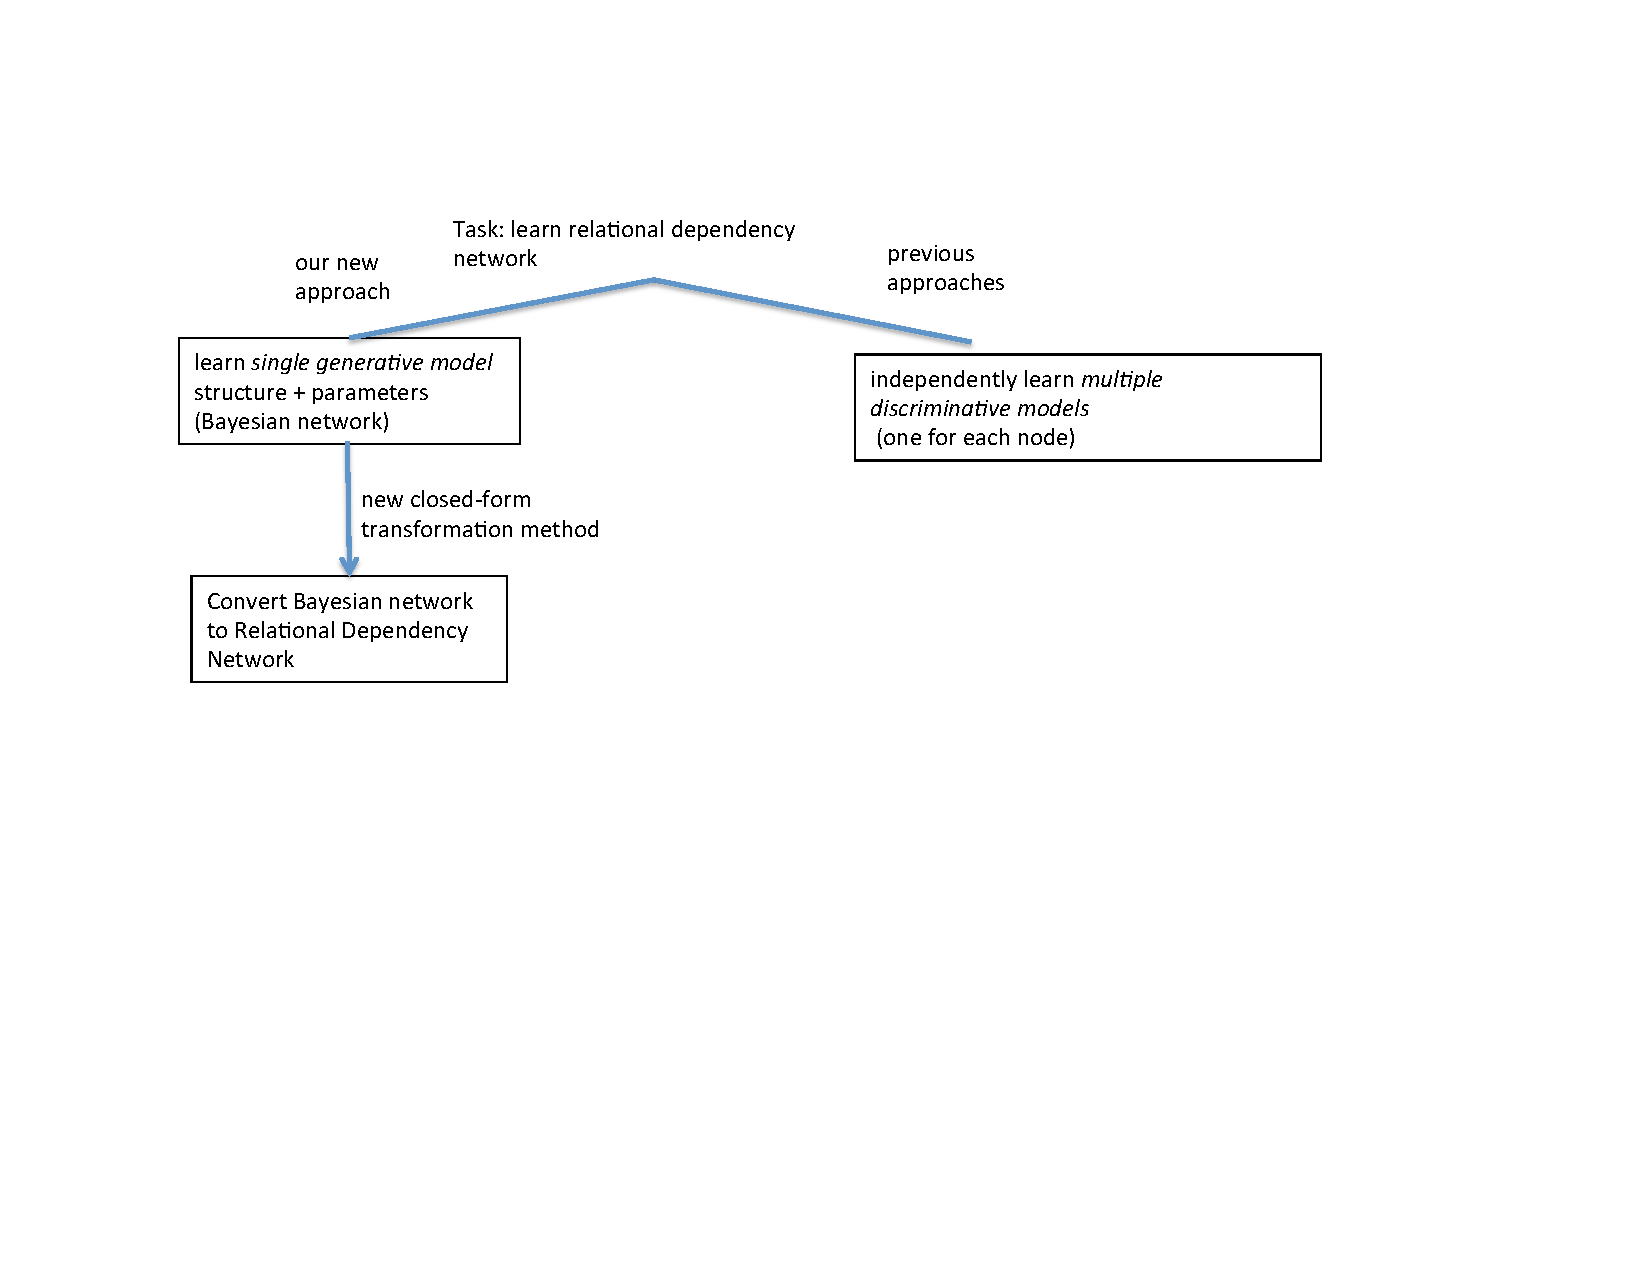
\includegraphics[scale=.45]{novelty.pdf}}
%	\end{minipage}%
%	\begin{minipage}{.75\linewidth}
%		\centering
%		\subfloat[Example of joint and marginal probabilities computed from a toy Bayesian Network structure]{\label{main:b}\includegraphics[scale=.40]{bn.pdf}}
%	\end{minipage}\par\medskip
%	\caption{}
%	\label{fig:propositionalize}
%\end{figure}
%\begin{figure}[!htbp]
%	
%	\begin{minipage}{.5\linewidth}
%		\centering
%		\subfloat[An example database]{\label{main:a}\includegraphics[scale=.6]{databasefigure.pdf}}
%	\end{minipage}%
%	\begin{minipage}{.55\linewidth}
%		\centering
%		\subfloat[The Propositionalization Pipeline]{\label{main:b}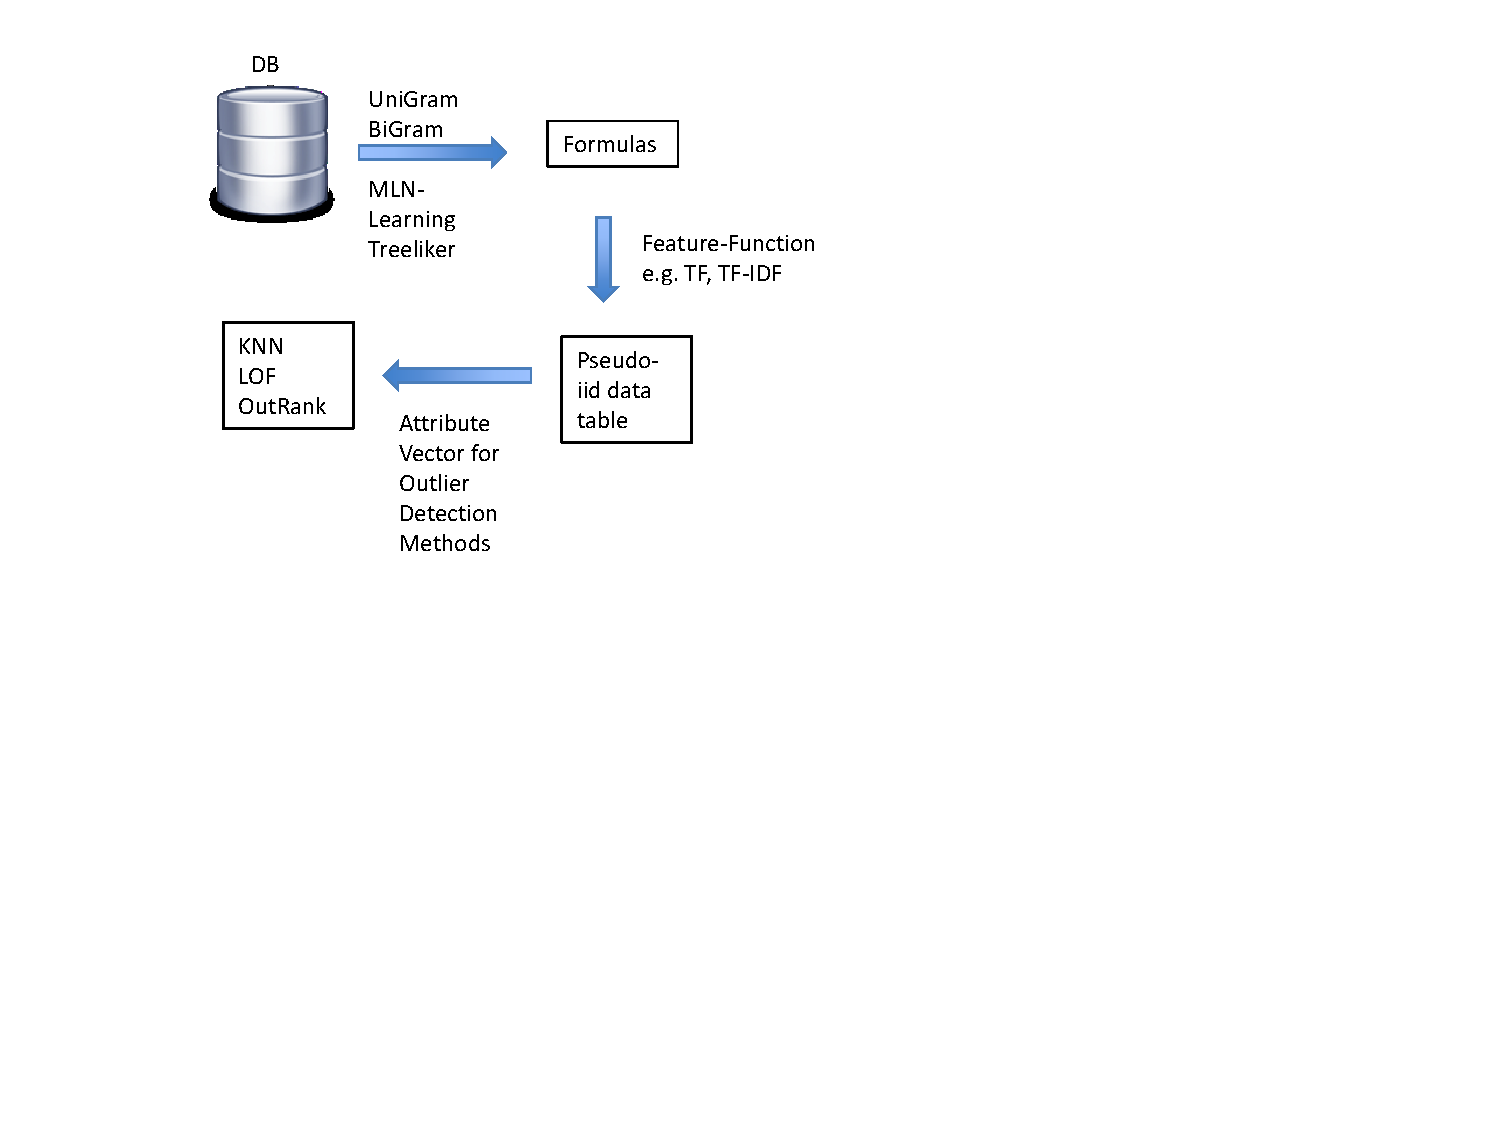
\includegraphics[scale=.45]{pipeline.pdf}}
%	\end{minipage}\par\medskip
%	\caption{System Flow}
%	\label{fig:propositionalize}
%\end{figure}

% We propose new methods for extending statistical  outlier detection to the case of object-relational data using a novel likelihood-ratio comparison for probabilistic models. 
%\paragraph{Markov Logic Network}~\cite{Domingos07} are one of the most well known methods of statistical relational learning. Essentially an MLN consists of a set of weighted first-order formulas that definesa Markov network comprising ground instances of logical predicates. The formulas are the structure of the network and represent associations between ground facts. The weights are the parameters of quantitative components and assign a likelihood to a given relational database by using the log-linear formalism of Markov networks. 
%
% 		\begin{table} 
% 			\caption{Example of a small MLN}
% 			\centering
% 			\resizebox{0.9\textwidth}{!}{
% 				\begin{tabular}{|c|c|l|}
% 					\hline
% 				First-order logic formula&Weight&Translation\\\hline
% 				$\forall(shotEfficiency(p)\rightarrow dribbleEfficiency(p))$&$w_{1}$&
% 					\begin{tabular}{p{3cm}} if shot efficiency of the player is high\\, dribble efficiency is high \end{tabular}\\\hline
% 					
% 					%Synthetic&40&280\\ \hline
% 				\end{tabular}}
% 			\end{table}
 \subsection{Approach}
 Many outlier detection methods have been developed for data that are represented in a propositional format (i.e., as a flat feature vector) or unstructured data.
 
 	\begin{figure*}[!h]
 		\centering
 		\resizebox{1\textwidth}{!}{
 			\includegraphics%[width=0.3\textwidth] 
 			{figures/MLN-Oct13.pdf}
 		}
 		\caption{Categorization of outlier detection methods. The bold font indicates where our methods stand in this categorization.
 			\label{fig:relatedWork}}
 	\end{figure*}
 In a propositional data table, a row represents a data point,
 a column represents an attribute of a data point, and a table entry represents
 an attribute value for a data point.\\
 This dissertation extends unsupervised statistical outlier detection to the case of structured data, more specifically object-relational data. Object-relational data represents a complex heterogeneous network~\cite{Gao2010}, which comprises objects of different types, links among these objects, also of different types, and attributes of these links. Given the prevalence of object-relational data in organizations, outlier detection for such data is an important problem in practice.
 However, applying standard outlier detection methods designed for single data tables on object-relational data runs into impedance mismatch, since object-relational data are represented in multiple interrelated tables.  
 
 In order to detect outliers in object-relational data, we have developed two generative model-based approaches. The advantages of employing a model-based approach for outlier detection task are as follows: 1) We can apply many statistical relational learning methods for building the model. 2) We can leverage statistical concepts such as divergence metrics to measure outlierness of the data points. 3) We can employ outlier detection methods designed for the propositional data.\\
  Based on Figure~\ref{fig:relatedWork} categorization, our proposed outlier detection methods fall into the category of unsupervised, relational learning-based, attributed models which can be applied to both static and dynamic datasets.

 \begin{enumerate}
 	\item In chapter~\ref{chap:four} a model-based method has been proposed to generate conjunctive features for outlier detection task. This method leverages outlier detection tools that are designed for the single table via a pipeline data preprocessing approach by converting the object-relational data into a single attribute-value table, then applying the data analysis tools. Since the attribute value representation corresponds to propositional logic, the conversion is called propositionalization. Propositionalization has been used to detect outliers in the literature. For example, a technique called ODDBALL introduced by Akoglue {\em et al.} extracts graph-centric features to detect anomalies in graph structure~\cite{Akoglu2010}. However, to the best of our knowledge, our work is the first model-based propositionalization approach for outlier detection. In chapter~\ref{chap:four} we show that conjunctive features for outlier detection can be learned from data by using statistical-relational methods. Specifically, we apply
 	Markov Logic Network structure learning method to construct the features. 
 	%
 	%Alternative propositionalization methods that we evaluate in this paper are based on enumerating all conjunctive formulas with at most two literals (unigrams and bigrams). 
 	Compared to baseline propositionalization methods, Markov Logic propositionalization produces the most compact data tables, whose attributes capture the most complex relational correlations. 
 	%(More complex correlations are represented by longer logical formulas). 
 	We apply three representative outlier detection methods ($\lof$, $\knn$, $\outrank$) to the data tables constructed by %Markov Logic 
 	propositionalization.\\
 	This research was published in the proceedings of the Florida Artificial Intelligence Association (FLAIRS2016) conference~\cite{Riahi2016}. 
 	\item Chapter~\ref{chap:five} introduces a model-based method to define outlierness metric. We first apply state-of-the-art probabilistic modelling techniques for object-relational data that construct a graphical model (Bayesian network), which compactly represents probabilistic associations in the data. We propose a new  metric, based on the learned object-relational model, that quantifies the extent to which the individual association pattern of a potential outlier deviates from that of the whole population. The metric is based on the {\em likelihood ratio} of two parameter vectors: One that represents the population associations, and another that represents the individual associations. 
 	Our method is validated on synthetic datasets and on real-world datasets about soccer matches and movies. Compared to the baseline methods, our novel likelihood-based model achieved the best detection accuracy on all datasets except one.
 	
 	Model-based methods have been previously used for outlier detection tasks. Loglikelihood has been used to identify outliers~\cite{Cansado2008}. Rule mining and sub-group mining are another examples of model-based outlier detection~\cite{Agrawal1994, Koh2005}. However, none of these methods are based on a joint distribution distance metric.
 	
 		This work was published in the proceedings of IEEE Symposium series on Computational Intelligence (SSCI 2015) conference and won the best student paper award~\cite{Riahi2015}.
 	
 	In chapter~\ref{chap:six} we compare the log-likelihood distance to metrics of success for a given domain. Success rankings are one of the most interesting features to users. Our reasoning is that high success is an independent metric that indicates an unusual individual. So a correlation between log-likelihood distance and success is an independent validation of the log-likelihood distance, and also shows that this metric points to meaningful and interesting outliers. A version of this work was submitted to the Journal of Data mining and Knowledge discovery.
 \end{enumerate}
   	Figure~\ref{fig:chap1-novelty} provides a tree picture of where our methods are situated with respect to other outlier detection methods and other data models.
   	
   		\begin{figure}
   			\centering
   			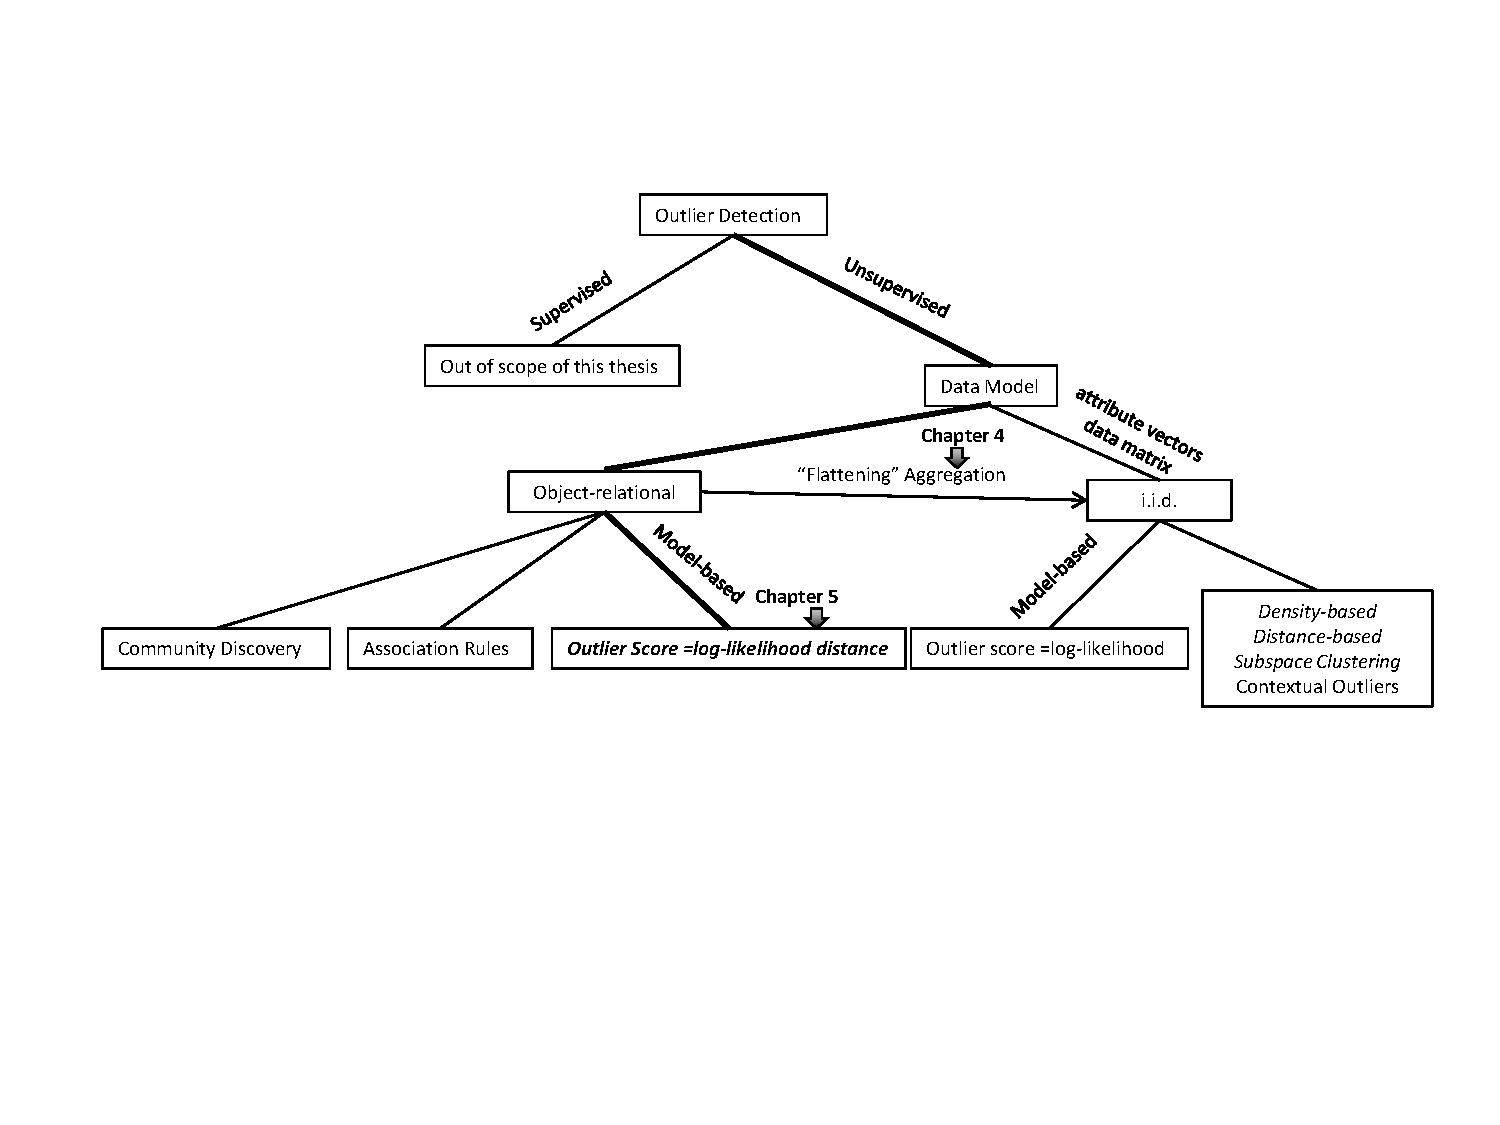
\includegraphics[width=1\textwidth] {figures/all-figures-chapter4-5.pdf}
   			\caption{A tree structure for research on outlier detection for structured data. A path specifies an outlier detection problem, the leaves list major approaches to the problem.
   				\label{fig:chap1-novelty}}
   		\end{figure} 
% In order to tackle the problem of outlier detection for the case of object-relational data, one possible approach is to leverage outlier detection tools that are designed for the single table via a pipeline data preprocessing approach: first, convert the multi-relational data into a single attribute-value table, then apply  the data analysis tools. Since the attribute value representation corresponds to propositional logic, the conversion is called propositionalization.
% %This can be done by to using Markov Logic Network (MLN) structure learning to learn set of formulas from the object-relatinal data and then use these formulas to construct the attributes of the single data table .
% Another possible approach is to apply probabilistic modeling techniques for object-relational data to construct a graphical model that represents normal behavior. An individual is deemed an outlier if the model assigns sufficiently low likelihood to generating its features.
 
%In this dissertation, we address three closely related research problems.
%\begin{enumerate}
%	 \item In Chapter~\ref{chap:four}, We develop a novel propositionalization  approach to unsupervised outlier detection for multi-relational data. Propositionalization summarizes the information from multi-relational data, that are typically stored in multiple tables, in a single data table. The columns in the data table represent conjunctive relational features that are learned from the data. An advantage of propositionalization is that it facilitates applying the many previous outlier detection methods that were designed for single-table data. 
%	 %		Previous work employed propositionalization for classification; in this paper we develop propositionalization for outlier detection. 
%	 We show that conjunctive features for outlier detection can be learned from data using statistical-relational methods. Specifically, we apply
%	 Markov Logic Network structure learning. 
%	 %
%	 %Alternative propositionalization methods that we evaluate in this paper are based on enumerating all conjunctive formulas with at most two literals (unigrams and bigrams). 
%	 Compared to baseline propositionalization methods, Markov Logic propositionalization produces the most compact data tables, whose attributes capture the most complex multi-relational correlations. 
%	 %(More complex correlations are represented by longer logical formulas). 
%	 We apply three representative outlier detection methods ($\lof$, $\knn$, $\outrank$) to the data tables constructed by %Markov Logic 
%	 propositionalization.\\
%	  A preliminary version of this research was published in the proceedings of the Florida Artificial Intelligence Association(FLAIRS2016) conference~\cite{Riahi2016}. 
%	 we use Markov Logic Network (MLN) structure learning to construct a single /data table from multi-relational data. This is a novel application of MLN learning. The format of the resulting data table is an individual-centric representation~\cite{Lippi2011,Lavrac13}:  we assume that there is a target class of individuals to be ranked as potential outliers (e.g. soccer players or movies). A row in the data table represents attributes of an individual. Attributes are defined by logical first-order formulas~\cite{Lippi2011}. The more complex the formula, the more relational information are represented by the formula. 
%	 %A function maps an individual and a first-order formula to a real value that is the value of the attribute for the individual. For example, we use the number of instantiations or groundings of a formula as such a function. 
%	 %
%	 A Markov Logic Network structure is a set of formulas.  Our Markov Logic propositionalization method applies a previous MLN structure learning method to produce a set of formulas; these formulas define attributes for propositionalization. Our approach can be summarized by the equation
%	 
%	 \begin{quote}
%	 	Markov Logic Network Structure = Set of Formulas = Set of Attributes.
%	 \end{quote}
%	 
%	 A baseline comparison method is to enumerate all conjunctive formulas up to a fixed length $n$ as attributes for propositionalization.  This is an instance of the recent Wordification approach to propositionalization \cite{Lavrac13}. A preliminary version of this research was published in the proceedings of the Florida Artificial Intelligence Association(FLAIRS2016) conference~\cite{Riahi2016}. 
	 %	 \item Chapter 5 focuses on the applications of the outlier metric introduced in Chapter 3. One of the important application is to use it in order to rank the individuals. In the datasets used in this dissertation, results show strong correlations between the outlier metric and the success metrics that naturally exists in the data (e.g. salary of the players or standing of the team).
%	\item In chapter 4, we present a new statistical approach to unsupervised outlier detection. 
%	 An individual object is deemed an outlier if  the model assigns sufficiently low likelihood to generating it. 
%	 A class-model Bayesian network (BN) structure is learned with data for the entire population. The nodes in the BN represent attributes for links, of multiple types, and attributes of objects, also of multiple types. To learn the BN model, we apply techniques from statistical-relational learning, a  recent field that combines AI and machine learning \cite{SRL2007,Schulte2012,Domingos2009}. 
%	 The BN provides dimensionality reduction, in the sense that it leverages independencies to represent the data distribution with exponentially fewer parameters than a non-factorized parametrization. 
%	 Given a set of parameter values and an input database, it is possible to compute a {\em class model likelihood} that quantifies how well the BN fits the object data. The class model likelihood uses BN parameter values {\em estimated from the entire class data.} This  is a relational extension of the standard log-likelihood method for i.i.d. vectorial data, which uses the likelihood of a data point as its outlier score. %This can be adapted for object-relational data as follows.
%	 %The Bayes net structure represents the normal pattern of associations among links and attributes  by the well-known d-separation criterion: Two nodes are probabilistically independent if they are d-separated. 
%	 While the class model likelihood is a good baseline score, it can be improved by comparing it to {\em the object model likelihood}, which uses BN parameter values {\em estimated from the object data.}
%	 The {\em model log-likelihood ratio} (LR) is the log-ratio of the object model likelihood to the class model likelihood. This ratio quantifies how the probabilistic associations that hold in the general population deviate from the associations in the object data substructure.
%	 While the 
%	 likelihood ratio discriminates relational outliers better than the class model likelihood alone, it can be improved further by applying two transformations: (1) a mutual information decomposition, and (2) replacing log-likelihood differences by log-likelihood distances. We refer to the resulting novel score as the {\em log-likelihood distance}.	 %For example, for each soccer team, there is a team distribution over: the team's attributes, the team's results in matches, and the actions of the team's players in matches. 
%%	 Step 2: Given a set of object profiles, compute an outlier score that measures how the object's profile differs from the profiles of other objects in its class. We develop a probabilistic approach where:
%	 
%%	 \begin{quote}
%%	 	Object Outlier Score = Score between object distribution and class distribution
%%	 \end{quote}
%%	 
%%	 For each object, the object distribution is a joint distribution over the object's attributes and the attributes of related objects. The object distribution can be computed from counts in the object profile. The class distribution is the distribution of a randomly chosen object in the class. 
%	A preliminary version of this work was published in the proceedings of IEEE Symposium series on Computational Intelligence (SSCI 2015) conference and won the best student paper award~\cite{Riahi2015}. Later on, a more detailed version of this paper was submitted to the Journal of Data mining and Knowledge discovery.
%	
%	 \item In chapter 5, We compare the log-likelihood distance to metrics of success for a given domain. Success rankings are one of the most interesting features to users. Our reasoning is that high success is an independent metric that indicates an unusual individual. So a correlation between log-likelihood distance and success is independent validation of the log-likelihood distance, and also shows that it points to meaningful and interesting outliers. A version of this work was submitted to the Journal of Data mining and Knowledge discovery.
%	 
%	 
%%	  we address an interesting problem of estimating individuals abilities. The idea is to compare each individual ability with the whole population. In the case of soccer player, we form the population to be group of defenders or midfielders or strikers. We used the novel likelihood ratio metric that is introduced in Chapter 4 to quantify the extent to which the individual associate pattern deviates from that of whole population. In order to compute the likelihood ratio metric, we learned two models, A graphical model that represents the population associations pattern and another graphical model that represents the individual association pattern. We use meaningful and independent metrics
%%	 that are available in the data such as salary of a player and box office of a movie as ground truth in order to validate our estimation. An empirical evaluation on soccer and movie data shows a strong correlation between the likelihood ratio and success metric.
%\end{enumerate}

\subsection{Contributions}
The main contributions of this dissertation are the followings:
\begin{enumerate} 
	\item The first approach to outlier detection for structured data that is based on a probabilistic model. 
	\item A new model-based outlier score based on a novel model likelihood comparison, the log-likelihood distance.  % \footnote{Commented paper organization}
	\item A novel task for relational learning: MLN-propositionalization for outlier detection. This facilitates leveraging standard single-table outlier analysis methods for object-relational data.  This task is also a novel application of Markov Logic Network structure learning.
	\item  A novel task for relational learning: propositionalization for outlier detection. This facilitates leveraging standard single-table outlier analysis methods for object-relational data. We use Markove Logic Network (MLN) structure learning for propositionalization task. This is a novel application of MLN structure learning.
	
%	\item A novel application of Markov Logic Network structure learning to perform this task. MLN structure learning learns a compact yet expressive set of features from multi-relational data.
%	\item Our proposed methods rank potential outliers, but do not set a threshold for a binary identification of outlier vs. non-outlier.
\end{enumerate}
\subsection{Limitations and Directions for Future Work}
The main limitations of the work presented in this dissertation are the following:
\begin{enumerate}
	\item \textbf{Limitation of Approach:} 
	\begin{enumerate}\item Our proposed methods rank potential outliers, but do not set a threshold for a binary identification of outlier vs. non-outlier.
		 \item Our current Bayesian Network Learning method can only be applied to discrete data. Prior to learning the model, we take an extra step in data preprocessing and convert the continuous data into discrete which naturally causes some information loss. \item Our generative model-based methods learn a generic Bayesian network structure for the entire population, ignoring the subgroups that inherently exist in the real datasets, as a result, the detected outliers are global outliers. However, there are  more complex outliers that locally deviate from their subgroups and can be detected only by subgroup comparison. One direction for future work is to first detect subgroups in the population and then perform the outlier detection task.
%		 \item In our 
		\end{enumerate}
		\item \textbf{Limitation of Data Analysis: }
	
		In this dissertation, to simplify the outlier detection task, we used only part of the full information available in our rich datasets. The model-based outlier detection can be extended in future work to take advantage of the full information. 
			\begin{enumerate}
				\item In the Premier League dataset, players are naturally related to one another and modelling the interaction between players can be another way to detect anomalous players.
				The graph-based features, such as detecting near-clique nodes and star nodes, proved to be efficient in discovering patterns for anomaly detection task as shown in ODDBALL~\cite{Akoglu2010}.
					\item In this dissertation we did not use the temporal information available in the data. In the learning process we do not give a higher weight (importance) to the more recent action (performance) of an individual. This point is especially important when applying the methods to dynamic data or the data that are collected from long periods of time. 
			\end{enumerate}
		
		%However, this is not a limitation of our proposed outlier detection system.


	%	\item \textbf{Limitation of application: }
	%	\item {local vs global}
	%		\item In this dissertation, we only focus on the action of each individual. In learning the graphical model, we do not take into account the inter-dependencies that inherently exist between individuals for the same class. For example, in the Premier League dataset, players are naturally related to one another and modeling the interaction between players can be another way to detect anomalous players.
%	The connectivity-based features proved to be efficient in discovering patterns for anomaly detection task as shown in ODDBALL.~\cite{Akoglu2010}. %features related to extent of interaction between players are examples of such features in our datasets.
	%one useful piece of information that can be utilized in the future work is to model different groups of individuals to identify which ones usually perform best together.
%	 the information of which players usually work the best together or the other way. 

%	\item Our current Baysian Network Learning model can only be applied to discrete data. Prior to learning the model, we take an extra step in data preprocessing and convert the continuous data into discrete which naturally causes some information loss. 
%	\item In this dissertation we assume the structure of the learned Bayesian network is fixed and we learned the parameters for that fixed structure. 
%	\item In our learning process, we do not give a higher weight (importance) to the more recent action (performance) of an individual. This point is especially important when applying the methods to dynamic data or the data that are collected from long periods of time. 
%	\item We do not leverage domain knowledge in our modelling. There are some attributes that play more important roles in evaluating individuals of a specific class. For example in Soccer domain, the shot efficiency or number of goals scored by a strikers is more important compare to other attributes such as the dribble efficiency.
\end{enumerate}
%-dynamic nist , we didnt weight the recent history more than old ones. -action between two players



 
%% Copyright 1998 Pepe Kubon
%%
%% `two.tex' --- 2nd chapter for thes-full.tex, thes-short-tex from
%%               the `csthesis' bundle
%%
%% You are allowed to distribute this file together with all files
%% mentioned in READ.ME.
%%
%% You are not allowed to modify its contents.
%%

%%%%%%%%%%%%%%%%%%%%%%%%%%%%%%%%%%%%%%%%%%%%%%%%%
%
%     Chapter 2   
%
%%%%%%%%%%%%%%%%%%%%%%%%%%%%%%%%%%%%%%%%%%%%%%%%

\chapter{Literature Review}
\label{chap:two}
This chapter provides a literature review of the state-of-the-art methods in the field of outlier detection. 
%In Section \ref{sec:outdefinition}, we formally define outlier, different types of outlier and the applications of outlier detection. 
Outlier detection is a very well-explored area and there are many surveys to overview the state-of-the-art methods. Each survey categorized these methods differently. The categorization can be based on datatype (e.g. graph data) or type of methods that have been used to detect outliers (e.g. structured-based methods). In this chapter we group outlier methods based on the format of the input data, whether it is presented in a single data table or it has a higher level of organization such as data presented in a relational database, or XML format or OLAP. Since the focus of our work is on the structured data, we mainly concentrate on the methods designed for that data format .\\% We further categorized each type into supervised and unsupervised approaches. 
%Different surveys categorized outlier detection work In Section \ref{sec:categorizedMethods}, we categorized different outlier detection techniques into supervised and unsupervised and briefly discuss some methods of each category.
% Since the focus of this dissertation is on outlier detection for Object-relational data, we devote the entire Section \ref{sec:outlierinSRL} to explore relational-based outlier detection methods. 
 We conclude this chapter with section \ref{sec:limitaion} which addresses the limitations of current outlier detection methods. Figure~\ref{fig:categorization} shows the organization of this chapter.
	\begin{figure*}[!htbp]
		\centering
		\resizebox{0.8\textwidth}{!}{
			\includegraphics%[width=0.3\textwidth] 
			{figures/chapt2Category.pdf}
		}
		\caption{ Related work categorization
			\label{fig:categorization}}
	\end{figure*}
%\section{Background and Notation \label{sec:background}}
%In this section, we introduce some	notation and terminology that is referred to throughout this dissertation. We present a brief discussion on probability, Bayesian networks and Markov Logic Network. Please refer to the citations to find more information for any of the discussed topics.
%
%\subsection{Probability Distribution}
% Throughout this dissertation, \textbf{random variables} are denoted by  by capital letters (X,Y,...) and the values of a random variable by lower case letters (x,y,...).  We denote sets of random variables by \textbf{X}=\{$\X_{1},\ldots,\X_{n}$\}. 
%%The \textbf{range} of the variable is the set of values of the variable. In this dissertation we only consider random variables with a \emph{finite range}.
% The notation $P(X_1 = x_1,...,X_n = x_n) = p$, sometimes abbreviated as $P(\x_1,...,\x_n) = p$, or $P(\mathbf{X} = \mathbf{x}) = p$ means that the \textbf{joint probability} of random variables $X_{1},\ldots,X_{n}$ taking on values $\x_1,\dots,\x_n$ is $p$. 
% 
%By the laws of probability the sum of the joint probability distribution of a set of random variables $\textbf{\X}$ over all possible values $\textbf{x}$ is 1, that is,
%
%$$\sum_\textbf{x}{ P(\textbf{X} =\textbf{x})}=1 $$  
%
%
%The joint probability distribution of a subset $\textbf{Y}$ of $\textbf{X}$ can be obtained by summing out the remaining variables $\textbf{Z} = \textbf{X} \backslash \textbf{Y}$. The distribution is called the \textbf{marginal probability} distribution of $\textbf{\Y}$ and can be obtained by the following formula:
%
%$$ P(\textbf{Y}) = \sum_{\textbf{z}} P(\textbf{Y}, \textbf{Z} = \textbf{z}) $$
%
%Given as subset  $\textbf{Z} \in \textbf(Z)$, the \textbf{conditional probability} of a subset  $\textbf(Y) \in \textbf(X)$ can be derived from the following formula:
%$$ P(\textbf{Y}| \textbf{Z}) = \frac{P(\textbf{Y}, \textbf{Z})}{P(\textbf{Z})}$$
%
%%The conditional probability of a subset $\textbf(Y) \in \textbf(X)$ given a subset $\textbf{Z} \in \textbf(Z)$ is the probability of  $\textbf{Y}$ occurring when we know $\textbf{Z}$ has occurred. The \textbf{conditional probability} can be obtained by the following formula:
%%
% \emph{Independent} events are events that occurrence of one event does not effect the other. The joint probability of the two independent  events is the product of each event occurrence. 
%%
%%Two events $\textbf{X}$ and $\textbf{Y}$ are \emph{independent} if occurrence of  $\textbf{X}$ does not effect the probability of $\textbf{Y}$ occurring. In such a event, the joint probability of the two events co-occurring is calculated by the product of each of their occurrence:
%
%$$ P(\textbf{X}, \textbf{Y}) = P(\textbf{X}) \times P(\textbf{Y})$$
%
%\subsection{Predicate Language}
%
%We employ the notation of Chiang and Poole \cite{Chiang2012} for logical syntax, as follows.
%%
%Constants are expressed in lower-case, e.g. $\it{joe}$, and are used to represent individuals. A type is associated with each individual, e.g. $\it{joe}$ is a person. We use $D(\tau)$ to represent a domain of type $\tau$, which is the set of individuals of type $\tau$. A {\em logical variable} is written in upper case. A logical variable is also typed, e.g. $\it{Person}$ denotes some member of $D(\tau)$. A relation is given by 
%$$r : \Omega \rightarrow V_{r}$$
%where $r$ is the name of the relation, $\Omega_{r}=D(\tau_{1})\times \ldots \times D(\tau_{a})$ is the domain of the relation, and $T_{r}=(\tau_{1},\ldots,\tau_{a})$ is the type of the relation. $V_{r}={v_{1},\ldots,v_{k}}$ is the range of the relation. Number $a$ and $k$ are positive integers denoting the {\em arity} and {\em size} of $r$. An {\em atom} is an expression of the form $r(\sigma_{1},\ldots,\sigma_{a})$ where each $\sigma_{i}$ is either a constant or logical variable. If all of $\sigma_{1},\ldots,\sigma_{a}$ are constants, $r(\sigma_{1},\ldots,\sigma_{a})$ is a {\em ground atom}.
%
%A {\em literal} specifies the value of an atom e.g. $r(X_{1},\ldots,X_{a})=v$ where $v \in V_{r}$. A literal is also a {\em formula}. Formula with multiple literals are formed using connectives $\wedge$ and or $\vee$. Connecting literals using only $\wedge$ forms a {\em conjunctive formula } or {\em conjunction}. A formula that contains no logical variables is a {\em ground} formula.
%%, is a proposition.
%%A {\em disjunctive formula} or {\em disjunction} is formed using only $\vee$. \\
%
%A substitution is a set $\{X_{1} \textbackslash x_{1}, \ldots, X_{k}\textbackslash x_{k}\}$ where $X_{i}$ are distinct logical variables and $x_{i}$ are constants. When applied to a formula $f$, each occurrence of $X_{i}$ in $f$ is replaced with $x_{i}$. We denote the application of a substitution 
%%$\{X_{1} \textbackslash x_{1}, \ldots, X_{k}\textbackslash x_{k}\}$ 
%to $f$ as $f\{X_{1} \textbackslash x_{1}, \ldots, X_{k}\textbackslash x_{k}\}$. 
%Consider a formula $f$ containing logical variables $X_{1}, \ldots,X_{n}$, where each $X_{i}$ has type $\tau_{i}$. The {\em grounding space} of $f$, is the set of all possible grounding substitutions for $f$, given by 
%$$\{\{X_{1}\textbackslash x_{1}, \ldots, X_{n}\textbackslash x_{n}\}:x_{i} \in D(\tau_{i}) \mbox{ for } i=1,\ldots,n\}.$$
%
%%	Given some formula $f$ containing logical variables $X_{1}, \ldots,X_{n}$, where each $X_{i}$ has type $\tau_{i}$, let the domain of $f$ be $\Omega_{f}=D(\tau_{i}\times \tau_{n})$. The {\em substitution space} of $f$, $\Gamma_{f}$, is the set of all possible grounding substitutions for $f$, given by 
%%	$$\Gamma_{f}=\{\{X_{1}\textbackslash x_{1}, \ldots, X_{n}\textbackslash x_{n}\}:(x_{1},\ldots,x_{n})\in \Omega_{f}\}.$$
%
%A \emph{database} $\D$ specifies for each ground literal whether the literal is true in the database or not. A ground conjunction is true in a database if all of its conjuncts are true. The \emph{count} of groundings satisfying formula $\formula$ with respect to a database $\D$ is denoted as $\grounds_{\D}(\formula)$.
%
%\subsubsection{Examples} Figure~\ref{fig:exampledatabase} shows an example database. The ground literal $$(\it{ShotEff(\P,\M)} = Low) \{\P\textbackslash 123,\M\textbackslash 1\}=(\it{ShotEff}(123,1)=Low)$$ evaluates as true in this database. For the grounding count we have $$\grounds_{\D}(\it{ShotEff(\P,\M)} = Low) \{\P\textbackslash 123\}) = 2.$$
%
%
%
%\begin{figure*}[htbp]
%	\centering
%	\includegraphics[width=0.5\textwidth]{figures/databasefigure.pdf}
%	\caption{An example database
%		\label{fig:exampledatabase}}
%\end{figure*}
%\subsection{Bayesian Networks} \label{Sec:BayesianNetwork}
%A {\bf Bayesian Network (BN)} is a directed acyclic graph (DAG) whose nodes comprise a set of random variables \cite{Pearl1988}. Depending on context, we interchangeably refer to the nodes  and variables of a BN. Fix a set of variables $\Features = \{\feature_{1},\ldots,\feature_{n}\}$. 
%%These are attributes of objects, which can and typically do belong to different classes. In statistical terms, each attribute defines a random variable. 
%The possible values of $\feature_{i}$ are enumerated as $\{\nodevalue_{i1},\ldots,\nodevalue_{i\states_{i}}\}$. The notation $P(\feature_{i} = \nodevalue)\equiv P(\nodevalue)$ denotes the probability of variable $\feature_{i}$ taking on value $\nodevalue$. We also use the vector notation $P(\Features = \set{\nodevalue}) \equiv P(\set{\nodevalue})$ to denote the joint probability that each variable $\feature_{i}$ takes on value $\set{\nodevalue}_{i}$. 
%
%
%The conditional probability parameters of a Bayesian network specify the distribution of a child node given an assignment of values to its parent node. For an assignment of values to its nodes, a BN defines the joint probability as the product of the conditional probability of the child given its parent values, for each child node in the network. This means that the log-joint probability can be {\em decomposed} as the node-wise sum
%
%\begin{equation} \label{eq:bn}
%\ln P(\Features = \set{\nodevalue};\model,\parameters) = \sum_{i=1}^{n} \ln \parameter(\set{\nodevalue}_{i}|\set{\nodevalue}_{\parents_{i}})
%\end{equation}
%
%where $\set{\nodevalue}_{i}$ resp. $\set{\nodevalue}_{\parents_{i}}$ is the assignment of values to node $i$ resp. the parents of $i$ determined by the assignment $\set{\nodevalue}$. 
%%The function $\ln$ is the binary logarithm base 2. 
%To avoid difficulties with $\ln(0)$, here and below we assume that joint distributions are positive everywhere. Since the parameter values for a Bayes net define a joint distribution over its nodes, they therefore entail a marginal, or unconditional, probability for a single node. We denote the \textbf{marginal probability} that node $\feature$ has value $\nodevalue$ as $P(\feature = \nodevalue;\model,\parameters) \equiv \parameter(\nodevalue)$.
%
%\paragraph{Example.} Figure~\ref{fig:BayesNet} shows an example of a Bayesian network and associated joint and marginal probabilities.
%\begin{figure} %  figure placement: here, top, bottom, or page
%	\centering
%	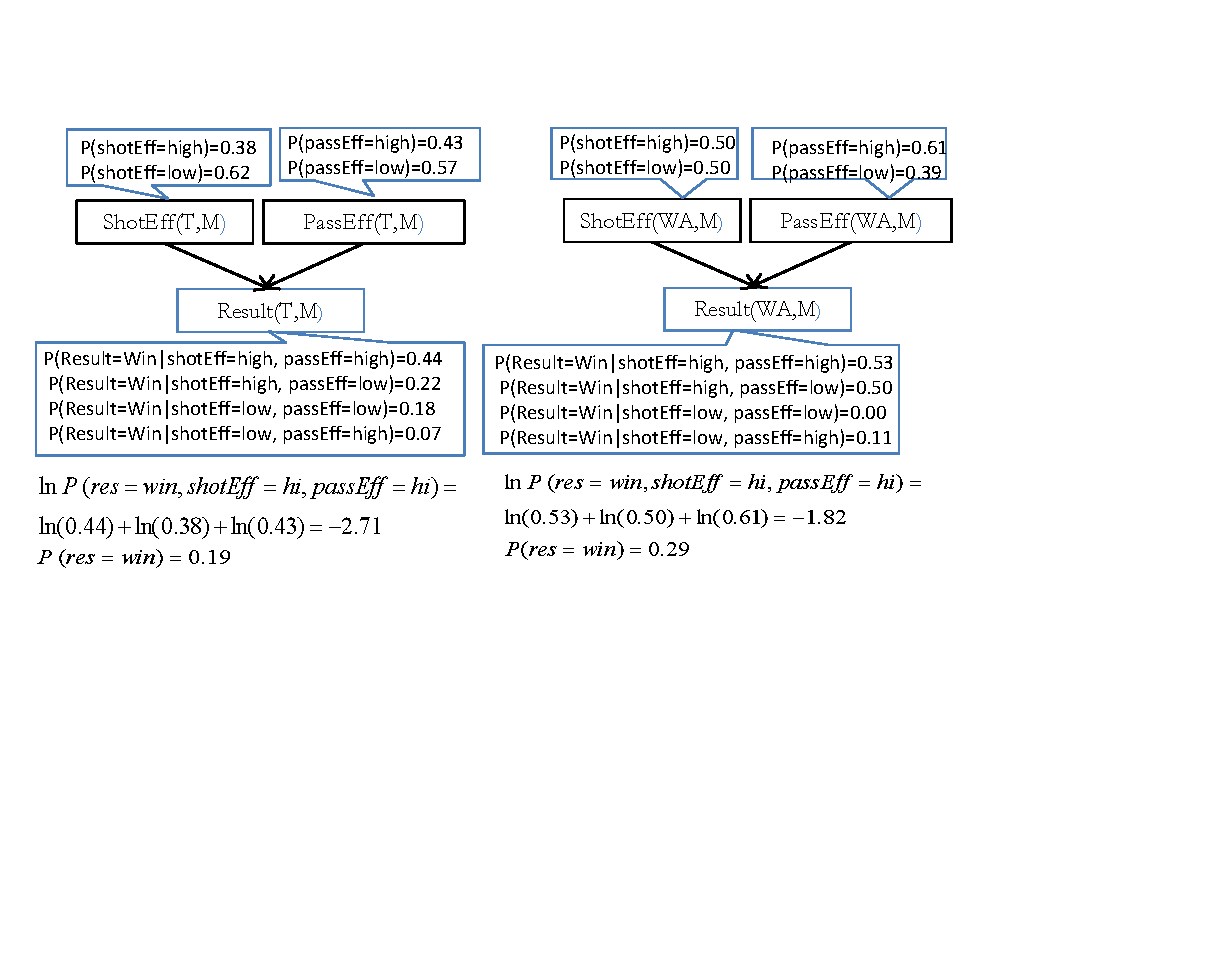
\includegraphics[width=0.9\textwidth]{figures/bnuncropped} 
%	\caption [An example of a Bayesian network ]{ Example of joint and marginal probabilities computed from a toy Bayesian Network structure \label{fig:BayesNet}}
%\end{figure}
%\subsubsection{Learning Bayesian Networks} \label{Sec:learningBN}
%The goal of structure learning is to find a directed acyclic graph $G$ that represents a set of variables $V$ and a dataset $\mathcal{D}$ containing independent and identically distributed (i.i.d) examples from an unknown distribution $P$. For every possible edge in the network structure leaning algorithm must determine whether to include that in the final network or not. The total possible number of graphs is super exponential in $|V|$. Even restricting the domain and constraining variables to have at most $k$ parents has been proven to be NP-Complete.
%\subsubsection{Markov Logic Network} \label{Sec:MLNIntro}
%Markov Logic Network~\cite{Domingos07} 
%is one of the most well known methods of statistical relational learning. Essentially an MLN consists of a set of weighted first-order formulas that defines a Markov network comprising ground instances of logical predicates. The formulas are the structure of the network and represent associations between ground facts. The weights are the parameters of quantitative components and assign a likelihood to a given relational database by using the log-linear formalism of Markov networks. Table~\ref{MLNSample} shows an MLN for the Soccer domain.
%
%%\begin{table} 
%%	\caption{Example of a small MLN}
%%	\centering
%%	\resizebox{0.9\textwidth}{!}{
%%		\begin{tabular}{|c|c|l|}
%%			\hline
%%			First-order logic formula&Weight&Translation\\\hline
%%			$\forall(shotEfficiency(p)\rightarrow dribbleEfficiency(p))$&$w_{1}$&
%%			\begin{tabular}{p{3cm}} if shot efficiency of the player is high\\, dribble efficiency is high \end{tabular}\\\hline
%%			
%%			%Synthetic&40&280\\ \hline
%%		\end{tabular}}\label{MLNSample}
%%	\end{table}
%\begin{table}
%	\centering
%	\begin{tabular}
%		{|l|l|l|} \hline
%		First-order logic  & Weight& English \\ \hline
%		\multirow{2}{*} {$\forall x (shotEfficiency(x) \Rightarrow dribbleEfficiency(x))  $} & \multirow{2}{*} {$w_1$} & if shot efficiency of the player is \\ & &high then  dribble efficiency is high \\ \hline
%%		$\forall x \forall y (intelligent(x) \wedge  friend(x,y)$ & \multirow{2}{*}{ 0.7}& If a student has an intelligent \\ $\Rightarrow$ $intelligent(y)$) & & friend then he is intelligent  \\ \hline
%	\end{tabular}
%	\caption{Example of a small MLN }
%	\label{MLNSample}
%\end{table}
%Given a set of variables $V$ and a dataset $\mathcal{D}$ containing independent and identically distributed (i.i.d) examples from an unknown distribution $P$, the goal of structure learning is to identify a directed acyclic graph $G$ that represents $P$.
% Finding an optimal structure is a computationally intractable problem; structure learning algorithms determine for every possible edge in the network whether or not to include the edge in the final network and which direction to orient the edge. The total possible number of graphs is super exponential in $|V|$. Even a restricted form of structure learning where variables are constrained to have at most $k$ parents has been proven to be NP-Complete.
% Two broad classes of structure learning are well-known in the literature \cite{Neapolitan2004,Heckerman1998}. 
%
%\begin{itemize}
%	\item Score Based methods search over possible Bayesian network structures for the most suitable factorization of the joint probability based on $\mathcal{D}$. The model selection criterion is usually defined as a score that the methods are trying to maximize. BDeu \cite{Heckerman1994} and BIC \cite{Chickering2003} are examples of well known scores for Bayesian network learning.
%	
%	\item Constraint Based methods employ a statistical tests to detect conditional (in)dependencies given a sample $\mathcal{D}$, and then compute a BN structure $G$ that fits the (in)dependencies \cite{Margaritis2000,Cheng2002}. The  (in)dependencies test can be chosen to suit the type of available data and application domain. One of the traditional test for categorical data is the $\chi^2$ test.
%
%\end{itemize}
%
%To form a complete Bayes net, an additional step of parameter estimation is required to determine ${\theta}_G$ from $\mathcal{D}$. Since the focus of this dissertation is on structure learning, techniques for parameter estimation will not be addressed here. (See e.g. \cite{Heckerman1998} for details).

%\subsubsection{Parametrized  Bayes Nets}
%Parametrized Bayes nets(PBNs) were introduced by Poole to study first-order probabilistic inference on directed models. They are a comparatively simple adaptation of the Bayes net format for relational data. The syntax of PBNs is similar to that of other directed graphical SRL models, such as Bayes Logic Programs \cite{Kersting2007} and Probabilistic Graphical Models \cite{Friedman99prm}. A Parametrized Bayes Net structure consists of: (1) a directed acyclic graph whose nodes are functor nodes. (2) a population for each first-order variable. (3) an assignment of a range to each functor. A Parametrized Bayes Net is a Bayes net whose graph is a  parametrized Bayes Net structure. Because each of the nodes in a parametrized Bayes net is a functor, We also use the name Functor Bayes Nets (FBNs) for them. 


%\subsection{Relational Data and Databases} \label{sec:relationaldata}
% We adopt a functor-based notation for combining logical and statistical concepts~\cite{Poole2003,Kimmig2014}.
% A functor is a function or predicate symbol. Each functor has a set of values (constants) called the \textbf{domain} of the functor. The domain of a \textbf{predicate} is $\{\true,\false\}$. Predicates are usually written with uppercase Roman letters, other terms with lowercase letters.
% A predicate of arity at least two is a \textbf{relationship} functor. Relationship functors specify which objects are linked. Other functors represent \textbf{features} or \textbf{attributes} of an object or a tuple of objects (i.e., of a relationship).
% A \textbf{population} is a set of objects. 
% A \textbf{term} is of the form $f(\term_{1},\ldots,\term_{k})$ where $\functor$ is a functor %(either a function symbol or a predicate symbol) 
% and each $\term_{i}$ is a first-order variable or a constant denoting an object. A term is \textbf{ground} if it contains no first-order variables; otherwise it is a first-order term. In the context of a statistical model, we refer to first-order terms as \textbf{Parametrized Random Variables} (PRVs) \cite{Kimmig2014}. 
% %A term whose range are the truth values $\{\true,\false\}$ is a \textbf{predicate}. 
% %Predicates are usually written with uppercase Roman letters, other term with lowercase letters.
% %The grounding concept represents moving from the population-level  to the object level. 
% A \textbf{grounding} replaces each first-order variable in a term by a constant; the result is a ground term. A grounding may be applied simultaneously to a set of terms.  A relational database $\D$ specifies the values of all ground terms, which can be listed in data tables. 
% %In machine learning terminology, the data tables are contingency tables that represent sufficient statistics or event counts.
 
% Consider a joint assignment 
% $P(\Features = \set{\nodevalue})$ of values to a set of PRVs $\Features$. The {\em grounding space} of the PRVs is the set of all possible grounding substitutions, each applied to all PRVs in $\Features$. The {\em count} of groundings that satisfy the assignment with respect to a database $\D$ is denoted by $\grounds_{\D}(\Features = \set{\nodevalue})$. The \textbf{database frequency} $P_{\D}(\Features = \set{\nodevalue})$ is the grounding count divided by the number of all possible groundings.
% 

%\paragraph{Object-relational data}
%\subsection{Object-relational data} \label{Sec:objectRelationl}

\section{Outlier Detection Methods for Propositional Data} \label{sec:categorizedMethods}
In this section we explore outlier detection methods that take \textit{propositional} data. One interpretation of propositional data is that the attributes describe characteristics of one object-class. For example, $\mathit{shotEfficiency(Player)}$ shows shot efficiency of a player in general, while in the structured data the attributes are more complex; for example in the Object-relational data model, the attributes are shown in this format: $\mathit{shotEfficiency(Player, Match})$ which represents shot efficiency of a player in a match and involves two object-classes.   Throughout this dissertation, we call the methods designed for single data table propositional methods. In this section, we further categorize these methods into supervised and unsupervised based on whether the sample of data has been provided with labels and domain expert information to build an outlier detection model.
%\begin{figure*}[!htbp]
%	\centering
%	\resizebox{1\textwidth}{!}{
%		\includegraphics%[width=0.3\textwidth] 
%		{figures/structure.pdf}
%	}
%	\caption{Categorizing outlier detection methods.
%		\label{fig:Overview}}
%\end{figure*}
\subsection{Supervised Methods for Propositional Data}
These methods model both normality and abnormality and requires pre-labelled data. Normal points may belong to a single class or be divided among different classes. Supervised outlier detection is a special case of the classification where the labels are extremely unbalanced in terms of occurrence~\cite{Chawla2004}.
Normal data points are easily available while outlier examples are very sparse and it is the rarity that makes these data points outliers. In this sense, outlier detection can also be viewed as $\it{rare class}$ detection problem. The imbalanced nature of outlier detection makes the accurate classifications quite hard to achieve and it might result in over-training \cite{aggarwal2013}.

When the purpose of classification is outlier detection, cost-sensitive variations of machine learning algorithms can be used in order to make the classification of anomalies more accurate \cite{aggarwal2013}.
Class imbalance is one of the common problems in supervised outlier detection. The standard evaluation techniques in classifications cannot simply be applied to outlier detection. For example, in the case of breast cancer, where 99\% of scans are identified to be normal and only 1\% abnormal, the trivial classification algorithm, which returns all the instances in the test cases as normal, would have a high accuracy of 99\%. However, it is not useful in the context of detecting breast cancer. Cost-sensitive learning is one way that has been used to handle the class imbalance problem in outlier detection. The objective function of the classification in this type of learning has been designed in a way that it weights the errors in classification differently for different classes.  In this case, classifiers are tuned so the errors in classification of outliers are more penalized compared to the misclassified normal classes~\cite{Elkan2001}. In other words, methods are forced to predict the outlier class far better than the normal class. This trade-off is characterized either by the precision-recall curve or a receiver operating characteristics ($ROC$) curve.\\
Active re-sampling is another way to tackle class imbalance problem. The relative proportion of the rare classes is magnified through re-sampling. This approach can be considered as an indirect form of cost-sensitive learning.\\
Classification outlier methods can be grouped into two categories: 
\begin{itemize}
	\item Multi-class: Training data in this group contains the instances from multiple normal classes~\cite{Claudio2000}. First, a classifier is learned to distinguish between instances from different normal classes. If a test instance is not classified as normal by any of the classifiers, then it is labeled as an outlier.
	\item One-class: All training instances belong to a single class label. If any test case does not fall into the normal boundary, it is identified as an outlier. Examples of well-known algorithms are:
	\begin{itemize}
		\item  One-class SVMs \cite{Scholkopf2001}
		\item  One-class Kernel Fisher Discriminant~\cite{Roth2005}
	\end{itemize}
\end{itemize}


In the following subsections, we provide examples of supervised methods in different areas.

%\subsubsection{Naive Baye}
%Naive Bayesian networks for classifications can also be applied to outlier detection. Amor {\em et al.}  uses Naive Bayes in intrusion detection and consider three levels of attack~\cite{Amor2004}: 
%\begin{enumerate}
%	
%	
%	\item Whole attacks where they evaluate the ability of Naive Bayes to detect each elementary attack.
%	\item Group the attacks into four main categories to identify which category a given connection belongs to.
%	\item Focus on normal and abnormal behavior and estimate whether an observation falls into one class or not.
%\end{enumerate}

% \cite{Das2008} focuses on detecting anomalies in categorical datasets.

\subsubsection{Neural Network}
Neural networks are applied to outlier detection in one-class learning as well as multi-class  scenarios. At the first step, a neural network is trained on normal training data in order to learn the normal behavior of data points. Then, test instances are presented to the neural network. If the test is accepted, the data point is normal, otherwise, it is an outlier. Different neural network techniques have been proposed to tackle outlier detection problem. Ghosh {\em et al.} \cite{Ghosh98} apply multi-layered perceptrons and focus on detecting attacks on computer systems. They perform intrusion detection on software programs instead of what most intrusion detection systems do by analyzing network traffic and host system logs. They build a profile of software behaviour to distinguish between a normal software behaviour and a malicious one.

\subsubsection{Support Vector Machine}
Support Vector Machines have been applied to outlier detection mostly in a one-class setting. These techniques first learn a region that includes the training data points. If a test instance falls into the learned region, it is considered as normal, otherwise, it is an outlier~\cite{DavyG02,RatMikSchMul02}.
%\subsubsection{Hidden Markov Model}
%Zhang {\em et al.}~\cite{Zhang2005} designed a semi-supervised hidden markov model framework that learns normal events from labeled samples and unusual events are modeled using Maximum a Posteriori adaptation. By maximizing the likelihood of observation sequences of the normal events, a set of parameters of {\em HMM} models is learned. The probability density function of the learned model is assumed to be Gaussian mixture model. Given this well estimated normal event model, the likelihood of each test data point is computed. 
\subsection{Unsupervised Methods for Propositional Data}
In the datasets where data points are not labeled, unsupervised approaches make some assumptions about the behaviour of outliers. Based on the assumptions made, these methods can be categorized.
\subsubsection{Probabilistic and Statistical Models}
In the probabilistic and statistical model, the data is assumed to be derived from a closed form of probability distribution and the goal is to learn the parameters of this model. Therefore, the main challenge is to choose the data distribution. The parameter of the distribution can be learned by using different algorithms, such as Expectation Maximization. The key output of this method is the membership probability of data points to the distribution; the ones that have a very low fit will be considered as outliers. Extreme Value Test can also determine the outliers in this stage~\cite{aggarwal2013}. 

The most popular statistical modeling is detecting extreme values that determine data values at the tails of a uni-variate distribution. However, these methods were not designed to focus on issues such as data representation or computational efficiency. 
Also, most of the multidimensional outliers cannot be determined through extreme data values and are usually defined by the relative positions of data points with respect to each other. While extreme value analysis may be applicable to only a specific type of data, they have many applications beyond the univariate case since the final step in most outlier detection methods is to identify extreme values to assigned scores. Gao {\em et al.}  have worked on the problem of identifying extreme values from the outlier scores \cite{GaoT06}. 

Laurikkala {\em et al.} describe one of the simplest statistical outlier detection methods where an information box plot has been used to identify outliers in both uni-variate and multivariate datasets~\cite{Laurikkala00}. For multivariate datasets the authors claimed that there is not any clear ordering, but they suggested using reduced sub-ordering based on the generalized distance metric using the \textit{Mahalanobis} distance. Mahalanobis distance is similar to the Euclidean distance, except that it normalizes the data on the basis of the inter-attribute correlation and scales the distance values by local cluster variances along the directions of correlation. Consider a dataset containing $k$ clusters. Assume that the $r$th cluster in $d$-dimensional space has a corresponding $d$-dimensional mean vector $\bar{\mu_{r}}$ and a $d\times d$ co-variance matrix $\Sigma_{r}$. The $(i,j)$th entry of this matrix is the co-variance between dimension $i$ and $j$ in that cluster. Then, the Mahalanobis distance $MB(\bar{X}, \bar{\mu_{r}})$ between a data point $\bar{X}$ and the cluster centroid $\bar{\mu_{r}}$ is as follows: 
\begin{equation}
MB(\bar{X},\bar{\mu_{r}} )=(\bar{X}-\bar{\mu_{r}} )\cdot \Sigma_{r}^{-1}\cdot (\bar{X}-\bar{\mu_{r}} )^T
\end{equation}
Intuitively, this metric scales the square distances by the cluster variances along the different directions of correlation.\\
\subsubsection{Bayesian Network}
In order to detect disease outbreak early, Wong {\em et al.} \cite{Wong2003} compared the distribution of data against a baseline distribution. A different environmental attribute, such as trends caused by the day of a week and by seasonal variations in temperature and weather, makes defining such a baseline hard, if not impossible. By using Bayesian network that takes the joint distribution of the data and conditioning on attributes that are responsible for the trends, they were able to define such a baseline.

Babbar {\em et al.}~\cite{Babbar2010} used joint probability distribution and knowledge of the domain driven by Bayes net to identify low probable data points with intrinsic anomalous patterns and they treat them as potential outliers.

Cansado {\em et al.}~\cite{Cansado2008} followed a probabilistic approach and modeled the joint probability density function of the attributes of data points in the database and ranked the records according to their oddness. They used Bayesian Networks in order to estimate the joint probability density function and handle its complexity, .
\\ 
%In general outliers in probabilistic models can be categorized as: 
%\begin{description}
%	\item [1: Uni-variate outliers] The simplest kind of outliers are uni-variate and can be mostly identified by extreme value analysis where the values which are either too large or too small are considered outliers. The first step is to estimate an underlying distribution for data and then determine the statistical tail of that distribution. Extreme value statistics is different from the traditional outlier detection methods that treat objects based on their generative probabilities rather than their extreme values~\cite{AchtertHKSZ11}.
%	\item [2: Multivariate outliers]
%	To identify outliers in multivariate data extreme value analysis can still be used. Some methods try to model the underlying distribution explicitly and others are based on statistical analysis and do not assume any underlying data distribution. These methods can be further categorized into:
%	\begin{description}
%		\item [Deviation-based methods]In {\em deviation based} methods, the impact of outliers are measured on the variance. Arning {\em et al.}\cite{ArningAR96}  measure how much decrease in the variance of the data can be seen when a particular data point is removed.
%		\item [Angle-based methods] The idea behind {\em angle-based} method is that interior data is more likely to be enclosed by the data points at the boundaries and intermediate points are more likely to have data points around them at different angles. For example, consider the two data points $A$ and $B$ in Figure~\ref{fig:anglebased}, in which point $A$ is an outlier, and point $B$ lies in the interior of the data. All data points lie within a limited angle centred at $A$, on the other hand it is not the case for data point $B$ which lies within the interior of the data.
%		The more isolated the data point the smaller the angle gets. Kriegel {\em et al.} focus on the advantages of angular measure in identifying outliers~\cite{Kriegel2008}.
%		\item [Distance distribution-based methods] {\em distribution dependent} approaches model the entire dataset in normal distribution format about its mean in the form of multivariate Gaussian Distribution. 
%	\end{description}
%	
%	\begin{figure*}[!htbp]
%		\centering
%		\resizebox{0.8\textwidth}{!}{
%			\includegraphics%[width=0.3\textwidth] 
%			{figures/anglebased.pdf}
%		}
%		\caption{Angle-based outlier detection.
%			\label{fig:anglebased}}
%	\end{figure*}
%	
%	
%	\item [3: Mixture Modeling for Outlier Detection]
%	In real world datasets, the outliers that are interesting to analyze mostly are defined by their relative values rather than simply being in the outer boundaries of data. In such cases, the idea is to use probabilistic mixture modeling of the data points and estimate the generative probability of each data point to fit the model. A specific form of the generative model is assumed and then the parameters of this model is learned. 
%
%\end{description}

\subsubsection{Proximity-based Models}
Proximity-based approach are based on the calculation of the distance between all records and make no assumptions about the data distribution.
The most common approaches for defining proximity for outlier detection are: 
\begin{description}
	\item [1: Cluster-Based methods]
	\begin{figure*}[!htbp]
		\centering
		\resizebox{0.5\textwidth}{!}{
			\includegraphics%[width=0.3\textwidth] 
			{figures/mahalannobis.pdf}
		}
		\caption{The Mahalanobis distance function can detect better outliers: When using Euclidean distance, the distance between data point B and the closest cluster centroid will be smaller than A and its cluster centroid; while data point `B' is more obviously an outlier than data point `A', because it does not follow the direction of the correlation of its cluster.
			\label{fig:mahalannobis}}
	\end{figure*}
	These methods score outliers based on whether they belong to any predefined cluster and also the distance of the data points from clusters. Therefore, the performance of these methods has a high correlation with the efficiency of the clustering algorithm that they use~\cite{aggarwal2013}.	
	Outliers that are chosen based on their complementary membership to a cluster are often weak outliers or noise and not necessarily interesting to analyze. For example, a data point that is located at the margin of a large cluster is very different from a point that is completely away from all other clusters. In addition, all data points in a small cluster may sometime actually be outliers~\cite{aggarwal2013}. Therefore, a measure is needed to quantify the degree of abnormality of data points. Many cluster-based methods try to assign a score to the outliers, most of the time by a simple definition as the distance of data points to cluster centroids. As clusters may have different shapes, Mahalanobis Distance is the best way to compute the distance that scales the square distances by the cluster variances along the different directions of correlation and it is used for effective statistical normalization. In other words, large distances in clusters with high variance may not be statistically significant within that data locality. It is possible that a data point that is closer to one of the clusters has a higher Mahalanobis distance than a data point which is away on the basis of Euclidean distance. In Figure~\ref{fig:mahalannobis} data point `B' is more obviously an outlier than data point `A'.
	\\
	Mahalanobis distance can be used as distance measure in many clustering algorithms, such as k-means~\cite{Weinberger2009, ChawlaG13}.
	
	One advantage of cluster-based outlier detection methods is that they are based on global analysis of the data and small groups that do not fit within the major patterns can be easily detected using cluster-based methods.
%	\paragraph{Subspace Analysis}
%\subsection{Subspace clustering}

Muller {\em et al.} propose a novel outlier scoring concept based on subspace clustering~\cite{Muller2012}. Their hypothesis is that regular objects show clustered behaviour in multiple subspaces even if the subspaces are very dissimilar to each other. On the other hand, outliers are clustered in some subspaces but deviate from these clusters if one considers other subspaces. Figure~\ref{fig:outrank} shows object $o_{2}$ is clustered in two views, but not in the social view. Although there is a very similar clustering structure of the black objects in the ``Sports View", we see that this object deviates from its common grouping. Their outlier score, $\textit{outrank}$, takes the similarity of subspaces into account and computes the outlierness degree based on the information available from subspace analysis. They rely on the general assumption that outliers are objects that do not agree with other data in at least a few of the attributes:  
\begin{enumerate}
	\item Outliers may be regular in some subspaces
	\item They deviate in at least some subspaces.
\end{enumerate}
They provide an abstract definition of a scoring function, given a subspace clustering as follows: let $SCR={(C_{1}, S_{1}),...,(C_{k}, S_{k})}$ be a subspace clustering, a set of clusters $C_{i}$ in their associated subspaces $S_{i}$. A scoring function on $SCR$ is then defined as: 
\begin{equation}\label{eq:subspace}
score(o)=\sum_{\{C,S)\in SCR | o\in C\}} evidence(o, (C,S), SCR)
\end{equation}
where $\textit{evidence}$ computes a value of regularity for $o$ being clustered in subspace cluster $(C,S)$ given the entire subspace clustering result $SCR$. In their paper, they introduce three instantiations for the evidence function in equation \ref{eq:subspace}. 
\begin{figure*}[!htbp]
	\centering
	\resizebox{0.8\textwidth}{!}{
		\includegraphics%[width=0.3\textwidth] 
		{figures/outrank.pdf}
	}
	\caption{Outliers with respect to subspace views.
		\label{fig:outrank}}
\end{figure*}
\\
%Duan {\em et al.} tackle the problem of mining contrast subspaces~\cite{Duan2014}. Given a multi-dimensional data set $D=\{D_{1}, ...,D_{d}\}$ of two classes, and a query object $q$ and a target class, their goal is to find the subspace $S=\{D_{i_{1}},...,D_{i_{t}}\} \subseteq D$ where the query object most likely belongs to; given a set of objects, $O$, they assume that a latent distribution $Z$ generates the objects in $O$. For a query object $q$, denote by $L_{D}(q|Z)$ the likelihood of $q$ being generated by $Z$ in full space $D$ is computed. They assume that the objects in $O$ belong to two classes, $C_{+}$ and $C_{-}$ exclusively. Given a query object $q$, they aim to find the likelihood of q being a member of  $C_{+}$ and not a member of  $C_{-}$.
	\item [2: Distance-based methods]
	In order to define proximity, distance-based methods use the  distance of a data point and other data points in the dataset (or k-nearest neighbour of each point) and the most isolated data points are considered as outliers. However, they suffer from computational growth. The complexity of computation is a function of the dimensionality of the data ($m$) and the number of records($n$). Therefore, methods such as $k$-nearest-neighbours with $O(n^2m)$ runtime are not feasible for high-dimensionality datasets. 
	
	However, a lot of approaches have been proposed in order to optimize $k$-nearest-neighbours 
	and to produce a ranked list of potential outliers in a less complex way. Ramaswamy {\em et al.}~\cite{Ramaswamy2000} introduced a techniques for speeding the $k$-nearest-neighbours algorithm.  They partitioned the data into cells and only considered a cell and its directly adjacent neighbours. If that cell contains more than $k$ points then the cell has laid in a dense area and it is not likely to contain any outlier.  By using this efficient indexing structure with linear running time, they improved the running speed of  $k$-nearest-neighbours.
	
	
		
	\item [3: Density-based methods] Local density is defined as the number of other points within a specified region of a data point. The difference between clustering and density-based methods is that clustering methods partition data points, while density-based methods partition data space~\cite{aggarwal2013}.
	\begin{figure*}[!h]
		\centering
		\resizebox{0.5\textwidth}{!}{
			\includegraphics%[width=0.3\textwidth] 
			{figures/localDensity-cropped.pdf}
		}
		\caption{Impact of local density on outliers. If the threshold of a chosen distance-based methods is larger than the distance of A and the cluster centroid then the data point A will not be chosen as an outlier. If it is smaller then most of the points in the sparse cluster will be identified as outliers.
			\label{fig:localDensity}}
	\end{figure*}
	Figure~\ref{fig:localDensity} shows the cases that cannot be discovered by distance-based outlier techniques unless a small threshold is used. However, smaller distance threshold may result in incorrectly identifying many data points as outliers in the sparser clusters. It means that ranking returned by a distance-based method might be incorrect if there is significant heterogeneity in the local distribution of data.\\
	The most popular density-based outlier methods are as follows: 
	\begin{itemize}
		\item $LOF$: The Local Outlier Factor was originally presented in~\cite{Breunig2000} as a measure to quantify the outlier-ness of the data points relative to regions of different densities. Therefore, the score is defined based on local density instead of the nearest neighbour distance. In simple words, \textit{LOF} compares the density of area around an object to the densities of the areas of the surrounding objects. However, \textit{LOF} defines density as the inverse of the average of the smoothed reach-ability distances in a neighbourhood; this definition is not the precise definition of density in terms of the number of data points within a specific region. Furthermore, \textit{LOF} is only sensitive to the density of the area and  ignores the orientation and the shape of the area~\cite{JinTHW06}. Figure~\ref{fig:lof} shows the basic idea of $\lof$.
		
				
				
				\begin{figure*}[htbp]
					\centering
					\resizebox{0.45\textwidth}{!}{
						\includegraphics%[width=0.3\textwidth] 
						{figures/lof-pic.pdf}
					}
					\caption{ Point A has a high LOF score because its density is lower than its neighbours densities. Dotted circles show the distance to each point's third nearest neighbour.
						%Correlations are the same, but the single feature distributions are not.
						\label{fig:lof}}
				\end{figure*}
		\item $LOCI$: Local Correlation Integral is a variation of a local density-based method that uses the precise definition of density $M(\bar{x},\epsilon)$ of a data point $\bar{x}$ in terms of the number of data points within a predefined radius epsilon around a point. In other aspects, this method is similar to $LOF$ in terms of using the local relations while defining the score of a data point~\cite{Papadimitriou03}. 
	\end{itemize}
	The difference between proximity-based methods is the way proximity is defined. However, the main difference between distance-based and the other two methods is the level of granularity of analysis~\cite{aggarwal2013}. In particular, clustering and density-based methods abstract the data by different forms of summarization; in order to compute the outlier score, only the distance of a point from its cluster centroid or the points in its local density area is computed. On the other hand, a distance-based algorithm with full granularity computes the distance of a point from all other points in the dataset.\\
	In clustering and density-based methods, the partitioning of the points and space is predefined and data points are compared with these predefined aggregation. This makes distance-based methods better fit to distinguish between noise and anomalies because the noisy data points will be included in the distance evaluations, rather than the cluster centroids. However, it is possible to modify cluster-based approaches to include the effects of noise. In this case, the two approaches will have very similar schemes.
\end{description}
\section{Outlier Detection Methods for Structured Data with Propositional Approach}
The data used in this type of methods is structured and the idea is to extract structured features and employ those features in propositional outlier detection task. 
\subsection{Feature-based Methods}
Feature-based Methods use the graph representation of data to extract graph-centric features for outlier detection task. An example of this type is a technique called ODDBALL, introduced by Akoglu {\em et al.}~\cite{Akoglu2010}. In this work they define {\it egonet} as the immediate neighbourhood around a node, in other words, an egonet is the induced 1-step sub-graph for each node as shown in Figure~\ref{fig:egonet}. They extract egonet-based features to discover patterns from the graph structure in order to define normality. Outliers  are the nodes that deviate from those patterns.\\
	\begin{figure}[!h]
		\centering
		\resizebox{0.5\textwidth}{!}{
			\includegraphics%[width=0.3\textwidth] 
			{figures/egonet.pdf}
		}
		\caption{ego and ego-net in a toy graph.
			\label{fig:egonet}}
	\end{figure}
%In previous applications of single-table outlier analysis methods to structured data, the data were manually propositionalized by aggregating information about single attributes. 
%For example, Breunig {\em et al.} counted the total number of goals scored by a player in a season as an attribute for outlier analysis~\cite{Breunig2000}. Manual propositionalization is limited because it becomes very difficult for attributes that represent interactions between features.
\section{Outlier Detection Methods for Relational Data with non-propositional Approach}
%\section{Outlier Detection in case of Structured Data}
 \label{sec:outlierinSRL}
In the previous section, we explored a few of the many outlier detection methods that are designed for ``flat'' data. However, many real-world datasets have some sort of a structure. For example, social network data consists of individuals of different types where each individual is characterized by various sets of attributes.
There are many applications of outlier detection that have a structured characteristic where the data consist of several interrelated data types. Therefore, instead of looking for individuals with values that deviate from specific variables, the focus is to find individuals with deviating structures. 
 This section focuses on methods that have been designed for relational data.
\subsection{Supervised}
The main idea in this type of methods is to use the structure of the data to assign objects to normal and abnormal classes. In the following we review a few examples of this type of methods.

\subsubsection{Relational Classifier}
By extending the Markov networks to the relational setting, Taskar {\em et al.} drive a conditional distribution over the labels of all the individuals given the relational structure and the content attributes~\cite{Taskar2002}. By using the conditional likelihood of the labels given the features they could improve the classification accuracy.  

\subsubsection{Rule-Based Classifiers}
Rule-based outlier detection methods extract rules that define the normal behaviour of the general population. At a given level of support and confidence, a test instance not consistent with any of the rules is identified outlier. An associated confidence has been assigned to each rule which is propositional to the ratio between the number of correctly classified training instances and a total number of training instances. Decision Trees are commonly used for rule learning \cite{Shuchita2012}.


Mahoney {\em et al.} try to overcome the common problem of intrusion detection techniques: the inability to detect novel attacks. They use Prediction by Partial Matching ({\em PPMC}) to model normal behavior from attack free network traffic~\cite{Mahoney} and extract a set of attributes for each event. They then induce a set of conditional rules that have a very low probability of being violated, according to a model learned from normal traffic in the training data.\\  

\subsection{Unsupervised}
Maervoet {\em et al.} applied a relational frequent pattern miner to automatically discover a set of rules from data; exceptions from these rules are considered potential outliers and are passed to the next step for human expert evaluation~\cite{Maervoet2012}. They built a tool to look for regularities in geographical data using the WARMR algorithm. WARMR is based on a breath-first search of the pattern space and searches the space beginning from the most general patterns. First, it searches for rules that describe the regularities and all violations are defined as outliers.\\
There is other research that employs rule mining to identify outliers. The rule $X\rightarrow Y$ holds in the transaction set $D$ with \textit{confidence c\%} if $c\%$ of transactions in $D$ that contain $X$ also contain $Y$. The rule $X\rightarrow Y$ has \textit{support} of $s\%$ in transaction set  $D$, if $s\%$ of transactions in $D$ contain $X\cup Y$.\\
Based on the way they use the identified rules they can be categorized as follows: 
\begin{itemize}
	\item \textbf{Rules with minimum support, minimum confidence}: that generates \textit{frequent} itemsets (i.e. those that produce rules with support higher than minsup) by joining the frequent itemsets of the previous path and pruning those subsets that have a support lower than minimum support. Therefore, in order to generate the rules that have low support minsup must be set very low, this increases the running time of the algorithm and generates a lot of redundant rules~\cite{Agrawal1994}. 
	\item \textbf{Rules with low support but high confidence} \cite{Koh2005} define the sporadic rules as the ones with low support and high confidence to find a rare, but strong association. For example, a rare association of two symptoms indicating a rare fatal disease. In order to do so they adopt an Apriori-Inverse approach which similar to Apriori algorithm and, is based on a level-wise search. However, they invert the downward-closure principle of the Apriori algorithm and instead of all subsets of rules being over minsup, it returns all subsets that are under maxup. 
	\item \textbf{Exception rule mining}: There are lots of methods to extract exceptional rule from data. Suzuki {\em et al.}, propose a method to discover a set of interesting rule pairs from a dataset  ~\cite{Suzuki04}. Hussain {\em et al.} define interestingness with respect to already mined rules and evaluate the rule's interestingness with respect to its support and confidence. In this area a similar problem of low supports exists  \cite{Hussain00}. 
\end{itemize}

%\paragraph{Community Discovery}

\subsubsection{Outlier Detection in ILP}
\textit{Inductive Logic Programming} is an important field at the intersection of machine learning and logic programming and its goal is to induce relation descriptions of data in the form of logic programs. ILP has been used for relational outlier detection. One approach views an example as anomalous if it is not covered by a learned set of rules \cite{Angiulli2007}. It logically harmonizes the background theory with the observations at hand and the main interest is singling out the set of observations that do not behave as predicted from the background knowledge. Their definition of the outlier is based on a set of observations rather than a single observation.
They defined outliers as given a set of $P^{rls}$ which encode the general knowledge about the world and  $P^{obs}$ to be a set of facts encoding some observed aspects of the current status of the world. The structure $P$ is defined as $P=<P^{rls}, P^{obs}>$. A set of $O$ of observations is anomalous according to the general theory $P^{rls}$ and the other facts in $P^{obs}\char`\\ O$.

Another work measures the difference in generality between a rule set learned with the anomalous examples and a rule set learned without~\cite{Angiulli2009}. Intuitively, if a subset of examples does not comply with a background theory and the whole set of examples, then this means that the hypothesis induced in the absence of this subset is significantly more general than the hypothesis induced when the examples are seen. Given a subset of examples $O$ of $\varepsilon$, they argue that the compliance of these examples with $\varepsilon\cup \beta$ and  $\bar{\varepsilon}\cup \beta$ can be exploited in order to understand if the set $O$ contains abnormal observation.
%\subsection{Model Based mining}

\subsubsection{Community-based methods}
Community-based methods are based on finding well-connected groups of individuals. Outliers are the individuals that do not clearly belong to one community.
 Sun {\em et al.} use proximity of nodes in the graph to detect anomalies in bipartite graphs. They define outliers as "bridge" nodes/edges that do not fit into any community.  They first find the community of a node, also referred to as "neighborhood" of  a node, by using random-walk-with-restart Personalized PageRank (PPR) score. The neighbourhood of the given node consists of nodes with high PPR scores and then they define a metric to quantify the level of a given node to be a bridge node~\cite{Sun2005}.
 
 Gao {\em et al.} proposed a probabilistic model to interpret normal objects and outliers where the object information is described by some generative mixture model. They use $k$ components to describe the normal behaviour and one component for outliers. Community components are assumed to be drawn from Gaussian or multinomial distribution, while distribution for outlier component is uniform~\cite{Gao2010}. 
 
 Muller~{\em et al.} developed an outlier detection technique called GOutRank for heterogeneous databases and attributed graphs~\cite{MullerSMB13}. Their main insight is that complex anomalies could be revealed in a subset of relevant attributes. Their previous work, OutRank, focused on high dimensional data and did not take into account graph substructure in assigning outlierness score to the nodes. However, GOutRank extracts the hidden potential of graph clustering and detects complex outliers which deviate only with respect to a local sub-graph and subset of relevant attributes. 
%\subsection{Exceptional Model Mining}
%The goal of this type of method is to discover subgroups where a model fitted to the subgroup is substantially different from the same model fitted to the entire database. Subgroup description is not limited to simple condition based on a single variable and may involve conjunctions of conditions and in case of multi-relational data, existential quantification and aggregation. In~\cite{Leman2008} different types of models have been used and for each type of model several measures of difference have been introduced. For example, they measure linear association of different individuals and take the absolute difference of the correlation in the subgroup $G$ and its complement $\bar{G}$. Or they take regression as their reference model and significance of slope difference as measure of difference.
%\clearpage
\section{Outlier Detection Methods for Other Types of Structured Data}
\subsubsection{Multi-dimensional OLAP}
The multi-dimensional data model defines numeric measures for a set of dimensions. A seminal approach to explore a multi-dimensional data-cube was presented by Sarawagi {\em et al.} They perform an analyst's search for anomalies guided by pre-computed indicators of exceptions at various levels of detail in the cubes~\cite{Sarawagi98}. This enables users to notice abnormal patterns in the data at any level of aggregation. They annotate every cell in all possible aggregations of a data cube with a value that shows the degree of surprise that the quantity in the cell holds. They define a different degree of surprises with respect to the position of the cells and find exceptions at all levels of aggregation.

\subsubsection{Attribute Outlier}
Koh {\em et al.} introduce the notion of correlated subspaces that leverage the hierarchical structure of XML to derive groups of attributes that are logically correlated in XML \cite{koh2008}. In order to define the extent of outlierness of a target attribute, they define two correlation-based outlier metrics. One metric quantifies the co-occurrence of a target attribute with its neighbours and the co-occurrence of its neighbours in its absence. The lower the value of this metric is, the higher the degree of outlierness will be. The other metric measures the conditional probability: given the neighbours of a target attribute the probability that target value is introduced in the dataset is computed. Depending on the metric specification of users, the outlier score is computed based on the first or second metric. 
\section{Limitations of Current Outlier Detection Methods}\label{sec:limitaion}
%\subsubsection{Limitations of Probabilistic Models}
Parametric models assume a specific distribution of the data and then learn the parameters to fit the data. Most of the time one of two scenarios occurs: The assumed generative model is too restrictive and the data is not likely to fit the model well, therefore, many data points will be reported as outliers. The second scenario occurs when the model is too complex and the number of parameters is large. This case often results in overfitting the data. 
Parametric methods are not efficient when datasets are large since these methods use iterative EM algorithm that scans the entire data in each iteration of E and M steps. 
\\
Most of the parametric methods lack interpretability, however, this issue may not be a problem for all parametric methods. For example, a simple version of Gaussian model may be described simply and intuitively in terms of features of the original data.
%\end{description}
%\subsubsection{Limitations of Proximity-Based Models}
Most proximity-based methods use distance to define outliers. Methods that summarize the data will not perform well in identifying true anomalies from noisy regions with low density. These methods need to combine global and local analysis in order to find the true outliers. 
In proximity-based methods particularly, the higher level of granularity results in greater accuracy. However increasing the granularity causes curse of dimensionality and makes the algorithm inefficient (in the worst case a distance-based methods with full granularity can require $O(N^2)$ in a dataset with $N$ records). Indexing can be used in order to prune the search for the outliers but it cannot be very effective when data is sparse. 
Another limitation of these methods is the quality of the outlier detection in high dimensional data where all points become almost equidistant from one another and contrast in distance is lost~\cite{Hinneburg2000}.
%% Copyright 1998 Pepe Kubon
%%
%% `two.tex' --- 2nd chapter for thes-full.tex, thes-short-tex from
%%               the `csthesis' bundle
%%
%% You are allowed to distribute this file together with all files
%% mentioned in READ.ME.
%%
%% You are not allowed to modify its contents.
%%

%%%%%%%%%%%%%%%%%%%%%%%%%%%%%%%%%%%%%%%%%%%%%%%%%
%
%     Chapter 2   
%
%%%%%%%%%%%%%%%%%%%%%%%%%%%%%%%%%%%%%%%%%%%%%%%%

\chapter{Background, Data Model, Datasets and Statistical Models}
\label{chap:three}

In this chapter we first provide an introduction to object-relational data model, which is one of the main data models for structured data and has been used to represent our data throughout this dissertation. 
%Section~\ref{sec:other} reviews relevant approaches from different data models, the most common atomic object model where data is represented by a single data matrix and structured data models using the XML, SQL, and OLAP formats.
In section \ref{sec:synthetic} we discuss three synthetic and two real-world datasets that have been designed to evaluate the performance of our outlier detection methods. In section~\ref{sec:otherStat} we review the necessary background on statistical models that have been employed in this dissertation.  Section \ref{sec:eval} explains the evaluation techniques we have utilized to examine the outlier detection methods that will be introduced in chapter~\ref{chap:four} and~\ref{chap:five}.


%In section~\ref{sec:data models}, % we introduce few commonly used data models that have been employed in outlier detection task.
%we review relevant approaches from different data models, the most common atomic object model where data is represented by a single data matrix and structured data models using the XML, SQL, and OLAP formats.
% We then provide an introduction to object-relational data model which is one of the main data models for structured data and has been used to represent our data throughout this dissertation. 
 %We also briefly introduce other types of structured data models that have been used in outlier detection work in literature.   %In section \ref{sec:object} of this chapter we provide an introduction to Object-relational data model which is one of the main data models for structured data. We used object-relation model to represent our data throughout this dissertation~\cite{Koller1997}.
% Section \ref{sec:object} explains Object-Relational Data model that has been used to represent data in the next chapters. 
  %in the remaining chapters of this dissertation. 
 %\section{Background}
 
 	\section{Object-relational Data Model}
 	% To our knowledge, our work is the first model-based method tailored for object-relational data.
 	 %Object-relational data is one of the main data models for structured data~\cite{Koller1997}. 
 	 The main 
 	 characteristics of objects that we utilize in this dissertation are the following:
 	 \begin{enumerate}
 	 	\item {\em Object Identity.} Each object has a unique identifier that is the same across contexts. For example, a player has a name that identifies him in different matches.
 	 	\item  {\em Class Membership.} An object is an instance of a class, which is a collection of similar objects. Objects in the same class share a set of attributes. For example, van Persie is a player object that belongs to the class striker, which is a subclass of the  class player.
 	 	\item{\em Object Relationship.} Objects are linked  to other objects. Both objects and their links have attributes. A common type of object relationship is a component relationship between a complex object and its parts.
 	 \end{enumerate}
 	 
 	 For example, a match links two teams, and each team comprises a set of players for that match. A difference between relational and vectorial data is that an individual object is characterized not only by a list of attributes but also by its links and by attributes of the object linked to it. We refer to the substructure comprising this information as the {\em object data}. Object-relational data can be represented as a network as shown in Figure~\ref{fig:graphical_represetnaion}.
 	 
 	 \textbf{Example} A query for computing object data for Arsenal includes the selection condition $TeamID=Arsenal$. Note that object data features all the data of the object as well as the data from more complex objects within that object.
 	 
 	 
 	 %To implement this, for each target object, we form 
 	 The appropriate \textbf{object data table} is formed from the population data table by restricting the relevant first-order variable to the target object. 
 	 For example, the object database for target Team $\it{Wigan Athletic}$ 
 	 forms a subtable of the data table of Table~\ref{table:data-chapt3} that contains only rows where 
 	 TeamID = $\it{WA}$; see Table~\ref{table:individual-chapt3}. In database terminology, an object database is like a view centered on the object.
 	 
 	 
 	 
 	 \subsection{Notation and Definition}
 	 
 	 %	\subsubsection{Relational Data}
 	 	
 	 	
 	 	
 	 	
 	 	%We apply the learn-and-join algorithm (LAJ), which is the state-of-the-art Bayes net learning method for relational data. The LAJ algorithm takes as input a relational database and outputs a Bayes net using the functor notation due to Poole \cite{Poole2003}. We briefly review this notation.
 	 	
 	 	%\paragraph{Functor Terms} 
 	 	We adopt a term-based notation for combining logical and statistical concepts~\cite{Poole2003,Kimmig2014}.
 	 	A functor is a function or a predicate symbol. Each functor has a set of values (constants) called the \textbf{domain} of the functor. The domain of a \textbf{predicate} is $\{\true,\false\}$. Predicates are usually written with uppercase Roman letters, other terms with lowercase letters.
 	 	A predicate of arity at least two is a \textbf{relationship} functor. Relationship functors specify which objects are linked. Other functors represent \textbf{features} or \textbf{attributes} of an object or a tuple of objects (i.e., of a relationship).
 	 	A \textbf{population} is a set of objects. 
 	 	A \textbf{term} is of the form $f(\term_{1},\ldots,\term_{k})$ where $\functor$ is a functor %(either a function symbol or a predicate symbol) 
 	 	and each $\term_{i}$ is a first-order variable or a constant denoting an object. A term/literal/formula is \textbf{ground} if it contains no first-order variables, otherwise it is a first-order term. In the context of a statistical model, we refer to first-order terms as \textbf{Parametrized Random Variables} (PRVs) \cite{Kimmig2014}. 
 	 	%A term whose range are the truth values $\{\true,\false\}$ is a \textbf{predicate}. 
 	 	%Predicates are usually written with uppercase Roman letters, other term with lowercase letters.
 	 	%The grounding concept represents moving from the population-level  to the object level. 
 	 	A \textbf{grounding} replaces each first-order variable in a term/literal/formula by a constant, the result is a ground term. A grounding may be applied simultaneously to a set of terms.  A relational database $\D$ specifies the values of all ground terms. %, which can be listed in data tables. 
 	 	%In machine learning terminology, the data tables are contingency tables that represent sufficient statistics or event counts.
 	 	
 	 	Consider a joint assignment (also known as conjunctive formula or conjunction in logic)
 	 	$P(\Features = \set{\nodevalue})$ of values to a set of PRVs $\Features$ . The {\em grounding space} of the PRVs is the set of all possible grounding substitutions, each applied to all PRVs in $\Features$. The {\em count} of groundings that satisfy the assignment with respect to a database $\D$ is denoted by $\grounds_{\D}(\Features = \set{\nodevalue})$. The \textbf{database frequency} $P_{\D}(\Features = \set{\nodevalue})$ is the grounding count divided by the number of all possible groundings. 
 	 	%, that is, the size of the grounding space.
 	 	
 	 	\paragraph{Example} \label{sec:example}
 	 	%
 	 	The Opta dataset represents information about Premier League data %\cite{opta-original} 
 	 	(Sec.~\ref{sec:real-world-data}). 
 	 	%Using the functor notation, the data
 	 	%format can be represented as follows. 
 	 	The basic populations are teams, players, and matches with 
 	 	corresponding first-order variables $\team, \player, \match$. As shown in Table~\ref{table:data-chapt3}, the groundings count can be visualized in terms of a groundings table ~\cite{Schulte2012}, also called a universal schema~\cite{Riedel2013}. 
 	 	%Table~\ref{table:data} specifies values for some ground terms. 
 	 	The first three column headers show first-order variables ranging over different populations. The remaining columns represent terms. Each row represents a single grounding and the values of the ground terms are defined by the grounding.
 	 	%Table~\ref{table:counts} illustrates grounding counts. 
 	 	In terms of the grounding table, the grounding count of a joint assignment is the number of rows that satisfy the conditions in the joint assignment. In the network view representation of data, grounding count represents the number of subgraphs that satisfy a given conjunction as shown in Figure~\ref{fig:graphical_represetnaion}.  The database frequency is the grounding count divided by the total number of rows in the groundings table. Counts are based on the 2011-2012 Premier League Season. We count only groundings $(\it{team},\it{match})$ such that $\it{team}$ plays in $\it{match}$. Each team, including Wigan Athletics, appears in 38 matches. The total number of team-match pairs is $38 \times 20 = 760$.
 	 	\paragraph{Example} Figure~\ref{main:a-chap3} shows an example database. The ground literal\\ \centerline{$(\it{ShotEff(\P,\M)} = Low) \{\P$\textbackslash$ 123,\M$\textbackslash$ 1\}=(\it{ShotEff}(123,1)=Low)$}\\ evaluates as true in this database. For the grounding count we have\\ \centerline{$\grounds_{\D}(\it{ShotEff(\P,\M)} = Low) \{\P$\textbackslash$ 123\}) = 2.$}
 	 	
 	 	\begin{figure}
 	 		\centering
 	 		\includegraphics[width=0.6\textwidth] {figures/databasefigure.pdf}
 	 		\caption{An example database
 	 			\label{main:a-chap3}}
 	 	\end{figure}
 	 	%Examples of terms include the following. 
 	 	
 	 	%\begin{itemize}
 	 	%\item $\it{Appears\_Player}(\P,\M)$ indicates whether a player appeared in a match.
 	 	%\item $\it{Appears\_Team}(\T,\M)$ indicates whether a team played in a match.
 	 	%\item $\it{Team}(\P)$ returns the team of a player.
 	 	%\item $\it{Result}(\T,\M)$ denotes the result of a team in a match (win or lose).
 	 	%\item $\it{ShotEff}(\T,\M)$ denotes the shot efficiency of a team in a match (number of successful shots on target, per total number of shots).
 	 	%\item $\it{TimePlayed}(\P,\M)$ denotes the total time that a player played in a match.
 	 	%\end{itemize}
 	 	
 	 	
 	 	%\begin{table}[htbp]
 	 	%\caption{Examples of terms in the soccer dataset.}
 	 	%\centering
 	 	%\resizebox{1\textwidth}{!}{
 	 	%\begin{tabular}{|c|p{5cm}|}
 	 	%\hline
 	 	%Term&Meaning\\ \hline
 	 	%$\it{Appears\_Player}(\P,\M)$ & indicates whether a player appeared in a match.\\ \hline
 	 	%$\it{Appears\_Team}(\T,\M)$&indicates whether a team played in a match.\\ \hline
 	 	%$\it{Team}(\P)$& returns the team of a player.\\ \hline
 	 	%$\it{Result}(\T,\M)$ &denotes the result of a team in a match (win or lose).\\ \hline
 	 	%$\it{ShotEff}(\T,\M)$ &denotes the shot efficiency of a team in a match (number of successful shots on target, per total number of shots).\\ \hline
 	 	%$\it{TimePlayed}(\P,\M)$& denotes the total time that a player played in a match.\\ \hline
 	 	%\end{tabular}}
 	 	%\label{table:terms}
 	 	%\end{table}
 	 	
 	 	\begin{table}[htbp]
 	 		\caption{Sample population data table (Soccer). \label{table:data-chapt3}}
 	 		\centering
 	 		\resizebox{1\textwidth}{!}{
 	 			\begin{tabular}{|c|c|l|c|c|c|c|}
 	 				\hline
 	 				\multicolumn{1}{|l|}{MatchId \match} &
 	 				TeamId \team & PlayerId \player& \multicolumn{1}{l|}{First\_goal(\player,\match)} 
 	 				& \multicolumn{1}{l|}{TimePlayed(\player,\match)} & 
 	 				\multicolumn{1}{l|}{ShotEff(\team,\match)}&result(\team,\match) \\ \hline
 	 				117 & WA & McCarthy & 0 & 90 & 0.53&\it{win}\\ \hline
 	 				148 & WA & McCarthy & 0 & 85 & 0.57&\it{loss}\\ \hline
 	 				15 & MC & Silva & 1 & 90 & 0.59&\it{win}\\ \hline
 	 				\ldots& \ldots &\ldots&\ldots&\ldots&\ldots&\\
 	 			\end{tabular}}
 	 			\caption{Sample object data table, for team $\team = \it{WA}$. \label{table:individual-chapt3}}
 	 			\resizebox{1\textwidth}{!}{
 	 				\begin{tabular}{|c|c|l|c|c|c|c|}
 	 					\hline
 	 					\multicolumn{1}{|l|}{MatchId \match} &
 	 					TeamId $\team = \it{WA}$ & PlayerId \player& \multicolumn{1}{l|}{First\_goal(\player,\match)} 
 	 					& \multicolumn{1}{l|}{TimePlayed(\player,\match)} & 
 	 					\multicolumn{1}{l|}{ShotEff(\it{WA},\match)}&result(\it{WA},\match) \\ \hline
 	 					117 & WA & McCarthy & 0 & 90 & 0.53&\it{win}\\ \hline
 	 					148 & WA & McCarthy & 0 & 85 & 0.57&\it{loss}\\ \hline
 	 					\ldots& WA &\ldots&\ldots&\ldots&\ldots&\\
 	 				\end{tabular}}
 	 			\end{table}
 	 			
 	 			
 	 			
 	 			
 	 			%[The object database is an individual-centered representation \cite{Flach1999a}. move to related work.]
 	 			
 	 			%\begin{table} 
 	 			%	\captionsetup{singlelinecheck=off}
 	 			%			\caption[.]{\label{table:counts}Example of Grounding Count and Frequency for the conjunction \begin{displaymath} \it{passEff(T,M)=hi}, shotEff(T,M)=high, Result(T,M)=1.\end{displaymath}}
 	 			%			\centering
 	 			%			\resizebox{1\textwidth}{!}{
 	 			%				\begin{tabular}{|c|c|c|}
 	 			%					\hline
 	 			%					Database&Count or $\#_{D}(\Features = \set{\nodevalue})$&Frequency or $P_{D}(\Features = \set{\nodevalue})$\\\hline
 	 			%					Population&76& $76/760=0.10$\\\hline
 	 			%					Wigan Athletics&7&$7/38=0.18$\\\hline
 	 			%		
 	 			%					%Synthetic&40&280\\ \hline
 	 			%				\end{tabular}}
 	 			%			\end{table}
 	 			\begin{table} 
 	 				\caption{Example of grounding count and frequency in the Premier League, for the conjunction $\it{passEff(T,M)=high}$, $\it{shotEff(T,M)=high}$,$ \it{Result(T,M)=win}$.\label{table:counts}}
 	 				\centering
 	 				\resizebox{1\textwidth}{!}{
 	 					\begin{tabular}{|c|c|c|}
 	 						\hline
 	 						Database&Count or $\#_{D}(\Features = \set{\nodevalue})$&Frequency or $P_{D}(\Features = \set{\nodevalue})$\\\hline
 	 						Population&76& $76/760=0.10$\\\hline                                                                               	
 	 						Wigan Athletics&7&$7/38=0.18$\\\hline
 	 						
 	 						%Synthetic&40&280\\ \hline
 	 					\end{tabular}}
 	 				\end{table}
 	 				
 	 				 	 			\begin{table} 
 	 				 	 				\caption{Instances of the conjunction: $\it{passEff(T,M)=high}$, $\it{shotEff(T,M)=high},$ $\it{Result(T,M)=win}$ in the network representation of Figure~\ref{fig:graphical_represetnaion}.\label{table:counts}}
 	 				 	 				\centering
 	 				 	 				\resizebox{1\textwidth}{!}{
 	 				 	 					\begin{tabular}{|c|c|c|c|c|c|}
 	 				 	 						\hline
 	 				 	 						Team&Player&MatchID&$\it{shotEff(T,M)}$&$\it{passEff(T,M)}$&$\it{Result(T,M)}$\\\hline
 	 				 	 						Manchester United&Javier Hernandez&119&high&high&win\\\hline
 	 				 	 						Manchester United&Anderson&119&high&high&win\\\hline
 	 				 	 						
 	 				 	 						%Synthetic&40&280\\ \hline
 	 				 	 					\end{tabular}}
 	 				 	 				\end{table}
 	 				 	 				
 	 				 	 					
 	 				 	 					\begin{figure}[t]
 	 				 	 						\centering
 	 				 	 						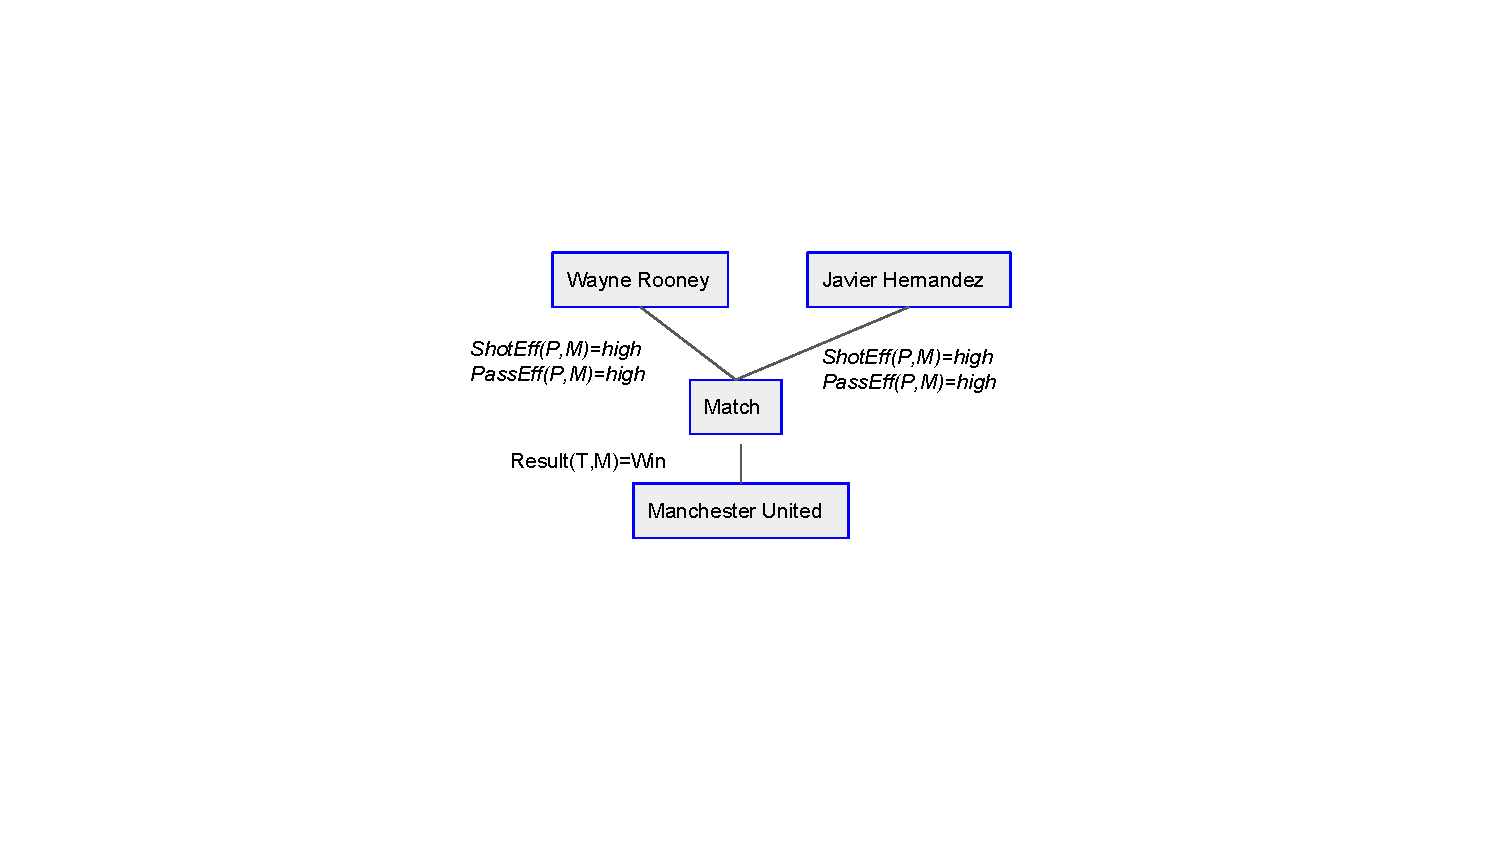
\includegraphics[width=0.7\textwidth] 
 	 				 	 						{figures/instancesofNetwork.pdf}
 	 				 	 						\caption{In the network representation, We have shown two instances of the conjunction: $\it{passEff(T,M)=hi}$, $\it{shotEff(T,M)=hi},$ $\it{Result(T,M)=win}$. We use the conjunctions to define subgraphs.  
 	 				 	 							%We show only the Markov blanket of the Results node to simplify. 
 	 				 	 							\label{fig:graphical_represetnaion}
 	 				 	 						}
 	 				 	 					\end{figure}
 	 				
 	 				%\begin{table} 
 	 				%	\captionsetup{singlelinecheck=off}
 	 				%			\caption[.]{\label{table:counts}Example of Grounding Count and Frequency for the conjunction \begin{displaymath} \it{passEff(T,M)=hi}, shotEff(T,M)=high, Result(T,M)=1.\end{displaymath} Counts are based on the 2011-2012 Premier League Season. We count only groundings $(\it{team},\it{match})$ such that $\it{team}$ plays in $\it{match}$. Each team, including Wigan Athletics, appears in 38 matches. The total number of team-match pairs is $38 \times 20 = 760$.
 	 				%			\label{MetricComputation}}
 	 				%			\centering
 	 				%			\resizebox{1\textwidth}{!}{
 	 				%				\begin{tabular}{|c|c|c|}
 	 				%					\hline
 	 				%					Database&Count or $\#_{D}(\Features = \set{\nodevalue})$&Frequency or $P_{D}(\Features = \set{\nodevalue})$\\\hline
 	 				%					Population&76& $76/760=0.10$\\\hline
 	 				%					Wigan Athletics&7&$7/38=0.18$\\\hline
 	 				%		
 	 				%					%Synthetic&40&280\\ \hline
 	 				%				\end{tabular}}
 	 				%				
 	 				
 	 
% 	 \section{Other Data Models}\label{sec:other}
% 	  In this section, we review some of the data models that have been previously used to represent the data for outlier detection task.
% 	  \begin{enumerate}
% 	  	
% 	  	\subsection{Attribute Vector Data Model}
% 	  		\textit{a) Attribute Vector Data Model:}
% 	  	
% 	  	By far most work on outlier detection considers atomic objects with flat feature vectors.
% 	  	, or nonhierarchical structures like time series. 
% 	  	This leads to an impedance mismatch: 
% 	  	The required input format for these outlier detection methods is a single data matrix, not a structured dataset. For example, one cannot provide a relational database as input. This mismatch is not simply a question of choosing a file format, but instead reflects a different underlying data model: complex objects with both attributes and component objects vs. atomic objects with attributes only. 
% 	  	
% 	  	It is possible to ``flatten'' structured data by converting it to unstructured feature vectors, for instance by using aggregate functions. 
% 	  	Flattening incurs some loss of information but allows us to apply the many feature vector methods.
% 	  	\cite{Elke2013}. 
% 	  		We evaluated the aggregation approach in this paper by applying three standard methods for outlier detection.
% 	  	for three major approaches to outlier detection: distance-based, density-based, and subspace clustering. 
% 	  	
% 	  	Subspace clustering methods (e.g., \cite{Muller2012,Kriegel2009}) are similar to our work in the sense that they aim to decompose a complex data space. They find complex deviations that are noticeable only in a data subspace. A common approach is to discover datapoints that show unexpected deviations in similar subspaces. Our approach instead develops a joint measure of how dissimilar the target object profile distribution is to the class distribution over the entire data space. Given that object and class distributions are represented by an object-oriented Bayesian network \cite{Koller1997}, the network structure defines subspaces. The joint divergence measure {\em mathematically decomposes} into subspace measures that quantify how dissimilar the target object profile distribution is in the subspaces defined by the network, compared to the class distribution in the same subspace.
% 	  	
% 	  	Work on atomic contextual  outliers \cite{Tang2013} is like ours in that it considers the distinctness of a target individual from a reference class. A reference class is not specified for each object,
% 	  	as a property of the object, 
% 	  	but is constructed as part of outlier detection. 
% 	  	Our work could be combined with a class discovery approach by providing a score of how informative the inferred classes are. 
% 	  	 	\begin{figure}
% 	  	 		\centering
% 	  	 		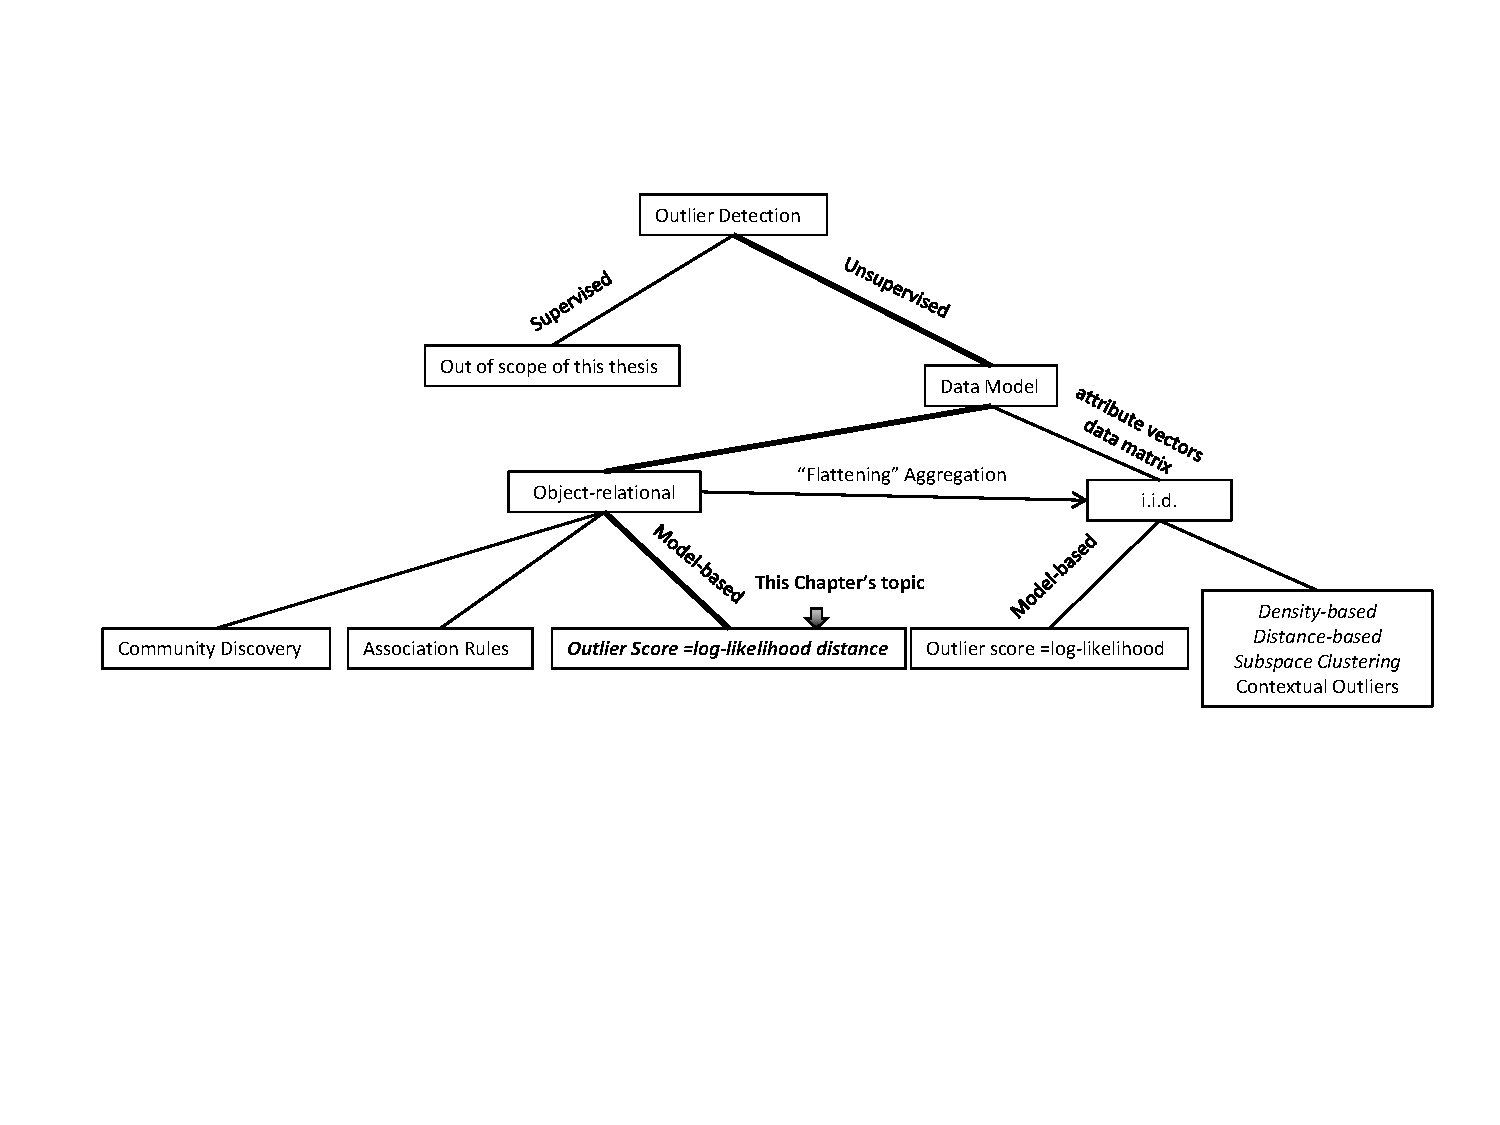
\includegraphics[width=1\textwidth] {figures/novelty-sep.pdf}
% 	  	 		\caption{A tree structure for related work on outlier detection for structured data. A path specifies an outlier detection problem, the leaves list major approaches to the problem. Approaches in italics appear in experiments.
% 	  	 			\label{fig:novelty}}
% 	  	 	\end{figure}
% 	  	\vspace{-5mm}
% 	  	
% 	  	We discuss related techniques in three types of structured data models: SQL (relational), XML (hierarchical), and OLAP (multi-dimensional). 
% 	  	
% 	  	For relational data, many outlier detection approaches aim to discover rules that represent the presence of anomalous associations for an individual or the absence of normal associations \cite{Maervoet2012,Gao2010}. The survey by \cite{Novak2009} unifies within a general rule search framework related tasks such as exception mining, which looks for associations that characterize unusual cases, subgroup mining, which looks for associations  characterizing important subgroups, and contrast space mining, which looks for differences between classes. Another rule-based approach uses Inductive Logic Programming techniques \cite{Angiulli2007}.
% 	  	,Angiulli2009}.
% 	  	While local rules are informative, they are not based on a global statistical model and do not provide a single outlier score for each individual. 
% 	  	
% 	  	A latent variable approach in information networks ranks potential outliers in reference to the latent communities inferred by network analysis \cite{Gao2010}. Our model aggregates information from entities and links of different types, but does not assume that different communities have been identified. 
% 	  	\subsection{Structured Data Models}	%\textit{b) }
% 	  	Koh {\em et al.}~\cite{koh2008} propose a method for hierarchical structures represented in XML document trees. Their aim is to identify feature outliers, not class outliers as in our work. Also, they use aggregate functions to convert the object hierarchy into feature vectors. Their outlier score is based on local correlations, and they do not construct a model.
% 	  	
% 	  	
% 	  	The multi-dimensional data model defines numeric measures for a set of dimensions. 
% 	  	A seminal approach to exploring a multi-dimensional datacube was presented by Sarawagi {\em et al.}~\cite{Sarawagi1998}. 
% 	  	The object and the multi-dimensional data models are similar in the respect that both objects and dimensions are ordered in a hierarchy. However, 
% 	  	The differences in the two data models mean that multi-dimensional outlier detection models~\cite{Sarawagi1998} do not carry over to object-relational outlier detection. (1) The object data model allows but does not require any numeric measures. In our datasets, all features are discrete. Nor do we assume that it is possible to aggregate numeric measures to summarize lower-level data at higher levels.  
% 	  	(2) In scoring a potential outlier object, our method considers other objects {\em both} below and above the target object in the component hierarchy. OLAP exploration methods consider only cells below or at the same level as the target cell. For example, in scoring a player, our method would consider features of the player's team.  
% 	  	Also, our proposed outlier score of an object is not determined by the outlier scores of its components, in contrast to the approach of Sarawagi {\em et al.}~\cite{Sarawagi1998}.
% 	  	 They use values such as the most unusual cell that is below a target cell.
% 	  	(3) Our approach models a joint distribution over features, exploiting correlations among features. Most of the OLAP-based methods consider only a single numeric measure at a time, not a joint model. \\ 
\section{Synthetic Datasets} \label{sec:synthetic}
 
 We generated three synthetic datasets with normal and outlier players using the distributions represented in the three Bayesian networks of Figure~\ref{fig:synthetic-bns}. 
 %The features $F_{1}$ and $F_{2}$ represent two features of players. 
 Each player participates in 38 matches, similar to the real-world data. The main goal of designing synthetic experiments is to test the methods on  easy to detect outliers. Each match assigns a value to each feature $F_i, i =  1,2$ for each player. 
 \begin{description}
 	\item\textbf{High Correlation}  Normal individuals exhibit a strong association between their features, outliers no association. Both normals and outliers have a close to uniform distribution over single features. See Figure~\ref{fig:synthetic-bns}(a).
 	\item\textbf{Low Correlation}  Normal individuals exhibit no association between their features, outliers have a strong association. Both normals and outliers have a close to uniform distribution over single features. See Figure~\ref{fig:synthetic-bns}(b).
 	\item\textbf{Single features}  Both normal and outlier individuals exhibit a strong association between their features. In normals, 90\% of the time, feature 1 has value 0. For outliers, feature 1 has value 0 only 10\% of the time. See Figure~\ref{fig:synthetic-bns}(c).
 \end{description}
 We used the $\it{mlbench}$ package in $\it{R}$ to generate synthetic features in matche and followed these distributions for 240 normal players and 40 outliers. We followed the real-world Opta data in terms of number of normal and outlier individuals. %The scores are used to rank all 280 players. 
 
 \begin{figure*}[htbp]
 	\centering
 	\resizebox{1\textwidth}{!}{
 		\includegraphics%[width=0.3\textwidth] 
 		{figures/figure1kddCropped.pdf}
 	}
 	\caption{Illustrative Bayesian networks. The networks are not learned from data, but hand-constructed to be plausible for the soccer domain. (a) High Correlation;
 		% The outlier distribution misses a correlation that is present in the normal population. The single feature distributions are uniform in both distributions. 
 		(b) Low Correlation;
 		% The outlier object exhibits a correlation that is not present in the normal population. The single attribute distributions are uniform in both distributions.
 		(c) Single Attributes.
 		%Correlations are the same, but the single feature distributions are not.
 		\label{fig:synthetic-bns}}
 \end{figure*}
 
 
 \section{Real-world Datasets} \label{sec:real-world-data}
 In this dissertation, real world data tables are prepared from Opta data~\cite{opta-original} and IMDb~\cite{IMDb-original}.% Our datasets and code are available on-line~\cite{bib:url}.
 Table~\ref{table:Features-chapter3} lists the populations and features. Table~\ref{table:StatsChapter3} shows summary statistics for the datasets. 
 %	
 %	\begin{table}[htbp]
 %		\centering
 %		\resizebox{0.4\textwidth}{!}{
 %			\begin{tabular}{|c|p{5cm}|}
 %				\hline
 %				Individuals & Features\\ \hline
 %				\begin{tabular}{c}Soccer-Player\\per Match \end{tabular} & $\it{TimePlayed}$,$\it{Goals}$,$\it{SavesMade}$,
 %				$\it{ShotEff}$,$\it{PassEff}$,$\it{WinningGoal}$,
 %				$\it{FirstGoal}$,$\it{PositionID}$, $\it{TackleEff}$,$\it{DribbleEff}$,
 %				$\it{ShotsOnTarget}$ \\ \hline
 %				\begin{tabular}{c}Soccer-Team\\per Match \end{tabular} & $\it{Result}$,$\it{TeamFormation}$,$\sum\it{Goals}$,
 %				$\mu\it{ShotEff}$,$\mu\it{PassEff}$,$\mu\it{TackleEff}$, 
 %				$\mu\it{DribbleEff}$. \\ \hline
 %				IMDB-Actor & $\it{Quality}$, $\it{Gender}$ \\ \hline
 %				IMDB-Director & $\it{Quality}$,$\it{avgRevenue}$\\ \hline
 %				IMDB-Movie&$\it{year}$,$\it{isEnglish}$,$\it{Genre}$,$\it{Country}$, $\it{RunningTime}$, $\it{Rating}$ by User\\ \hline
 %				IMDB-User& %$\it{Rating}$,
 %				$\it{Gender}$, $\it{Occupation}$.\\ \hline
 %			\end{tabular}}	
 %			\caption{Attribute Features. $\mu$ = average, $\\sum$ = sum. For relationships please see text.\label{table:Features}}
 %			
 %		\end{table}
 
 
 \begin{table}[htbp]
 	\centering
 	\resizebox{0.6\textwidth}{!}{
 		\begin{tabular}{|c|p{5cm}|}
 			\hline
 			Individuals & Features\\ \hline
 			\begin{tabular}{c}Soccer-Player\\per Match \end{tabular} & $\it{TimePlayed}$,$\it{Goals}$,$\it{SavesMade}$,
 			$\it{ShotEff}$,$\it{PassEff}$,$\it{WinningGoal}$,
 			$\it{FirstGoal}$,$\it{PositionID}$, $\it{TackleEff}$,$\it{DribbleEff}$,
 			$\it{ShotsOnTarget}$ \\ \hline
 			\begin{tabular}{c}Soccer-Team\\per Match \end{tabular} & $\it{Result}$,$\it{TeamFormation}$,
 			$\sum\it{Goals}$,$\mu\it{ShotEff}$,$\mu\it{PassEff}$,
 			$\mu\it{TackleEff}$,$\mu\it{DribbleEff}$. \\ \hline
 			IMDB-Actor & $\it{Quality}$, $\it{Gender}$ \\ \hline
 			IMDB-Director & $\it{Quality}$,$\it{avgRevenue}$\\ \hline
 			IMDB-Movie&$\it{year}$,$\it{isEnglish}$,$\it{Genre}$,$\it{Country}$, $\it{RunningTime}$, $\it{Rating}$ by User\\ \hline
 			IMDB-User& %$\it{Rating}$,
 			$\it{Gender}$, $\it{Occupation}$.\\ \hline
 		\end{tabular}}
 		\caption{Attribute features.% $\mu$ = average, $\\sum$ = sum. For relationships please see text.
 			\label{table:Features-chapter3}}
 		
 	\end{table}
 	\paragraph{Soccer Data} 
 	The Opta data were released by Manchester City. 
 	It lists all the ball actions within each game, by each player, for the 2011-2012 season. 
 	%The data consists of information about the actions of a single player in a given match 
 	%from 2011 to 2012. 
 	Number of goals, passes, fouls, tackles, saves and blocks, and also the position 
 	assigned to a player in a match, are examples of the information associated with each player.
 	%Information about the teams in a season, such as number of home wins, draws or away wins can be extracted by massaging the data. 
 	%[The information can be visualized as a heterogeneous network that links players to teams, and teams to matches. ]
 	For each player in a match, our dataset contains eleven player features.
 	% like $\it{TimePlayed}(\P,\M)$.
 	For each team in a match, there are five features computed as player feature aggregates, as well as the team formation and the result (win, tie, loss). 
 	There are two relationships, $\it{Appears\_Player}(\P,\M)$, $\it{Appears\_Team}(\T,\M)$. 
 	%We store the data in a relational database, with a table for each base population and a table for each relationship.
 	We refer to the Premier League data as the {\em Soccer} dataset.
 	Table~\ref{table:StatsChapter3} shows summary statistics for the datasets. 
 	\begin{table}
 		\centering
 		\resizebox{0.8\textwidth}{!}{
 			\begin{tabular}{|l|l|l|l|} \hline
 				\multicolumn{2}{|c|}{Premier League Statistics}& \multicolumn{2}{|c|}{IMDB Statistics}\\
 				\hline
 				Number Teams&20&Number Movies&3060 \\ \hline
 				Number Players&484&Number Directors&220 \\ \hline
 				Number Matches&380&Number Actors&98690  \\ \hline
 				avg player per match&26.01& avg actor per movie&36.42  \\ \hline
 			\end{tabular} 
 		}
 		\caption{Summary statistics for the IMDb and the Premier League datasets}
 		\label{table:StatsChapter3}
 	\end{table}
 	
 	\paragraph{IMDB Data} 
 	The Internet Movie Database (IMDB) is an on-line database of information related to films, television programs and video games.
 	The IMDB website offers a dataset containing information on cast, crew, titles, technical details and biographies in a set of compressed text files. 
 	We preprocessed the data like, \cite{Peralta2007}, to obtain a database with seven tables, one for each population and one for the three relationships: $\it{Rated}(\user,\movie)$, $\it{Directs}(\director,\movie)$, and $\it{ActsIn}(\actor,\movie)$.
 	
 	%	Table~\ref{table:Features-prime} lists relationships and the number of features. 
 	%					\begin{table}[htbp]
 	%								\caption{Relationships and Example Features in Real-World Datasets.
 	%									%For relationships please see text.
 	%									\label{table:Features}}
 	%						\centering
 	%						\resizebox{0.6 \textwidth}{!}{
 	%							\begin{tabular}{|l|c|l|}
 	%								\hline
 	%								Path/Object Type & \#Attributes&Example\\ \hline
 	%								\begin{tabular}{c}Player-Team-Match \end{tabular} & 11&ShotEff \\ \hline
 	%								\begin{tabular}{c}Team-Match \end{tabular} & 7&TeamFormation \\ \hline\hline
 	%								Actor & 2&Quality \\ \hline
 	%								Director & 2&AvgRevenue\\ \hline
 	%								Movie&5&Genre\\ \hline
 	%								User& 2&Occupation\\ \hline
 	%								User-Movie & 1&Rating \\\hline
 	%								Actor-Movie & 1&Cast\_Position\\\hline
 	%							\end{tabular}}
 	%					
 	%						\end{table}
 	%\footnote{Commented table of relationships and features}
 	%					\begin{LaTeXdescription}
 	%						\item[Soccer Data]
 	%						The Opta data were released by Manchester City. 
 	%						It lists all the ball actions within each game by each player, for the 2011-2012 season.
 	%						\item[IMDb Data]
 	%						The Internet Movie Database (IMDb) is an online database of information related to films, television programs, and video games.
 	%						The IMDb website offers a dataset containing information on cast, crew, titles, technical details and biographies in a set of compressed text files \cite{Peralta2007}.
 	%					\end{LaTeXdescription}
 	
 	%\subsection{Outlier and Contrast Classes.}
 	
 	In real-world data there is no ground truth about which objects are outliers. To address this issue we employ a one-class design: we learn a model for the class distribution, with data from only that class. We then rank all individuals from the normal class, together with all objects from a contrast class treated as outliers, in order to test whether an outlier score recognizes objects from the contrast class as outliers.
 	%		distinguishes objects from the normal class from objects in the contrast class. 
 	Table~\ref{MetricComputation} shows the normal and contrast classes for three different datasets.  In-class outliers are possible, e.g. unusual strikers are still members of the striker class. Chapter~\ref{chap:five} describes a few in-class outliers. In the soccer data we considered only individuals who played more than 5 matches out of a maximum 38. 
 	
 	\begin{table}
 		\caption{Outlier/normal objects in real-world datasets. }
 		\label{MetricComputation}
 		\centering
 		\resizebox{0.5\textwidth}{!}{
 			\begin{tabular}{|c|c|c|c|}
 				\hline
 				Normal&\#Normal&Outlier&\#Outlier\\\hline
 				Striker & 153 & Goalie&22\\ \hline
 				Midfielder & 155 & Striker&74\\ \hline
 				Drama & 197 & Comedy&47\\ \hline
 				%Synthetic&40&280\\ \hline
 			\end{tabular}}
 			
 		\end{table}
 		
 	\section{Statistical Models} \label{sec:otherStat}
 	
 	We use notation and terminology from previous work \cite{Poole2003,Chiang2012,Lippi2011,Domingos2009}. While we do not introduce any new terminology, we combine concepts from different areas, such as propositionalization and log-linear models. 
 	
 	%				\subsection{Predicate Language}
 	%				
 	%				We employ the notation of Chiang and Poole \cite{Chiang2012} for logical syntax, as follows.
 	%				%
 	%				Constants are expressed in lower-case, e.g. $\it{joe}$, and are used to represent individuals. A type is associated with each individual, e.g. $\it{joe}$ is a person. We use $D(\tau)$ to represent a domain of type $\tau$, which is the set of individuals of type $\tau$. A {\em logical variable} is written in upper case. A logical variable is also typed, e.g. $\it{Person}$ denotes some member of $D(\tau)$. A relation is given by 
 	%				$$r : \Omega \rightarrow V_{r}$$
 	%				where $r$ is the name of the relation, $\Omega_{r}=D(\tau_{1})\times \ldots \times D(\tau_{a})$ is the domain of the relation, and $T_{r}=(\tau_{1},\ldots,\tau_{a})$ is the type of the relation. $V_{r}={v_{1},\ldots,v_{k}}$ is the range of the relation. Number $a$ and $k$ are positive integers denoting the {\em arity} and {\em size} of $r$. An {\em atom} is an expression of the form $r(\sigma_{1},\ldots,\sigma_{a})$ where each $\sigma_{i}$ is either a constant or logical variable. If all of $\sigma_{1},\ldots,\sigma_{a}$ are constants, $r(\sigma_{1},\ldots,\sigma_{a})$ is a {\em ground atom}.
 	%				
 	%				A {\em literal} specifies the value of an atom e.g. $r(X_{1},\ldots,X_{a})=v$ where $v \in V_{r}$. A literal is also a {\em formula}. Formulae with multiple literals are formed using connectives $\wedge$ and or $\vee$. Connecting literals using only $\wedge$ forms a {\em conjunctive formula } or {\em conjunction}. A formula that contains no logical variables is a {\em ground} formula.
 	%				%, is a proposition.
 	%				%A {\em disjunctive formula} or {\em disjunction} is formed using only $\vee$. \\
 	%				
 	%				A substitution is a set $\{X_{1} \textbackslash x_{1}, \ldots, X_{k}\textbackslash x_{k}\}$ where $X_{i}$ are distinct logical variables and $x_{i}$ are constants. When applied to a formula $f$, each occurrence of $X_{i}$ in $f$ is replaced with $x_{i}$. We denote the application of a substitution 
 	%				%$\{X_{1} \textbackslash x_{1}, \ldots, X_{k}\textbackslash x_{k}\}$ 
 	%				to $f$ as $f\{X_{1} \textbackslash x_{1}, \ldots, X_{k}\textbackslash x_{k}\}$. 
 	%				Consider a formula $f$ containing logical variables $X_{1}, \ldots,X_{n}$, where each $X_{i}$ has type $\tau_{i}$. The {\em grounding space} of $f$, is the set of all possible grounding substitutions for $f$, given by 
 	%				$$\{\{X_{1}\textbackslash x_{1}, \ldots, X_{n}\textbackslash x_{n}\}:x_{i} \in D(\tau_{i}) \mbox{ for } i=1,\ldots,n\}.$$
 	%				
 	%				%	Given some formula $f$ containing logical variables $X_{1}, \ldots,X_{n}$, where each $X_{i}$ has type $\tau_{i}$, let the domain of $f$ be $\Omega_{f}=D(\tau_{i}\times \tau_{n})$. The {\em substitution space} of $f$, $\Gamma_{f}$, is the set of all possible grounding substitutions for $f$, given by 
 	%				%	$$\Gamma_{f}=\{\{X_{1}\textbackslash x_{1}, \ldots, X_{n}\textbackslash x_{n}\}:(x_{1},\ldots,x_{n})\in \Omega_{f}\}.$$
 	%				
 	%				A \emph{database} $\D$ specifies for each ground literal whether the literal is true in the database or not. A ground conjunction is true in a database if all of its conjuncts are true. The \emph{count} of groundings satisfying formula $\formula$ with respect to a database $\D$ is denoted as $\grounds_{\D}(\formula)$.
 	%	
 	
 	\subsection{Bayesian Network}
 	We adopt  
 	the Parametrized Bayes net (PBN) formalism \cite{Poole2003} that combines Bayes nets with logical syntax for expressing relational concepts. 
 	
 	
 %	\subsubsection{Bayesian Networks}
 	
 	A {\bf Bayesian Network (BN) structure} $\model$ is a directed acyclic graph (DAG)  whose nodes comprise a set of random variables \cite{Pearl1988}. Depending on the context, we interchangeably refer to the nodes  and variables of a BN. Fix a set of variables $\Features = \{\feature_{1},\ldots,\feature_{n}\}$. 
 	%These are attributes of objects, which can and typically do belong to different classes. In statistical terms, each attribute defines a random variable. 
 	The possible values of $\feature_{i}$ are enumerated as $\{\nodevalue_{i1},\ldots,\nodevalue_{i\states_{i}}\}$. The notation $P(\feature_{i} = \nodevalue)\equiv P(\nodevalue)$ denotes the probability of variable $\feature_{i}$ taking on value $\nodevalue$. We also use the vector notation $P(\Features = \set{\nodevalue}) \equiv P(\set{\nodevalue})$ to denote the joint probability that each variable $\feature_{i}$ takes on value $\set{\nodevalue}_{i}$. 
 	
 	
 	The conditional probability parameters of a Bayesian network specify the distribution of a child node given an assignment of values to its parent node. For an assignment of values to its nodes, a BN defines the joint probability as the product of the conditional probability of the child node value given its parent values, for each child node in the network. This means that the log-joint probability can be {\em decomposed} as the node-wise sum
 	
 	\begin{equation} \label{eq:bn}
 	\ln P(\Features = \set{\nodevalue};\model,\parameters) = \sum_{i=1}^{n} \ln \parameter(\set{\nodevalue}_{i}|\set{\nodevalue}_{\parents_{i}})
 	\end{equation}
 	
 	where $\set{\nodevalue}_{i}$ resp. $\set{\nodevalue}_{\parents_{i}}$ is the assignment of values to node $\feature_{i}$ resp. the parents of $\feature_{i}$ determined by the assignment $\set{\nodevalue}$. 
 	%The function $\ln$ is the binary logarithm base 2. 
 	To avoid difficulties with $\ln(0)$, here and below we assume that joint distributions are positive everywhere. Since the parameter values $\parameters$ for a Bayes net define a joint distribution over its nodes, they therefore entail a marginal, or unconditional, probability for a single node. We denote the \textbf{marginal probability} that node $\feature$ has value $\nodevalue$ as $P(\feature = \nodevalue;\model,\parameters) \equiv \parameter(\nodevalue)$. In the following chapters, we use the term Bayesian network model to refer to a network structure with parameters (i.e., a pair $(\model,\parameters)$); for brevity, we also use the terms ``Bayesian network'' or ``model''. 
 					A \textbf{Parametrized Bayesian Network Structure} (PBN) is a Bayesian network structure  whose nodes are PRVs~\cite{Poole2003}.  				The relationships and features in an object database define a set of nodes for Bayes net learning; see Figure~\ref{fig:bns-chap3}.
 	\paragraph{Example.} Figure~\ref{fig:bns-chap3} shows an example of a Bayesian network model and associated joint and marginal probabilities.
 	%
 	%\footnote{\textbf{Sarah}: add marginal probability P(res=win) for object parameters}
 	\begin{figure}[t]
 		\centering
 		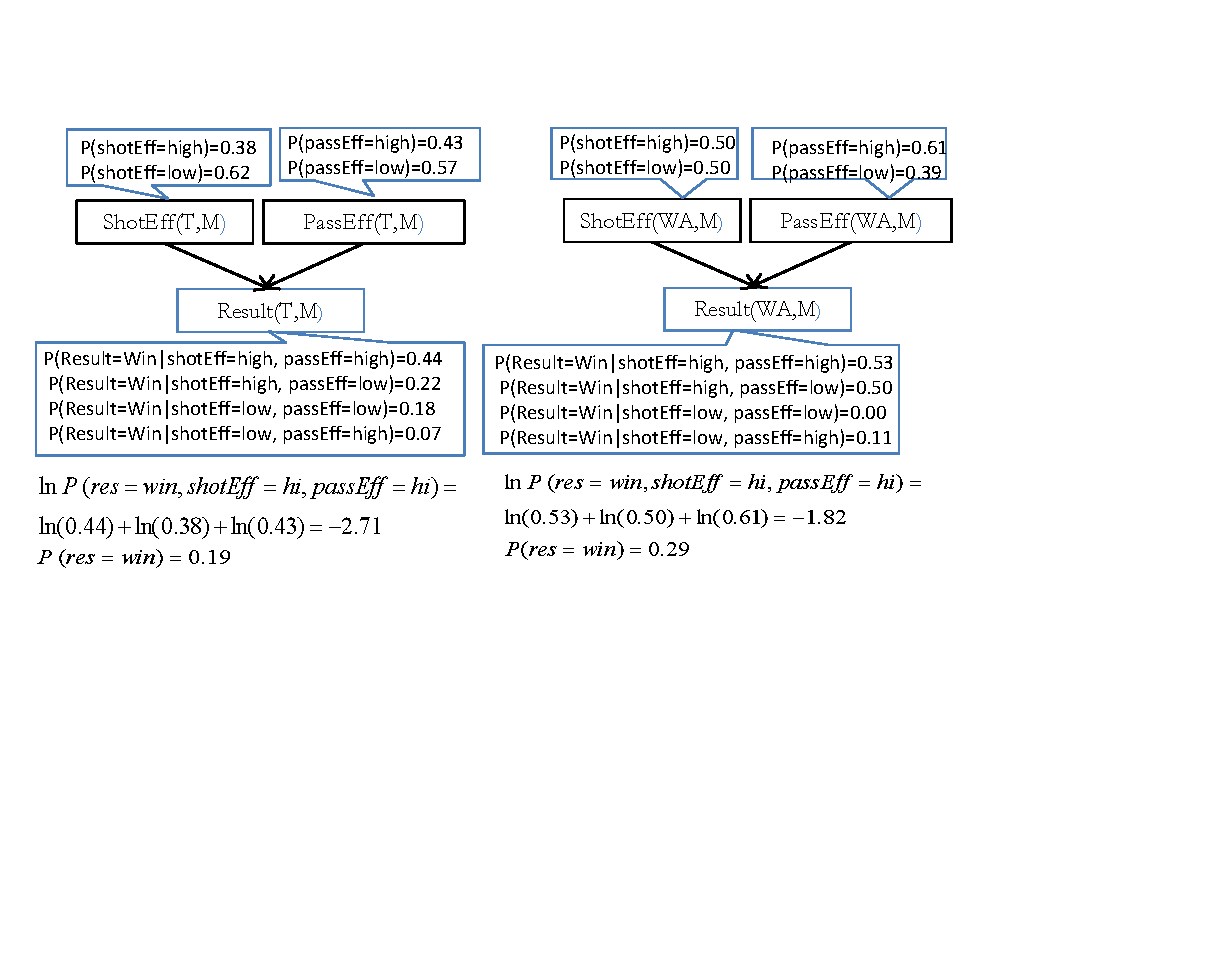
\includegraphics[width=1\textwidth] 
 		{figures/bnuncropped}
 		\caption{Example of joint and marginal probabilities computed from a toy Bayesian network structure. The parameters were estimated from the  Premier League dataset. (Top): A class model Bayesian network $\model_{\class}$ for all teams with class parameters $\parameters_{\class}$. (Bottom): The same Bayesian network structure with object parameters $\parameters_{\object}$ learned for Wigan Athletics ($T = WA$). Our model-based methods outlier scores compare the data likelihood of the class parameters and the object parameters.
 			%We show only the Markov blanket of the Results node to simplify. 
 			\label{fig:bns-chap3}
 		}
 	\end{figure}
 	
 
 	
 	%	\begin{figure}[t]
 	%		\centering
 	%		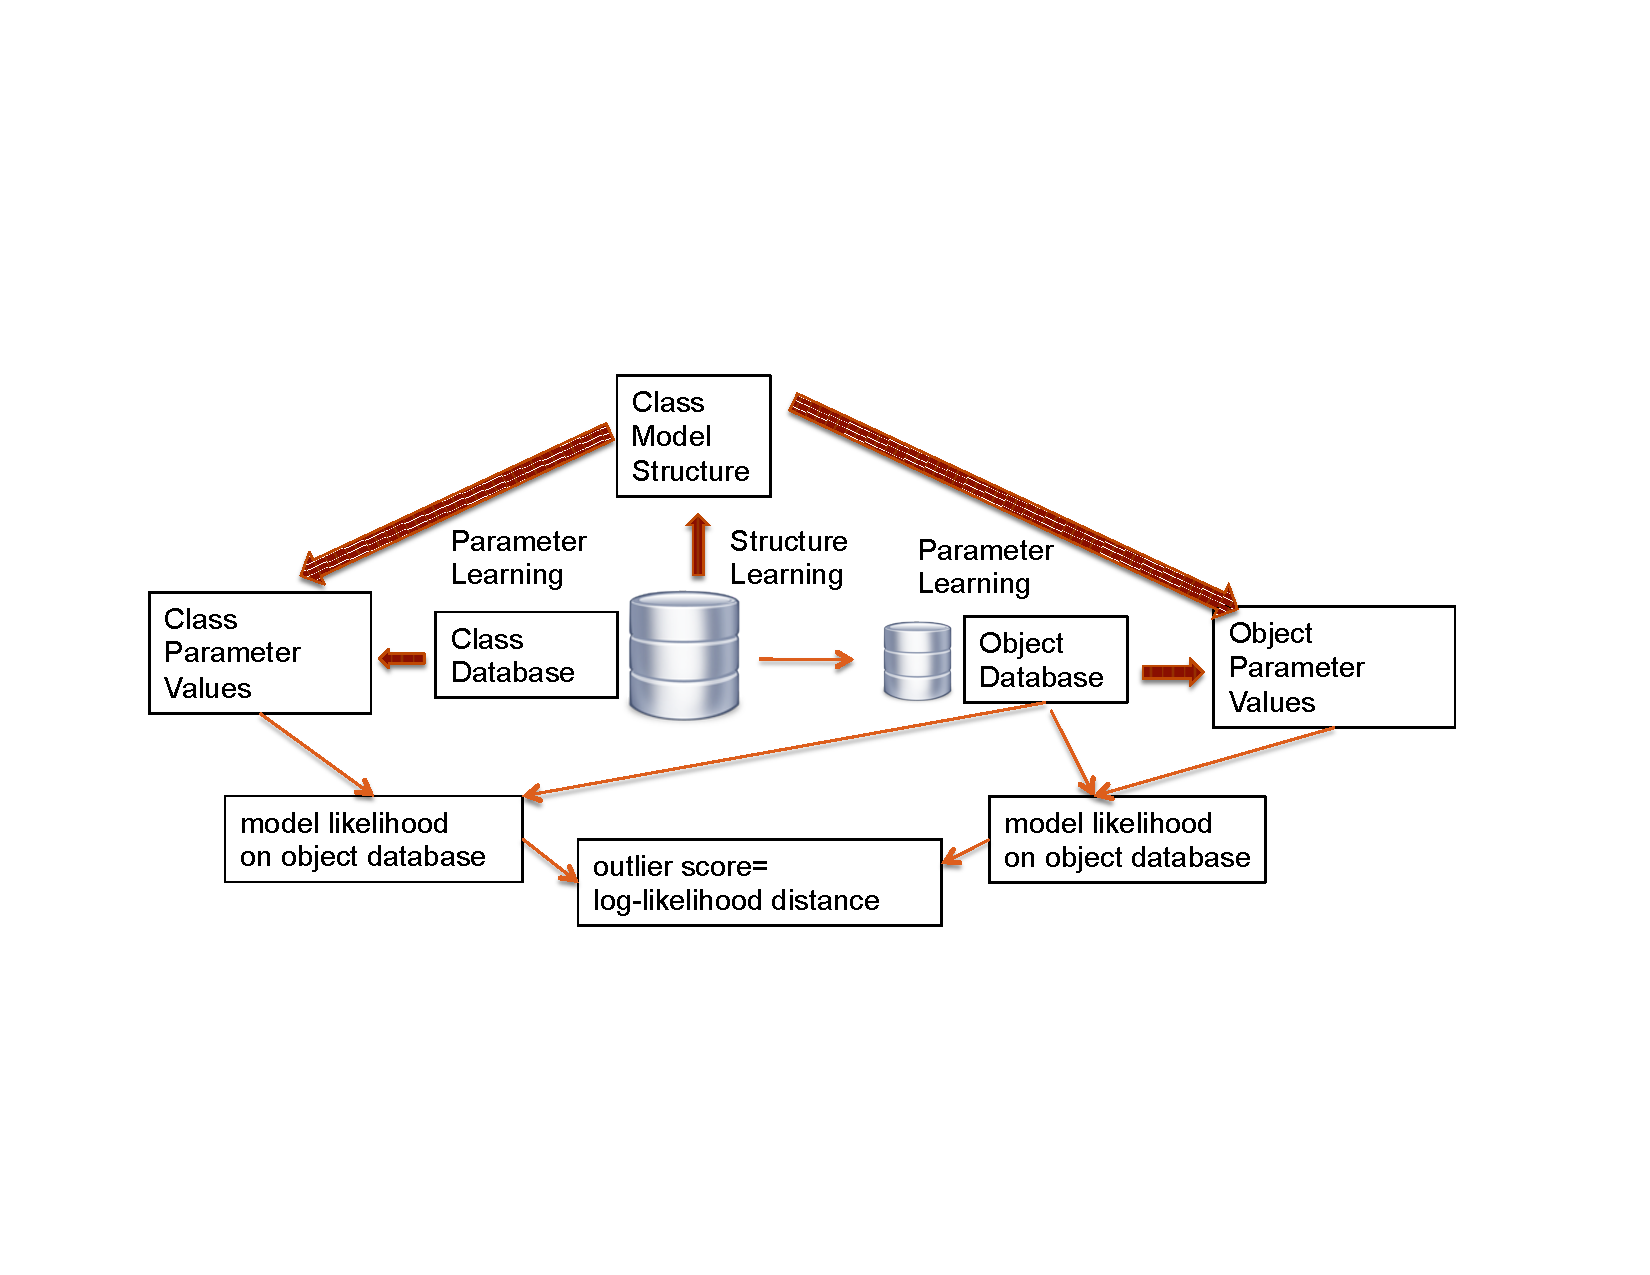
\includegraphics[width=1\textwidth]{figures/flow.pdf}
 	%		
 	%		\caption{Computation of outlier score. 
 	%			\label{fig:flow}}
 	%	\end{figure}
 	%				\begin{figure}
 	%				\centering
 	%				\resizebox{0.9\textwidth}{!}{
 	%				
 	%				\subfigure{
 	%				  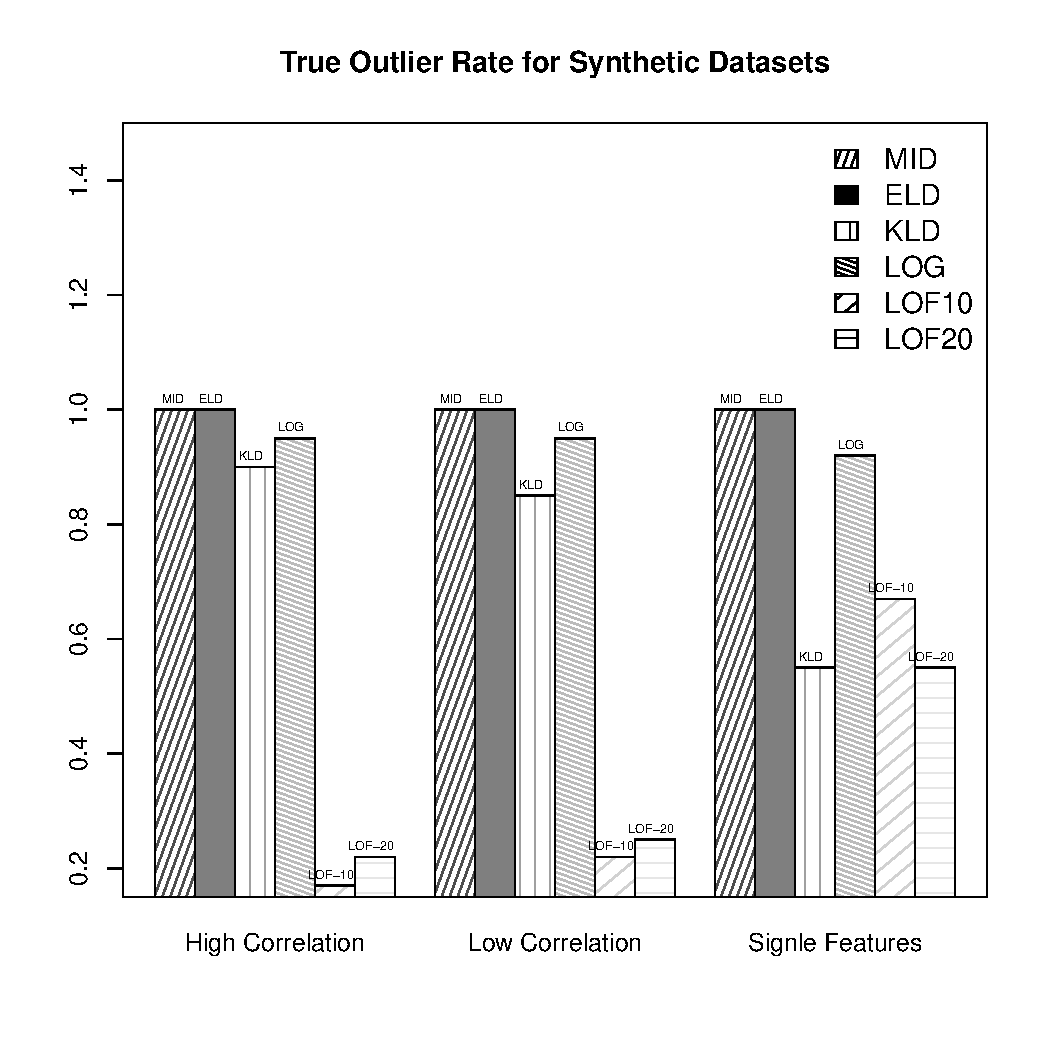
\includegraphics[height=70mm, width=70mm] {figures/TPR-Synthetic.pdf}
 	%				}
 	%				\subfigure{
 	%				  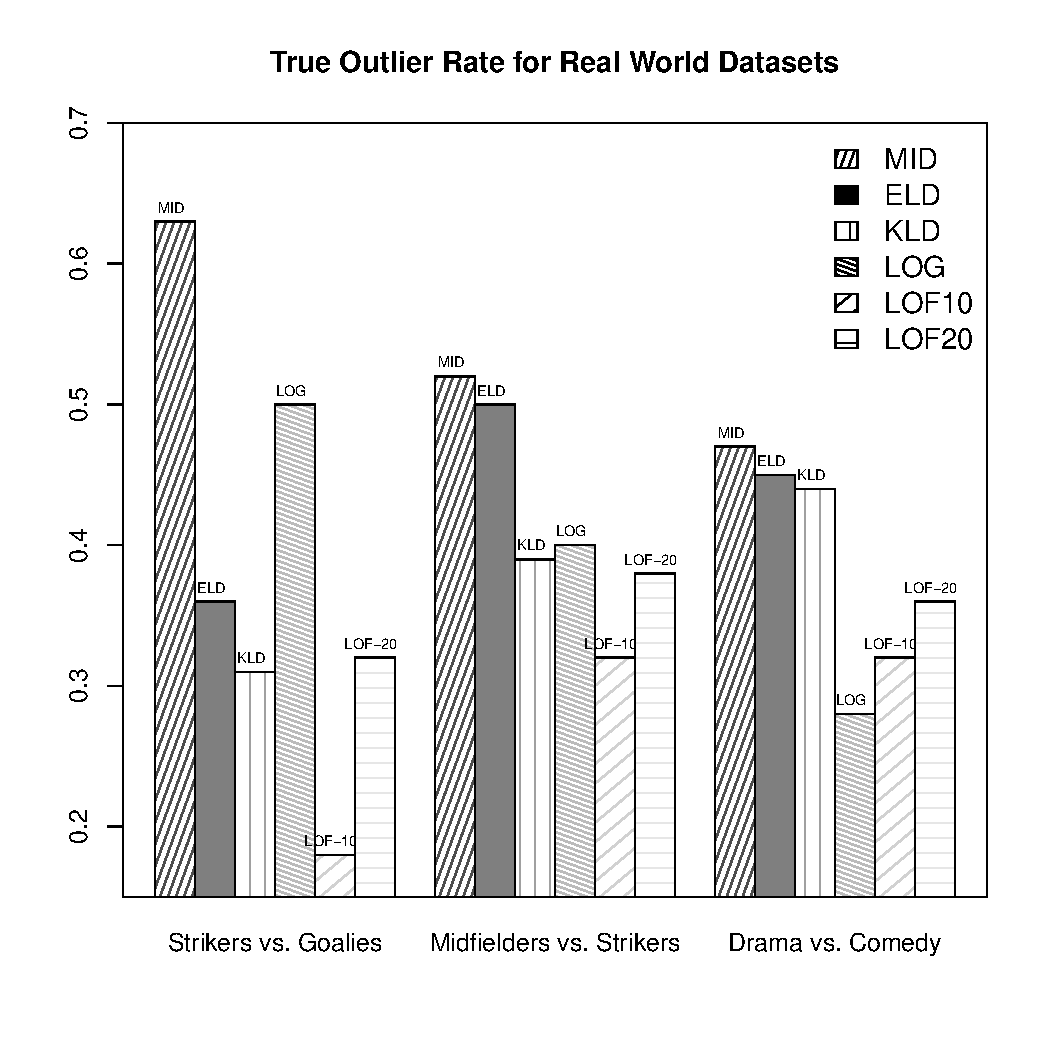
\includegraphics[height=70mm, width=70mm] {figures/TPR-All.pdf}
 	%				
 	%				 }
 	%				 }
 	%				
 	%				\caption{Comparison of Object Outlier Metrics}
 	%				\label{fig:synthetic}
 	%				\end{figure}
 	%				
 	
 	%				\begin{figure}
 	%					\centering
 	%					\begin{subfigure}{0.4\textwidth}
 	%						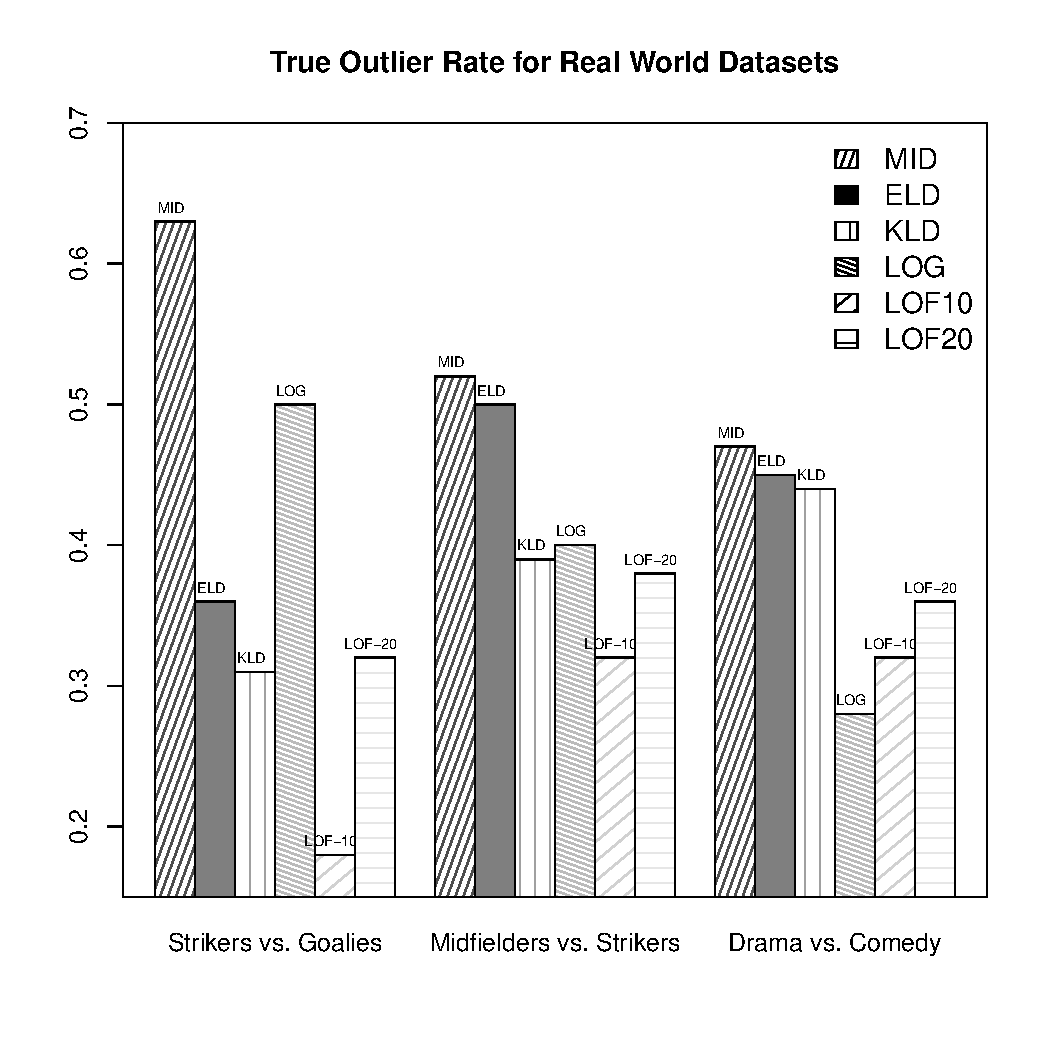
\includegraphics[width=1\linewidth]{figures/TPR-All.pdf}
 	%						\caption{}
 	%						\label{fig:Ng1} 
 	%					\end{subfigure}
 	%					
 	%					\begin{subfigure}{0.4\textwidth}
 	%						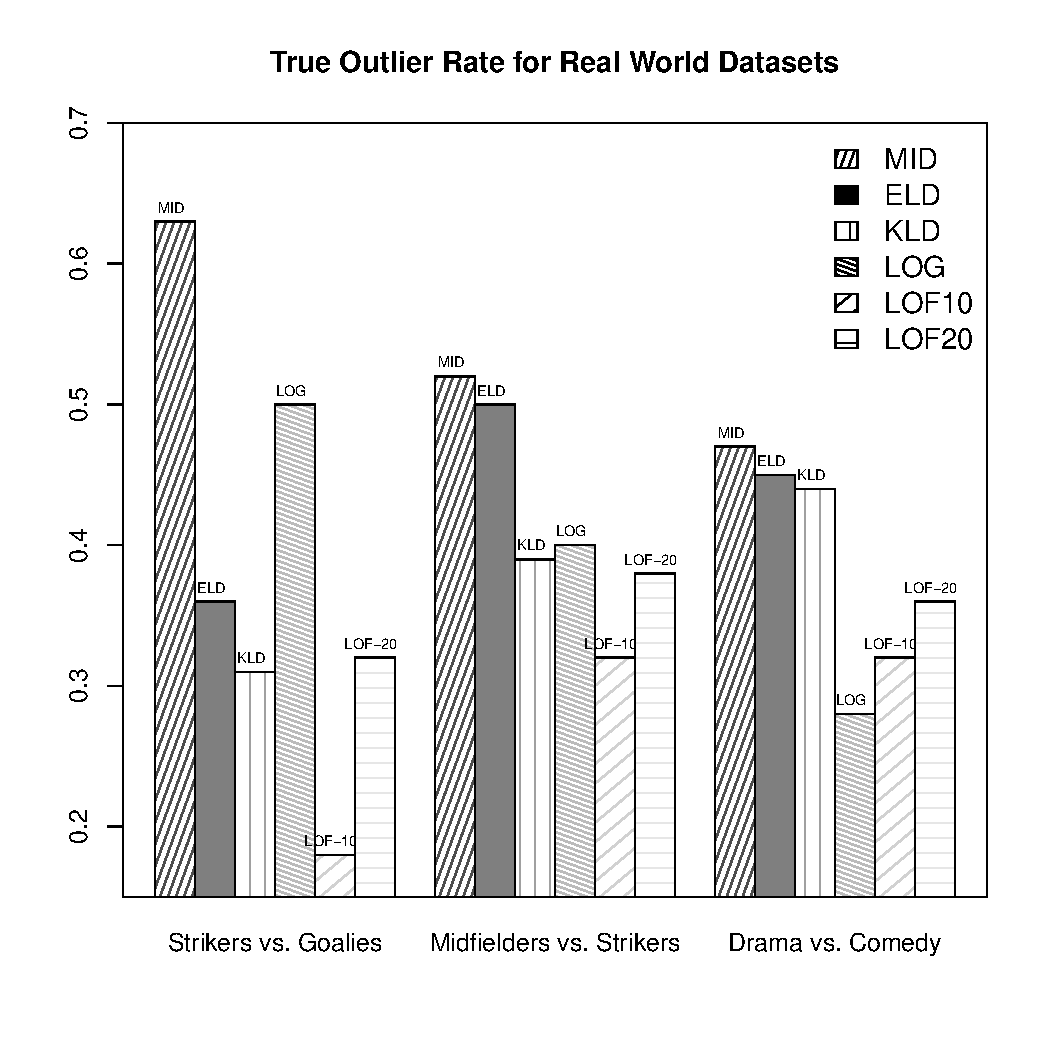
\includegraphics[width=1\linewidth]{figures/TPR-All.pdf}
 	%						\caption{}
 	%						\label{fig:Ng2}
 	%					\end{subfigure}
 	%					
 	%					\caption[Two numerical solutions]{(a) Numerical solutions for the small-time system 
 	%						with a constant-curvature body shape showing the scaled leading-order veritcal 
 	%						reaction force $N_0$ versus the scaled body mass $M$ for various values of $g$. 
 	%						Again, $I=M$ for definiteness and $A=0.7$. (b) As for (a) but over a wider range of 
 	%						values of $M,I$.}
 	%				\end{figure}
 	
  				%			\end{table}
 				
 				%[Example of counts, frequencies]
 				% For simplicity only, suppose that the only matches and players in the season are those shown in Table~\ref{table:data}. Then the attribute value $\it{First\_goals} = 0$ occurs with frequency $1/2$ in the object distribution $P_{\it{si}}$ for Silca. In the player class distribution $P_{\it{Player}}$, the attribute value $\it{First\_goals} = 0$ occurs with frequency $4/5$. So Silva is somewhat less likely to score no goal than a randomly selected player.
 			%	\subsubsection{Bayesian Networks for Relational Data}
 				
 
 				%For most of the paper we refer to PBNs simply as Bayesian networks, and to PRVs simply as random variables. 
 				%The learn-and-join algorithm is the state-of-the-art Bayes net learning method for relational data, based on model search in the lattice of relationship joins \cite{Schulte2012}. The LAJ algorithm takes as input a relational database and outputs a Parametrized Bayes net structure.
 				%We review the algorithm very briefly; for further details please see \cite{Schulte2012}. 
 				%The algorithm builds a Bayes net for an entire database by level-wise search through the {\em lattice of relationship chains.} This is the lattice of relationship sets that are connected by shared first-order variables.
 				%%; see Figure~\ref{fig:lattice}.  
 				%%We describe the fundamental ideas of the algorithm; for further details please see \cite{Schulte2012}. 
 				%The user chooses a single-table Bayes net learner. The learner is applied to base population data tables. Then the learner is applied to data tables for relationship chains of size $s,s+1,\ldots$, with the constraint that the models for larger join tables inherit the absence or presence of learned edges from smaller join tables. 
 				%

 				

 				% shows a sample PBN.
 				
 				
 				%We use the following notation.
 				
 				%\begin{figure}[ht]
 				%\centering
 				%   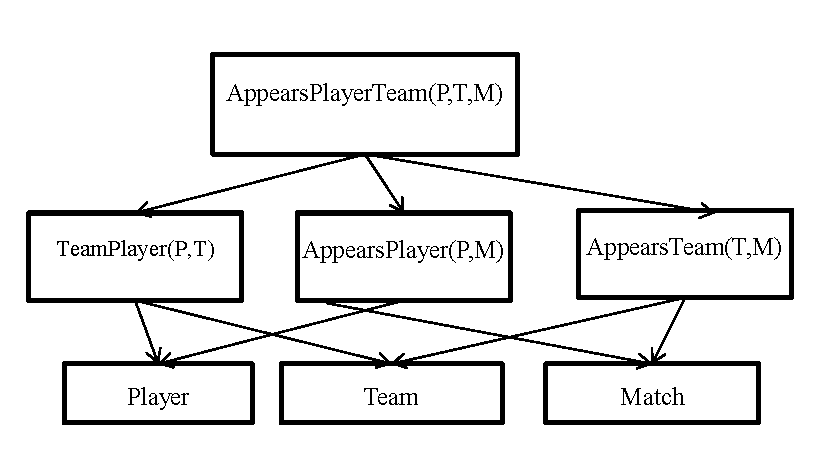
\includegraphics[width=0.3\textwidth] {lattice}
 				% \caption{Lattice of Premier League dataset.
 				% %We show only the Markov blanket of the Results node to simplify. 
 				% \label{fig:lattice}}
 				%\end{figure}
 				
 				
 				
 				
 				%\begin{itemize}
 				%\item $\D_{\population}$ is the database for the entire population; cf. Table~\ref{table:data}.
 				%\item $\D_{\target}$ is the restriction of the input database to the target object; cf. Table~\ref{table:object}. 
 				%\item $\M_{\population}$ is a model (e.g., Bayesian network) learned with $\D_{\population}$ as the input database; cf. Figure~\ref{fig:bns}(a).
 				%\item $\M_{\target}$ is an object model (e.g., Bayesian network) learned with $\D_{\target}$ as the input database; cf. Figure~\ref{fig:bns}(b).
 				%\end{itemize}
 							
 %	\subsection{Logical Concepts}
% 	We follow the description of propositionalization in Lippi {\em et al.} \cite{Lippi2011}, where the input to a propositionalizer is a relational database, and the output is a pseudo-\iid data view. 
% 	We adopt a term-based notation for logical concepts~\cite{Poole2003,Chiang2012}. Constants such as $\it{rooney}$, $123$ are used to represent individuals.
% 	% A \textbf{population} is a set of individuals. 
% %	A functor is a function or predicate symbol, denoting a function that is applied to individuals. Each functor has a set of possible values (constants) called the \textbf{domain} of the functor. The domain of a \textbf{predicate} is $\{\true,\false\}$. Predicates are usually written with uppercase Roman letters, other terms with lowercase letters.
% 	
% 	A predicate of arity at least two is a \textbf{relationship} functor. Relationship functors specify which objects are linked. Other functors represent \textbf{features} or \textbf{attributes} of an object or a tuple of objects (i.e., of a relationship).
% 	A \textbf{term} is of the form $f(\term_{1},\ldots,\term_{k})$ where $\functor$ is a functor %(either a function symbol or a predicate symbol) 
% 	and each $\term_{i}$ is a first-order variable or a constant. 
% 	An {\em atomic assignment} specifies the value of a term e.g. $\functor(\term_{1},\ldots,\term_{k})=v$ where $v$ is in the domain of functor $\functor$. 
% 	%A literal is also a {\em formula}. 
% 	%		Formulae with multiple literals are formed using connectives $\wedge$ and or $\vee$. 
% 	Connecting assignments using only $\wedge$ forms a {\em conjunctive formula } or {\em conjunction}. In this dissertation we use conjunctive formulas only. A term/literal/formula is \textbf{ground} if it contains no first-order variables; otherwise it is a first-order term/literal/formula. 
% 	
% 	An object-relational database $\D$ specifies the values of all ground terms, and hence whether a ground literal is true or not. A ground conjunction is true in a database if all of its conjuncts are true.
% 	% A \textbf{grounding} is a set $\{X_{1} \backslash x_{1}, \ldots, X_{k}\backslash x_{k}\}$ where $X_{i}$ are distinct logical variables and $x_{i}$ are constants. When applied to a formula, each occurrence of $X_{i}$ is replaced with $x_{i}$. 
% 	%We denote the application of a substitution 
% 	%$\{X_{1} \backslash x_{1}, \ldots, X_{k}\backslash x_{k}\}$ 
% 	%		to $f$ as $f\{X_{1} \backslash x_{1}, \ldots, X_{k}\backslash x_{k}\}$.
% 	%		
% 	The count of groundings that satisfy (make true) formula $\formula$ with respect to a database $\D$ is denoted as $\grounds_{\D}(\formula)$.	
 	
 	
 	\subsection{Markov Logic Network} A Markov Logic Network (MLN) \cite{Domingos2009} is a set $\{(\formula_{1},\w_{1}),\ldots,(\formula_{\numformulas},\w_{\numformulas})\}$ where $\formula_{i}$ is a formula, and each $\w_{i}$ is a real number called the weight of $\formula_{i}$. The MLN semantics views a formula with logical variables as a feature template that is instantiated by ground formulas. The number $\numformulas$ of formulas is independent of the size of the instantiated MLN.
 	The log-linear likelihood of a possible world/database is proportional to the weighted sum, over all formulas, of the grounding count of each formula in the given database:
 	\begin{equation} \label{eq:mln} P(D) \propto \exp(\sum_{i=1}^{\numformulas} \w_{i} \cdot \grounds_{\D}(\formula_{i}))\end{equation}
 	
 	This semantics defines a joint distribution over descriptive attributes of entities, links between entities, and attributes of those links. Domingos {\em et al.} discuss the representational power of this semantics~\cite{Domingos2009}. %Table~\ref{MLNFormulas} shows an MLN for the Soccer domain.
 	%

 		
% 		\begin{table}
% 			\centering
% 			\begin{tabular}
% 				{|l|l|l|} \hline
% 				First-order logic  & Weight& English \\ \hline
% 				\multirow{2}{*} {$\forall x ($\textit{shotEfficiency}$(x) \Rightarrow$ \textit{dribbleEfficiency}$(x))  $} & \multirow{2}{*} {$w_1$} & if shot efficiency of the player is \\ & &high then  dribble efficiency is high \\ \hline
% 		%		$\forall x \forall y (intelligent(x) \wedge  friend(x,y)$ & \multirow{2}{*}{ 0.7}& If a student has an intelligent \\ $\Rightarrow$ $intelligent(y)$) & & friend then he is intelligent  \\ \hline
% 			\end{tabular}
% 			\caption{Example of a small MLN }
% 			\label{MLNSample}
% 		\end{table}
 		
\begin{table*}
	
	\centering
	\caption{ MLN formulas derived from the toy Bayesnet shown in Figure~\ref{fig:bns-chap3} 
		\label{table:MLNFormulas}}
	\resizebox{1\textwidth}{!}{
		
		\begin{tabular}{c}
			\hline
			%Formula&\multicolumn{2}{|c|}{\begin{tabular}{p{5cm}} $1/2 \log(0.5/0.5)=0 $\end{tabular}}\multicolumn{2}{|c|}{F2 Vector}\\\hline
			Formula\\\hline
\begin{minipage}{15cm}\begin{equation} \it{Result(T,M)}=win\wedge \it{ShotEff(P,M)}=high\wedge \it{\it{PassEff}}(P,M)=high \nonumber\end{equation}\end{minipage} \\\hline
\begin{minipage}{15cm}\begin{equation} \it{Result(T,M)}=win\wedge \it{ShotEff(P,M})=high\wedge \it{\it{PassEff}}(P,M)=low \nonumber\end{equation}\end{minipage} \\\hline
\begin{minipage}{15cm}\begin{equation} \it{Result(T,M)}=win\wedge \it{ShotEff(P,M)}=low\wedge \it{\it{PassEff}}(P,M)=low \nonumber\end{equation}\end{minipage} \\\hline
\begin{minipage}{15cm}\begin{equation} \it{Result(T,M)}=win\wedge \it{ShotEff(P,M)}=low\wedge \it{\it{PassEff}}(P,M)=high \nonumber\end{equation}\end{minipage} \\\hline
\begin{minipage}{15cm}\begin{equation} \it{ShotEff(P,M)}=high \nonumber\end{equation}\end{minipage} \\\hline
\begin{minipage}{15cm}\begin{equation}\it{ShotEff(P,M)}=low \nonumber\end{equation}\end{minipage} \\\hline
\begin{minipage}{15cm}\begin{equation}\it{PassEff(P,M)}=high \nonumber\end{equation}\end{minipage} \\\hline
\begin{minipage}{15cm}\begin{equation}\it{PassEff(P,M)}=low \nonumber\end{equation}\end{minipage} \\\hline
 %\parbox{10cm}{\begin{equation} SavesMade(P,M)=med\wedge shotsOnTarget(P,M)=lo\wedge \it{\it{ShotEff}}(P,M)=lo \nonumber\end{equation}}&2\\\hline

		\end{tabular}
	}
	
\end{table*}
 	\subsection{Structure Learning} In this dissertation, for Bayesian network structure learning we employ the Learn-and-Join (LAJ) algorithm. This is a state-of-the-art structure learning algorithm, especially well-suited for datasets with many descriptive attributes such as those we used in our evaluation \cite{Khosravi2010,Schulte2012}. 
 	
 	 The LAJ algorithm employs an iterative deepening strategy, which can be described as follows for object data. The algorithm learns a set of interrelated BNs. The initial step is to learn one BN for each object class. The BN for one class represents associations among the features of the objects in the class only. The algorithm then learns a BN for
 	 each pair of linked components, such that the BN for the pair inherits the edges of the BNs for the objects.
 	 Next, the algorithm learns a BN for each triple of objects related by a path of length 2, where edges are inherited
 	 from the BNs for the relevant pairs, etc. The algorithm stops when increasing the path length leads to no new
 	 edges being learned. The multiple Bayesian networks are then merged into complete Bayesian networks for
 	 all objects. The LAJ algorithm takes as input a relational database and outputs a Parametrized Bayes net structure.
 	 
 	 The Parametrized Bayes net learned from LAJ algorithm can then be converted to an MLN set of clauses using the moralization method described by Domingos and Richardson\cite{Domingos07}. Moralization converts the probabilistic clauses defined by Bayes net to conjunctions of literals as shown in Figure~\ref{MLNLearningProcess}. An example of this conversion is shown in Table~\ref{table:MLNFormulas}.
 	 
 	 
 	  	\begin{figure}[t]
 	  		\centering
 	  		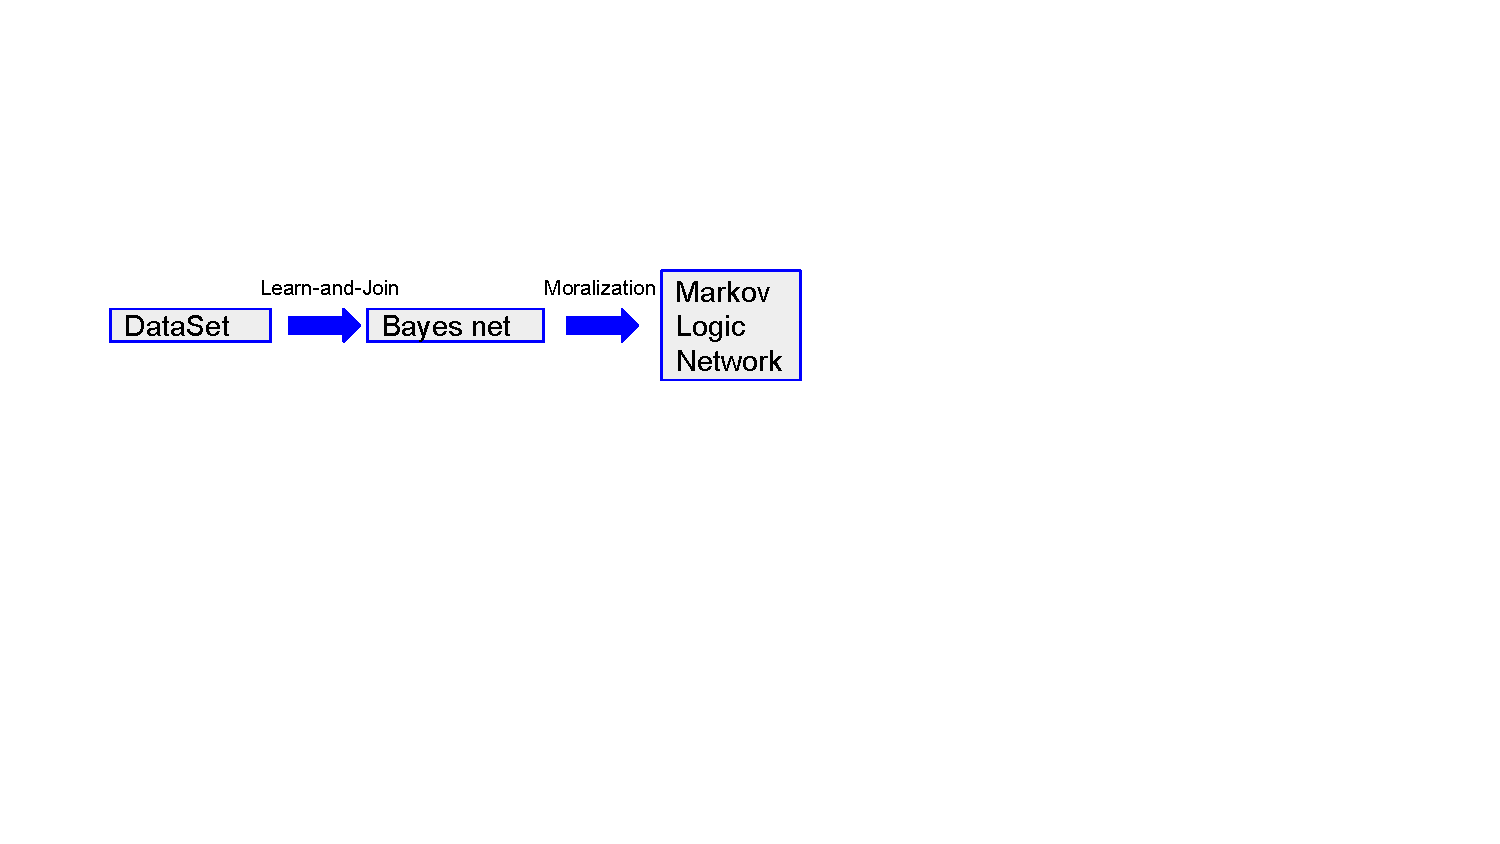
\includegraphics[width=0.8\textwidth] 
 	  		{figures/MLNLearningProcess.pdf}
 	  		\caption{Learning an Markov Logic Network from an input relational database.
 	  			%We show only the Markov blanket of the Results node to simplify. 
 	  			\label{MLNLearningProcess}
 	  		}
 	  	\end{figure}
 	 
 %	figures/MLNLearningProcess.pdf
%	 The LAJ algorithm employs an iterative deepening strategy, which can be described as as search through a lattice of table joins. For each table join, different BNs are learned and the learned edges are propagated from smaller to larger table joins. 	For a full description, complexity analysis, and learning time measurements, please see \cite{Schulte2012}. 	We used the implementation of the LAJ algorithm due to its creators \cite{bib:jbnsite}. 
 	
% 	Our emphasis is on comparing {\em learning} formulas with the baseline of {\em enumerating} all $n$-grams, so we leave for future work
% 	evaluating other MLN structure learning algorithms, such as MLN-Boost \cite{Khot2011}. 	% rather than different versions of the MLN approach. 
 	%In direct comparisons between the LAJ and the MLN-Boost systems, the classification accuracy of LAJ models has been competitive with those found by MLN-Boost~\cite{Schulte2012d}. 
 	
 	%We briefly describe the Learn-and-Join algorithm (LAJ). 
% 	The LAJ algorithm has also been employed  for MLN structure learning task. it distinguishes between descriptive attributes, such as $\it{gender(User)}$ or $\it{Rating(User,Movie)}$ and relationships, such as $\it{HasRated}(\it{User},\it{Movie})$. Relationships indicate the existence of a certain type of link between individuals. 
% 	%Attributes are properties of individuals or links. Both can be represented using  atoms. 
% 	A relationship chain is a list of relationship atoms connected by shared logical variables. 
% 	%The LAJ algorithm carries out a lattice search that performs iterative deepening with relationship chains of increasing depth. 
% 	Note that for every relationship atom, there is a set of associated descriptive attributes. For example, for the predicate $\it{HasRated}(\it{User},\it{Movie})$, the associated attributes comprise the rating, as well as the descriptive attributes of users and movies. For the initialization, for each relationship atom, the algorithm learns a set of formulas for the attributes associated with that relationship. In the implementation of \cite{Schulte2012}, a propositional graphical model learner is used to find the set of formulas. For a relationship chain of length $\ell +1$, the algorithm learns another set of formulas for the attributes associated with the relationships in the chain, with the following constraint: all formulas discovered for subchain of length $\ell$ or less are inherited by larger relationship chains. %LAJ algorithm can also be used to learn MLN structure. 
 	
 	
 	%%				
 	%%				\subsubsection{Examples} Figure~\ref{database} shows an example database. The ground literal $$(\it{ShotEff(\P,\M)} = Low) \{\P\backslash 123,\M\backslash 1\}$$$$=(\it{ShotEff}(123,1)=Low)$$ evaluates as true in this database. For the grounding count we have $$\grounds_{\D}(\it{ShotEff(\P,\M)} = Low) \{\P\textbackslash 123\}) = 2.$$
 	%%				
 	
 	%
 	%how much more general a learned rule set is if anomalous examples are omitted either by measuring the difference of the generalization of the hypotheses induced in presence or absence of the observation~\cite{Angiulli2009} or by means of satisfaction of certain conditions~\cite{Angiulli2004}. 
 	
 	
% 	\begin{figure}
% 		\centering
% 		\includegraphics[width=0.6\textwidth] {figures/OverView.pdf}
% 		\caption{System Flow
% 			\label{main:b-chapter3}}
% 	\end{figure}
% 	
 
\section{Evaluation Techniques in Outlier Detection}\label{sec:eval}
Measuring the effectiveness of outlier detection methods is not often an easy task. Most of the time ground truth information, that shows which data points are outliers, is unavailable. \\
%In this section, we first discuss how outlier detection methods in the literature have tackled this problem, then we describe how we deal with it in our research.\\ 
Several techniques have been employed in literature to evaluate the performance of outlier detection methods:
\begin{enumerate}
\item Intuitive evaluation: case studies have been extensively used in literature to evaluate outliers~\cite{aggarwal2013}. In chapter 4 we use this method of evaluation for top $n$ ranked detected outliers and we try to explain and make sense of the detected outliers. 	
\item Synthetic data generation: another approach to evaluate anomaly detection methods is generating synthetic data and inject synthetic outliers into the data~\cite{aggarwal2013}. We have designed and developed three synthetic datasets as it was discussed in section~\ref{sec:synthetic}.
\item Anomaly injection: anomalies are injected into the real-world datasets. Outlier detection methods are expected to detect the injected data points as outliers~\cite{Akoglu2015}. We employ this approach in our real world datasets.
The disadvantage of this evaluation metric is that the real world data may also contain certain type of anomalies, known as in-class outlier. However, this metric treats only the injected data points as true positive and will score anything other than those as false positive.
\item Internal Evaluation: in this type of evaluation outlier score has been used to quantify the extremity of data points~\cite{Pickands1975}.% We do not use this method of evaluation in our work.
\end{enumerate}






%% Copyright 1998 Pepe Kubon
%%
%% `one.tex' --- 1st chapter for thes-full.tex, thes-short-tex from
%%                the `csthesis' bundle
%%
%% You are allowed to distribute this file together with all files
%% mentioned in READ.ME.
%%
%% You are not allowed to modify its contents.
%%

%%%%%%%%%%%%%%%%%%%%%%%%%%%%%%%%%%%%%%%%%%%%%%%%%
%
%       Chapter 3
%
%%%%%%%%%%%%%%%%%%%%%%%%%%%%%%%%%%%%%%%%%%%%%%%%

\chapter [Propositionalization for Outlier Detection]{Propositionalization for Unsupervised Outlier Detection in Object-relational Data}\label{chap:four}

	In this chapter we develop a novel propositionalization  approach to unsupervised outlier detection for object-relational data. Propositionalization summarizes the information from relational data, that is typically stored in multiple tables, into a single data table. An advantage of propositionalization is that it facilitates leveraging the many previous outlier detection methods that were designed for single-table data. 
	Previous work has employed propositionalization for various applications; Anderson {\em et. al} ~\cite{Anderson2007} use propositionalization to apply clustering algorithms, like KMeans, to multi-relational data. Propositionalization for classification has been extensively explored~\cite{Kramer2000,Lavrac13,Lavravc2014,kuzelka2008}. ODDBALL extracts patterns from large weighted graphs and then uses those patterns as features to discover anomalous nodes in graph~\cite{Akoglu2010}.
	
	In this work we develop propositionalization for outlier detection for the case of object-relational data. 
	A novel application of Markov Logic Network structure learning is the basis of our propositionalization method for outlier detection. 
	%
	Alternative propositionalization methods that we evaluate in this work are based on enumerating all conjunctive formulas with, at most, two literals (unigrams and bigrams). 
	Compared to baseline propositionalization methods, Markov Logic propositionalization produces the most compact data tables whose attributes capture the most complex object-relational correlations. (More complex correlations are represented by longer logical formulas). We apply three representative outlier detection methods ($\lof$, $\knn$, $\outrank$) to the data tables constructed by %Markov Logic 
	propositionalization.
	%	The data tables produced by Markov Logic propositionalization capture the most complex multi-relational correlations, and were substantially more compact (half the dimensionality or less) which led to substantially faster runtimes for the outlier detection methods (twice as fast or more). 
	For each outlier detection method, Markov Logic propositionalization provided the best average accuracy over all datasets compared to the baseline propositionalization methods.
		\section{Introduction} Many outlier detection methods have been developed for data that is represented in an attribute-value format \cite{aggarwal2013}. 
		This work addresses outlier detection for object-relational data. In a single data table a row represents a data point, a column represents an attribute of a data point, and a table entry represents an attribute value for a data point. 
		%In contrast, multi-relational data are ususally represented in multiple interrelated tables. 
		Data analysis tools that are built for single data tables, can be leveraged for multiple relational data tables via a pipeline approach: first, convert the object-relational data to a single attribute-value table, then apply the data analysis tool. Since the attribute value representation corresponds to propositional logic, the conversion process is called {\em propositionalization} \cite{Kramer2000}. 
		%This paper presents a novel propositionalization method for outlier detection with multi-relational data. 
		While propositionalization for classification has been extensively explored~\cite{Kramer2000,Lavrac13,Lavravc2014,kuzelka2008}, to our knowledge propositionalization for outlier detection is a new research problem.
		
		\paragraph{Approach.} We use Markov Logic Network (MLN) structure learning to construct a single data table from object-relational data. This is a novel application of MLN learning. The format of the resulting data table is an individual-centric representation~\cite{Lippi2011,Lavrac13}:  we assume that there is a target class of individuals to be ranked as potential outliers (e.g. soccer players or movies). A row in the data table represents the attributes of an individual. Attributes are defined by logical first-order formulas~\cite{Lippi2011}. The more complex the formula, the more relational information is represented by the formula. 
		A feature function maps an individual and a first-order formula to a real value that is the value of the attribute for the individual. For example, we use the number of instantiations or groundings of a formula as such a function. 
		%
		A Markov Logic Network structure is a set of formulas.  Our Markov Logic propositionalization method applies the MLN structure learning method, introduced in chapter~\ref{chap:three}, to produce a set of formulas, these formulas define attributes for propositionalization. Our approach can be summarized by this equation:\\
		
	%	\begin{displaymath}\label{eq:formulaEssen}
			  {  \em Markov Logic Network Structure = Set of Formulas = Set of Attributes }  (4.1)\\
%		\end{displaymath}


		A baseline comparison method is to enumerate all conjunctive formulas up to a fixed length $n$ as attributes for propositionalization.  This is an instance of the recent Wordification approach to propositionalization \cite{Lavrac13}. 
		Wordification is based on an analogy between text data and relational data, where an $n$-gram in text data corresponds to a conjunctive formula with $n$ literals. In text analysis, $n$-grams are often treated as features of a document. 
		Analogously, wordification uses conjunctive formulas up to a fixed length $n$ as features for propositionalization. 
		The disadvantage of this approach is that the number of such formulas grows exponentially with $n$. 
		
		\paragraph{Evaluation.}% Our code and datasets are available on-line at \cite{url}. 
		%
		We use synthetic and real-world datasets that were introduced in chapter~\ref{chap:three}. Markov Logic propositionalization produces significantly fewer attributes, leading to much smaller  data tables for outlier analysis compared to the baseline wordification approach. The MLN attributes capture more complex relational associations 
		% (half the number of columns or less). 
		(with over 3 literals on average compared to 2 literals for wordification). 
		%Using the $\auc$ accuracy metric,
		%, which is standard for outlier detection, 
		MLN propositionalization is competitive with wordification: for a given outlier analysis method,~%(one of $\lof$, $\knn$, $\outrank$), 
		the average $\auc$ score over all datasets is best for MLN propositionalization.
		
		We believe that propositionalization for outlier detection is a fruitful application area for other statistical-relational learning generative models in addition to Markov Logic Networks. 
		Our approach can  utilize %structure learning for 
		any model class whose structure is represented by logical formulas, or can be easily converted to logical formulas, which includes many statistical-relational models~\cite{Ravkic2015,Cussens2012,Kersting2007,SRL2007}.
		
		\paragraph{Contributions.} The contributions of this chapter may be summarized as follows. 
		
		\begin{enumerate}
			\item A novel task for relational learning: propositionalization for outlier detection. This facilitates leveraging standard single-table outlier analysis methods for object-relational data.
			\item A novel application of Markov Logic Network structure learning to perform this task. MLN structure learning generates a compact yet expressive set of features from object-relational data.
		\end{enumerate}
%			\section{Related Work} 
%			\paragraph{Propositionalization} 
%			has been explored extensively for classification tasks \cite{Kramer2000,Lavrac13,Lavravc2014,kuzelka2008}. We are not aware of previous work on propositionalization for {\em outlier detection.}  The wordification framework \cite{Lavrac13} introduces an analogy between the grounding counts of a formula and the frequency of a term in a document. Lavrac {\em et al.} apply this analogy for propositionalization for classifiers, which is implemented in the ClowdFlows system~\cite{Kranjc2012}. The $n$-gram methods in this chapter apply the analogy for outlier detection. 
%			
%			In previous applications of single-table outlier analysis methods to structured data, the data were manually propositionalized, by aggregating information about single attributes. 
%			For example, Breunig {\em et al.} counted the total number of goals scored by a player in a season as a attribute for outlier analysis by $\lof$\cite{Breunig2000}. Counts for single attributes in isolation are basically equivalent to the unigram-term frequency method that we evaluate in our experiments. Manual propositionalization is limited because it becomes very difficult for attributes that represent interactions between features (e.g., the bigram method below).
%			
%			
%			\paragraph{Relational Outlier Detection} has previously been based on discovering rules that represent the presence of anomalous associations for an individual or the absence of normal associations \cite{Novak2009,Maervoet2012}. 
%			%	Several deviation measures have been proposed for association rules \cite{Novak2009}.
%			Related work includes exception mining, which looks for associations that characterize unusual cases, subgroup mining, which looks for associations  characterizing important subgroups, and contrast space mining, which looks for differences between classes.  Novak {\em et al.}~\cite{Novak2009} show that these tasks can be unified as instantiations of a general rule search framework. None of the rule search methods use propositionalization. We were not able to obtain rule search implementation code for empirical comparison. 
%			
%			The community distribution approach \cite{Gupta2013} assumes a vector for each entity that indicates membership probabilities in different communities. Outliers can then be defined similar to the non-relational feature vector setting. Markov Logic propositionalization utilizes information from entities and links of different types, but does not assume that latent communities have been identified. 
%			
%						\paragraph{Inductive Logic Programming} has been used for relational outlier detection. One approach views an example as anomalous if it is not covered by a learned set of rules \cite{Angiulli2007}. Another measures the difference in generality between a rule set learned with the anomalous examples, and a rule set learned without ~\cite{Angiulli2009}. Neither performs propositionalization. No code is available for empirical comparison.
%%				
%				\section{Background and Notation} 
%				
%				We use notation and terminology from previous work \cite{Chiang2012,Lippi2011,Domingos2009}. While we do not introduce any new terminology, we combine concepts from different areas, such as propositionalization and log-linear models. We follow the description of propositionalization in Lippi {\em et al.} \cite{Lippi2011}, where the input to a propositionalizer is a relational database, and the output is a pseudo-\iid data view. 
%				
%%				\subsection{Predicate Language}
%%				
%%				We employ the notation of Chiang and Poole \cite{Chiang2012} for logical syntax, as follows.
%%				%
%%				Constants are expressed in lower-case, e.g. $\it{joe}$, and are used to represent individuals. A type is associated with each individual, e.g. $\it{joe}$ is a person. We use $D(\tau)$ to represent a domain of type $\tau$, which is the set of individuals of type $\tau$. A {\em logical variable} is written in upper case. A logical variable is also typed, e.g. $\it{Person}$ denotes some member of $D(\tau)$. A relation is given by 
%%				$$r : \Omega \rightarrow V_{r}$$
%%				where $r$ is the name of the relation, $\Omega_{r}=D(\tau_{1})\times \ldots \times D(\tau_{a})$ is the domain of the relation, and $T_{r}=(\tau_{1},\ldots,\tau_{a})$ is the type of the relation. $V_{r}={v_{1},\ldots,v_{k}}$ is the range of the relation. Number $a$ and $k$ are positive integers denoting the {\em arity} and {\em size} of $r$. An {\em atom} is an expression of the form $r(\sigma_{1},\ldots,\sigma_{a})$ where each $\sigma_{i}$ is either a constant or logical variable. If all of $\sigma_{1},\ldots,\sigma_{a}$ are constants, $r(\sigma_{1},\ldots,\sigma_{a})$ is a {\em ground atom}.
%%				
%%				A {\em literal} specifies the value of an atom e.g. $r(X_{1},\ldots,X_{a})=v$ where $v \in V_{r}$. A literal is also a {\em formula}. Formulae with multiple literals are formed using connectives $\wedge$ and or $\vee$. Connecting literals using only $\wedge$ forms a {\em conjunctive formula } or {\em conjunction}. A formula that contains no logical variables is a {\em ground} formula.
%%				%, is a proposition.
%%				%A {\em disjunctive formula} or {\em disjunction} is formed using only $\vee$. \\
%%				
%%				A substitution is a set $\{X_{1} \textbackslash x_{1}, \ldots, X_{k}\textbackslash x_{k}\}$ where $X_{i}$ are distinct logical variables and $x_{i}$ are constants. When applied to a formula $f$, each occurrence of $X_{i}$ in $f$ is replaced with $x_{i}$. We denote the application of a substitution 
%%				%$\{X_{1} \textbackslash x_{1}, \ldots, X_{k}\textbackslash x_{k}\}$ 
%%				to $f$ as $f\{X_{1} \textbackslash x_{1}, \ldots, X_{k}\textbackslash x_{k}\}$. 
%%				Consider a formula $f$ containing logical variables $X_{1}, \ldots,X_{n}$, where each $X_{i}$ has type $\tau_{i}$. The {\em grounding space} of $f$, is the set of all possible grounding substitutions for $f$, given by 
%%				$$\{\{X_{1}\textbackslash x_{1}, \ldots, X_{n}\textbackslash x_{n}\}:x_{i} \in D(\tau_{i}) \mbox{ for } i=1,\ldots,n\}.$$
%%				
%%				%	Given some formula $f$ containing logical variables $X_{1}, \ldots,X_{n}$, where each $X_{i}$ has type $\tau_{i}$, let the domain of $f$ be $\Omega_{f}=D(\tau_{i}\times \tau_{n})$. The {\em substitution space} of $f$, $\Gamma_{f}$, is the set of all possible grounding substitutions for $f$, given by 
%%				%	$$\Gamma_{f}=\{\{X_{1}\textbackslash x_{1}, \ldots, X_{n}\textbackslash x_{n}\}:(x_{1},\ldots,x_{n})\in \Omega_{f}\}.$$
%%				
%%				A \emph{database} $\D$ specifies for each ground literal whether the literal is true in the database or not. A ground conjunction is true in a database if all of its conjuncts are true. The \emph{count} of groundings satisfying formula $\formula$ with respect to a database $\D$ is denoted as $\grounds_{\D}(\formula)$.
%%				
%					\subsection{Logical Concepts}
%					We adopt a term-based notation for logical concepts~\cite{Poole2003,Chiang2012}. Constants such as $\it{rooney}$, $123$ are used to represent individuals. A \textbf{population} is a set of individuals. 
%					A functor is a function or predicate symbol, denoting a function that is applied to individuals. Each functor has a set of possible values (constants) called the \textbf{domain} of the functor. The domain of a \textbf{predicate} is $\{\true,\false\}$. Predicates are usually written with uppercase Roman letters, other terms with lowercase letters.
%					A predicate of arity at least two is a \textbf{relationship} functor. Relationship functors specify which objects are linked. Other functors represent \textbf{features} or \textbf{attributes} of an object or a tuple of objects (i.e., of a relationship).
%					A \textbf{term} is of the form $f(\term_{1},\ldots,\term_{k})$ where $\functor$ is a functor %(either a function symbol or a predicate symbol) 
%					and each $\term_{i}$ is a first-order variable or a constant. 
%					An {\em atomic assignment} specifies the value of a term e.g. $\functor(\term_{1},\ldots,\term_{k})=v$ where $v$ is in the domain of functor $\functor$. 
%					%A literal is also a {\em formula}. 
%					%		Formulae with multiple literals are formed using connectives $\wedge$ and or $\vee$. 
%					Connecting assignments using only $\wedge$ forms a {\em conjunctive formula } or {\em conjunction}. In this paper we use conjunctive formulas only. A term/literal/formula is \textbf{ground} if it contains no first-order variables; otherwise it is a first-order term/literal/formula. 
%					
%					An object-relational database $\D$ specifies the values of all ground terms, and hence whether a ground literal is true or not. A ground conjunction is true in a database if all of its conjuncts are true. A \textbf{grounding} is a set $\{X_{1} \backslash x_{1}, \ldots, X_{k}\backslash x_{k}\}$ where $X_{i}$ are distinct logical variables and $x_{i}$ are constants. When applied to a formula, each occurrence of $X_{i}$ is replaced with $x_{i}$. 
%					%We denote the application of a substitution 
%					%$\{X_{1} \backslash x_{1}, \ldots, X_{k}\backslash x_{k}\}$ 
%					%		to $f$ as $f\{X_{1} \backslash x_{1}, \ldots, X_{k}\backslash x_{k}\}$.
%					%		
%					The \textbf{count} of groundings that satisfy (make true) formula $\formula$ with respect to a database $\D$ is denoted as $\grounds_{\D}(\formula)$.	
%					
%					
%					\subsubsection{Markov Logic Networks} A Markov Logic Network (MLN) \cite{Domingos2009} is a set $\{(\formula_{1},\w_{1}),\ldots,(\formula_{\numformulas},\w_{\numformulas})\}$ where $\formula_{i}$ is a formula, and each $\w_{i}$ is a real number called the weight of $\formula_{i}$. The MLN semantics views a formula with logical variables as a feature template that is instantiated by ground formulas. The number $\numformulas$ of formulas is independent of the size of the instantiated MLN.
%					The log-linear likelihood of a possible world/database is proportional to the weighted sum, over all formulas, of the grounding count of each formula in the given database:
%					\begin{equation} \label{eq:mln} P(D) \propto \exp(\sum_{i=1}^{\numformulas} \w_{i} \cdot \grounds_{\D}(\formula_{i}))\end{equation}
%					
%					This semantics defines a joint distribution over descriptive attributes of entities, links between entities, and attributes of those links. \cite{Domingos2009} discuss the representational power of this semantics.
%					
%%%				
%%%				\subsubsection{Examples} Figure~\ref{database} shows an example database. The ground literal $$(\it{ShotEff(\P,\M)} = Low) \{\P\backslash 123,\M\backslash 1\}$$$$=(\it{ShotEff}(123,1)=Low)$$ evaluates as true in this database. For the grounding count we have $$\grounds_{\D}(\it{ShotEff(\P,\M)} = Low) \{\P\textbackslash 123\}) = 2.$$
%%%				
%
%			%
%			%how much more general a learned rule set is if anomalous examples are omitted either by measuring the difference of the generalization of the hypotheses induced in presence or absence of the observation~\cite{Angiulli2009} or by means of satisfaction of certain conditions~\cite{Angiulli2004}. 
%				\subsubsection{Examples} Figure~\ref{main:a} shows an example database. The ground literal $$(\it{ShotEff(\P,\M)} = Low) \{\P\textbackslash 123,\M\textbackslash 1\}=(\it{ShotEff}(123,1)=Low)$$ evaluates as true in this database. For the grounding count we have $$\grounds_{\D}(\it{ShotEff(\P,\M)} = Low) \{\P\textbackslash 123\}) = 2.$$
%				
%						\begin{figure}
%							\centering
%							\includegraphics[width=0.6\textwidth] {figures/databasefigure.pdf}
%							\caption{An example database
%								\label{main:a}}
%						\end{figure}
						
									\begin{figure}
										\centering
										\includegraphics[width=0.6\textwidth] {figures/OverView.pdf}
										\caption{System Flow
											\label{main:b-chapter3}}
									\end{figure}
									
				
			%	\begin{figure}[!htbp]
%					
%					\begin{minipage}{.5\linewidth}
%						\centering
%						\subfloat[An example database]{\label{main:a}\includegraphics[scale=.6]{databasefigure.pdf}}
%					\end{minipage}%
%					\begin{minipage}{.55\linewidth}
%						\centering
%						\subfloat[The Propositionalization Pipeline]{\label{main:b}\includegraphics[scale=.45]{OverView.pdf}}
%					\end{minipage}\par\medskip
%					\caption{System Flow}
%					\label{fig:propositionalize}
%				\end{figure}
				

\section{Propositionalization, Pseudo-\iid data views, and Markov Logic Networks} Figure~\ref{main:b-chapter3} provides an overview of our propositionalization system. Lippe {\em et al.} \cite{Lippi2011} describe propositionalization in terms of a pseudo-\iid (p-\iid) data view. A p-\iid data view is a data table in which one row specifies attribute values for one example. Statistical analysis tools, such as outlier analysis methods, that take as input single-table data are applied to the p-\iid data view. 
%The data table is then used in place of a data table that represents \iid datapoints. 
Since in the relational case the attribute values in different rows are often not independent, Lippi {\em et al.} coined the term ``pseudo-\iid''. 
%To describe pseudo-iid views, we need some concepts from logic; 
%Types are assumed disjoint. 

%\subsubsection{Example of Relational Database}




%	\setlength{\tabcolsep}{.16667em}
\begin{table*}
	
	\centering
	\caption{An example pseudo-iid data view. For definitions please see text.
		\label{table:Features}}
	\resizebox{1\textwidth}{!}{
		
		\begin{tabular}{|l|c|c|c|c|}
			\hline
			%Formula&\multicolumn{2}{|c|}{\begin{tabular}{p{5cm}} $1/2 \log(0.5/0.5)=0 $\end{tabular}}\multicolumn{2}{|c|}{F2 Vector}\\\hline
			Formula $\rightarrow$&\multicolumn{2}{|c|}{\begin{minipage}{13cm}\begin{equation} SavesMade(P,M)=med\wedge shotsOnTarget(P,M)=lo\wedge \it{\it{ShotEff}}(P,M)=lo \nonumber\end{equation}\end{minipage}}&\multicolumn{2}{|c|}{\begin{minipage}{13cm}\begin{equation}SavesMade(P,M)=med\wedge shotsOnTarget(P,M)=hi\wedge \it{ShotEff}(P,M)=hi \nonumber\end{equation}\end{minipage}}\\\hline
			\begin{tabular}{p{3cm}} Feature Function $\rightarrow$\\ Player $\downarrow$ \end{tabular}&\begin{tabular}{p{4cm}}\hspace{1.5cm} \tf \end{tabular}&\begin{tabular}{p{4cm}}\hspace{1.3cm} \tfidf\end{tabular}&\begin{tabular}{p{4cm}}\hspace{1.5cm}\tf \end{tabular}&\begin{tabular}{p{4cm}}\hspace{1.3cm}\tfidf \end{tabular} \\\hline
			Wayne Rooney &4&1.99&12&33.83\\\hline
			David Silva&6&2.99&19&53.57\\\hline
			Robin VanPersie&2&0.99&24&67.67\\\hline
		\end{tabular}
	}
	
\end{table*}
%\begin{minipage}{15cm}\begin{equation} $SavesMade(P,M)=med\wedge shotsOnTarget(P,M)=lo\wedge \it{\it{ShotEff}}(P,M)=lo$ \nonumber\end{equation}\end{minipage}
\begin{definition}[based on \cite{Lippi2011}]
	Let $\D$ be a relational database. A pseudo-\iid (p-\iid) data view of $\D$ comprises 
	
	\begin{enumerate}
		\item a logical variable $\examplevar$, called the \textbf{example variable}
		\item a set of examples, where each example consists of a constant in the domain of $\examplevar$
		\item a set of \textbf{attributes} $\ffunction_{1},\ffunction_{2},\ldots,\ffunction_{d}$. An attribute specifies a real number given an example and the database $\D$. 
		%In the terminology of log-linear models \cite{Sutton2007,Taskar2002,Domingos2009}, attributes correspond to \textbf{feature functions}. 
	\end{enumerate}
\end{definition}

Lippi {\em et al.} give a more general definition of p-\iid views where examples may consist of tuples rather than a single constant. In our experiments we used only single individual examples (=constants). In the framework of Lippi {\em et al.}, an attribute is derived from two components. (1) A conjunctive formula, called a query. The formula can be viewed as a {\em template} that can be instantiated multiple times for a single example. (2) A function that aggregates the multiple instantiations to derive a real number that is the value of the attribute. Lippi {\em et al.} introduce two basic feature functions: the instantiation count (how many times the query formula is instantiated) and existence, a 0/1-valued attribute that indicates whether there is some instantiation of the feature for the given individual. 
\paragraph{Propositionalization via Markov Logic Networks.}



%Figure~\ref{main:b-chapter3} provides an overview of our propositionalization system. 
 Propositionalization is usually applied as a technique for {\em discriminative} learning in relational data \cite{Kramer2000}. A new idea in this work is that pseudo-\iid data views can also be derived from {\em generative} models. The generative model we employ is Markov Logic Networks \cite{Domingos2009}. Markov Logic Network learning provides a way to learn formulas for constructing pseudo-\iid views, we refer to this as {\em MLN propositionalization}.
% The output of the propositionalizer as a \textbf{pseudo-\iid data view}, because the data matrix is processed by methods designed for i.i.d. data, even though the relational structure induces dependencies between rows in the data matrix. Each column (attribute) of the pseudo-iid data view is associated with a conjunctive formula called the query. The query contains a logical \textbf{example variable} $\E$. For instance, if we are interested in detecting anomalous players, $\it{Player}$ is an appropriate example variable.
For each example individual, the value of an attribute  is determined by a feature function that aggregates the multiple instantiations of the attribute query for the individual in order to derive a real number.% In the terminology of log-linear models like MLNs, such functions are called \textbf{feature functions}~\cite{Domingos2009}. 
%One feature function considered by Lippi {\em et al.} is the instantiation count (how many times the query is instantiated). 
 %Table~\ref{table:Features} illustrates feature functions. In sum, pseudo-\iid data views are constructed as follows\begin{}
% 	
\begin{quote}
	Formula + Feature Function = Attribute Values
\end{quote}








%MLN structure learning constructs a set of formulas for a given input database. In this work, we propose a novel application of MLN structure learning for outlier detection: {\em use the formulas discovered by structure learning to define attributes in a pseudo-\iid view}; see Figure~\ref{main:b-chapter3}. For each formula in the MLN, the instantiation count is  the value of the attribute corresponding to that formula. Table~\ref{table:Features} presents an example of some attributes defined by MLN formulas. In principle, this propositionalization method can employ any MLN structure learning algorithm. 	
The motivation for Markov Logic propositionalization is as follows.
	
	\begin{enumerate}
		\item Constructing a generative model is one of the major approaches to unsupervised outlier detection~\cite{aggarwal2013}. Intuitively, the generative model represents normal behavior in the population. 
		\item The formulas in the MLN indicate which relations are normally associated and which are normally independent of each other. 
		\item Relevant formulas are learned from the data, rather than constructed from a fixed a priori set of templates.
		%\item Learning relevant formulas has two advantages over exhaustively constructing all formulas
		%%$n$-grams 
		%of a fixed length:
		%\begin{enumerate}
		%\item dimensionality reduction: we learn a more compact set of formulas, which translates into a smaller set of attributes (columns) in the pseudo-\iid data view. 
		%\item It is possible to learn formulas for arbitrary length. 
		%\end{enumerate}
	\end{enumerate}
	
	
	%Lippi {\em et al.} introduce two basic feature functions: the feature count (how many times the template is instantiated) and existence, a 0/1-valued attribute that indicates whether there is some instantiation of the feature for the given individual. 
	
	Algorithm~\ref{alg:propositionalize} describes how this propositionalization schema can be applied with Markov Logic Networks. 
	%The output of the algorithm is a data matrix. The number of rows is the number of individuals in the domain of the example variable. The number of columns is the number of formulas in the input MLN. 
%	This schema requires the specification of a feature function, which we discuss next.
\begin{algorithm}[htb]
	\begin{algorithmic}
		{\footnotesize
			\STATE {\em Input}: An MLN $\{(\formula_{1},\w_{1}),\ldots,(\formula_{\numformulas},\w_{\numformulas})\}$; Database $\D$; Example logical variable $\E$.
			\STATE {\em Output}: A data matrix $D$. (Pseudo-iid data view.)
			\STATE {\em Calls}: Feature Function $\ffunction$. $\ffunction(\a,\formula,\D)$ returns a number.
		} %fnsize
	\end{algorithmic}
	\begin{algorithmic}[1]
		{\footnotesize
			\STATE For each individual $a_{1},\ldots,a_{n}$ in the domain of the example variable $\E$, add a \textbf{row} to the data matrix $D$.
			\STATE For each formula $\formula_{1},\ldots,\formula_{\numformulas}$ in the MLN that contains the example variable, add a \textbf{column} to the data matrix $D$.
			\FORALL{individuals $a_{i}$ and formulas $\phi_{j}$}
			\STATE $D_{ij} := \ffunction(a_{i},\phi_{j},\D)$.
			\ENDFOR
			\STATE Return $D$.
			%\FORALL [A relationship node is a parent of a Entity node]{dependencies of kind $X(R_m) \rightarrow Y(E_i)$}
			%	%\IF {dependency is of kind $X(R_m) \rightarrow Y(E_i)$ } 
			%	\STATE add $R_m \rightarrow Y(E_i)$ to $G$
			%	\ENDFOR	
			%\STATE Run dynamic programing algorithm
		} %footnotesize
	\end{algorithmic}
	%\label{alg:cpt}
	\caption{Markov Logic Network Propositionalization\label{alg:propositionalize}}
\end{algorithm}	
	
	%\subsection{Structure Learning for Markov Logic Networks}
	
	
	
	
	\section{Wordification: $n$-gram Methods}
	
	As a baseline for empirical comparison, we present an alternative approach to generating formulas in a pseudo-\iid view based on the wordification analogy between relational and text data that is introduced by Lavrac {\em et al.}~\cite{Lavrac13}. 
	The wordification analogy is as follows:
	
	\begin{itemize}
		\item A document corresponds to an example individual. 
		\item A  word in a document corresponds to a literal.
		\item An $n$-gram in a document (i.e., a sequence of $n$ words) corresponds to a conjunction of $n$ literals. In our datasets this was computationally feasible for $n<3$.
		\item The term frequency (TF) of an $n$-gram in  a document corresponds to the conjunction grounding count.
	\end{itemize}
	
	Just as a formula can have multiple groundings for an individual in a database, an $n$-gram can occur multiple times in a document.
	The wordification analogy suggests using the analog of $n$-grams in text mining. 
	%For instance, a unigram is a literal containing the example variable $\examplevar$. A bigram is a conjunction of two literals that share at least one first-order variable, and such that the example variable appears in the conjunction. [Sarah: how about we use wordification as a baseline?]
	%The instantiation count corresponds to term frequency (TF) in a document. 
	A range of functions for defining attribute values have been explored in NLP research; perhaps the most widely used is term frequency/inverse document frequency ($\tfidf$), which down-weights terms that are frequent across documents~\cite{Lavrac13}.  The two feature functions we employ in this paper are analogs of TF and $\tfidf$.  %The $\tfidf$ of a formula is defined as follows.
	For a given $w$ in document $d$ from corpus $D$, the $\tfidf$ measure is defined as follows:
	
	\begin{equation}
	\tfidf(w,d)=\tf(w,d)\times log\frac{|D|}{{d\in D : w \in d}}
	\end{equation}
	In sum, we use the following methods for generating formulas in a p-\iid data view. All generated formulas are constrained to contain the example variable. 
	
	\begin{description}
		\item[MLN] Learn a Markov Logic Network for the given database, then use the learned formulas.
		\item[Unigram]  All single literals.
		\item[Bigram] All conjunctions of two literals that share at least one first-order variable.
	\end{description}
	
 
	%~\cite{Sutton2007,Taskar2002,Domingos2009}. 
	%The log-likelihood of a possible world or database is proportional to the weighted sum of feature functions. 
	%In MLNs, the feature function used is the feature count. In this paper, we consider other feature functions as well for unsupervised anomaly detection. 
%	Using this terminology, the construction of attributes in a p-\iid data view can be summed up as follows:
%	
%	\begin{quote}
%		Formula + Feature Function = Attribute Values
%	\end{quote}
	
	Combining our three formula generating methods with two feature functions defines a space of six methods for constructing a p-\iid data view for outlier detection, as illustrated in Table~\ref{table:methods}. Table~\ref{table:Features} presents an example of a pseudo-\iid view with two trigram formulas learned from data and attribute values computed from the real-world data. 
	\begin{table*}
		
		\centering
		\caption{Generating pseudo-\iid data views using Feature Functions and Formulas
			\label{table:methods}}
		\resizebox{0.7\textwidth}{!}{
			\begin{tabular}{|c|c|c|}
				\hline
				
				\begin{tabular}{p{3cm}}Feature Function $\rightarrow$\\ Formula $\downarrow$ \end{tabular}&\begin{tabular}{p{1cm}}\tf\end{tabular}&\begin{tabular}{p{2cm}}\tfidf\end{tabular}\\\hline
				Unigram&Unigram-TF&Unigram-IDF\\\hline
				Bigram&Bigram-TF&Bigram-IDF\\\hline
				MLN&MLN-TF&MLN-IDF\\\hline
			\end{tabular}
		}
		
	\end{table*}
	\section{Experimental Design: Methods Used}
	
	We evaluate the  six methods shown in Table~\ref{table:methods}. The Unigram-IDF approach produced substantially weaker results than Unigram-TF on all datasets, so we omit this method to simplify the presentation.
	%
	Generating unigrams and bigrams is straightforward given a predicate language. Instantiation counts for term frequencies and inverse document frequencies were computed using MySQL Server version 5.5.34.. The most complex computation is structure learning for MLNs. We use a previously existing algorithm that we briefly review.
	
	\paragraph{MLN Structure Learning.} In principle, our propositionalization method can employ any MLN structure learning algorithm. In this work we employ the Learn-and-Join (LAJ) algorithm that was discussed in chapter~\ref{chap:three}. This is a state-of-the-art MLN structure learning algorithm, especially well-suited for datasets with many descriptive attributes such as those in our empirical evaluation \cite{Khosravi2010,Schulte2012}. Our emphasis is on comparing {\em learning} formulas with the baseline of {\em enumerating} all $n$-grams, so we leave 
	evaluating other MLN structure learning algorithms, such as MLN-Boost \cite{Khot2011}, for future work. 	% rather than different versions of the MLN approach. 
	%In direct comparisons between the LAJ and the MLN-Boost systems, the classification accuracy of LAJ models has been competitive with those found by MLN-Boost~\cite{Schulte2012d}. 
	
	%We briefly describe the Learn-and-Join algorithm (LAJ). 
%	The LAJ algorithm distinguishes between descriptive attributes, such as $\it{gender(User)}$ or $\it{Rating(User,Movie)}$ and relationships, such as\\ $\it{HasRated}(\it{User},\it{Movie})$. Relationships indicate the existence of a certain type of link between individuals. 
%	%Attributes are properties of individuals or links. Both can be represented using  atoms. 
%	A relationship chain is a list of relationship atoms connected by shared logical variables. 
%	The LAJ algorithm carries out a lattice search that performs iterative deepening with relationship chains of increasing depth. Note that for every relationship atom, there is a set of associated descriptive attributes. For example, for the predicate $\it{HasRated}(\it{User},\it{Movie})$, the associated attributes comprise the rating, as well as the descriptive attributes of users and movies. For the initialization, for each relationship atom, the algorithm learns a set of formulas for the attributes associated with that relationship. In the implementation of \cite{Schulte2012}, a propositional graphical model learner is used to find the set of formulas. For a relationship chain of length $\ell +1$, the algorithm learns another set of formulas for the attributes associated with the relationships in the chain, with the following constraint: all formulas discovered for subchain of length $\ell$ or less are inherited by larger relationship chains.
	
	\paragraph{Outlier Analysis Methods.}
	
	
	We applied the following three standard matrix-based outlier analysis methods to the pseudo-\iid data views: $\lof$, $\knn$ and $\outrank$. These methods have been explained in details in chapter~\ref{chap:two}.
	
	
%								\begin{description}
%									\item[$\lof$] is a standard density-based method~\cite{Breunig2000}.
%									It quantify the outlier-ness of the data points relative to regions of different densities. Therefore, the score is defined based on local density instead of the nearest neighbor distance. In simple words, 
%									$\lof$ compares the density of area around an object to the densities of the areas of the surrounding objects. 
%									However, $\lof$ defines density as the inverse of the average of the smoothed reachability distances in a neighborhood and this definition is not the precise definition of density in terms of number of data points within a specific region. $\lof$ is only sensitive to the density of the area and  ignore the orientation and the shape of the area.
%									\item[$\knn$] is a well-known distanced-based outlier ranking method that assigns a score to each data point on the basis of distance of the point from its $k^{th}$ nearest neighbor ($D^k$) and  declare the top $n$ points as outliers~\cite{Ramaswamy2000}. 
%									They introduce a {\em partition-based} algorithm to set a upper bound and lower bound on $D^k$ to identify the partitions that cannot contain the top $n$ outliers and prune them in order to limit the search space. % \textbf{Sarah:more precise please}
%									\item[$\outrank$] employs subspace analysis to measure the degree of outlierness. It compares clusters in different subspace to derive an outlier score for each object. This method has been explain in more details in Chapter~\ref{chap:two}.
%									
									
%									
%									\begin{figure*}[htbp]
%										\centering
%										\resizebox{0.45\textwidth}{!}{
%											\includegraphics%[width=0.3\textwidth] 
%											{figures/lof-pic.pdf}
%										}
%										\caption{ Point A has a high LOF score because its density is lower than its neighbours densities. Dotted circles show the distance to each point's third nearest neighbour.
%											%Correlations are the same, but the single feature distributions are not.
%											\label{fig:lof}}
%									\end{figure*}
						%		\end{description}
								
					

								
%								Density and distance based methods are two fundamental approaches to outlier detection represented in our study by $\lof$ and $\knn$. The $\outrank$ research of~\cite{Muller2012} suggests that \textit{PRO-CLUS} is the best clustering function for their approach. Our experiments applied $\outrank$ with two subspace clustering models, \textit{PRO-CLUS} \cite{Muller2012} and \textit{DISH} \cite{Kriegel2007}.  
%								We used the available implementation of all three data matrix methods from the state of the art data mining software \textit{ELKI} \cite{Elke2013}. 
	
	These methods represent three fundamental approaches to outlier detection. 
	%Subspace analysis is a popular approach too, and relevant to our study because $\mid$ is sensitive to correlations among attributes as well. 
	Both $\lof$ and $\knn$ require specifying the value of a $k$ parameter. Following the recommendation of the $\lof$ creators~\cite{Breunig2000}, we employed the three $k$-values 10, 15, 20. Our experiments report the best results.
	The $\outrank$ research suggests using  \textit{DISH} or \textit{PRO-CLUS} as clustering subroutines~\cite{Muller2012}. Our experiments applied \textit{DISH} \cite{Kriegel2007}. Outrank requires three parameters to be specified: $\alpha$, $\epsilon$ and $\mu$. For these parameters we tested different values in the suggested range  and the experiments report the best results. 
	We used the available implementation of all three data matrix methods from the state-of-the-art data mining software \textit{ELKI}~\cite{Elke2013}. 
	\section{Evaluation Results}
	\subsection{Performance Metrics Used}
	We report several properties of the pseudo-\iid data views produced by the different methods. 
	\begin{description}
		\item[Dimensionality] The number of attributes in the pseudo-\iid data view.
		\item[Attribute Complexity] The length of the conjunctions that define the attributes.
		\item[Outlier Analysis Run Time] How long it takes each outlier method to rank outliers, given the pseudo-\iid data view.
		\item[Attribute Construction Time] How long it takes to build the pseudo-\iid view from an input relational database. 
	\end{description}
	
	
	Our performance accuracy score for outlier rankings is the area under curve ($\auc$) of the well-established receiver operating characteristic $\roc$ curve. 
	This has been widely used to measure the performance of outlier ranking methods~\cite{Muller2012}. The relationship between false positive rate (1- Specificity) and true positive rate (Sensitivity) is captured by the $\roc$ curve. Ideally, the best performance is achieved when we have the highest sensitivity and the highest specificity. 
	%The area under the \textit{ROC} curve shows the overall performance and it is a measure to compare the curves numerically. 
	The maximum values for $\auc$ is 1.0, indicating a perfect ranking with 100\% sensitivity and 100\% specificity. In order to compute the $\auc$ value, we used the \textit{R} package \textit{ROCR}~\cite{RROCR2012}. Given a set of outlier scores, one for each object, this package returns an $\auc$ value. 
	
	
	The summary of our findings is that MLN propositionalization shows the following advantages and disadvantages. The details follow.
	
	\begin{itemize}
		\item For a fixed outlier detection method, competitive accuracy over all datasets (the best for $\lof$ and $\knn$ tie with Bigram-idf for $\outrank$). 
		\item Compact pseudo-\iid data views: substantially fewer attributes (columns) than bigrams, yet average formula length 3.27 or greater.
		\item Faster outlier analysis due to this compactness.
		\item There is learning overhead for discovering relevant formulas, but it is small (e.g. 5 minutes for MLN learning vs. 1 minute for bigram construction).
	\end{itemize}
	
	
	\subsection{Dimensionality of Pseudo-\iid Data Views}
	
	Figure~\ref{fig:dimensionality} provides information about the formulas constructed by the different propositionalization methods and the size of the resulting data table. For unigram resp. bigram methods, the formulas have length 1 resp. 2 by definition. The average formula length for MLNs is above 3 for the soccer data, for the IMDb data above 4. This shows that MLN structure learning finds more complex formulas beyond length 2. For the dimensionality of the resulting pseudo-\iid views, there is a big increase from unigrams to bigrams (e.g. from 63 to 1825 for Strikers vs. Goalies). The dimensionality of MLN pseudo-\iid data views lies between that of  unigrams and bigrams (e.g. 331 for Strikers vs. Goalies). This shows that MLN structure learning can find complex longer formulas with a relatively small increase in the dimensionality of the resulting pseudo-\iid data view, compared to bigrams. The trade-off is that learning a compact set of relevant formulas takes more time than enumerating all formulas up to a fixed length. However, the learning overhead is small (e.g. 5.24 min vs. 1.2  min for Strikers vs. Goalies). The smaller dimensionality can decrease the running time of the outlier detection methods, as shown in Table~\ref{table:outrank-time}. For example, the running time of the Outrank method for Strikers vs. Goalies is 861,870 ms given the Bigram $\tfidf$ data view, vs. 64,837 for the MLN $\tfidf$ data view. For the other two outlier detection methods the run-time difference was negligible.
%	\begin{table*}
%		
%		\centering
%		\caption{Comparison of complexity, dimensionality and construction time for the attributes produced by different propositionalization methods. \label{table:dimensionality}}
%		\resizebox{1\textwidth}{!}{
%			\begin{tabular}{|l|c|c|c|c|c|c|c|c|c|}
%				\hline
%				%Formula&\multicolumn{2}{|c|}{\begin{tabular}{p{5cm}} $1/2 \log(0.5/0.5)=0 $\end{tabular}}\multicolumn{2}{|c|}{F2 Vector}\\\hline
%				Formula&\multicolumn{3}{|c|}{\begin{tabular}{p{2cm}}MLN \end{tabular}}&\multicolumn{3}{|c|}{\begin{tabular}{p{2cm}}Bigram\end{tabular}}&\multicolumn{3}{|c|}{\begin{tabular}{p{2 cm}}Unigram\end{tabular}}\\\hline
%				\begin{tabular}{p{2cm}}Dataset$\downarrow$\end{tabular}&\begin{tabular}{p{2cm}}$\mu$(Formula\\ Length) \end{tabular}&Dimensionality&
%				\begin{tabular}{p{2cm}}	Construction\\ Time(min)\end{tabular}&\begin{tabular}{p{2cm}}$\mu$(Formula\\ Length) \end{tabular}&Dimensionality&
%				\begin{tabular}{p{2cm}}	Construction\\ Time(min)\end{tabular}&\begin{tabular}{p{2cm}}$\mu$(Formula\\ Length) \end{tabular}&Dimensionality&
%				\begin{tabular}{p{2cm}}	Construction\\ Time(min)\end{tabular}\\\hline
%				Strikers vs. Goalies&3.55&331&5.24&2&1825&1.2&1&63&0.10\\\hline
%				MidFielders vs. Strikers&3.27&198&4.92&2&1762&0.85&1&62&0.08\\\hline
%				Drama vs. Comedy&4.20&930&10.80&2&1991&2.87&1&47&0.09\\\hline
%			\end{tabular}
%		}
%		
%	\end{table*}
	\begin{table}
		
		\centering
		\caption{OutRank running time (ms) given different attribute vectors. Running time for other outlier analysis methods were very similar.\label{table:outrank-time}}
		\resizebox{0.9\textwidth}{!}{
			\begin{tabular}{|l|c|c|c|c|c|}
				\hline
				Dataset&$Unigram-TF$&$Bigram-TF$&$Bigram-IDF$&$MLN-TF$&$\MLNIDF$ \\\hline
				Drama vs. Comedy&945&855,714&898,438&389,765&397,371 \\\hline
				MidFielders vs. Strikers&486&642,261&631,813&18,737&21,466 \\\hline
				Strikers vs. Goalies&578&814,807&861,870&55,448&64,837 \\\hline
				%Synthetic&40&280\\ \hline
			\end{tabular}}
			
			
		\end{table}
		
		
						\begin{figure}
							\centering     %%% not \center
							\subfigure[ ]{\label{fig:Feature}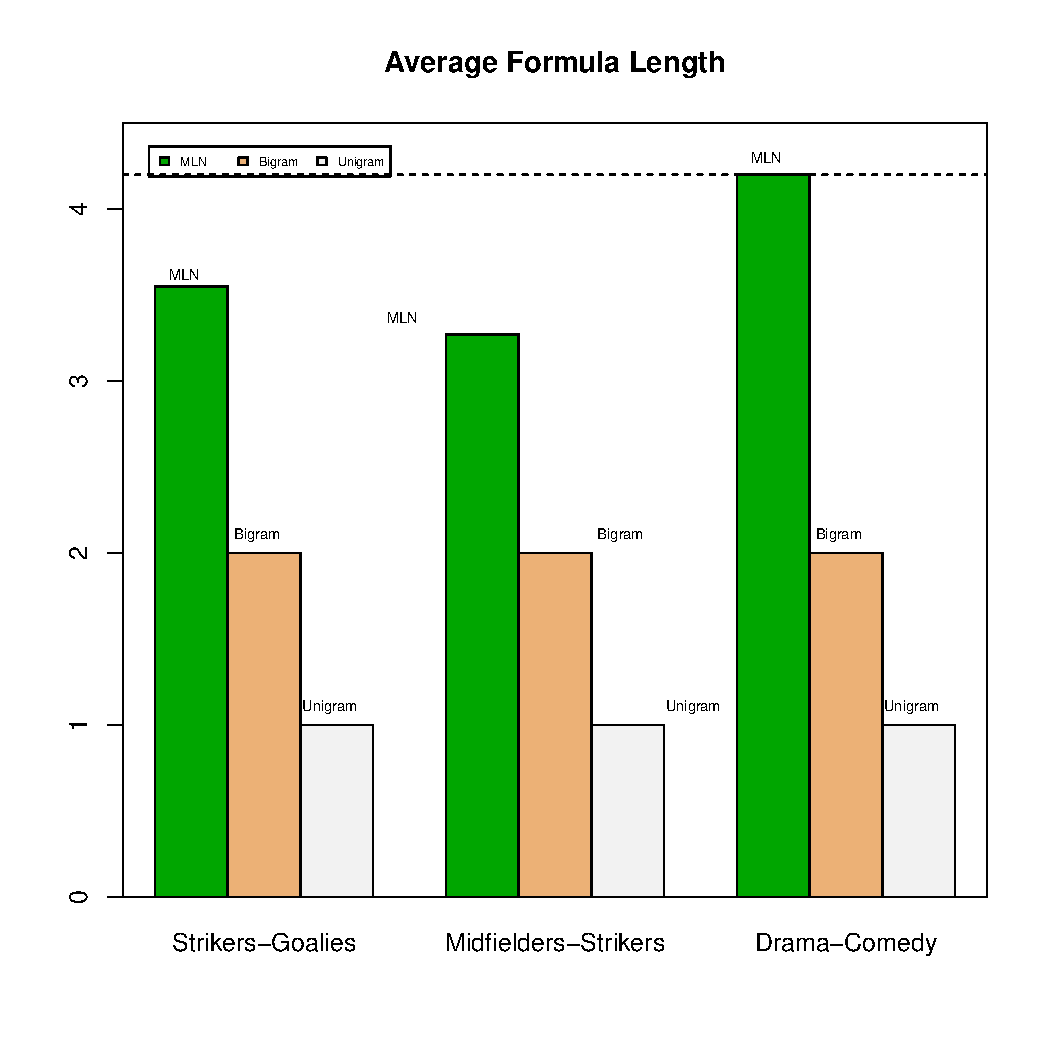
\includegraphics[width=0.48\textwidth]{Charts/formulaLength.pdf}}
							\subfigure[]{\label{fig:LowCor}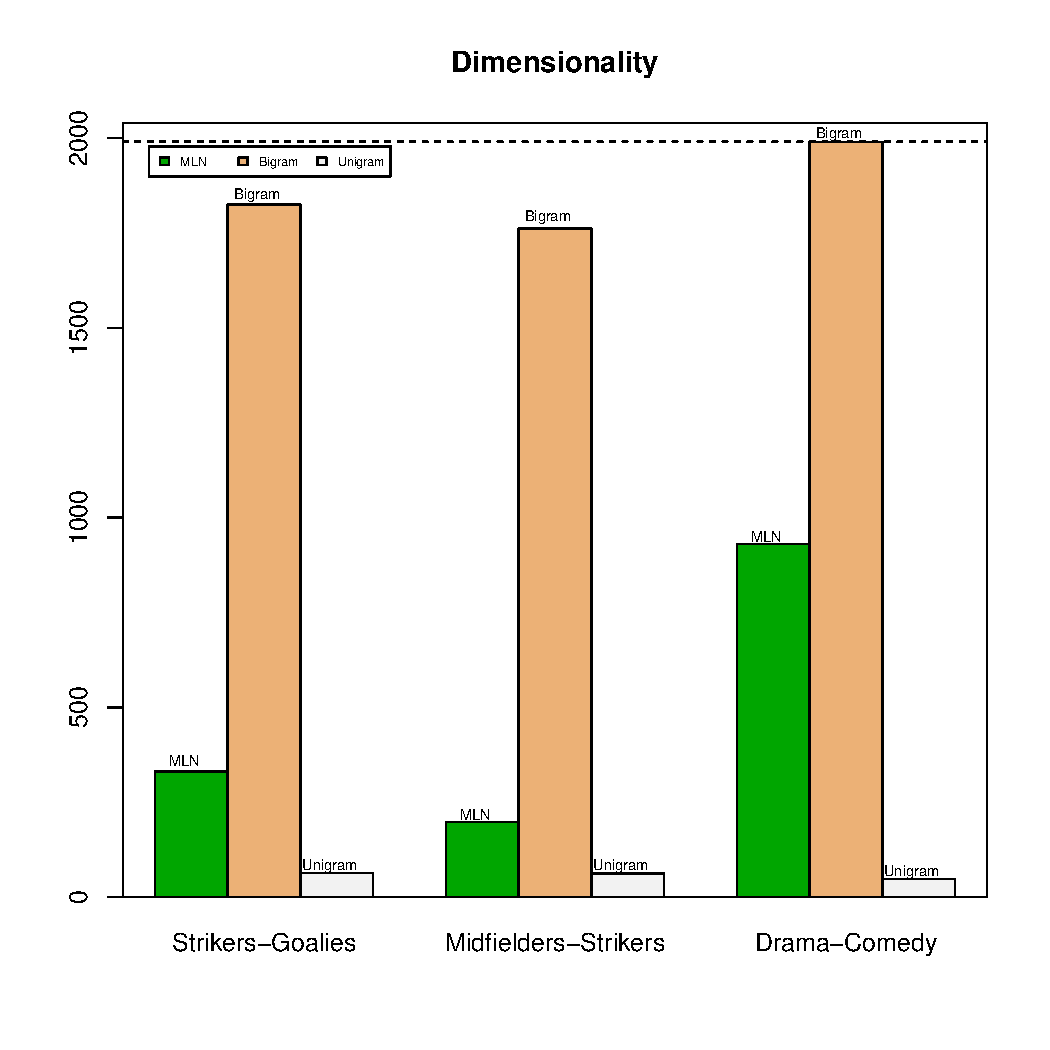
\includegraphics[width=0.5\textwidth]{Charts/dimensinality.pdf}}
							\subfigure[]{\label{fig:HighCor}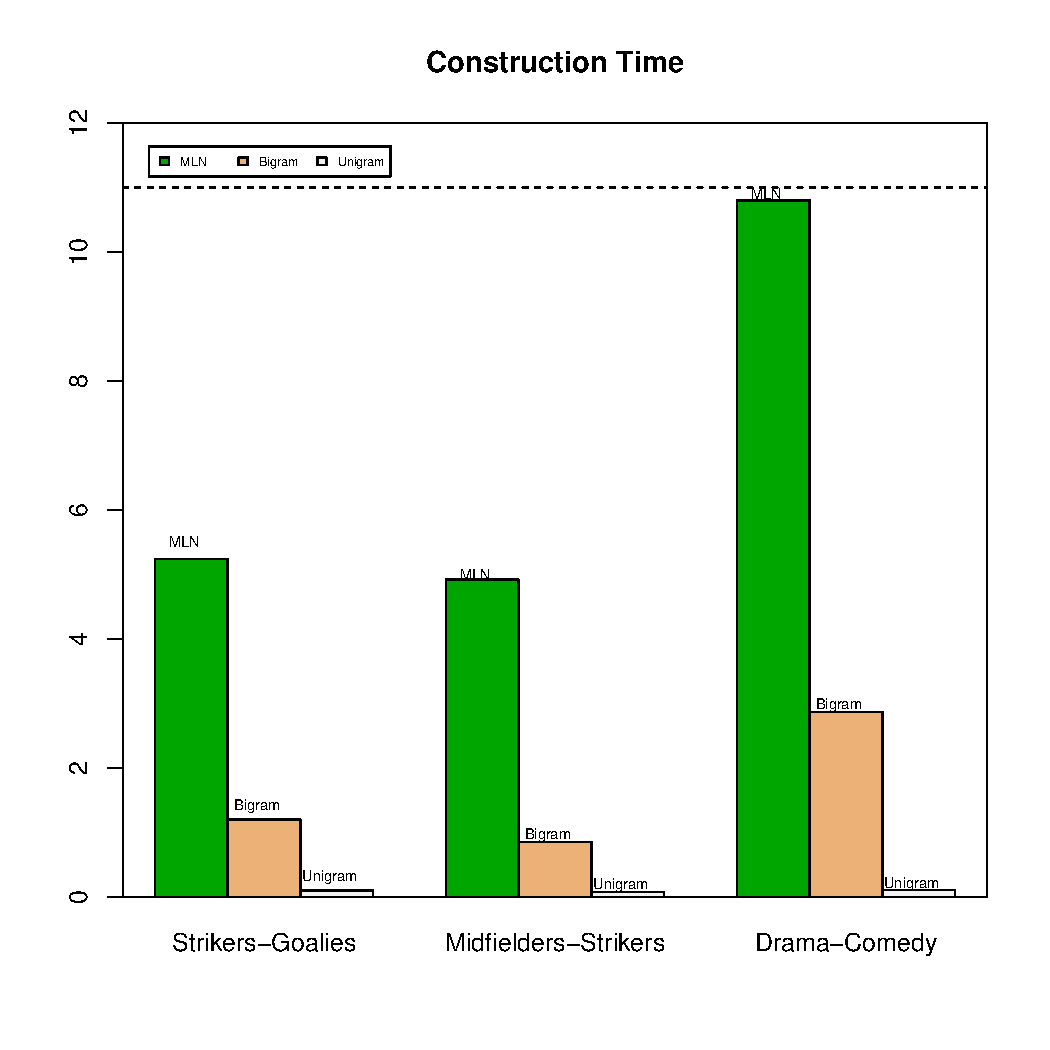
\includegraphics[width=0.5\textwidth]{Charts/ConstructionTime.pdf}}
							\caption{Comparison of complexity, dimensionality and construction time (min) for the attributes produced by different propositionalization methods}\label{fig:dimensionality}
						\end{figure}
		\subsection{Accuracy} 
		
		Figures~\ref{fig:propseSynth} and \ref{fig:propseReal} present detailed measurements of the AUC-ROC for different outlier propositionalization methods. There is no single propositionalization method that always leads to the best accuracy for all three outlier analysis methods. MLN propositionalization produces the best results on two datasets. It is always close to the maximum AUC score (never less than 0.1 AUC units away). Table~\ref{table:summary} summarizes the performance of the propositionalization methods for a fixed outlier detection algorithm. The $\mu(AUC)$ column reports the average AUC score over different datsets. A propositionalization method ``wins'' on a dataset if its AUC is at least 0.01 greater than that of others. A ``tie'' for first place earns 0.5 points. The total number of points is shown in the Wins columns. MLN-$\tf$ is revealed to be the best method in terms of average AUC, for all outlier detection methods. $\tf$ is, in a sense, the natural feature function for MLNs since the likelihood function of MLNs is defined in terms of formula grounding counts (equation 4.1). 		
		MLN-$\tf$ propositionalization scores the most wins when applied with $\lof$ or $\knn$ and a tie when applied with $\outrank$. Thus, methods that tend to treat attributes independently, such as $\lof$ and $\knn$, benefit from being provided complex attributes that summarize complex associations. Subspace analysis can utilize complex associations from bigram data, but requires much more time to do so than MLN propositionalization (see Table~\ref{table:outrank-time}).
		
		\begin{table*}
			
			\centering
			\caption{Summarizing the accuracy results of Figures~\ref{fig:propseReal} and~\ref{fig:propseSynth}: A propositionalization method is scored 1 point if it produces the best accuracy on a dataset, and 0.5 points if it ties. The table shows the total number of wins and average of AUC over all datasets.
				\label{table:summary}}
			\resizebox{0.9\textwidth}{!}{
				\begin{tabular}{|c|c|c|c|c|c|c|}
					\hline
					
					\begin{tabular}{p{4cm}}Propositionalization  $\rightarrow$\\ Outlier Detection Method $\downarrow$ \end{tabular}&\multicolumn{2}{|c|}{\begin{tabular}{p{1.5cm}}MLN-TF \end{tabular}}&\multicolumn{2}{|c|}{\begin{tabular}{p{2cm}}Bigram-IDF \end{tabular}}&\multicolumn{2}{|c|}{\begin{tabular}{p{2cm}}Unigram-TF \end{tabular}}\\\hline
					&Wins&$\mu(AUC)$&Wins&$\mu(AUC)$&Wins&$\mu(AUC)$\\\hline
					OutRank&\textbf{2.50}&\textbf{0.79}&\textbf{2.50}&0.70&1.00&0.64\\\hline
					KNN&\textbf{3.50}&\textbf{0.78}&1.50&0.67&1.50&0.67\\\hline
					LOF&\textbf{4.00}&\textbf{0.63}&1.00&0.55&1.00&0.61\\\hline
				\end{tabular}
				
			}
			
		\end{table*}
			%
			
			
									\begin{figure}
										\centering     %%% not \center
										\subfigure[ ]{\label{fig:Feature}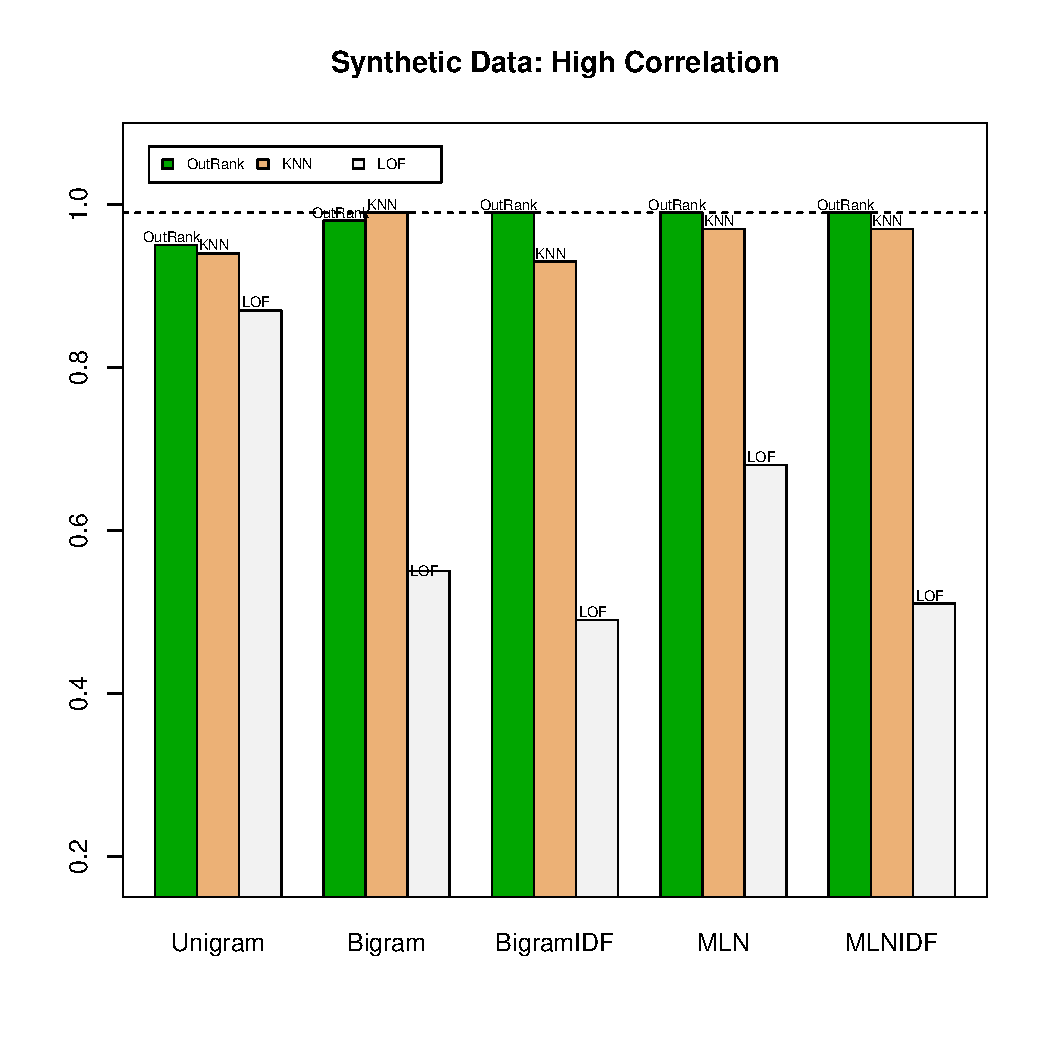
\includegraphics[width=0.48\textwidth]{Charts/highcorrelation-color.pdf}}
										\subfigure[]{\label{fig:LowCor}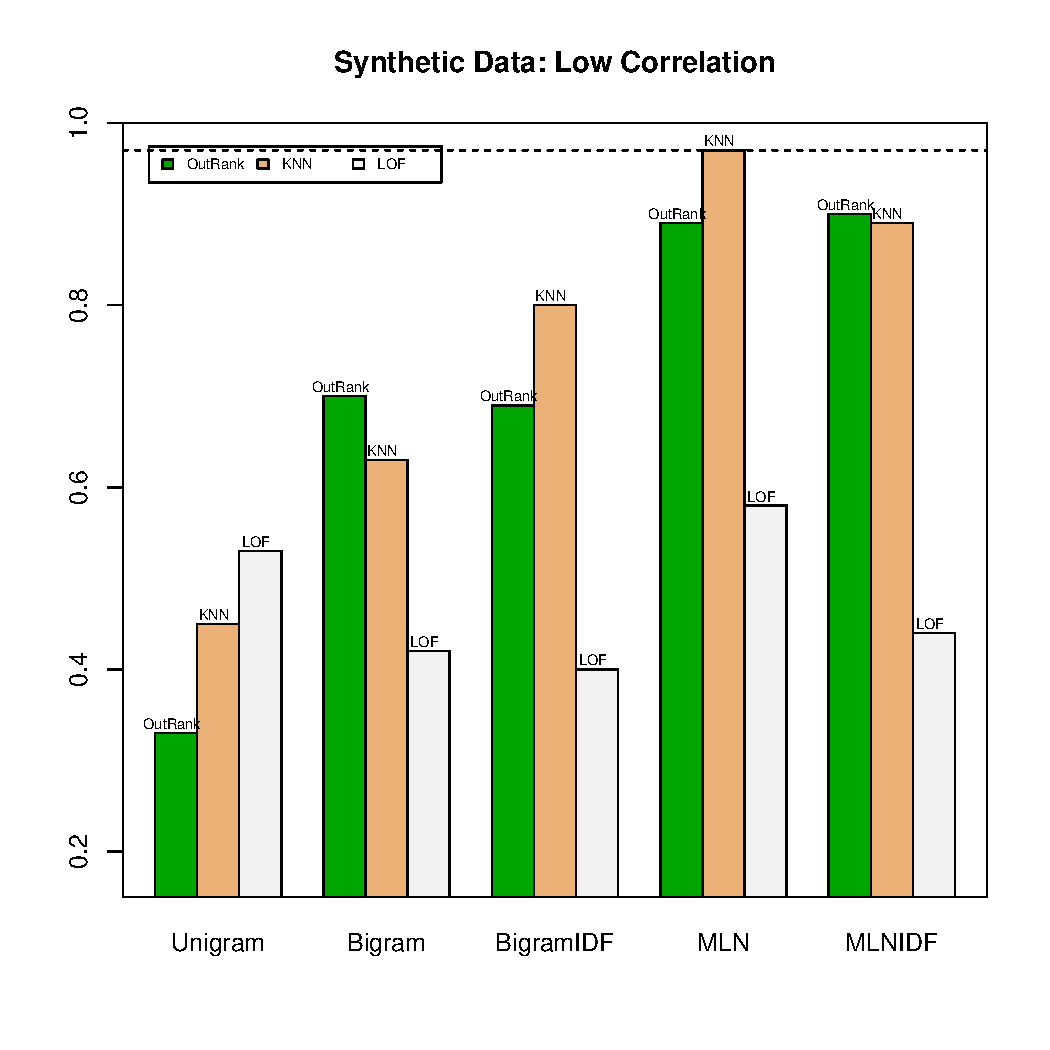
\includegraphics[width=0.5\textwidth]{Charts/lowcorrelation-color.pdf}}
										\subfigure[]{\label{fig:HighCor}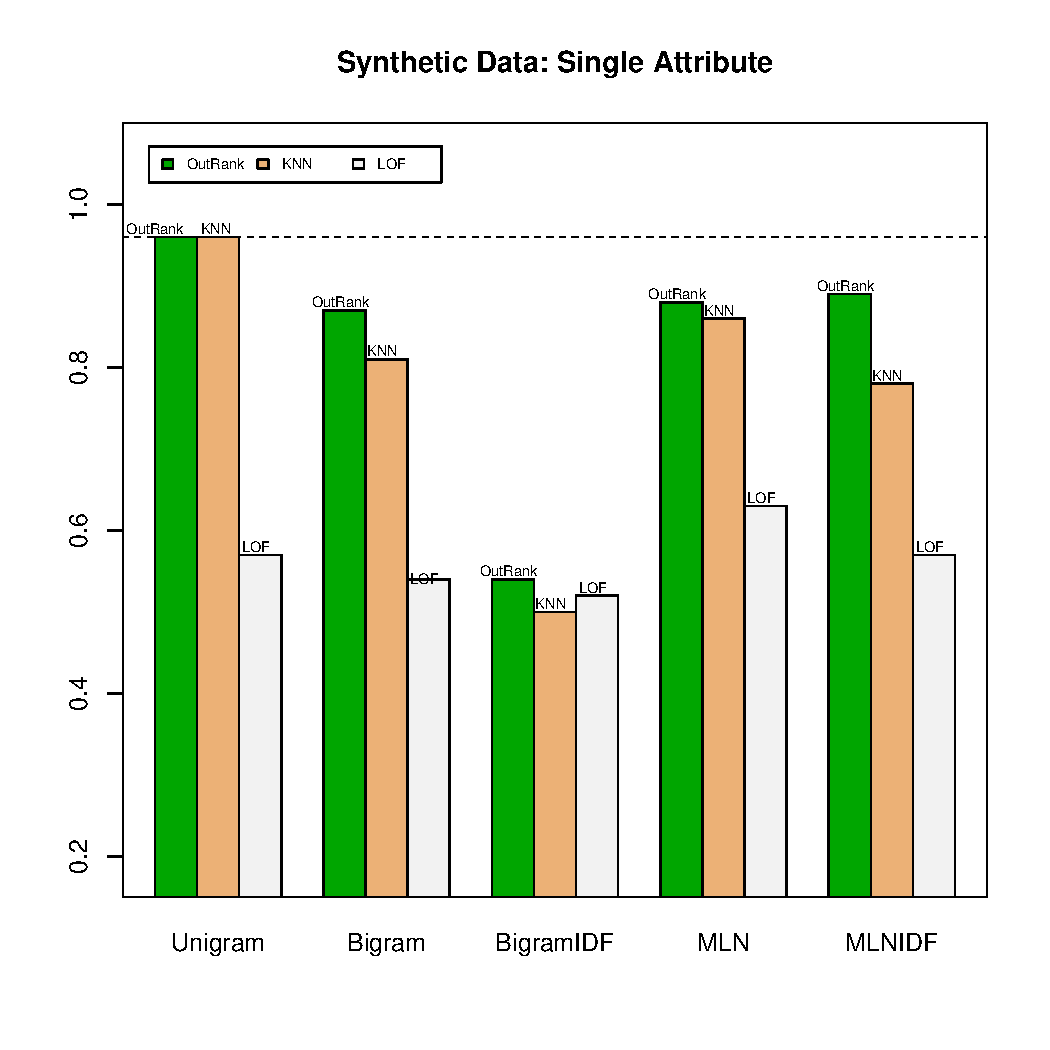
\includegraphics[width=0.5\textwidth]{Charts/SingleAttribute-color.pdf}}
										\caption{Accuracy for different Methods/Attribute Vector in the Synthetic datasets}\label{fig:propseSynth}
									\end{figure}
									
															\begin{figure}
																\centering     %%% not \center
																\subfigure[ ]{\label{fig:Feature}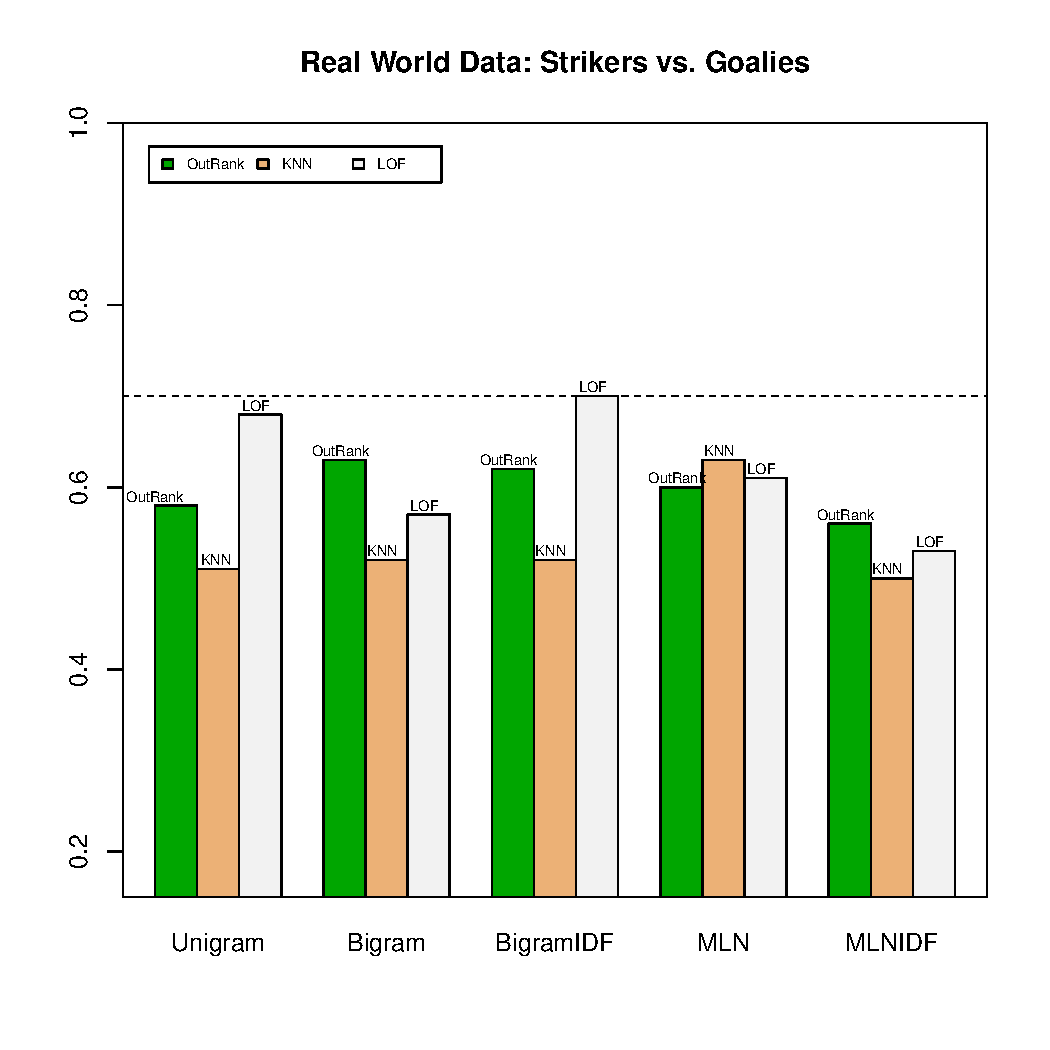
\includegraphics[width=0.48\textwidth]{Charts/strikersx.pdf}}
																\subfigure[]{\label{fig:LowCor}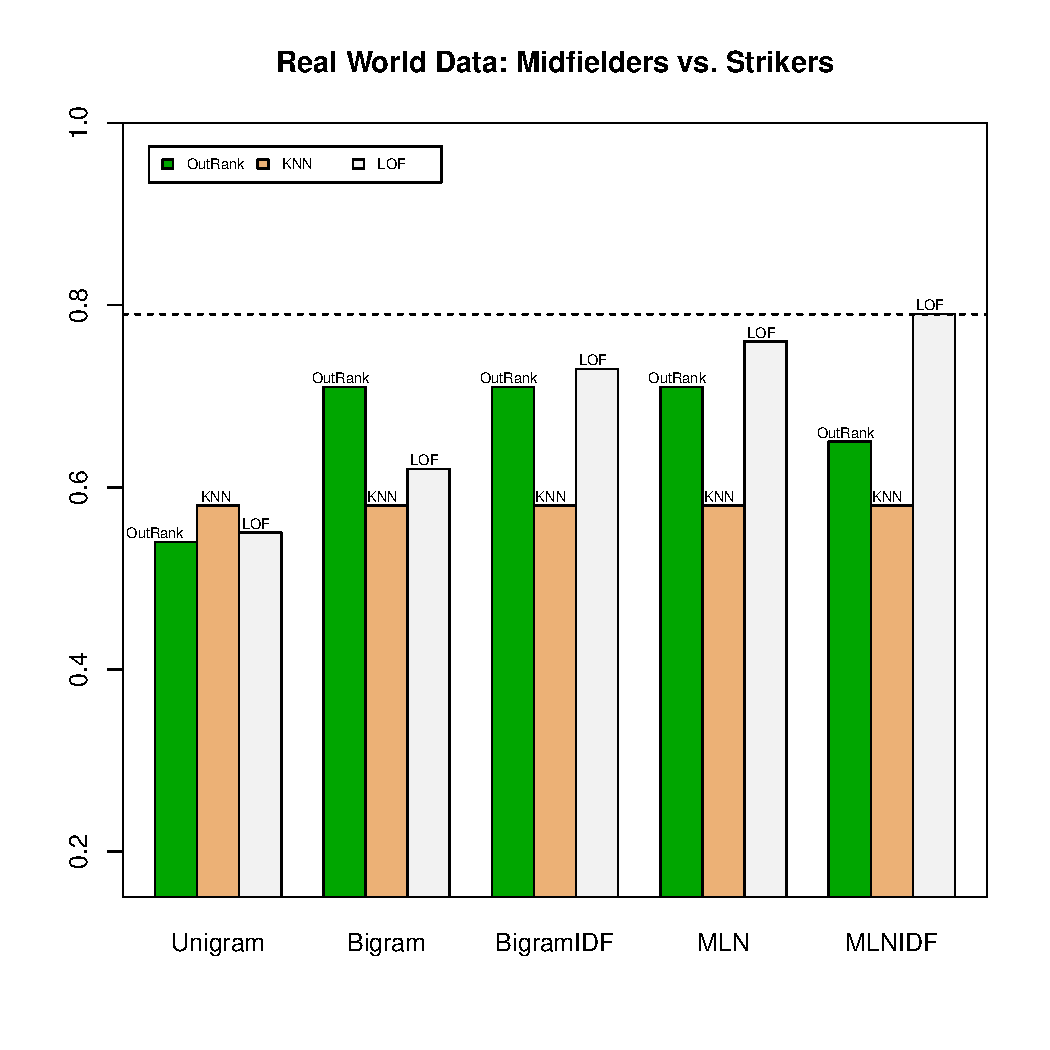
\includegraphics[width=0.5\textwidth]{Charts/midfielder-color.pdf}}
																\subfigure[]{\label{fig:HighCor}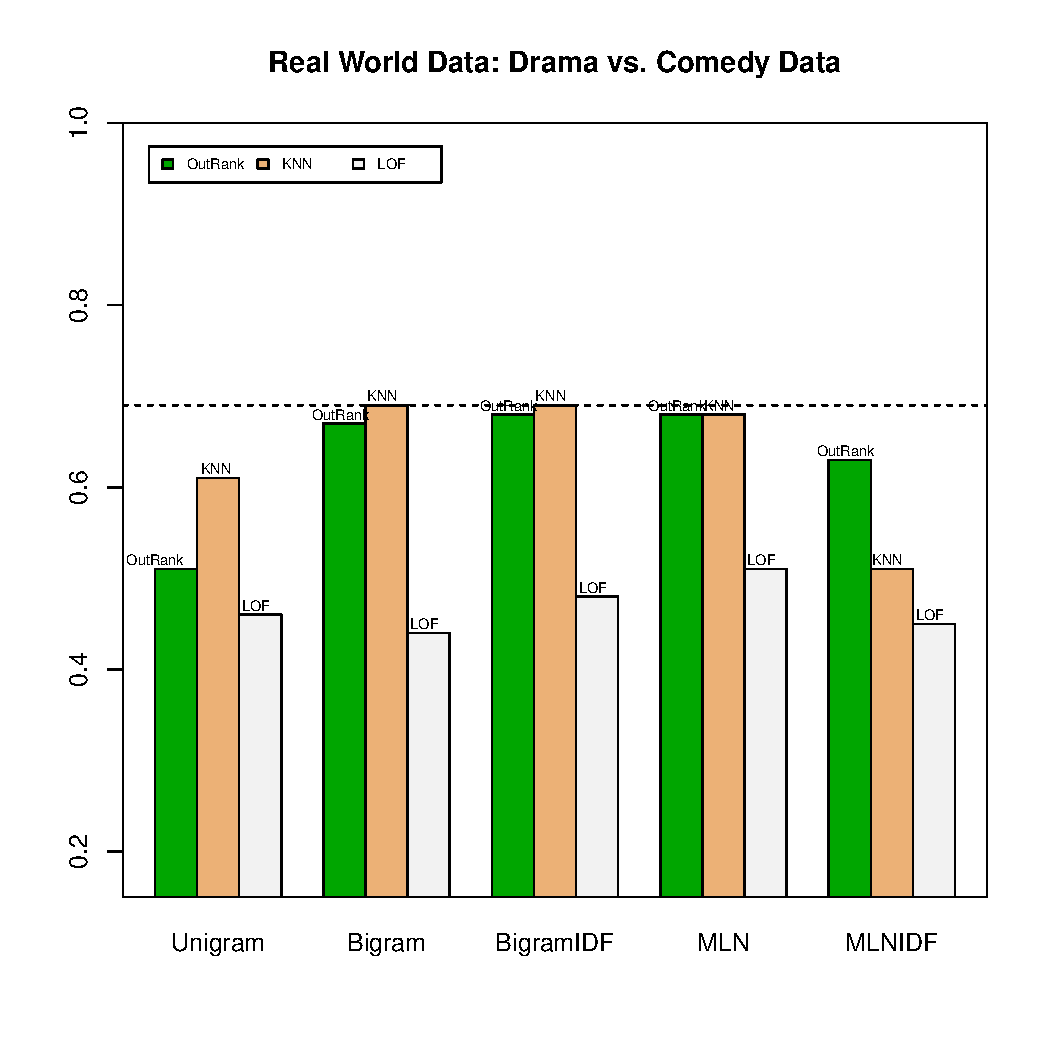
\includegraphics[width=0.5\textwidth]{Charts/imdb-color.pdf}}
																\caption{Accuracy for different Methods/Attribute Vector in the Real World datasets}\label{fig:propseReal}
															\end{figure}
									
								
			
			
			
			
%			
%											\begin{figure}
%												\centering
%												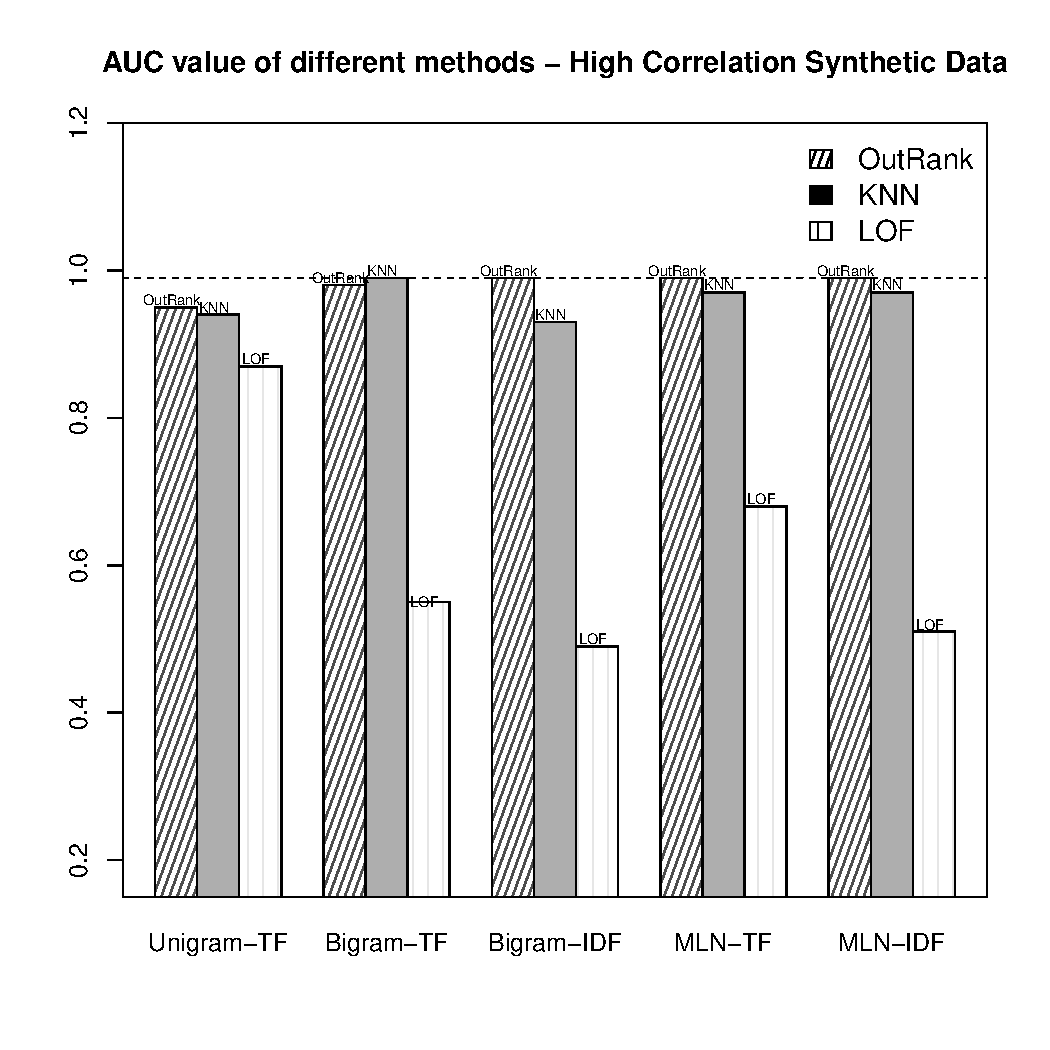
\includegraphics[width=0.6\textwidth] {Charts/highcorrelation.pdf}
%												\caption{System Flow
%													\label{main:b}}
%											\end{figure}
%											
%				
%						\end{figure}
%								\begin{figure}
%									\centering
%									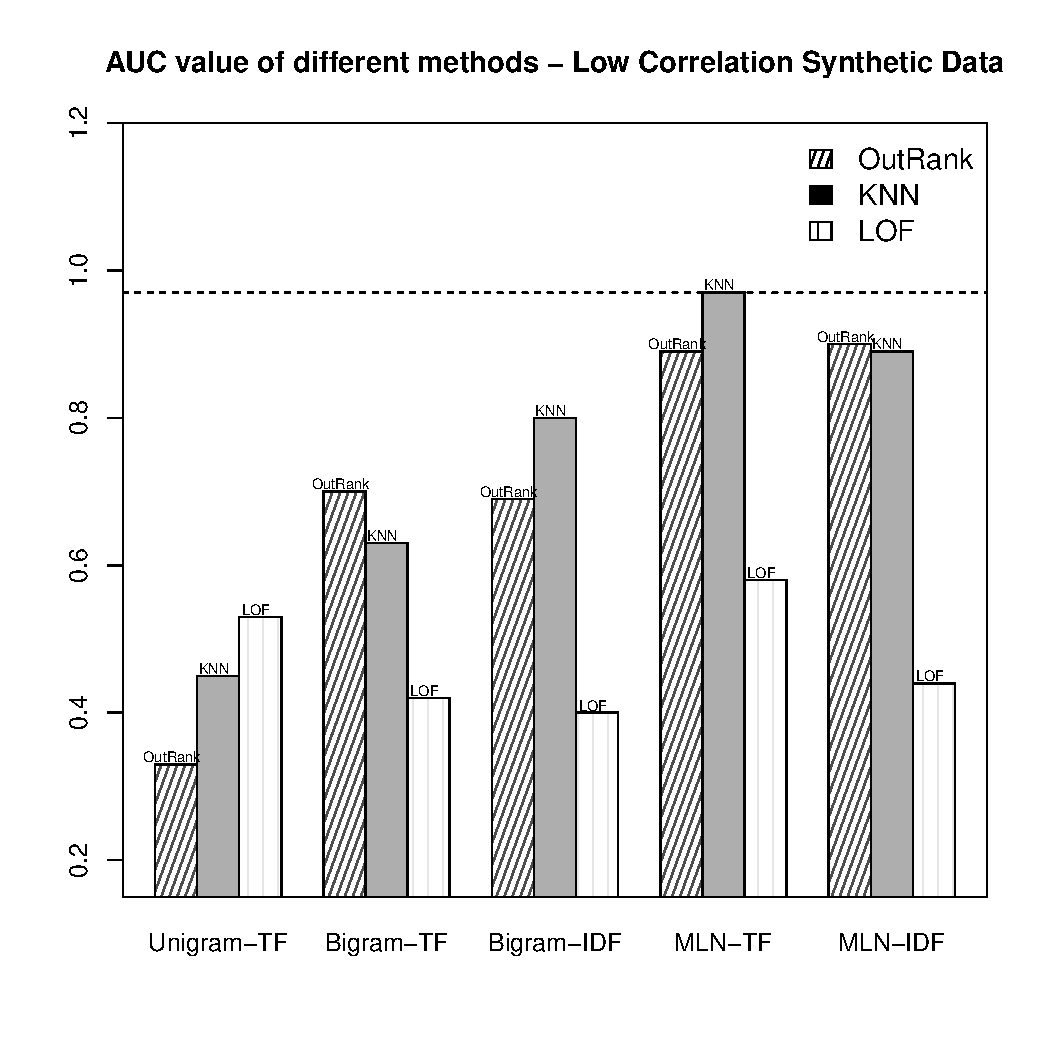
\includegraphics[width=0.6\textwidth] {Charts/lowcorrelation.pdf}
%									\caption{System Flow
%										\label{main:b}}
%								\end{figure}
%												
%												
%												
%					\begin{figure}
%						\centering
%						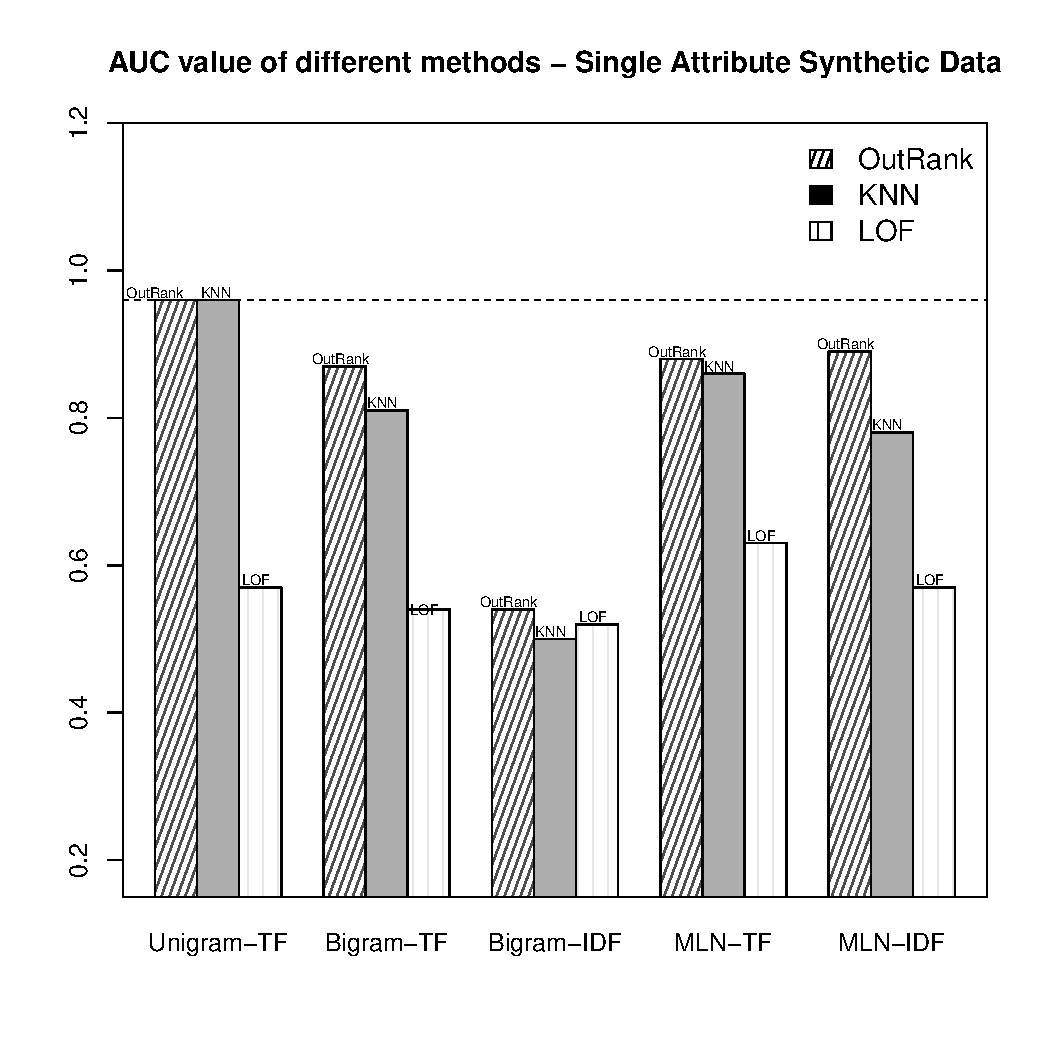
\includegraphics[width=0.6\textwidth] {Charts/SingleAttribute.pdf}
%						\caption{System Flow
%							\label{main:b}}
%					\end{figure}
					
					
			
			

			\section{Comparison With Propositionalization for Supervised Outlier Detection and Log-Likelihood} 
	
			In this section we compare our novel MLN propositionalization method
			with a previous propositionalization method that was developed for supervised classification problems. Since, to our knowledge, all previous propositionalization methods are for classification problems, in this section only we consider {\em supervised} outlier detection, where examples are labelled as ``normal'' and ``abnormal''. Given the ground truth labels, supervised outlier detection can be treated as a special case of classification \cite{Hodge2004}. Supervised outlier detection serves as a benchmark of the accuracy of unsupervised outlier detection: if the unsupervised method comes close to the accuracy of the supervised method, this indicates a good performance of the unsupervised method. 
			
			We report experiments with the state-of-the-art Treeliker propositionalization method \cite{kuzelka2008}. We used the implementation of Treeliker available in the ClowdFlows platform \cite{Kranjc2012}, which supports the MySQL data format. The HiFi algorithm from \cite{kuzelka2008} has been used with minimum frequency specified as 0.2, maximum size of features to be 10 and sample size as 5. We train and test Treeliker on the same dataset with ground truth labels as classification target. So the way we use Treeliker gives it two advantages over MLN propositionalization: It sees the ground truth labels, and it is tested on the training data. On almost all real-world datasets, this translates into a higher AUC score, except for the Striker-Midfielder problem using $\lof$ (0.61 for MLN vs. 0.56 for Treeliker). MLN propositionalization comes close to the Treeliker score, the only substantial difference occurs with $\lof$ on the Striker-Goalie problem (0.76 for MLN vs. 0.84 for Treeliker).  On the synthetic data, the MLN method performs even better, beating the Treeliker propositionalization by a substantial margin. Given the advantages for the supervised setting, this is a very good performance for MLN propositionalization. We emphasize that this is not a criticism of Treeliker as a propositionalization method, because it is not designed for outlier detection problems. Rather, our conclusion is that new methods provide value for the problem of propositionalization for outlier detection. 
			
			\begin{table*}
				
				\centering
				\resizebox{0.6\textwidth}{!}{
					\begin{tabular}{llcccc}
						\hline
						
						Database&\begin{tabular} {p{1.5cm}}Outlier Method\end{tabular}&\begin{tabular} {p{1.5cm}} Treeliker \\ AUC value \end{tabular}& \begin{tabular} {p{1.5cm}} MLN-TF \\ AUC value \end{tabular}&\begin{tabular}{p{1.5 cm}}%\\\hline
						%	Treeliker\\VectorSize
					%	\end{tabular}&\begin{tabular}{p{1.5 cm}}
					%	MLN-TF\\VectorSize
					\end{tabular}\\\hline
				%	Single Attribute&OutRank& NA&\textbf{0.88}&303&6\\\hline
					Single Attribute&KNN& 0.65&\textbf{0.86}\\\hline%&303&6\\\hline
					Single Attribute&LOF& 0.53&\textbf{0.63}\\\hline%&303&6	
				%	High Correlation&OutRank& NA&\textbf{0.99}&302&6\\\hline
					High Correlation&KNN& 0.66&\textbf{0.97}\\\hline%&302&6\\\hline
					High Correlation&LOF& 0.57&\textbf{0.68}\\\hline%&302&6	\\\hline
			%		Low Correlation&OutRank& NA&\textbf{0.89}&302&6\\\hline
					Low Correlation&KNN& 0.65&\textbf{0.97}\\\hline%&302&6\\\hline
					Low Correlation&LOF& 0.56&\textbf{0.58}\\\hline%&302&6	\\\hline
					
			%		Striker Goalie&OutRank& NA&\textbf{0.71}&3,620&331\\\hline
					Striker Goalie &KNN& \textbf{0.6}&0.58\\\hline%&3,620&331\\\hline
					Striker Goalie &LOF& \textbf{0.84}&0.76\\\hline%&3,620&331	\\\hline
			%		Midfielder Striker&OutRank& NA&\textbf{0.6}&5,093&198\\\hline
					Midfielder Striker&KNN& \textbf{0.65}&0.63\\\hline%&5,093&198\\\hline
					Midfielder Striker&LOF&0.56&\textbf{0.61}\\\hline%&5,093&198	\\\hline
					
				\end{tabular}
				
			}
			\caption{Accuracy of Treeliker for different databases and outlier techniques. Bold values represent the cases where Treeliker outperforms other methods. 
				\label{table:Treeliker}}
		\end{table*}
%		\subsection{Result of Log-likelihood}
%		The log-likelihood method \cite{FatemehRiahi2013a} combines learned MLN weights with MLN structure. The outlier score is the weighted sum of formula groundings for each potential outlier individual. The accuracy of the log-likelihood method is similar to that of Markov Logic propositionalization, depending on the outlier analysis method (e.g., for $\outrank$ and $\knn$ the average AUC difference is 0.01 in favor of log-likelihood, for $\lof$ log-likelihood does much better; the average of AUC difference is 0.17).
%		Table~\ref{table:Metric Comparison} shows the performance of Log-likelihood in different datasets.
%		\begin{table}[!htbp]
%			
%			
%			\centering
%			\resizebox{0.5\textwidth}{!}{
%				\begin{tabular}{|l|l|}
%					\hline
%					Dataset & \loglikelihood\\ \hline
%					
%					Synthetic Data-High Correlation &0.98 \\ \hline
%					Synthetic Data-Low Correlation &0.95 \\ \hline
%					Synthetic Data-Single Feature&0.98 \\ \hline
%					Real Data-Strikers vs. Goalies& 0.65\\ \hline
%					Real Data-Midfielders vs. Strikers&0.64 \\ \hline
%					Real Data-Drama vs. Comedy&0.63 \\ \hline
%				\end{tabular}}
%				\caption{$\auc$ of Log-likelihood in different datasets. 
%					%For relationships please see text.
%					\label{table:Metric Comparison}}
%			\end{table}
	\section{Conclusion}		
	In this chapter we developed a pipeline propositionalization approach where the information from multiple data tables is summarized in a single data table. The key step is to find a set of relevant logical formulas that define conjunctive attributes of potential outlier individuals as sum. We utilized Markov Logic Network learning for this task. In an empirical comparison with the baseline wordification approach of enumerating all conjunctive formulas up to length 2, Markov Logic propositionalization showed several advantages: 1) The set of formulas learned was substantially smaller, leading to smaller data tables and faster outlier detection. 2) The formulas learned were longer, representing more complex relational patterns. 3) For a fixed single-table outlier analysis method, the average detection accuracy was higher.
	
	We view this work as an initial step in the topic of propositionalization for outlier detection, there are several fruitful directions for future work. While Markov Logic networks are a prominent generative model class for relational data, our approach can be used with  other generative models; this opens a new application area for statistical-relational learning. Dimensionality reduction techniques can be employed after propositionalization to reduce the size of the data tables before outlier detection methods are used. Propositionalization algorithms that were developed for classification could be adapted for unsupervised outlier detection by using a feature selection score that is relevant for outlier detection, rather than supervised classification.
	
	Another direction for future work is to leverage graph-based descriptive features in our generative model learning process.
	These features proved to be efficient in discovering patterns for anomaly detection task in ODDBALL~\cite{Akoglu2010}. Examples of such features in our datasets include: number of matches a player has played, number of reviews a movie has received, and features related to the extent of interaction between players.


\chapter{Metric-based Outlier Detection}
\label{chap:five}

In chapter~\ref{chap:four} we introduced a pipeline propositionalization method to convert object-relational data to a single data table. By summarizing the information from relational data in one data table, we showed that we can leverage the many previous outlier detection methods that were designed for single data table. The goal of this chapter is to introduce an unsupervised 
statistical outlier detection method  to the case of object-relational data without converting the data
to i.i.d. propositional format.
%This chapter extends unsupervised 
%statistical  outlier detection to the case of object-relational data. Object-relational data represent a complex heterogeneous network~\cite{Gao2010}, which comprises objects of different types, links among these objects, also of different types, and attributes of these links. 
For each object there is a probability distribution over the features of related objects. For example, for each soccer team there is a distribution over the features of its players.
%In relational structures, an individual object may display a complex pattern of probabilistic associations among its attributes, the attributes of linked objects, and the attributes of its links. These relationships represent a complex heterogeneous network of objects. 
This special structure prohibits a direct vectorial data representation. We apply state-of-the-art probabilistic modelling techniques for object-relational data that construct a graphical model (Bayesian network), which compactly represents probabilistic associations in the data. We propose a new  metric, based on the learned object-relational model, that quantifies the extent to which the individual association pattern of a potential outlier deviates from that of the whole population. The metric is based on {\em the likelihood ratio} of two parameter vectors: One that represents the population associations, and another that represents the individual associations. 
The likelihood ratio can be improved for outlier detection by applying two transformations: (1) a mutual information decomposition and (2) replacing log-likelihood differences by log-likelihood distances. 
Our method is validated on synthetic datasets and on real-world data sets about soccer matches and movies. Compared to baseline methods, our novel transformed likelihood ratio achieved the best detection accuracy 
%(AUC) 
%true positive/negative rates 
on all datasets. 
\section{Introduction} 
Outlier detection is an important data analysis task in many domains. Statistical approaches to unsupervised outlier detection are based on a generative model of the data~\cite{aggarwal2013}. The generative model represents normal behavior. An individual object is deemed an outlier if  the model assigns sufficiently low likelihood to generating it. 
We propose a new method for extending statistical  outlier detection to the case of object-relational data using a novel likelihood-ratio comparison for probabilistic models. 

%The object-relational data model has been introduced in Chapter\ref{chap:three}
\paragraph{Approach} 
Figure~\ref{fig:flow} illustrates these concepts and the system flow for computing an outlier score. A class-model Bayesian network (BN) structure is learned with data for the entire population. The nodes in the BN represent attributes for links, of multiple types, and attributes of objects, also of multiple types. To learn the BN model, we apply techniques from statistical-relational learning, a  recent field that combines AI and machine learning \cite{SRL2007,Schulte2012,Domingos2009}. 
%The BN provides dimensionality reduction, in the sense that it leverages independencies to represent the data distribution with exponentially fewer parameters than a non-factorized parametrization. 
Given a set of parameter values and an input database, it is possible to compute a {\em class model likelihood} that quantifies how well the BN fits the object data. The class model likelihood uses BN parameter values {\em estimated from the entire class data.} This  is a relational extension of the standard log-likelihood method for i.i.d. vectorial data, which uses the likelihood of a data point as its outlier score. %This can be adapted for object-relational data as follows.
%The Bayes net structure represents the normal pattern of associations among links and attributes  by the well-known d-separation criterion: Two nodes are probabilistically independent if they are d-separated. 

While the class model likelihood is a good baseline score, it can be improved by comparing it to {\em the object model likelihood}, which uses BN parameter values {\em estimated from the object data.}
The {\em model log-likelihood ratio} (LR) is the log-ratio of the object model likelihood to the class model likelihood. This ratio quantifies how the probabilistic associations that hold in the general population deviate from the associations in the object data substructure.
While the 
likelihood ratio discriminates relational outliers better than the class model likelihood alone, it can be improved further by applying two transformations: (1) a mutual information decomposition, and (2) replacing log-likelihood differences by log-likelihood distances. We refer to the resulting novel score as the {\em log-likelihood distance}.
	\begin{figure}
		\centering
		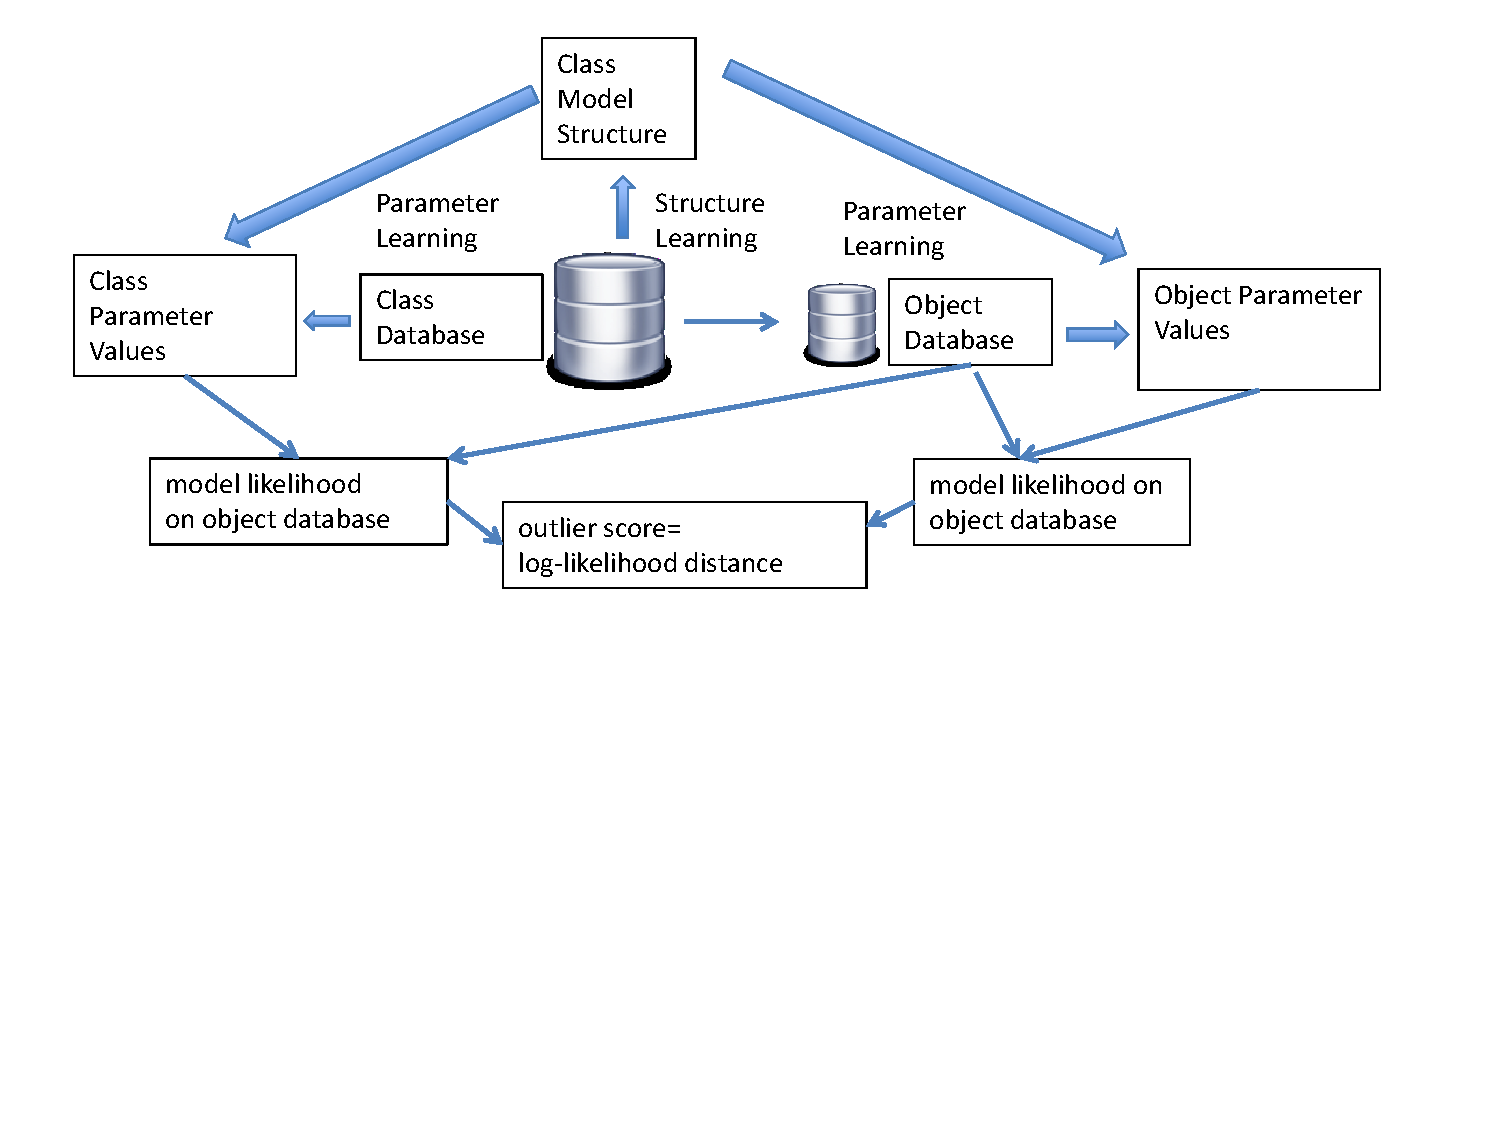
\includegraphics[width=1\textwidth]{figures/sysFlow.pdf}
		
		\caption{Computation of outlier score. 
			\label{fig:flow}}
	\end{figure}
%
%This paper considers outlier detection for object-oriented data. Object-orientation is one of the main data models for representing structured data~\cite{Ramakrishnan2003,Koller1997}. It is a natural data model for the widely used XML format, where nodes in the XML document tree are viewed as objects.\footnote{\url{http://www.w3.org/DOM/}} 
%%
%%The object-oriented data model was inspired by object-oriented programming. 
%%There are different formulations of the object-oriented data model
%%; the concepts in this paper apply to data objects in general. 
%The main 
%characteristics of data objects that we utilize in this paper are the following. (1) {\em Object Identity.} Each object has a unique identifier that is the same across contexts. For example, a player has a name that identifies him in different matches. (2) {\em Class Membership.} An object is an instance of a class, which is a collection of similar objects. In particular, objects in the same class share a set of attributes. For example, van Persie is a player object that belongs to the class striker, which is a subclass of the  class player. (3) {\em Component Relationships.} Atomic objects have attributes but no components. Complex objects contain other objects as components or parts. For example, a match involves two teams, and each team comprises a set of players for that match. 
%
%%Standard outlier or anomaly detection methods are defined for a data model of atomic objects from the same class without subobjects. 
%%``flat'' feature vectors, which are atomic objects with no subobjects. 
%The class and component hierarchies represent information about objects that an outlier detection method should take into account. We achieve this in two steps. Step 1: the component hierarchy is used to compute an {\em object profile}. The object profile is a data structure that specifies the object's attributes and the attributes of related objects. Two objects are related if there is a chain of components connecting them. For example, for each soccer player, there is a player distribution over: the player's attributes, the player's team's results in matches, and the actions of the player in matches.
%%For example, for each soccer team, there is a team distribution over: the team's attributes, the team's results in matches, and the actions of the team's players in matches. 
%Step 2: Given a set of object profiles, compute an outlier score that measures how the object's profile differs from the profiles of other objects in its class. We develop a probabilistic approach where:
%
%\begin{quote}
%	Object Outlier Score = Score between object distribution and class distribution
%\end{quote}
%
%For each object, the object distribution is a joint distribution over the object's attributes and the attributes of related objects. The object distribution can be computed from counts in the object profile. The class distribution is the distribution of a randomly chosen object in the class. 
%
%
%%
%This approach allows us to apply ideas from the well-researched topic of probability divergences to the problem of object outlier detection. A baseline divergence concept is the standard Kullback-Leibler divergence (KLD). KLD computes the expected log-{\em difference} between two joint distributions. Our argument in this paper is that for outlier detection, we ought to use instead the expected log-{\em distance} between two joint distributions. The reason is that averaging distribution differences loses information when two distribution differences point in opposite directions, and cancel each other out. We refer to our novel divergence as the expected log-distance divergence (ELD).
%%\vspace{-5mm}
\paragraph{Evaluation} Our code and datasets are available on-line at \cite{url}.
Our performance evaluation follows the design of previous outlier detection studies~\cite{Gao2010,aggarwal2013},
%~\cite{Cansado2008, Muller2012},
%\footnote{review} 
where the methods are scored against a test set of known outliers.  
%and case studies assess their output on specific cases. 
%
We use three synthetic and two real-world datasets, from the UK Premier Soccer League and the Internet Movie Database (IMDb). On the synthetic data we have known ground truth. For the real-world data, we use a anomaly injection method discussed in chapter~\ref{chap:two}, where one object class is designated as normal and objects from outside the class are the outliers. For example, we compare goalies as outliers against the class of strikers as normal objects. 
%Given ground truth, an outlier detection method can be scored in terms of true positives and negatives, summarized using AUC~\cite{Muller2012}.\footnote{review} 
%Comparisons outlier scores include the class model likelihood, our novel log-likelihood distance, and likelihood-based scores intermediate to these two. 
%Previous outlier analysis for similar structured data  \cite{Breunig2000} used a preprocessing step where the structured data are converted to vectorial data that represent atomic objects. This conversion is usually done by aggregation, which tends to lose information.
%, for instance using counts as attributes in an attribute vector. After aggregation, we evaluate 
%After aggregation, standard outlier detection methods for independent data points can be applied; we use three as baseline methods for our evaluation ($\outrank$, $\lof$, and $\knn$).
On all datasets the log-likelihood distance metric achieves the best detection accuracy compared to baseline methods. 

We also offer case studies where we assess whether individuals that our score ranks as highly unusual in their class are, indeed, unusual. 
%This assessment looks at the object profile data of these individuals. 
The case studies illustrate that our outlier score is {\em easy to interpret}, because the Bayesian network provides a sum decomposition of the data distributions by features. Interpretability is very important for users of an outlier detection method as there is often no ground truth to 
evaluate outliers suggested by the method. %With regards to the cost of computing the divergence outlier score, we show that a Bayesian network representation of the object distributions can speed up the computation by orders of magnitude.

%One of our baseline methods is a variant of the distribution divergence approach that we introduce in this paper, where Kullback-Leibler convergence is the used as the outlier score. 
%
%we rank both normal and outlier individuals against the distribution of the normal class only. For example, we 
%compare the attribute distributions of both goalies and strikers against the class distribution of strikers. 
%
%We compare the detection accuracy of our novel mutual information divergence with the Kullback-Leibler convergence.
%basing a distribution divergence on the expected distance to basing it on the expected difference. 
%As regards to previous methods, to our knowledge ours is the first outlier detection method tailored for object-oriented data. Previous outlier analysis for structured data similar to ours (e.g., sports data) \cite{Breunig2000} used a preprocessing step where the structured data are converted to a matrix of attribute vectors that represent atomic objects. 
%  outlier detection methods for the atomic objects data model---based  on a single data matrix---have been applied to datasets similar to those that we examine  
% previously analyzed with 
%Standard outlier detection methods require as input a data matrix, that represents attributes of atomic objects from the same class. It is therefore not possible to provide structured data as input directly to such methods. In previous outlier detection work, data matrix methods were applied by 
%Converting object-oriented data to a data matrix can be done by aggregation.
%, for instance using counts as attributes in an attribute vector. After aggregation, we evaluate 
%After aggregation, standard outlier detection methods for independent data points can be applied; we use three as baseline methods for our evaluation ($\outrank$, $\lof$, and $\knn$).
% three aggregation approaches  using a subspace outlier ranking method, $\outrank$, a density-based outlier detection method, the Local Outlier Factor ($\lof$), and a distance based outlier detection method, $\knn$.  On all datasets, the log-distance divergence achieves the best detection accuracy.
%We also offer case studies where we discuss why highly ranked individuals are indeed unusual in their class. The case studies illustrate that our divergence outlier score is easy to interpret, because it is based on a sum decomposition of the joint distributions. Interpretability is very important for users of an outlier detection method as there is often no ground truth to 
%evaluate outliers indicated by the method. 
%\vspace{-5mm}
\paragraph{Contributions} Our main contributions in this chapter may be 
summarized as follows.

\begin{enumerate} 
	\item The first approach to outlier detection for structured data that is based on a probabilistic model. 
	\item A new model-based outlier score based on a novel model likelihood comparison, the log-likelihood distance. 
\end{enumerate}
% \vspace{-0.5cm}

	\section{Related Work}
%	Outlier detection is a densely researched field, for surveys please see~\cite{aggarwal2013, Akoglu2015}.
	In chapter~\ref{chap:two} we reviewed some outlier detection methods designed for the structured data. Our method falls in the category of {\em unsupervised} statistical model-based approaches. To our knowledge, ours is the first model-based method tailored for object-relational data.
	Figure~\ref{fig:novelty} provides a tree picture of where our method is situated with respect to other outlier detection methods and other data models. In the following we review a generative model-based method that has been used as a baseline to our work.
	%For an outlier detection survey please see~\cite{aggarwal2013}.
	%\cite{Hodge2004,aggarwal2013}. 
%	Our method falls in the category of {\em unsupervised} statistical model-based approaches. To our knowledge, ours is the first model-based method tailored for object-relational data.% Like other model-based approaches, it detects {\em global outliers.} Aggarwal \cite{aggarwal2013} defines a global outlier to be a data point that notably deviates from the rest of the population. We review relevant approaches from different data models, the most common atomic object model---where data is represented by vectors---and structured data models.\\

%	\textit{a) Attribute Vector Data Model:}
%
%	By far most work on outlier detection considers atomic objects with flat feature vectors.
%	%, or nonhierarchical structures like time series. 
%	This leads to an impedance mismatch: 
%	The required input format for these outlier detection methods is a single data matrix, not a structured dataset. For example, one cannot provide a relational database as input. This mismatch is not simply a question of choosing a file format, but instead reflects a different underlying data model: complex objects with both attributes and component objects vs. atomic objects with attributes only. 
%	%
%	It is possible to ``flatten'' structured data by converting it to unstructured feature vectors, for instance by using aggregate functions. 
%	Flattening incurs some loss of information but allows us to apply the many feature vector methods.
%	%\cite{Elke2013}. 
%	We evaluated the aggregation approach in this paper by applying three standard methods for outlier detection.
%	%for three major approaches to outlier detection: distance-based, density-based, and subspace clustering. 
%	%
%	%Subspace clustering methods (e.g., \cite{Muller2012,Kriegel2009}) are similar to our work in the sense that they aim to decompose a complex data space. They find complex deviations that are noticeable only in a data subspace. A common approach is to discover datapoints that show unexpected deviations in similar subspaces. Our approach instead develops a joint measure of how dissimilar the target object profile distribution is to the class distribution over the entire data space. Given that object and class distributions are represented by an object-oriented Bayesian network \cite{Koller1997}, the network structure defines subspaces. The joint divergence measure {\em mathematically decomposes} into subspace measures that quantify how dissimilar the target object profile distribution is in the subspaces defined by the network, compared to the class distribution in the same subspace.
%	
%	Work on atomic contextual  outliers \cite{Tang2013} is like ours in that it considers the distinctness of a target individual from a reference class. A reference class is not specified for each object,
%	%as a property of the object, 
%	but is constructed as part of outlier detection. 
%	Our work could be combined with a class discovery approach by providing a score of how informative the inferred classes are. 
	\begin{figure}
		\centering
		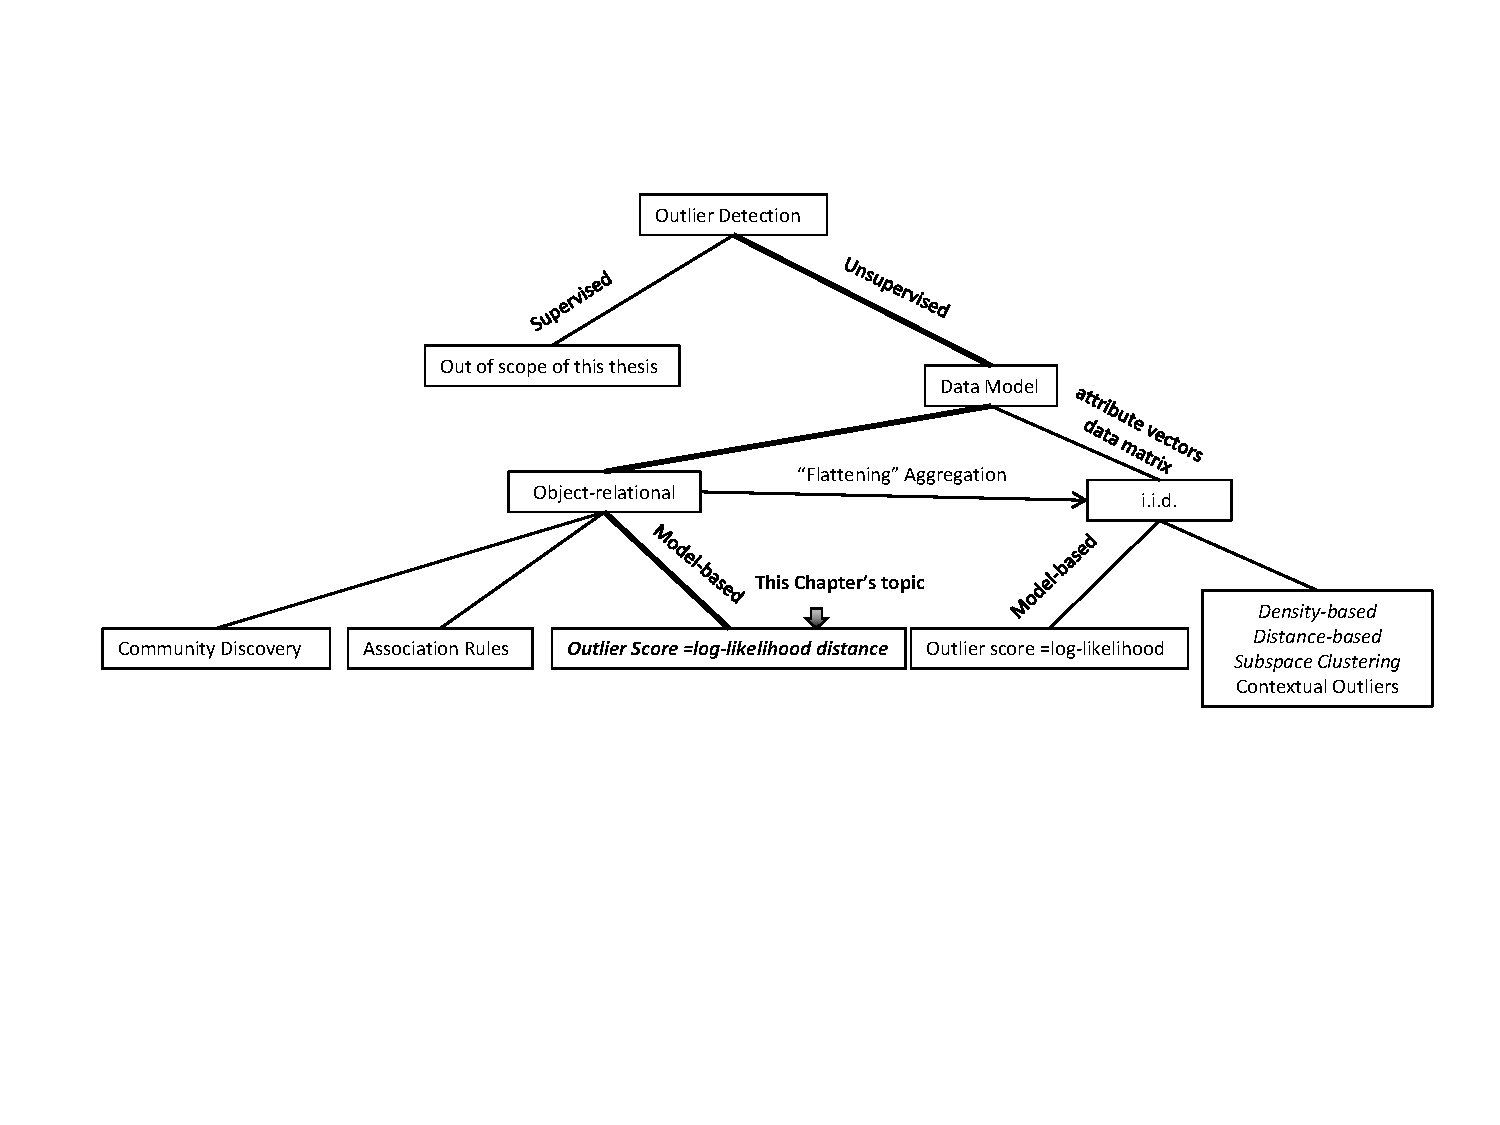
\includegraphics[width=1\textwidth] {figures/novelty-sep.pdf}
		\caption{A tree structure for related work on outlier detection for structured data. A path specifies an outlier detection problem, the leaves list major approaches to the problem. Approaches in italics appear in experiments.
			\label{fig:novelty}}
	\end{figure}
%	%\vspace{-5mm}
%	
%	\textit{b) Structured Data Models:} We discuss related techniques in three types of structured data models: SQL (relational), XML (hierarchical), and OLAP (multi-dimensional). 
%	
%	For relational data, many outlier detection approaches aim to discover rules that represent the presence of anomalous associations for an individual or the absence of normal associations \cite{Maervoet2012,Gao2010}. The survey by \cite{Novak2009} unifies within a general rule search framework related tasks such as exception mining, which looks for associations that characterize unusual cases, subgroup mining, which looks for associations  characterizing important subgroups, and contrast space mining, which looks for differences between classes. Another rule-based approach uses Inductive Logic Programming techniques \cite{Angiulli2007}.
%	%,Angiulli2009}.
%	While local rules are informative, they are not based on a global statistical model and do not provide a single outlier score for each individual. 
%	
%	A latent variable approach in information networks ranks potential outliers in reference to the latent communities inferred by network analysis \cite{Gao2010}. Our model aggregates information from entities and links of different types, but does not assume that different communities have been identified. 
%	
%	
%	Koh {\em et al.}~\cite{koh2008} propose a method for hierarchical structures represented in XML document trees. Their aim is to identify feature outliers, not class outliers as in our work. Also, they use aggregate functions to convert the object hierarchy into feature vectors. Their outlier score is based on local correlations, and they do not construct a model.
%	
%	
%	The multi-dimensional data model defines numeric measures for a set of dimensions. 
%	%A seminal approach to exploring a multi-dimensional datacube was presented by Sarawagi {\em et al.}~\cite{Sarawagi1998}. 
%	%The object and the multi-dimensional data models are similar in the respect that both objects and dimensions are ordered in a hierarchy. However, 
%	The differences in the two data models mean that multi-dimensional outlier detection models~\cite{Sarawagi1998} do not carry over to object-relational outlier detection. (1) The object data model allows but does not require any numeric measures. In our datasets, all features are discrete. Nor do we assume that it is possible to aggregate numeric measures to summarize lower-level data at higher levels.  
%	(2) In scoring a potential outlier object, our method considers other objects {\em both} below and above the target object in the component hierarchy. OLAP exploration methods consider only cells below or at the same level as the target cell. For example, in scoring a player, our method would consider features of the player's team.  
%	Also, our proposed outlier score of an object is not determined by the outlier scores of its components, in contrast to the approach of Sarawagi {\em et al.}~\cite{Sarawagi1998}.
%	% They use values such as the most unusual cell that is below a target cell.
%	(3) Our approach models a joint distribution over features, exploiting correlations among features. Most of the OLAP-based methods consider only a single numeric measure at a time, not a joint model.  
%	\section{Background: Bayesian Networks for Relational Data}
%	We adopt  
%	the Parametrized Bayes net (PBN) formalism \cite{Poole2003} that combines Bayes nets with logical syntax for expressing relational concepts. 
%	
%	
%	\subsection{Bayesian Networks}
%	
%	A {\bf Bayesian Network (BN) structure} $\model$ is a directed acyclic graph (DAG)  whose nodes comprise a set of random variables \cite{Pearl1988}. Depending on context, we interchangeably refer to the nodes  and variables of a BN. Fix a set of variables $\Features = \{\feature_{1},\ldots,\feature_{n}\}$. 
%	%These are attributes of objects, which can and typically do belong to different classes. In statistical terms, each attribute defines a random variable. 
%	The possible values of $\feature_{i}$ are enumerated as $\{\nodevalue_{i1},\ldots,\nodevalue_{i\states_{i}}\}$. The notation $P(\feature_{i} = \nodevalue)\equiv P(\nodevalue)$ denotes the probability of variable $\feature_{i}$ taking on value $\nodevalue$. We also use the vector notation $P(\Features = \set{\nodevalue}) \equiv P(\set{\nodevalue})$ to denote the joint probability that each variable $\feature_{i}$ takes on value $\set{\nodevalue}_{i}$. 
%	
%	
%	The conditional probability parameters of a Bayesian network specify the distribution of a child node given an assignment of values to its parent node. For an assignment of values to its nodes, a BN defines the joint probability as the product of the conditional probability of the child node value given its parent values, for each child node in the network. This means that the log-joint probability can be {\em decomposed} as the node-wise sum
%	
%	\begin{equation} \label{eq:bn}
%	\ln P(\Features = \set{\nodevalue};\model,\parameters) = \sum_{i=1}^{n} \ln \parameter(\set{\nodevalue}_{i}|\set{\nodevalue}_{\parents_{i}})
%	\end{equation}
%	
%	where $\set{\nodevalue}_{i}$ resp. $\set{\nodevalue}_{\parents_{i}}$ is the assignment of values to node $\feature_{i}$ resp. the parents of $\feature_{i}$ determined by the assignment $\set{\nodevalue}$. 
%	%The function $\ln$ is the binary logarithm base 2. 
%	To avoid difficulties with $\ln(0)$, here and below we assume that joint distributions are positive everywhere. Since the parameter values $\parameters$ for a Bayes net define a joint distribution over its nodes, they therefore entail a marginal, or unconditional, probability for a single node. We denote the \textbf{marginal probability} that node $\feature$ has value $\nodevalue$ as $P(\feature = \nodevalue;\model,\parameters) \equiv \parameter(\nodevalue)$. In the following we use the term Bayesian network model to refer to a network structure with parameters (i.e., a pair $(\model,\parameters)$); for brevity, we also use the terms ``Bayesian network'' or ``model''. 
%	
%	\paragraph{Example.} Figure~\ref{fig:bns} shows an example of a Bayesian network model and associated joint and marginal probabilities.
%	%
%	%\footnote{\textbf{Sarah}: add marginal probability P(res=win) for object parameters}
%	\begin{figure}[t]
%		\centering
%		\includegraphics[width=1\textwidth] 
%		{figures/bnuncropped}
%		\caption{Example of joint and marginal probabilities computed from a toy Bayesian network structure. The parameters were estimated from the  Premier League dataset. (Top): A class model Bayesian network $\model_{\class}$ for all teams with class parameters $\parameters_{\class}$. (Bottom): The same Bayesian network structure with object parameters $\parameters_{\object}$ learned for Wigan Athletics ($T = WA$). Our model-based methods outlier scores compare the data likelihood of the class parameters and the object parameters.
%			%We show only the Markov blanket of the Results node to simplify. 
%			\label{fig:bns}
%		}
%	\end{figure}
	
	
%	\begin{figure}[t]
%		\centering
%		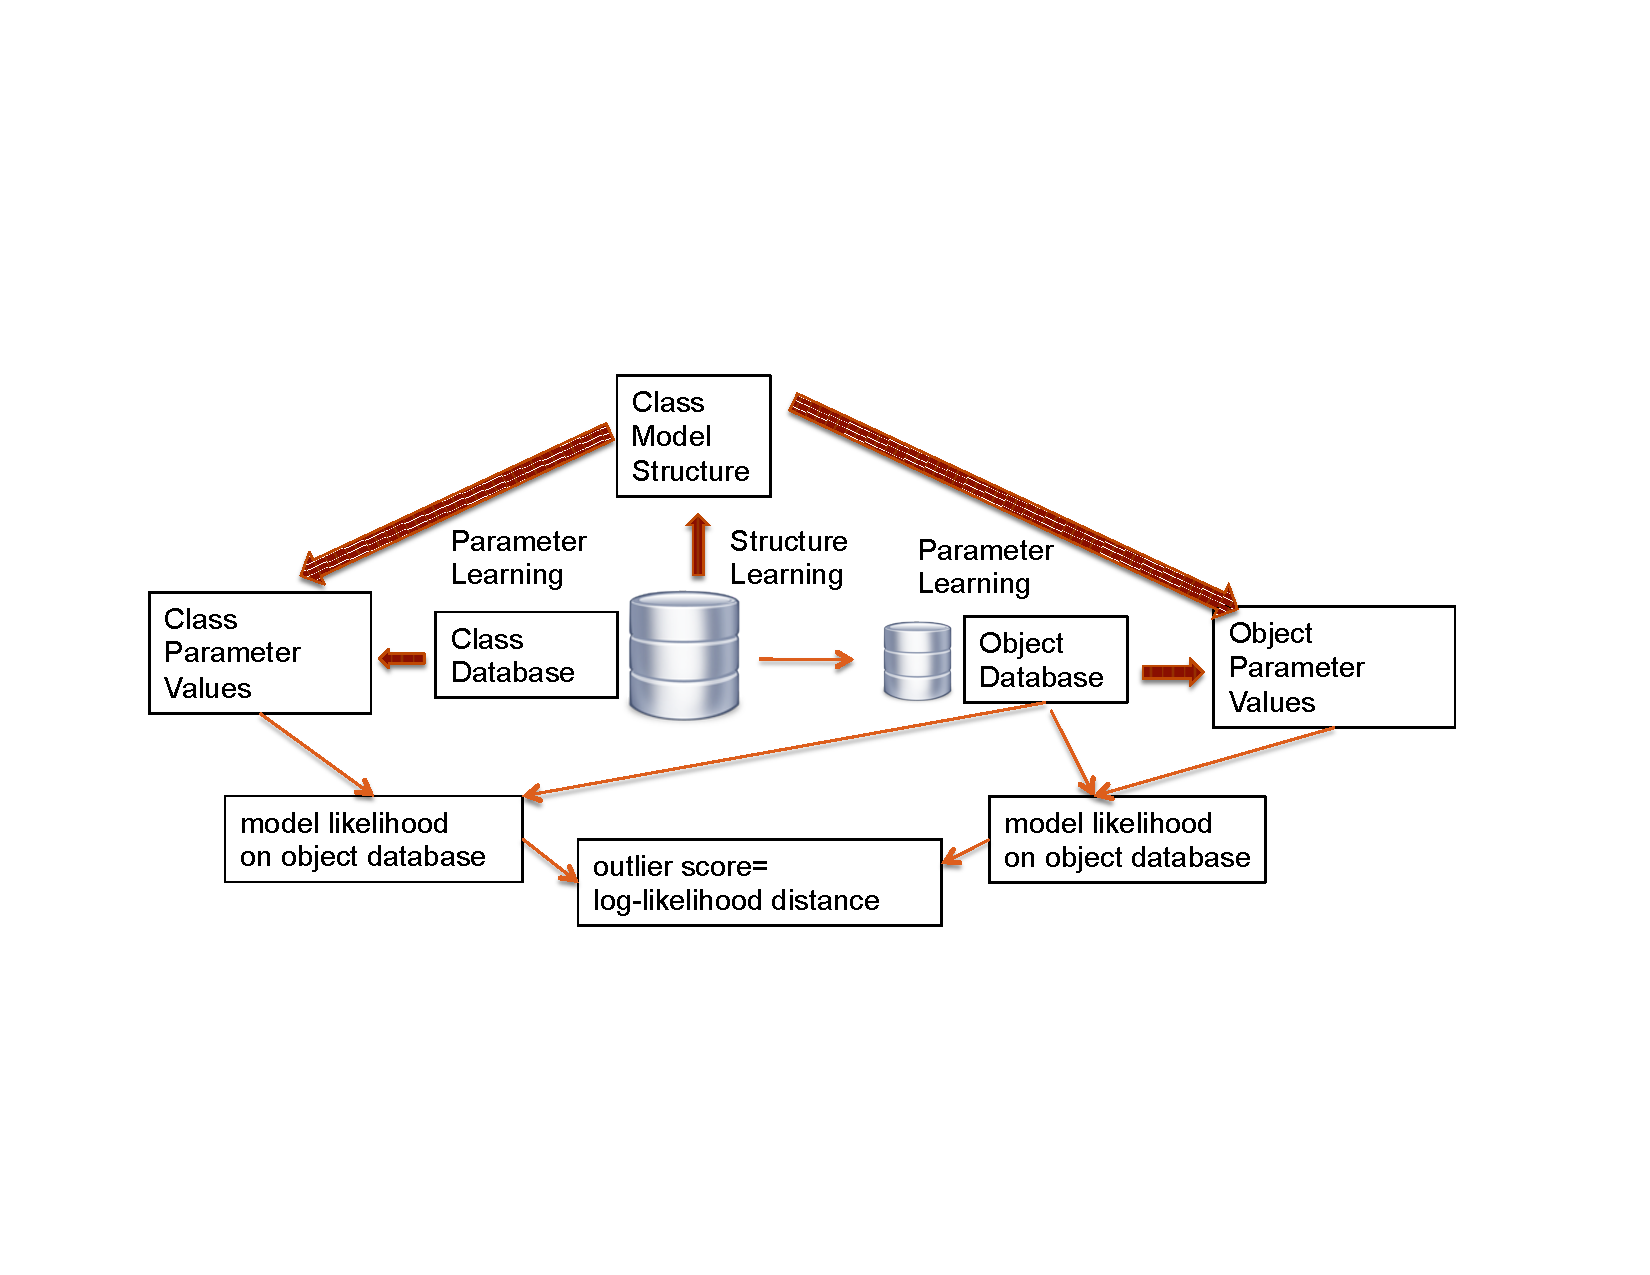
\includegraphics[width=1\textwidth]{figures/flow.pdf}
%		
%		\caption{Computation of outlier score. 
%			\label{fig:flow}}
%	\end{figure}
	%				\begin{figure}
	%				\centering
	%				\resizebox{0.9\textwidth}{!}{
	%				
	%				\subfigure{
	%				  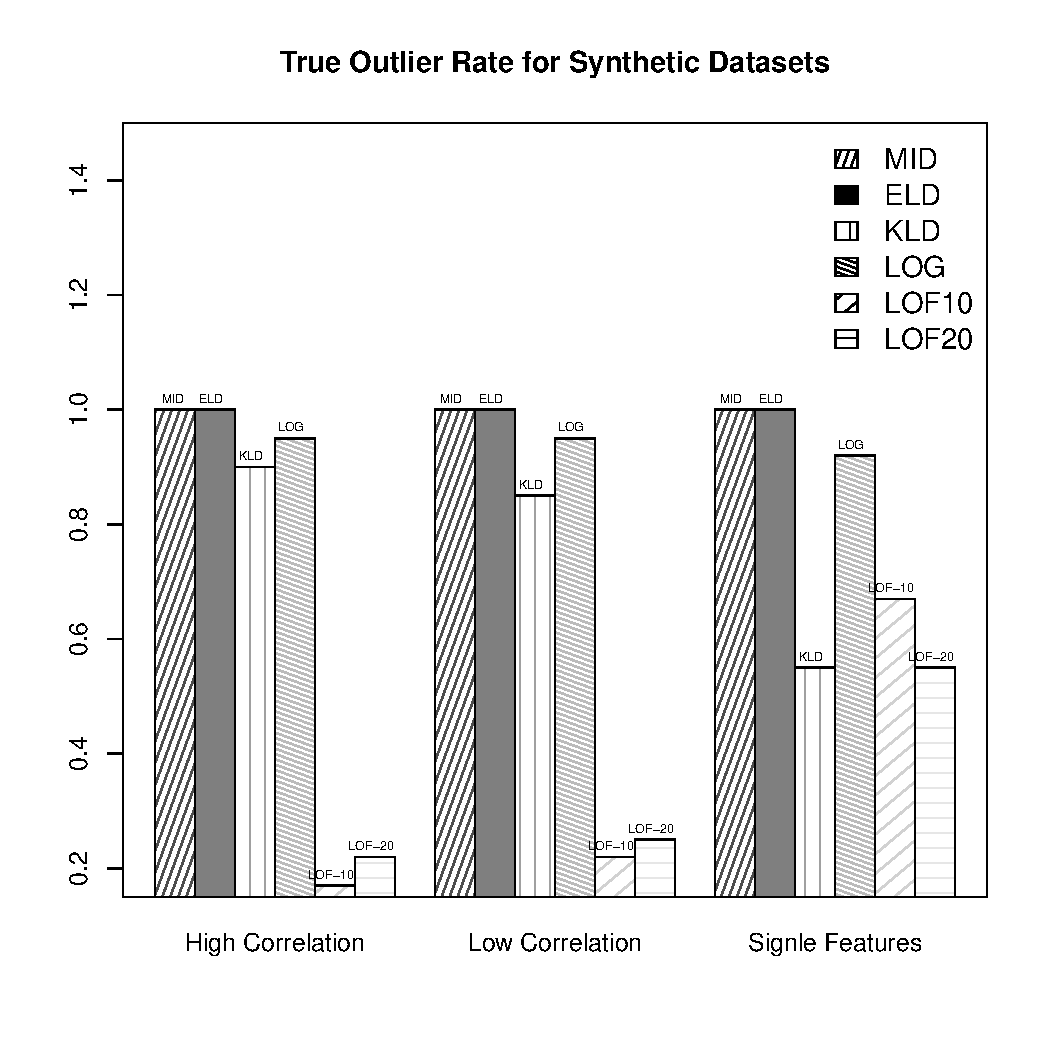
\includegraphics[height=70mm, width=70mm] {figures/TPR-Synthetic.pdf}
	%				}
	%				\subfigure{
	%				  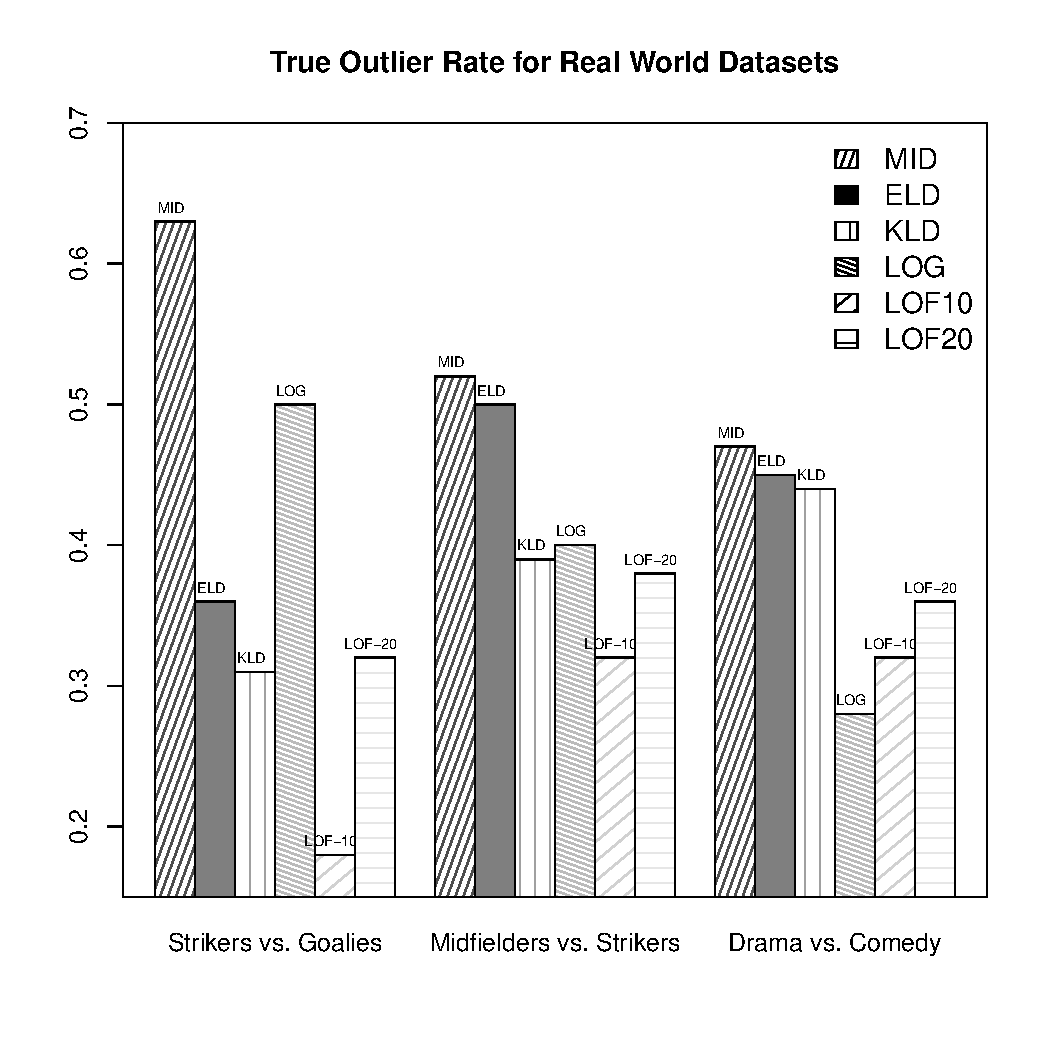
\includegraphics[height=70mm, width=70mm] {figures/TPR-All.pdf}
	%				
	%				 }
	%				 }
	%				
	%				\caption{Comparison of Object Outlier Metrics}
	%				\label{fig:synthetic}
	%				\end{figure}
	%				
	
	%				\begin{figure}
	%					\centering
	%					\begin{subfigure}{0.4\textwidth}
	%						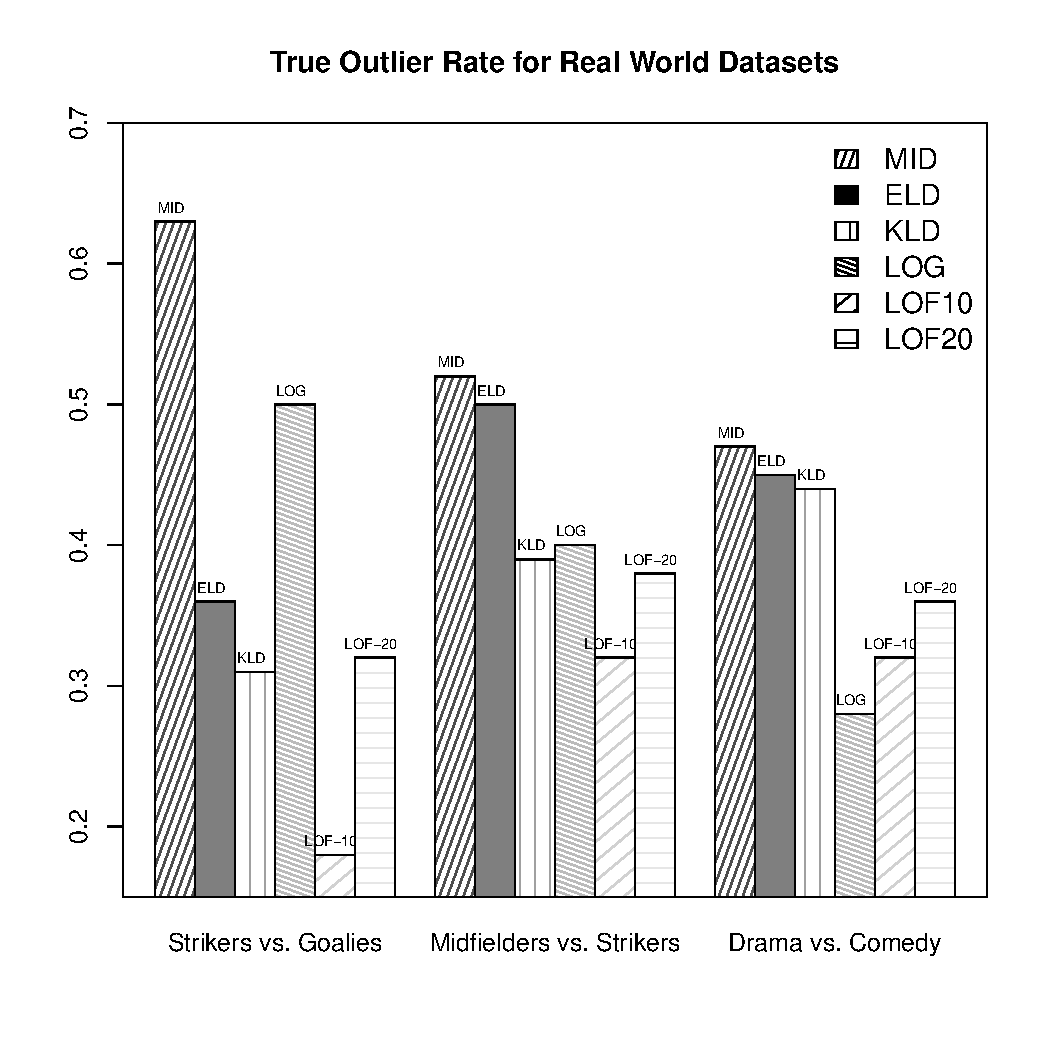
\includegraphics[width=1\linewidth]{figures/TPR-All.pdf}
	%						\caption{}
	%						\label{fig:Ng1} 
	%					\end{subfigure}
	%					
	%					\begin{subfigure}{0.4\textwidth}
	%						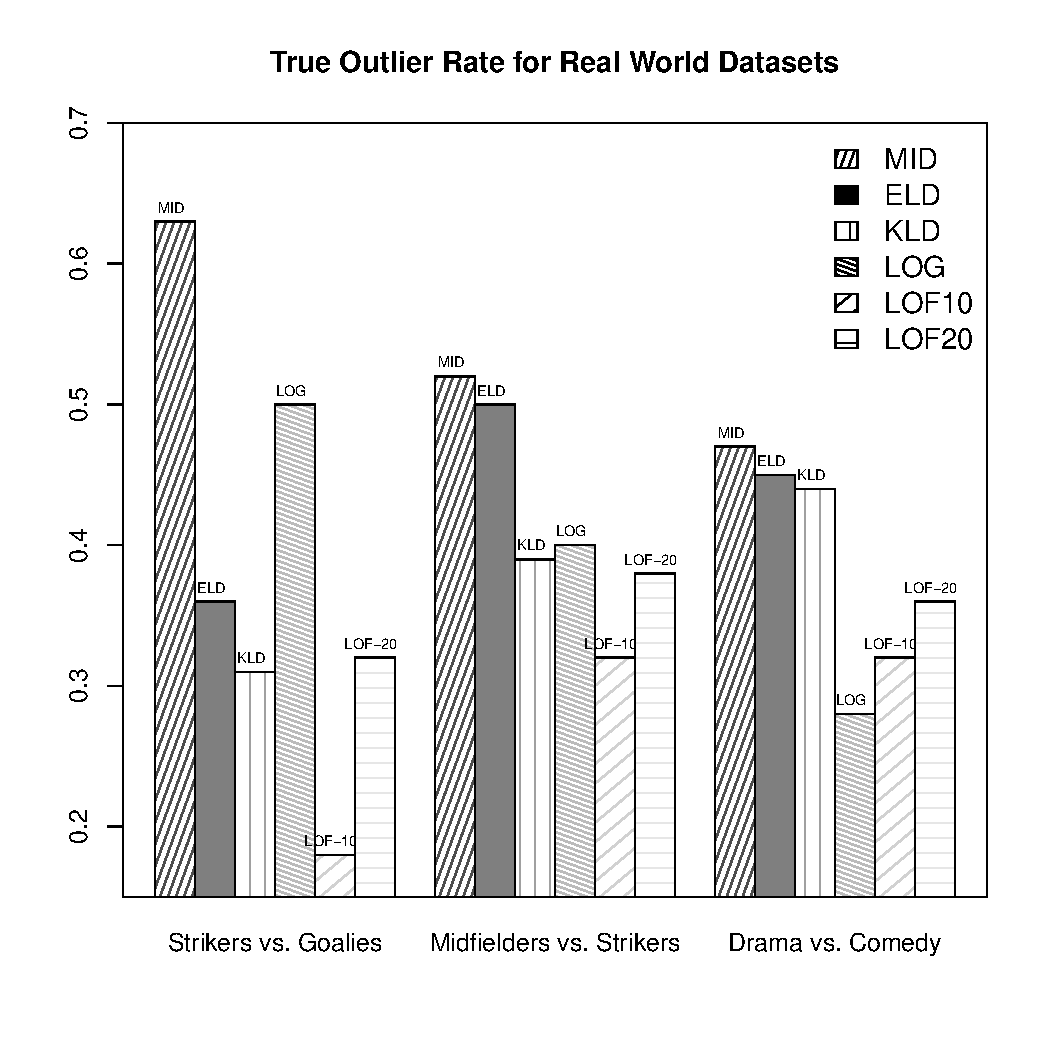
\includegraphics[width=1\linewidth]{figures/TPR-All.pdf}
	%						\caption{}
	%						\label{fig:Ng2}
	%					\end{subfigure}
	%					
	%					\caption[Two numerical solutions]{(a) Numerical solutions for the small-time system 
	%						with a constant-curvature body shape showing the scaled leading-order veritcal 
	%						reaction force $N_0$ versus the scaled body mass $M$ for various values of $g$. 
	%						Again, $I=M$ for definiteness and $A=0.7$. (b) As for (a) but over a wider range of 
	%						values of $M,I$.}
	%				\end{figure}
	
%	\subsection{Relational Data}
%	
%	
%	
%	
%	%We apply the learn-and-join algorithm (LAJ), which is the state-of-the-art Bayes net learning method for relational data. The LAJ algorithm takes as input a relational database and outputs a Bayes net using the functor notation due to Poole \cite{Poole2003}. We briefly review this notation.
%	
%	%\paragraph{Functor Terms} 
%	We adopt a term-based notation for combining logical and statistical concepts~\cite{Poole2003,Kimmig2014}.
%	A functor is a function or predicate symbol. Each functor has a set of values (constants) called the \textbf{domain} of the functor. The domain of a \textbf{predicate} is $\{\true,\false\}$. Predicates are usually written with uppercase Roman letters, other terms with lowercase letters.
%	A predicate of arity at least two is a \textbf{relationship} functor. Relationship functors specify which objects are linked. Other functors represent \textbf{features} or \textbf{attributes} of an object or a tuple of objects (i.e., of a relationship).
%	A \textbf{population} is a set of objects. 
%	A \textbf{term} is of the form $f(\term_{1},\ldots,\term_{k})$ where $\functor$ is a functor %(either a function symbol or a predicate symbol) 
%	and each $\term_{i}$ is a first-order variable or a constant denoting an object. A term is \textbf{ground} if it contains no first-order variables; otherwise it is a first-order term. In the context of a statistical model, we refer to first-order terms as \textbf{Parametrized Random Variables} (PRVs) \cite{Kimmig2014}. 
%	%A term whose range are the truth values $\{\true,\false\}$ is a \textbf{predicate}. 
%	%Predicates are usually written with uppercase Roman letters, other term with lowercase letters.
%	%The grounding concept represents moving from the population-level  to the object level. 
%	A \textbf{grounding} replaces each first-order variable in a term by a constant; the result is a ground term. A grounding may be applied simultaneously to a set of terms.  A relational database $\D$ specifies the values of all ground terms. %, which can be listed in data tables. 
%	%In machine learning terminology, the data tables are contingency tables that represent sufficient statistics or event counts.
%	
%	Consider a joint assignment 
%	$P(\Features = \set{\nodevalue})$ of values to a set of PRVs $\Features$. The {\em grounding space} of the PRVs is the set of all possible grounding substitutions, each applied to all PRVs in $\Features$. The {\em count} of groundings that satisfy the assignment with respect to a database $\D$ is denoted by $\grounds_{\D}(\Features = \set{\nodevalue})$. The \textbf{database frequency} $P_{\D}(\Features = \set{\nodevalue})$ is the grounding count divided by the number of all possible groundings. 
%	%, that is, the size of the grounding space.
%	
%	\emph{Example.} \label{sec:example}
%	%
%	The Opta dataset represents information about Premier League data %\cite{opta-original} 
%	(Sec.~\ref{sec:real-world-data}). 
%	%Using the functor notation, the data
%	%format can be represented as follows. 
%	The basic populations are teams, players, matches, with 
%	corresponding first-order variables $\team, \player, \match$. As shown in Table~\ref{table:data}, the groundings count can be visualized in terms of a groundings table ~\cite{Schulte2012}, also called a universal schema~\cite{Riedel2013}. 
%	%Table~\ref{table:data} specifies values for some ground terms. 
%	The first three column headers show first-order variables ranging over different populations. The remaining columns represent terms. Each row represents a single grounding and the values of the ground terms defined by the grounding.
%	%Table~\ref{table:counts} illustrates grounding counts. 
%	In terms of the grounding table, the grounding count of a joint assignment is the number of rows that satisfy the conditions in the joint assignment. The database frequency is the grounding count, divided by the total number of rows in the groundings table. Counts are based on the 2011-2012 Premier League Season. We count only groundings $(\it{team},\it{match})$ such that $\it{team}$ plays in $\it{match}$. Each team, including Wigan Athletics, appears in 38 matches. The total number of team-match pairs is $38 \times 20 = 760$.
%	
	%Examples of terms include the following. 
	
	%\begin{itemize}
	%\item $\it{Appears\_Player}(\P,\M)$ indicates whether a player appeared in a match.
	%\item $\it{Appears\_Team}(\T,\M)$ indicates whether a team played in a match.
	%\item $\it{Team}(\P)$ returns the team of a player.
	%\item $\it{Result}(\T,\M)$ denotes the result of a team in a match (win or lose).
	%\item $\it{ShotEff}(\T,\M)$ denotes the shot efficiency of a team in a match (number of successful shots on target, per total number of shots).
	%\item $\it{TimePlayed}(\P,\M)$ denotes the total time that a player played in a match.
	%\end{itemize}
	
	
	%\begin{table}[htbp]
	%\caption{Examples of terms in the soccer dataset.}
	%\centering
	%\resizebox{1\textwidth}{!}{
	%\begin{tabular}{|c|p{5cm}|}
	%\hline
	%Term&Meaning\\ \hline
	%$\it{Appears\_Player}(\P,\M)$ & indicates whether a player appeared in a match.\\ \hline
	%$\it{Appears\_Team}(\T,\M)$&indicates whether a team played in a match.\\ \hline
	%$\it{Team}(\P)$& returns the team of a player.\\ \hline
	%$\it{Result}(\T,\M)$ &denotes the result of a team in a match (win or lose).\\ \hline
	%$\it{ShotEff}(\T,\M)$ &denotes the shot efficiency of a team in a match (number of successful shots on target, per total number of shots).\\ \hline
	%$\it{TimePlayed}(\P,\M)$& denotes the total time that a player played in a match.\\ \hline
	%\end{tabular}}
	%\label{table:terms}
	%\end{table}
	
%	\begin{table}[htbp]
%		\caption{Sample Population Data Table (Soccer). \label{table:data}}
%		\centering
%		\resizebox{1\textwidth}{!}{
%			\begin{tabular}{|c|c|l|c|c|c|c|}
%				\hline
%				\multicolumn{1}{|l|}{MatchId \match} &
%				TeamId \team & PlayerId \player& \multicolumn{1}{l|}{First\_goal(\player,\match)} 
%				& \multicolumn{1}{l|}{TimePlayed(\player,\match)} & 
%				\multicolumn{1}{l|}{ShotEff(\team,\match)}&result(\team,\match) \\ \hline
%				117 & WA & McCarthy & 0 & 90 & 0.53&\it{win}\\ \hline
%				148 & WA & McCarthy & 0 & 85 & 0.57&\it{loss}\\ \hline
%				15 & MC & Silva & 1 & 90 & 0.59&\it{win}\\ \hline
%				\ldots& \ldots &\ldots&\ldots&\ldots&\ldots&\\
%			\end{tabular}}
%			\caption{Sample Object Data Table, for team $\team = \it{WA}$. \label{table:individual}}
%			\resizebox{1\textwidth}{!}{
%				\begin{tabular}{|c|c|l|c|c|c|c|}
%					\hline
%					\multicolumn{1}{|l|}{MatchId \match} &
%					TeamId $\team = \it{WA}$ & PlayerId \player& \multicolumn{1}{l|}{First\_goal(\player,\match)} 
%					& \multicolumn{1}{l|}{TimePlayed(\player,\match)} & 
%					\multicolumn{1}{l|}{ShotEff(\it{WA},\match)}&result(\it{WA},\match) \\ \hline
%					117 & WA & McCarthy & 0 & 90 & 0.53&\it{win}\\ \hline
%					148 & WA & McCarthy & 0 & 85 & 0.57&\it{loss}\\ \hline
%					\ldots& WA &\ldots&\ldots&\ldots&\ldots&\\
%				\end{tabular}}
%			\end{table}
%			
%			
%			
%			
%			A novel aspect of our work is that we learn model parameters for specific objects as well as for the entire population. 
%			%To implement this, for each target object, we form 
%			The appropriate \textbf{object data table} is formed from the population data table by restricting the relevant first-order variable to the target object. 
%			For example, the object database for target Team $\it{Wigan Athletic}$, 
%			forms a subtable of the data table of Table~\ref{table:data} that contains only rows where 
%			TeamID = $\it{WA}$; see Table~\ref{table:individual}. In database terminology, an object database is like a view centered on the object. %[The object database is an individual-centered representation \cite{Flach1999a}. move to related work.]
			
			%\begin{table} 
			%	\captionsetup{singlelinecheck=off}
			%			\caption[.]{\label{table:counts}Example of Grounding Count and Frequency for the conjunction \begin{displaymath} \it{passEff(T,M)=hi}, shotEff(T,M)=high, Result(T,M)=1.\end{displaymath}}
			%			\centering
			%			\resizebox{1\textwidth}{!}{
			%				\begin{tabular}{|c|c|c|}
			%					\hline
			%					Database&Count or $\#_{D}(\Features = \set{\nodevalue})$&Frequency or $P_{D}(\Features = \set{\nodevalue})$\\\hline
			%					Population&76& $76/760=0.10$\\\hline
			%					Wigan Athletics&7&$7/38=0.18$\\\hline
			%		
			%					%Synthetic&40&280\\ \hline
			%				\end{tabular}}
			%			\end{table}
			\begin{table} 
				\caption{Example of grounding count and frequency in the Premier League data, for the conjunction $\it{passEff(T,M)=hi}, shotEff(T,M)=hi, Result(T,M)=win$.\label{table:counts}}
				\centering
				\resizebox{1\textwidth}{!}{
					\begin{tabular}{|c|c|c|}
						\hline
						Database&Count or $\#_{D}(\Features = \set{\nodevalue})$&Frequency or $P_{D}(\Features = \set{\nodevalue})$\\\hline	A novel aspect of our paper is that we learn model 
						Population&76& $76/760=0.10$\\\hline                                                                               	A novel aspect of our paper is that we learn model 
						Wigan Athletics&7&$7/38=0.18$\\\hline
						
						%Synthetic&40&280\\ \hline
					\end{tabular}}
				\end{table}
				
				%\begin{table} 
				%	\captionsetup{singlelinecheck=off}
				%			\caption[.]{\label{table:counts}Example of Grounding Count and Frequency for the conjunction \begin{displaymath} \it{passEff(T,M)=hi}, shotEff(T,M)=high, Result(T,M)=1.\end{displaymath} Counts are based on the 2011-2012 Premier League Season. We count only groundings $(\it{team},\it{match})$ such that $\it{team}$ plays in $\it{match}$. Each team, including Wigan Athletics, appears in 38 matches. The total number of team-match pairs is $38 \times 20 = 760$.
				%			\label{MetricComputation}}
				%			\centering
				%			\resizebox{1\textwidth}{!}{
				%				\begin{tabular}{|c|c|c|}
				%					\hline
				%					Database&Count or $\#_{D}(\Features = \set{\nodevalue})$&Frequency or $P_{D}(\Features = \set{\nodevalue})$\\\hline
				%					Population&76& $76/760=0.10$\\\hline
				%					Wigan Athletics&7&$7/38=0.18$\\\hline
				%		
				%					%Synthetic&40&280\\ \hline
				%				\end{tabular}}
				%				
				%			\end{table}
				
				%[Example of counts, frequencies]
				% For simplicity only, suppose that the only matches and players in the season are those shown in Table~\ref{table:data}. Then the attribute value $\it{First\_goals} = 0$ occurs with frequency $1/2$ in the object distribution $P_{\it{si}}$ for Silca. In the player class distribution $P_{\it{Player}}$, the attribute value $\it{First\_goals} = 0$ occurs with frequency $4/5$. So Silva is somewhat less likely to score no goal than a randomly selected player.
			%	\subsection{Bayesian Networks for Relational Data}
				
		%		A \textbf{Parametrized Bayesian Network Structure} (PBN) is a Bayesian network structure  whose nodes are PRVs~\cite{Poole2003}. 
				%For most of the paper we refer to PBNs simply as Bayesian networks, and to PRVs simply as random variables. 
				%The learn-and-join algorithm is the state-of-the-art Bayes net learning method for relational data, based on model search in the lattice of relationship joins \cite{Schulte2012}. The LAJ algorithm takes as input a relational database and outputs a Parametrized Bayes net structure.
				%We review the algorithm very briefly; for further details please see \cite{Schulte2012}. 
				%The algorithm builds a Bayes net for an entire database by level-wise search through the {\em lattice of relationship chains.} This is the lattice of relationship sets that are connected by shared first-order variables.
				%%; see Figure~\ref{fig:lattice}.  
				%%We describe the fundamental ideas of the algorithm; for further details please see \cite{Schulte2012}. 
				%The user chooses a single-table Bayes net learner. The learner is applied to base population data tables. Then the learner is applied to data tables for relationship chains of size $s,s+1,\ldots$, with the constraint that the models for larger join tables inherit the absence or presence of learned edges from smaller join tables. 
				%
%				The relationships and features in an object database define a set of nodes for Bayes net learning.%; see Figure~\ref{fig:bns}.
				% shows a sample PBN.
				
				
				%We use the following notation.
				
				%\begin{figure}[ht]
				%\centering
				%   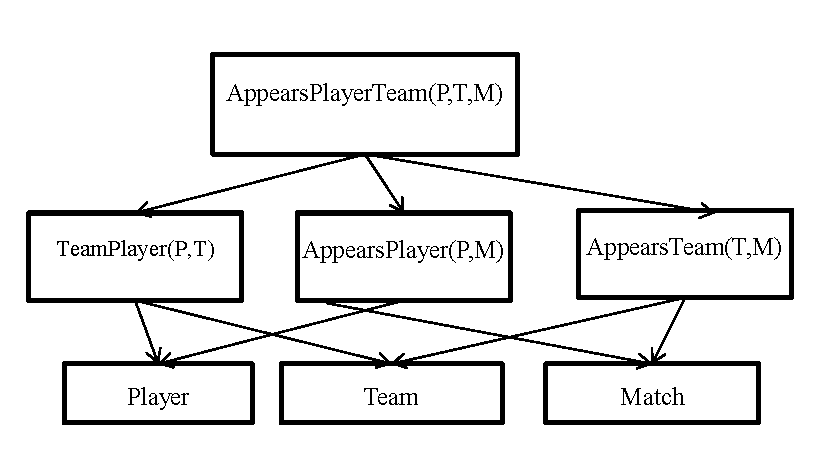
\includegraphics[width=0.3\textwidth] {lattice}
				% \caption{Lattice of Premier League dataset.
				% %We show only the Markov blanket of the Results node to simplify. 
				% \label{fig:lattice}}
				%\end{figure}
				
				
				
				
				%\begin{itemize}
				%\item $\D_{\population}$ is the database for the entire population; cf. Table~\ref{table:data}.
				%\item $\D_{\target}$ is the restriction of the input database to the target object; cf. Table~\ref{table:object}. 
				%\item $\M_{\population}$ is a model (e.g., Bayesian network) learned with $\D_{\population}$ as the input database; cf. Figure~\ref{fig:bns}(a).
				%\item $\M_{\target}$ is an object model (e.g., Bayesian network) learned with $\D_{\target}$ as the input database; cf. Figure~\ref{fig:bns}(b).
				%\end{itemize}
				%
				
				\subsubsection{Model Likelihood for Parametrized Bayesian Networks}
				
				
%					***	A novel aspect of our work is that we learn model parameters for specific objects as well as for the entire population. 
				
				A standard method for applying a generative model assumes that the generative model represents normal behavior since it was learned from the entire population. An object is deemed an outlier if the model assigns sufficiently low likelihood to generating its features \cite{Cansado2008}. This likelihood method is an important baseline for our investigation.
				%, so we define the likelihood function formally in this section. 
				%The other outlier scores we consider can be viewed as improved variants of the likelihood approach. 
				Defining a likelihood for relational data is more complicated than for i.i.d. data because an object is characterized not only by a feature vector, but by an object  database.
				% that lists the object's links and the attributes of linked entities. 
				%For the model likelihood function $\lnlikelihood(\model,\D)$, where $\model$ denotes a Bayesian network, 
				We employ the relational pseudo log-likelihood \cite{Schulte2011}, which can be computed as follows for a given Bayesian network  and database.
				
				%\begin{eqnarray}
				%\lnlikelihood(\model,\D) =   \sum_{i=1}^{n}\sum_{j=1}^{\states_{i}} \sum_{\parents_{i}}\\ P_{\D}(\feature_{i} = \nodevalue_{ij},\parents_{i})\ln \parameter_{\model}(\feature_{i} = \nodevalue_{ij}|\parents_{i})  \nonumber
				%\end{eqnarray}
				
				\begin{equation} \label{eq:likelihood}
				\loglikelihood(\D,\model,\parameters) =   \sum_{i=1}^{n}\sum_{j=1}^{\states_{i}} \sum_{\parents_{i}}\P_{\D}(\nodevalue_{ij},\parents_{i})\ln \parameter(\nodevalue_{ij}|\parents_{i})  
				\end{equation}
				
				
				Equation~\eqref{eq:likelihood} represents the standard BN log-likelihood function for the object  data~\cite{Campos2006}, except that parent-child instantiation counts are standardized to be proportions \cite{Schulte2011}. The equation can be read as follows.
				
				\begin{enumerate}
					\item For each parent-child configuration, 
					use the conditional probability of the child given the parent.
					\item Multiply the logarithm of the conditional probability by the database frequency of the parent-child configuration. 
					%The instantiation proportion is the number of instantiating groundings, divided by the total number of possible instantiations.
					\item Sum this product over all parent-child configurations and all nodes. 
				\end{enumerate}
				
				%\begin{eqnarray}
				%\lnlikelihood&   \sum_{i=1}^{n}\sum_{j=1}^{\states_{i}} \sum_{\parents_{i}} P_{\D}(\feature_{i} = \nodevalue_{ij},\parents_{i})\ln \parameter_{\model}(\feature_{i} = \nodevalue_{ij}|\parents_{i})
				%\end{eqnarray}
				
				The maximum of the pseudo-likelihood ~\eqref{eq:likelihood} is given by the empirical database frequencies \cite[Prop.3.1.]{Schulte2011}. In all our experiments we use these maximum likelihood parameter estimates.
				
				{\em Example.} The family configuration \begin{displaymath} \it{passEff(T,M)=hi}, shotEff(T,M)=hi, Result(T,M)=win\end{displaymath} contributes one term to the pseudo log-likelihood for the BN Figure 3.3 of chapter~\ref{chap:three}. For the population database, this term is $0.1 \times \ln(0.44) =-0.08 $. For the  Wigan Athletics database, the term is $0.18 \times \ln(0.44) =-0.14 $. 

	\section{Likelihood-Distance Object Outlier score} \label{sec:metrics}
	
	We introduce a novel model-based outlier score, that extends the log-likelihood~\eqref{eq:likelihood}, using the following notation.
	\begin{itemize}
		\item $\D_{\Class}$ is the database for the entire class of objects; cf. Table 3.1 of chapter~\ref{chap:three}. This database defines the \textbf{class distribution} $P_{\Class} \equiv P_{\D_{\class}}$.
		\item $\D_{\object}$ is the restriction of the input database to the target object; cf. Table 3.2 of chapter~\ref{chap:three}. This database defines the \textbf{object distribution} $P_{\object} \equiv P_{\D_{\object}}$.
		\item $\model_{\Class}$ is a Bayesian network structure learned with $\D_{\population}$ as the input database; cf. Figure 3.3(a) of chapter~\ref{chap:three}.
		\item $\parameters_{\Class}$ resp. $\parameters_{\object}$ are parameters learned for $\model_{\Class}$ using $\D_{\class}$ resp. $\D_{\object}$ as the input database.
	\end{itemize}
	
	Figure~\ref{fig:flow} illustrates these concepts and the system flow for computing an outlier score. First, we learn a Bayesian network structure $\model_{\Class}$ for the entire population using a previous learning algorithm (see section~\ref{sec:methods} below). We then evaluate {\em how well the class model fits the target object data.} For vectorial data, the  standard model fit metric %approach 
	is the log-likelihood of the target {\em datapoint}. For relational data, the counterpart is the relational log-likelihood \eqref{eq:likelihood} of the target {\em database}:
	
	\begin{equation} \label{eq:loglikelihood-score}
	\loglikelihood(\D_{\object},\model_{\Class},\parameters_{\Class}).
	\end{equation}
	
	
	
	While this
	%the log-likelihood~\eqref{eq:loglikelihood-score} 
	is a good baseline outlier score, it can be improved by considering scores based on the likelihood ratio, or {\bf log-likelihood difference}:
	%. The log-likelihood difference is defined by
	
	\begin{equation} \label{eq:log-diff}
	\lr(\D_{\object},\model_{\Class},\parameters_{\object}) \equiv \loglikelihood(\D_{\object},\model_{\Class},\parameters_{\object}) - \loglikelihood(\D_{\object},\model_{\Class},\parameters_{\Class}).
	\end{equation}
	
	The log-likelihood difference compares  how well the class-level parameters fit the object data, vs. how well the object parameters fit the object data. In terms of the conditional probability parameters, it measures how much the log-conditional probabilities in the class distribution differ from those in the object distribution. Note that this definition applies only for relational data where an individual is characterized by a substructure rather than a ``flat'' feature vector. Assuming maximum likelihood parameter estimation, $\lr$ is equivalent to the Kullback-Leibler divergence between the class-level and object-level parameters~\cite{Campos2006}. 
	%
	While the $\lr$ score provides more outlier information than the model log-likelihood, it can be improved further by two transformations as follows. (1) Decompose the joint probability into a single-feature component and a mutual information component. (2) Replace log-likelihood differences by log-likelihood distances. The resulting score is the \textbf{log-likelihood distance} ($\mid$), which is the main novel score we propose in this paper. Formally, it is defined as follows for each feature $i$. The total score is the sum of feature-wise scores. Section~\ref{sec:divergence-examples} 
	below provides example computations.
	%In other words, we assume that model comparison scores are decomposable, which is the case for Bayesian networks. 
	
	%\begin{equation} \label{eq:log-dist}
	%\begin{array}{l}
	%\mid_{i} =\sum_{j=1}^{\states_{i}} P_{\object}(\nodevalue_{ij}) \left|\ln \frac{\parameter_{\object}( \nodevalue_{ij})}{\parameter_{\Class}( \nodevalue_{ij})}\right|+\\
	%\sum_{j=1}^{\states_{i}} \sum_{\parents_{i}} 
	%P_{\object}( \nodevalue_{ij},\parents_{i})
	%\left|\ln \frac{\parameter_{\object}( \nodevalue_{ij}|\parents_{i})}{\parameter_{\object}(\nodevalue_{ij})} - \ln \frac{\parameter_{\Class}( \nodevalue_{ij}|\parents_{i})}{\parameter_{\Class}(\nodevalue_{ij})}\right|. 
	%\end{array}
	%\end{equation}
	%We note that for a fixed object distribution $P_{\object}$, the log-likelihood distance is a proper distance metric between the class-level and the object-level parameters. 
	%The $\mid$ has two components. 
	\begin{eqnarray}
	\mid_{i} & = & \sum_{j=1}^{\states_{i}} P_{\object}(\nodevalue_{ij}) \left|\ln \frac{\parameter_{\object}( \nodevalue_{ij})}{\parameter_{\Class}( \nodevalue_{ij})}\right|+ \label{eq:fd}\\
	& & \sum_{j=1}^{\states_{i}} \sum_{\parents_{i}} 
	P_{\object}( \nodevalue_{ij},\parents_{i})
	\left|\ln \frac{\parameter_{\object}( \nodevalue_{ij}|\parents_{i})}{\parameter_{\object}(\nodevalue_{ij})} - \ln \frac{\parameter_{\Class}( \nodevalue_{ij}|\parents_{i})}{\parameter_{\Class}(\nodevalue_{ij})}\right|. \label{eq:mi}
	\end{eqnarray}
	
	%\mid_{i} =\sum_{j=1}^{\states_{i}} P_{\object}(\nodevalue_{ij}) \left|\ln \frac{\parameter_{\object}( \nodevalue_{ij})}{\parameter_{\Class}( \nodevalue_{ij})}\right|+\\
	%\sum_{j=1}^{\states_{i}} \sum_{\parents_{i}} 
	%P_{\object}( \nodevalue_{ij},\parents_{i})
	%\left|\ln \frac{\parameter_{\object}( \nodevalue_{ij}|\parents_{i})}{\parameter_{\object}(\nodevalue_{ij})} - \ln \frac{\parameter_{\Class}( \nodevalue_{ij}|\parents_{i})}{\parameter_{\Class}(\nodevalue_{ij})}\right|. 
	
	
	The first sum~\eqref{eq:fd} is the \textbf{single-feature} component, where each feature is considered independently of all others. It computes the expected log-distance with respect to  the singe feature value probabilities between the object and the class models. 
	%For example, the single-feature sum for the feature ``Goal" of Van Persie is 5/8. 
	%
	The second $\mid$ sum~\eqref{eq:mi} is the \textbf{mutual information component}, based on the mutual information among all features; it computes the expected log-distance between the object and the class models with respect to the mutual information of feature value assignments.
	%measures the expected distance in 
	%%{\em multi-variate mutual information} 
	%{\em association component} between the object and the class distributions. 
	Intuitively, the first sum measures how the models differ if we treat each feature in isolation. The second sum measures how the models differ in terms of how strongly parent and child features are associated with each other. 
	%A standard result in information theory states that a joint distribution can, without loss of information, be decomposed into a univariate distribution and the multi-variate mutual information  \cite{Witten2005}. Considering how the distributions differ in each of these two terms therefore involves no loss of information. 
	
	%$\mid$ is not symmetric between the object and the class distribution because it weights sum terms by the joint probability in  the object distribution. The lack of symmetry is a desirable feature because to assess whether an object is an outlier, we want to weight most the events that occur more frequently with the object. 
	
	\subsection{Motivation} 
	%The motivation for using log-distances %rather than log-differences 
	%is that some log-differences are positive, some negative, and cancel each other out when their sign differs. Since our goal is to assess the distinctness of an object, {\em we do not want differences to cancel out.} Fundamentally, averaging differences is appropriate when considering costs, payoffs or utilities, but not appropriate when assessing the distinctness of an object. 
	%
	The motivation for the mutual information decomposition is two-fold. 
	
	\noindent
	(1) {\em Interpretability}, which is very important for outlier detection. The single-feature components are easy to interpret since they involve no feature interactions. Each parent-child local factor is based on the average relevance of parent values for predicting the value of the child node, where relevance is measured by $$\ln \frac{\parameter(\nodevalue_{ij}|\parents_{i})}{\parameter(\nodevalue_{ij})}.$$ This relevance term  is basically the same as the widely used lift measure \cite{Tuffery2011}, therefore an intuitively meaningful quantity. The $\mid$ score compares how relevant a given parent condition is in the object data with how relevant it is in the general class. 
	
	\noindent
	(2) {\em Avoiding cancellations.} The \textbf{mutual information decomposition} shows that each term in the log-likelihood difference \eqref{eq:log-diff} decomposes into a relevance difference and a marginal difference: 
	
	\begin{equation} \label{eq:decompose}
	\ln \frac{\parameter_{\object}( \nodevalue_{ij}|\parents_{i})}{\parameter_{\Class}( \nodevalue_{ij}|\parents_{i})} = \ln \frac{\parameter_{\object}(\nodevalue_{ij}|\parents_{i})}{\parameter_{\object}(\nodevalue_{ij})} - \ln \frac{\parameter_{\Class}( \nodevalue_{ij}|\parents_{i})}{\parameter_{\Class}(\nodevalue_{ij})} + \ln \frac{\parameter_{\object}( \nodevalue_{ij})}{\parameter_{\Class}( \nodevalue_{ij})}.
	\end{equation}
	
	These differences can have different signs for different child-parent configurations and cancel each other out; see Table~\ref{table:Formula} below for an example.  Since our goal is to assess the distinctness of an object, {\em we do not want differences to cancel out.} Taking distances ,as in Equations~\eqref{eq:fd} and ~\eqref{eq:mi}, avoids the undesirable cancellation. The general point is that averaging differences is appropriate when considering costs, or utilities, but not appropriate for assessing the distinctness of an object. For instance, the average component-wise difference of the vectors (0,0) and (1,-1) is 0, but their distance is not.
	
	
		\subsection{Comparison Outlier Scores} \label{sec:comparison} Our lesion study compares our log-likelihood distance  $\mid$ score to baselines that are defined by omitting a component of $\mid$. In this section we define these scores.
		%and provide a theoretical comparison. 
		The scores increase in sophistication in the sense that they apply more transformations of the log-likelihood ratio. 
		%Our empirical comparison below indicates that the 
		More sophisticated scores provide more information about outliers.   
		%defines the scores formally.  
		Table~\ref{table:Formula} defines local feature scores; the total score is the sum of feature-wise scores. All metrics are defined such that {\em a higher score indicates a greater anomaly.} The metrics are as follows. 
		
		\begin{description}
			\item[Feature Divergence $\fd$] is the first  component of the $\mid$ score. It considers each feature independently (no feature correlations).
			%							
			\item[Log-Likelihood Score \loglikelihood] is the standard model-based outlier detection score using data likelihood.
			\item[Log-Likelihood Difference \lr] is the log-likelihood difference~\eqref{eq:log-diff} between the class-level and object-level parameters. %(Equation). 
			\item[Log-Likelihood Difference with absolute value $|\lr|$] replaces differences in $\lr$ by distances.
%			\item[Log-Likelihood Difference with decomposition $\lr^{+}$] applies a mutual information decomposition to $\lr$.
		\end{description}
		
		
		
		\begin{table}
			\caption{Baseline comparison outlier scores % for Bayesian Networks
				\label{table:Formula}}
			\resizebox{1\textwidth}{!}{
				\begin{tabular}{|l|l|} \hline
					Method & Formula\\
					\hline
					
					$\fd_{i}	$&	$\begin{array}{l}\sum_{i=1}^{n}\sum_{j=1}^{\states_{i}} P_{\object}( \nodevalue_{ij}) \left|\ln \frac{\parameter_{\object}( \nodevalue_{ij})}{\parameter_{\Class}( \nodevalue_{ij})}\right|\end{array}	$\\ \hline
					
					$-\loglikelihood_{i}$& $  \begin{array}{l} -\sum_{i=1}^{n}\sum_{j=1}^{\states_{i}} \sum_{\parents_{i}} P_{\object}( \nodevalue_{ij},\parents_{i})\ln \parameter_{\Class}( \nodevalue_{ij}|\parents_{i})\end{array}$ \\ \hline
					$\lr_{i}$&$\begin{array}{l}  \sum_{j=1}^{\states_{i}} \sum_{\parents_{i}} P_{\object}( \nodevalue_{ij},\parents_{i})\ln \frac{\theta_{\object}(  \nodevalue_{ij}|\parents_{i})}{\theta_{\Class}( \nodevalue_{ij}|\parents_{i})}.  \end{array}$\\	\hline
					$|\lr_{i}|$& $\begin{array}{l}  \sum_{j=1}^{\states_{i}} \sum_{\parents_{i}} P_{\object}( \nodevalue_{ij},\parents_{i})|\ln \frac{\theta_{\object}(\nodevalue_{ij}|\parents_{i})}{\theta_{\Class}( \nodevalue_{ij}|\parents_{i})}|. \end{array}$ \\	\hline
				%	$\lr_{i}^{+}$&$\begin{array}{l}  \sum_{j=1}^{\states_{i}} P_{\object}( \nodevalue_{ij}) \ln \frac{\parameter_{\object}( \nodevalue_{ij})}{\parameter_{\Class}( \nodevalue_{ij})}+
				%	\\ \sum_{j=1}^{\states_{i}} \sum_{\parents_{i}} 
				%	P_{\object}( \nodevalue_{ij},\parents_{i})
				%	\ln \frac{\theta_{\object}( \nodevalue_{ij}|\parents_{i})}{\parameter_{\object}(\nodevalue_{ij})} - \ln \frac{\theta_{\Class}( \nodevalue_{ij}|\parents_{i})}{\parameter_{\Class}(\nodevalue_{ij})}.  \end{array}$ \\ \hline
					
				\end{tabular} 
			}
		\end{table}
		
		
		The next proposition shows that the outlier scores have the standard properties of a divergence measure between probability distributions: they are nonnegative, and 0 if and only if the class and object distributions are the same. Also, the triangle inequality entails that the scores can be ordered by {\em dominance:} one is guaranteed to be at least as great as another. Dominance means that a divergence potentially provides more discrimination among objects as it maps the set of objects onto a larger range of scores. Our $\mid$ score dominates all others.  We provide empirical evidence that dominance leads to greater discrimination.
		
		\begin{proposition} \label{prop:divergence} The following hold for any class and object distributions, and each node $\node_{i}$.
			
			\begin{enumerate}
				\item For any class and object distribution, we have $\mid_{i} \geq |\lr_{i}| \geq \lr_{i} = \lr_{i}^{+} \geq 0$. Also, $\mid_{i} \geq \fd_{i}$. \label{clause:inequalities}
				\item All divergences $\mid_{i},|\lr_{i}|,\lr_{i},\lr_{i}^{+},\fd_{i}$ are nonnegative. The divergences are 0 if and only if the object parameters $\parameters_{\object}$ and class parameters $\parameters_{\Class}$ are the same. \label{clause:nonnegative}
			\end{enumerate}
			These properties also hold for the divergences $\mid,|\lr|,\lr,\lr^{+},\fd$ summed over all nodes.
		\end{proposition}
		\begin{proof}
			(Part \ref{clause:inequalities}) It is immediate that $\mid_{i} \geq \fd_{i}$. We show that $\lr = \lr^{+} $. Using the marginalization
			
			\begin{equation} \label{eq:marginalize}
			P_{\object}( \nodevalue_{ij}) \ln \frac{\parameter_{\object}( \nodevalue_{ij})}{\parameter_{\Class}( \nodevalue_{ij})} = \sum_{\parents_{i}} 
			P_{\object}( \nodevalue_{ij},\parents_{i}) \ln \frac{\parameter_{\object}( \nodevalue_{ij})}{\parameter_{\Class}( \nodevalue_{ij})} 
			\end{equation}
			
			
			%\begin{eqnarray} 
			%P_{\object}( \nodevalue_{ij}) \ln \frac{\parameter_{\object}( \nodevalue_{ij})}{\parameter_{\Class}( \nodevalue_{ij})} & = & \sum_{\parents_{i}} 
			%			P_{\object}( \nodevalue_{ij},\parents_{i}) \ln \frac{\parameter_{\object}( \nodevalue_{ij})}{\parameter_{\Class}( \nodevalue_{ij})} \\
			%\ln \theta_{\object}(  \nodevalue_{ij}|\parents_{i})- \ln\theta_{\Class}( \nodevalue_{ij}|\parents_{i})	&=&		\ln \frac{\parameter_{\object}( \nodevalue_{ij})}{\parameter_{\Class}( \nodevalue_{ij})} +
			%			\ln \frac{\theta_{\object}( \nodevalue_{ij}|\parents_{i})}{\parameter_{\object}(\nodevalue_{ij})} - \ln \frac{\theta_{\Class}( \nodevalue_{ij}|\parents_{i})}{\parameter_{\Class}(\nodevalue_{ij})} \label{eq:decompose}
			%\end{eqnarray}
			and the mutual information decomposition~\eqref{eq:decompose}
			it is easy to verify that $\lr_{i}^{+}$ simplies to $\lr$. Next, $|\lr_{i}| \geq \lr_{i}$ holds because $a-b \leq |a-b|$ for any numbers $a,b$. The inequality $\mid_{i} \geq |\lr_{i}|$ is established as follows.
			
			%\begin{eqnarray*}
			%\lr_{i}^{+} & = & \sum_{j=1}^{\states_{i}} \sum_{\parents_{i}} 
			%			P_{\object}( \nodevalue_{ij},\parents_{i}) \ln \frac{\parameter_{\object}( \nodevalue_{ij})}{\parameter_{\Class}( \nodevalue_{ij})} + 
			%			\sum_{j=1}^{\states_{i}} \sum_{\parents_{i}} 
			%			P_{\object}( \nodevalue_{ij},\parents_{i})
			%			\left( \ln \frac{\theta_{\object}( \nodevalue_{ij}|\parents_{i})}{\parameter_{\object}(\nodevalue_{ij})} - \ln \frac{\theta_{\Class}( \nodevalue_{ij}|\parents_{i})}{\parameter_{\Class}(\nodevalue_{ij})}\right)\\
			%			& = & \sum_{j=1}^{\states_{i}} \sum_{\parents_{i}} 
			%			P_{\object}( \nodevalue_{ij},\parents_{i})
			%			\left(\ln \frac{\parameter_{\object}( \nodevalue_{ij})}{\parameter_{\Class}( \nodevalue_{ij})} +
			%			\ln \frac{\theta_{\object}( \nodevalue_{ij}|\parents_{i})}{\parameter_{\object}(\nodevalue_{ij})} - \ln \frac{\theta_{\Class}( \nodevalue_{ij}|\parents_{i})}{\parameter_{\Class}(\nodevalue_{ij})} \right) \\
			%			& = & \sum_{j=1}^{\states_{i}} \sum_{\parents_{i}} P_{\object}( \nodevalue_{ij},\parents_{i})\left( \ln \theta_{\object}(  \nodevalue_{ij}|\parents_{i})- \ln\theta_{\Class}( \nodevalue_{ij}|\parents_{i}) \right) \\
			%			& = & \lr_{i}
			%\end{eqnarray*}
			
			
			
			\begin{eqnarray}
			\notag \mid & = & \sum_{j=1}^{\states_{i}} \sum_{\parents_{i}} 
			P_{\object}( \nodevalue_{ij},\parents_{i}) \left|\ln \frac{\parameter_{\object}( \nodevalue_{ij})}{\parameter_{\Class}( \nodevalue_{ij})} \right| + 
			\sum_{j=1}^{\states_{i}} \sum_{\parents_{i}} 
			P_{\object}( \nodevalue_{ij},\parents_{i})
			\left| \ln \frac{\theta_{\object}( \nodevalue_{ij}|\parents_{i})}{\parameter_{\object}(\nodevalue_{ij})} - \ln \frac{\theta_{\Class}( \nodevalue_{ij}|\parents_{i})}{\parameter_{\Class}(\nodevalue_{ij})}\right|\\ 
			& = & \sum_{j=1}^{\states_{i}} \sum_{\parents_{i}} 
			P_{\object}( \nodevalue_{ij},\parents_{i})
			\left|\ln \frac{\parameter_{\object}( \nodevalue_{ij})}{\parameter_{\Class}( \nodevalue_{ij})}\right| +
			\left|\ln \frac{\theta_{\object}( \nodevalue_{ij}|\parents_{i})}{\parameter_{\object}(\nodevalue_{ij})} - \ln \frac{\theta_{\Class}( \nodevalue_{ij}|\parents_{i})}{\parameter_{\Class}(\nodevalue_{ij})} \right| \label{eq:marginal2} \\
			& \geq & \sum_{j=1}^{\states_{i}} \sum_{\parents_{i}} 
			P_{\object}( \nodevalue_{ij},\parents_{i})
			\left|\ln \frac{\parameter_{\object}( \nodevalue_{ij})}{\parameter_{\Class}( \nodevalue_{ij})} +
			\ln \frac{\theta_{\object}( \nodevalue_{ij}|\parents_{i})}{\parameter_{\object}(\nodevalue_{ij})} - \ln \frac{\theta_{\Class}( \nodevalue_{ij}|\parents_{i})}{\parameter_{\Class}(\nodevalue_{ij})} \right| \label{eq:triangle} \\
			& = & \sum_{j=1}^{\states_{i}} \sum_{\parents_{i}} P_{\object}( \nodevalue_{ij},\parents_{i})\left| \ln \theta_{\object}(  \nodevalue_{ij}|\parents_{i})- \ln\theta_{\Class}( \nodevalue_{ij}|\parents_{i}) \right| \label{eq:decompose2} \\
			& = &|\lr_{i}|
			\end{eqnarray}
			
			Here Equation~\eqref{eq:marginal2} follows from Equation~\eqref{eq:marginalize}, inequality~\ref{eq:triangle} follows from the triangle inequality $|a|+|b|\geq |a+b|$, and Equation~\eqref{eq:decompose2} from Equation~\eqref{eq:decompose}.
			
			(Part \ref{clause:nonnegative}) The claim is immediate for $\fd_{i}$. We show that $\lr_{i}$ is nonnegative and 0 only if the object and class parameters associated with node $i$ are the same. 
			%We apply the well-known fact that the KL-divergence of two distributions is nonnegative and 0 only if the two distributions are the same. 
			Consider a simple Bayes net structure $\model'$ comprising the parents of node $i$, node $i$, and no other nodes or links. Then $\lr_{i}$ is the log-likelihood difference $$ \lr_{i} =\loglikelihood(\D_{\object},\model',\parameters_{\object}) - \loglikelihood(\D_{\object},\model',\parameters_{\Class}).$$ The empirical frequency parameters $\parameters_{\object}$ uniquely maximize the function $\loglikelihood(\D_{\object},\model',\cdot)$ \cite{Schulte2012}, so the difference $\lr_{i}$ is nonnegative, and equals 0 if and only if $\theta_{\Class} = \theta_{\parameters}$.
		\end{proof}
		
		%Let $P_{\Class'}$ be a distribution that agrees with $P_{\object}$ on the marginal probabilities over the parent nodes, and agrees with $P_{\Class}$ on the conditional probabilities of the child node given parent values (i.e. $\parameters_{\Class'} = \parameters_{\Class}$). Then $\lr_{i}$ is the KL-divergence between the two distributions $P(\cdot;\model',\parameters_{\Class'})$ and $P(\cdot;\model',\parameters_{\object})$. Therefore $\lr_{i}$ is nonnegative and 0 only if $\parameters_{\object} = \parameters_{\Class'} = \parameters_{\Class}$. The nonnegativity of the other divergences now follows from the equality and inequalities established in part \ref{clause:inequalities}.
		
		
		\section{Two-Node Examples} \label{sec:divergence-examples} 
		
		
		We provide three simple examples with only two variables/features that illustrate the computation of the outlier scores. They are designed so that outliers and normal objects are easy to distinguish and so that it is easy to trace the behavior of an outlier score.
		%The examples also illustrate the concepts of attribute and correlation outlier. 
		The examples, therefore, serve as thought experiments that bring out the strengths and weaknesses of model-based outlier scores. 
		Figure~\ref{fig:synthetic-bns} describes the BN representation of the examples. For intuition, we can think of a soccer setting, where each match assigns a value to each attribute $F_i, i =  1,2$ for each player. 
		
		\begin{figure*}[htbp]
			\centering
			\resizebox{0.85\textwidth}{!}{
				\includegraphics%[width=0.3\textwidth] 
				{figures/figure1kddCropped.pdf}
			}
			\caption{Illustrative Bayesian networks with two nodes. The networks are not learned from data, but hand-constructed to be plausible for the soccer domain. (a) {\em High Correlation:} Normal individuals exhibit a strong association between their features, outliers no association. Both normals and outliers have a close to uniform distribution over single features.
				% The outlier distribution misses a correlation that is present in the normal population. The single feature distributions are uniform in both distributions. 
				(b) {\em Low Correlation:} Normal individuals exhibit no association between their features, outliers have a strong association. Both normals and outliers have a close to uniform distribution over single features.
				% The outlier object exhibits a correlation that is not present in the normal population. The single attribute distributions are uniform in both distributions.
				(c) {\em Single Attributes:} Both normal and outlier individuals exhibit a strong association between their features. In normals, 90\% of the time, feature 1 has value 0. %For outliers, feature 1 has value 0 only 10\% of the time. 
				%Correlations are the same, but the single feature distributions are not.
				\label{fig:synthetic-bns-chapter3}}
		\end{figure*}
		
		
		\subsection{Computations} 
		Table~\ref{table:example} provides the computation of the scores. Scores for the $F_{2}$ feature are computed conditional on $F_{1} = 1$. Expectation terms are computed first for $F_{2} = 1$, then $F_{2} = 0$.%\footnote{\textbf{Sarah}:caption sizes are funny}
		
		
		\begin{table}[hbpt]
			\caption{Example computation of different outlier scores for outliers given the distributions of Figure~\ref{fig:synthetic-bns-chapter3} (a),(b).
				\label{table:example}}
			
			%\captionsetup[table]{skip=10pt}
			
			\centering
			\resizebox{1\textwidth}{!}{
				\begin{tabular}{|c|p{3cm}|p{6cm}|l|}
					\hline
					Score&$F1=1$ Computation&$F2|F1=1$ Computation&Result\\ \hline
					$\lr$&\begin{tabular}{p{3cm}} $1/2 \ln(0.5/0.5)=0 $\end{tabular}&$1/4\ln(0.5/0.9)+ 1/4\ln(0.5/0.1)$&0.36\\ \hline
					%$ELD$&$1/2|\ln(0.5/0.5)|=0$&$1/4|\ln(0.5/0.9)|+1/4|\ln(0.5/0.1)|$&0.79\\ \hline
					$|\lr|$&$0$ (no parents)&\begin{tabular}{p{5cm}}$1/4 |\ln(0.5/0.9)|+1/4|\ln(0.5/0.1)|$\end{tabular}&0.79\\ \hline
					$\fd$&$|\ln(0.5/0.5)|=0$&\begin{tabular}{p{5.5cm}}$1/2|\ln(0.5/0.5)| + 1/2|\ln(0.5/0.5)|$\end{tabular}&0\\ \hline
					%$$\mid$$&$0+0$&$0.79+0$&0.79
					$\mid$&$0$ (no parents)&\begin{tabular}{p{5cm}}$1/2|\ln(0.5/0.5)| + 1/2|\ln(0.5/0.5)| + 
						1/4 |\ln(0.5/0.5)-\ln(0.9/0.5)|+1/4 |\ln(0.5/0.5)-\ln(0.1/0.5)|$\end{tabular}&0.79
					
					%$1/4(|\ln(0.9/0.5)-\ln(0.5/0.5)|+|\ln(0.1/0.5)-\ln(0.5/0.5)|+2|\ln(0.5/0.5)|)=0.54$
					\\ \hline
				\end{tabular}}
				%\centering
				\resizebox{1\textwidth}{!}{
					\begin{tabular}{p{11cm}}
						(a) High Correlation Case. Figure~\ref{fig:synthetic-bns-chapter3}(a).
						%: The scores for the object and class BNs of Figure~\ref{fig:synthetic-bns}(a).
						
					\end{tabular}}
					
					%
					\centering
					\resizebox{1\textwidth}{!}{
						\begin{tabular}{|l|p{3cm}|p{6cm}|l|}
							\hline
							Score&$F1=1$ Computation&$F2|F1=1$ Computation&Result\\ \hline
							$\lr$&$1/2\ln(0.5/0.5)=0$&$0.5 \cdot 0.9 \ln(0.9/0.5)+ 0.5 \cdot 0.1 \ln(0.1/0.5)$&0.26\\ \hline
							%$ELD$&$1/2|\ln(0.5/0.5)=0|$&$0.5 \cdot 0.9|\ln(0.9/0.5)|+0.5 \cdot 0.1|\ln(0.1/0.5)|$&0.50\\ \hline
							$|\lr|$&$0$ (no parents) &$0.5 \cdot 0.9 |\ln(0.9/0.5)|+ 0.5 \cdot 0.1 |\ln(0.1/0.5)| $&0.50\\ \hline
							$\fd$&$|\ln(0.5/0.5)|=0$&$1/2|\ln(0.5/0.5)| + 1/2|\ln(0.5/0.5)|$&0\\ \hline
							%$\mid$&$0+0$&$0.5+0$&0.5\\ \hline
							$\mid$&$0$ (no parents) &\begin{tabular}{p{5.5cm}}$1/2|\ln(0.5/0.5)| +1/2|\ln(0.5/0.5)| + 0.5 \cdot 0.9 |\ln(0.9/0.5)-\ln(0.5/0.5)|+ 0.5 \cdot 0.1 |\ln(0.1/0.5)-\ln(0.5/0.5)|
								$\end{tabular}&0.50\\ \hline
						\end{tabular}}
						\resizebox{1\textwidth}{!}{
							\begin{tabular}{p{11cm}}
							(b): Low Correlation Case. Figure~\ref{fig:synthetic-bns-chapter3}(b).
								%The scores for the object and class BNs of Figure~\ref{fig:synthetic-bns}(b). 
								
							\end{tabular}}
						\end{table}
						
						
						The single feature distributions are uniform, so the feature component~\eqref{eq:fd} 
						is 0 for each node in both examples.
						% 
						The table illustrates the undesirable cancelling effects in $\lr$. In the high correlation scenario~\ref{fig:synthetic-bns}(a), the outlier object has a lower probability than the normal class distribution of $\it{Match\_Result} = 0$ given that $\it{Shot\_Efficiency} = 1$. Specifically, 0.5 vs. 0.9. The outlier object exhibits a higher probability $\it{Match\_Result} = 1$ than the normal class distribution, conditional on $\it{Shot\_Efficiency} = 1$; specifically, 0.5 vs. 0.1. In line 1, column 2 of Table~\ref{table:example}  the log-ratios $\ln(0.5/0.9)$ and $\ln(0.5/0.1)$ therefore have different signs. In the low correlation scenario~\ref{fig:synthetic-bns}(b), the cancelling occurs in the same way, but with the normal and outlier probabilities reversed. 
						The cancelling effect is even stronger for attributes with more than two possible values.
						
						\subsection{Visualization}
						
						
						Figure~\ref{fig:1DPlots} provides scatter plots for each synthetic dataset and each comparison outlier metric. The figure is best viewed on screen. As entailed by Proposition~\ref{prop:divergence}(Part \ref{clause:inequalities}), the $\mid$ metric maps players to the largest range of outlier scores. It also provides the best separation of normal from abnormal players: The normal players receive low anomaly scores and hence are clustered to the left of the $\mid$ scatter plot, whereas the abnormal players receive high scores and hence are clustered on the right. The $|\lr|$ metric  also shows a larger range of scores and a better discrimination compared to the $\lr$ metric. This illustrates the value of using distances rather than differences. In section~\ref{sec:detection} we provide an aggregate detection accuracy score that quantifies this values.
						
						
						
						\begin{figure}
							\centering     %%% not \center
							\subfigure[Distribution of different outlier scores in Synthetic Dataset- Single Feature. ]{\label{fig:Feature}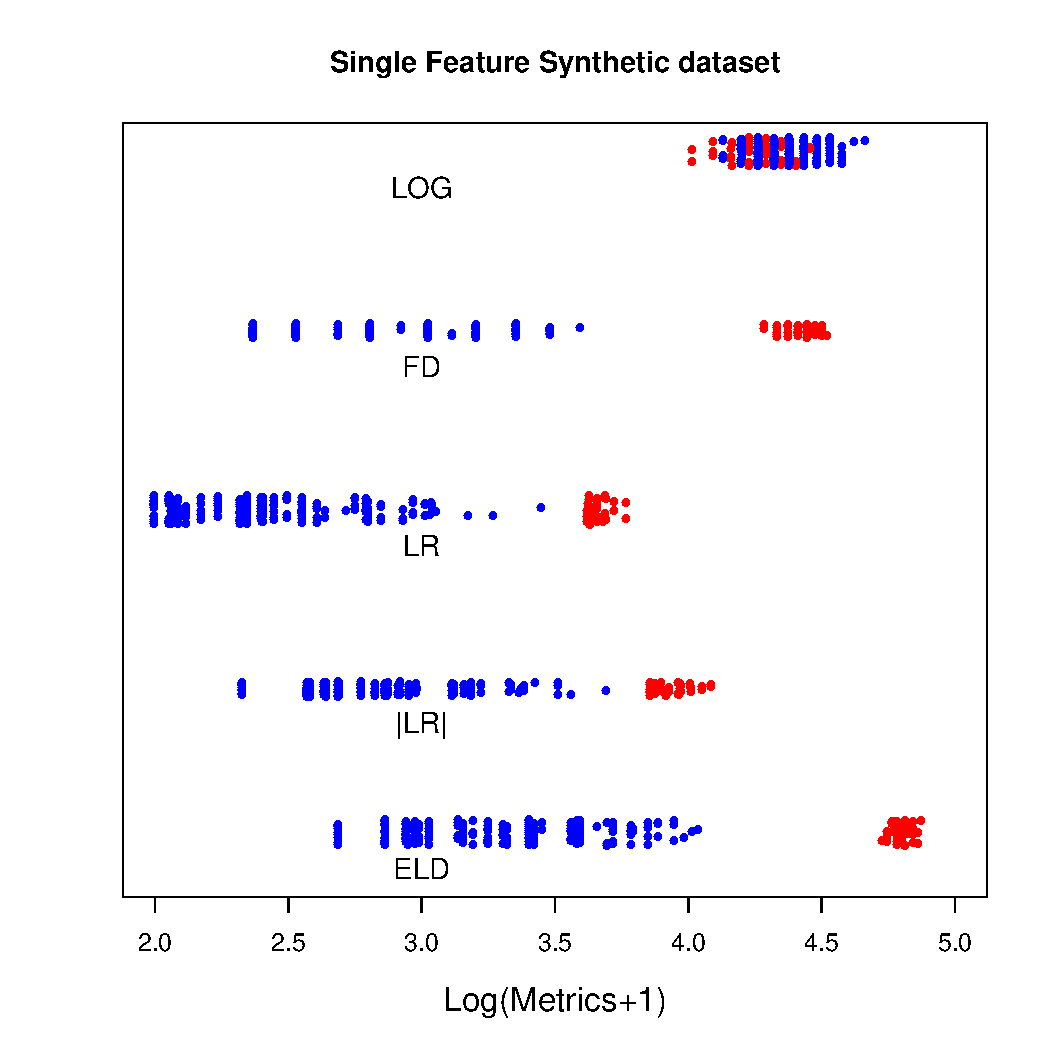
\includegraphics[width=0.48\textwidth]{DistributionPlots/featureSep.pdf}}
							\subfigure[Distribution of different outlier scores in Synthetic Dataset- Low correlation]{\label{fig:LowCor}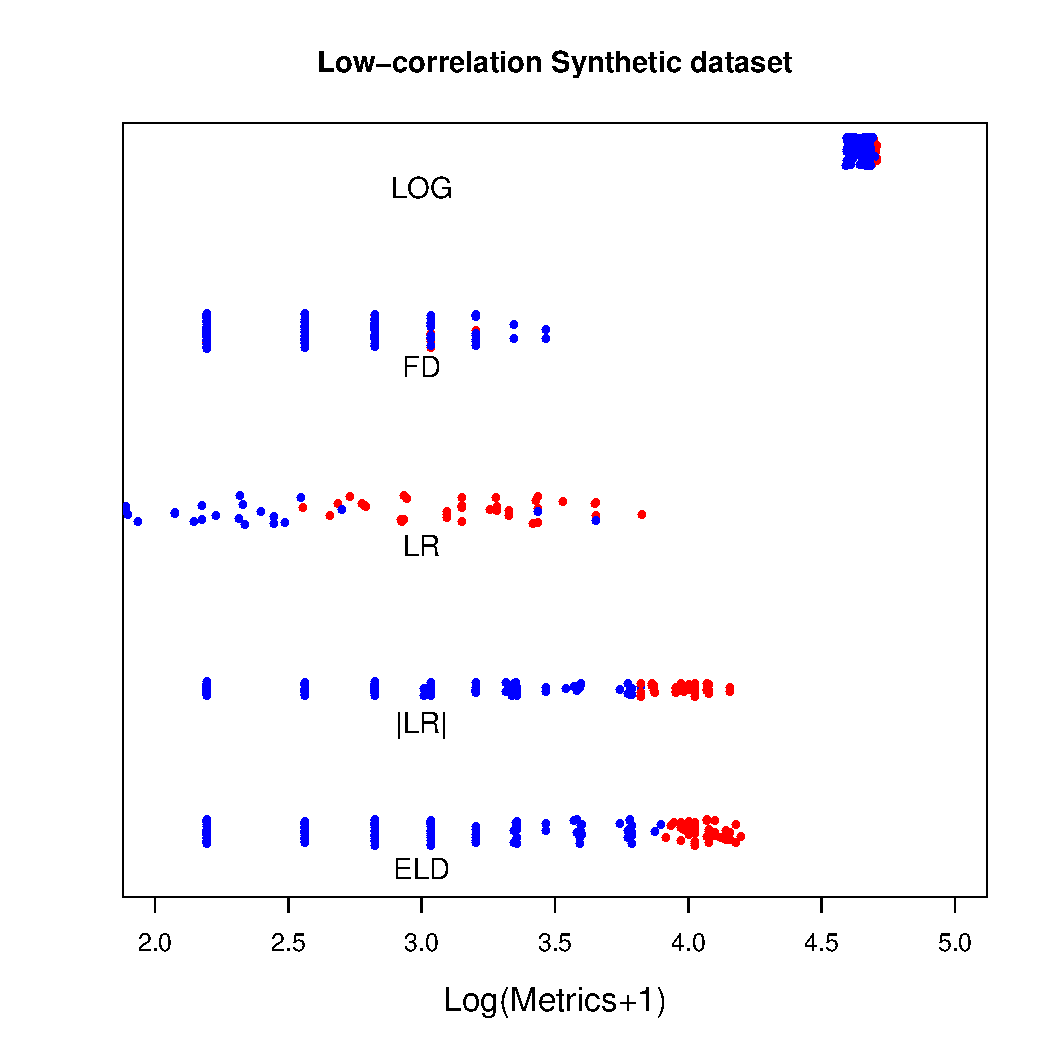
\includegraphics[width=0.5\textwidth]{DistributionPlots/low-Sep}}
							\subfigure[Distribution of different outlier scores in Synthetic Dataset- High correlation]{\label{fig:HighCor}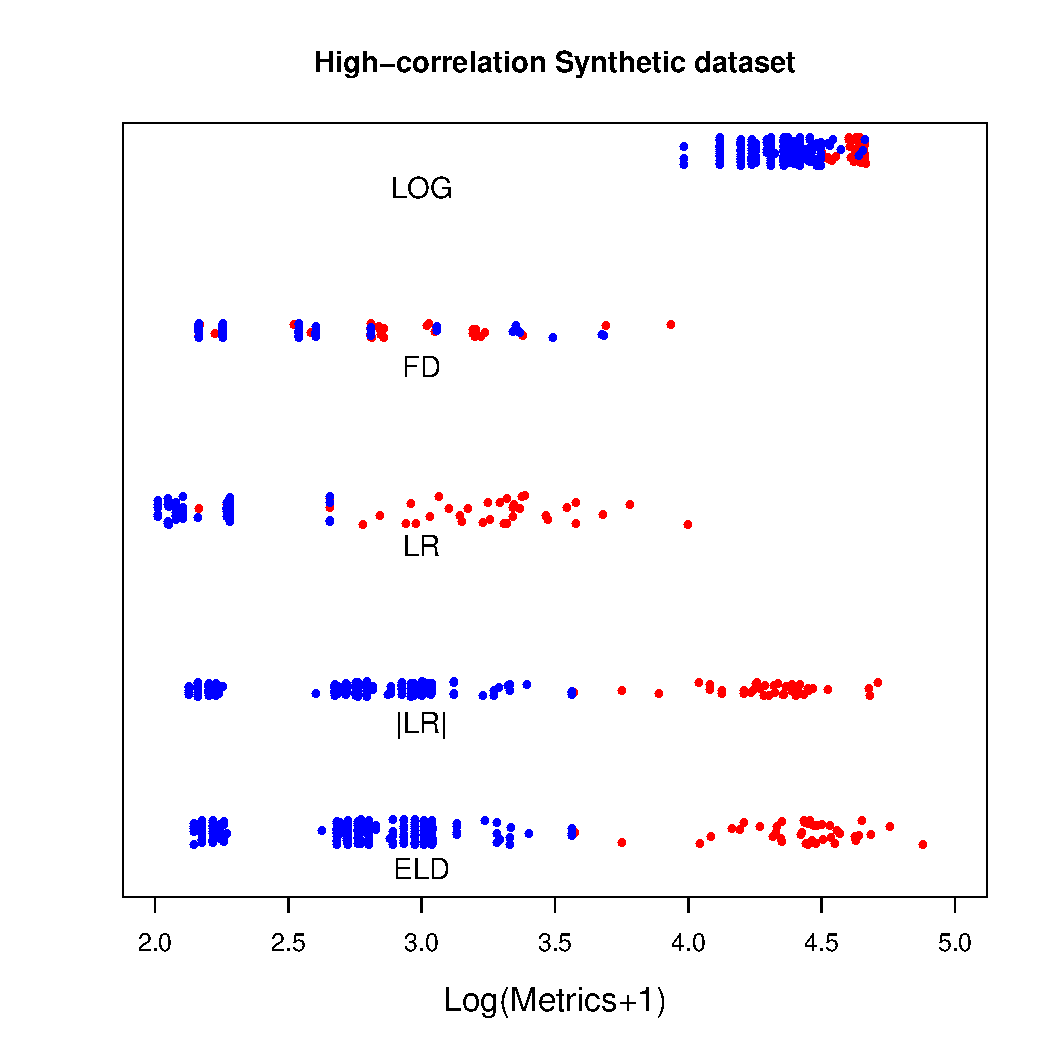
\includegraphics[width=0.5\textwidth]{DistributionPlots/high-Sep}}
							\caption{Visualizing likelihood-based outlier metrics on our three synthetic datasets. We employed log scale to to show the score values of different range in a single plot. To avoid the negative numbers for the values between 0 and 1, we used metric+1.  The figure is best viewed in colors. Score values are shown on the $x$-axis; higher values should indicate more anomalous players. For each dataset and each metric, we provide a 1D scatterplot of the 280 synthetic player scores. In the scatterplot, blue dots represent normal players, and red dots represent anomalous players. }\label{fig:1DPlots}
						\end{figure}
						
						
		
		
			
		%section{Examples} \label{sec:divergence-examples} 
		
		
		
		
%\begin{table}[hbpt]
%	\caption{Example Computation of different outlier scores.
%		% for the examples.
%		% of Figure~\ref{fig:synthetic-bns}(a),(b). 
%	} 
%	\label{table:example}
%	
%	%\captionsetup[table]{skip=10pt}
%	
%	\centering
%	\resizebox{1\textwidth}{!}{
%		\begin{tabular}{|c|p{3cm}|p{6cm}|l|}
%			\hline
%				Score&$F1=1$ Computation&$F2|F1=1$ Computation&Result\\ \hline
%				$\lr$&$1/2\ln(0.5/0.5)=0$&$0.25 \ln(0.5/0.9)+ 0.25 \ln(0.5/0.1)$&0.36\\ \hline
%				%$ELD$&$1/2|\ln(0.5/0.5)=0|$&$0.5 \cdot 0.9|\ln(0.9/0.5)|+0.5 \cdot 0.1|\ln(0.1/0.5)|$&0.50\\ \hline
%				$|\lr|$&$0$ (no parents) &$0.25 |\ln(0.5/0.5)-\ln(0.9/0.5)|+ 0.25 |\ln(0.5/0.5)-\ln(0.1/0.5)| $&0.79\\ \hline
%				$\fd$&$|\ln(0.5/0.5)|=0$&$0.5|\ln(0.5/0.5)| + 0.5|\ln(0.5/0.5)|$&0\\ \hline
%				$\mid$&$0+0$&$0.79+0$&0.79\\ \hline
%	%		\\ \hline
%		\end{tabular}}
%		%\centering
%		\resizebox{0.7\textwidth}{!}{
%			\begin{tabular}{p{8cm}}
%				Table V(a): High Correlation Case, Figure~\ref{fig:synthetic-bns}(a).
%				%: The scores for the object and class BNs of Figure~\ref{fig:synthetic-bns}(a).
%				
%			\end{tabular}}
%			
%			%
%			\centering
%			\resizebox{1\textwidth}{!}{
%				\begin{tabular}{|l|p{3cm}|p{6cm}|l|}
%					\hline
%					Score&$F1=1$ Computation&$F2|F1=1$ Computation&Result\\ \hline
%					$\lr$&$1/2\ln(0.5/0.5)=0$&$0.5 \cdot 0.9 \ln(0.9/0.5)+ 0.5 \cdot 0.1 \ln(0.1/0.5)$&0.26\\ \hline
%					%$ELD$&$1/2|\ln(0.5/0.5)=0|$&$0.5 \cdot 0.9|\ln(0.9/0.5)|+0.5 \cdot 0.1|\ln(0.1/0.5)|$&0.50\\ \hline
%					$|\lr|$&$0$ (no parents) &$0.5 \cdot 0.9 |\ln(0.9/0.5)-\ln(0.5/0.5)|+ 0.5 \cdot 0.1 |\ln(0.1/0.5)-\ln(0.5/0.5)| $&0.50\\ \hline
%					$\fd$&$|\ln(0.5/0.5)|=0$&$1/2|\ln(0.5/0.5)| + 1/2|\ln(0.5/0.5)|$&0\\ \hline
%					$\mid$&$0+0$&$0.5+0$&0.5\\ \hline
%				\end{tabular}}
%				\resizebox{0.7\textwidth}{!}{
%					\begin{tabular}{p{8cm}}
%						Table V(b): Low Correlation Case. Figure~\ref{fig:synthetic-bns}(b).
%						%The scores for the object and class BNs of Figure~\ref{fig:synthetic-bns}(b). 
%						
%					\end{tabular}}
%				\end{table}
%				

					
					
													
			\section{Experimental Design}
			%Details about our systems and algorithms that we use from previous work may be found in Section~\ref{sec:details}.  
			All the experiments were performed on a 64-bit Centos machine with 4GB RAM and an Intel Core i5-480 M processor. The likelihood-based outlier scores were computed with SQL queries using JDBC, JRE 1.7.0. and MySQL Server version 5.5.34.
			We describe the datasets used in our experiments.
			
%			\subsection{Synthetic Datasets}
%			
%			We generated three synthetic datasets with normal and outlier players using the distributions represented in the three Bayesian networks of Figure~\ref{fig:synthetic-bns}. 
%			%The features $F_{1}$ and $F_{2}$ represent two features of players. 
%			Each player participates in 38 matches, similar to the real-world data. The main goal of designing synthetic experiments is to test the methods on  easy to detect outliers. Each match assigns a value to each feature $F_i, i =  1,2$ for each player. 
%			\begin{description}
%				\item\textbf{High Correlation} See Figure~\ref{fig:synthetic-bns}(a).
%				\item\textbf{Low Correlation} See Figure~\ref{fig:synthetic-bns}(b).
%				\item\textbf{Single features} See Figure~\ref{fig:synthetic-bns}(c).
%			\end{description}
%			
%			
%			
%			
%			
%			%These datasets are designed so that outliers and normal objects are easy to distinguish, and so that it is easy to trace the behavior of an outlier score.
%			
%			%\begin{description}
%			%\item[High Correlation]  See Figure~\ref{fig:synthetic-bns}(a).
%			%\item[Low Correlation]  See Figure~\ref{fig:synthetic-bns}(b).
%			%\item[Single attributes] See Figure~\ref{fig:synthetic-bns}(c).
%			%\end{description}
%			%
%			We used the $\it{mlbench}$ package in $\it{R}$ to generate synthetic features in matches, following these distributions for 240 normal players and 40 outliers. We followed the real-world Opta data in terms of number of normal and outlier individuals. The scores are used to rank all 280 players. 
%			\subsection{Real-World Datasets} \label{sec:real-world-data}
%			Data tables are prepared from Opta data~\cite{opta-original} and IMDb~\cite{IMDb-original}. Our datasets and code are available on-line~\cite{bib:jbnsite}.
%			\paragraph{Soccer Data} 
%			The Opta data were released by Manchester City. 
%			It lists box scores, that is, counts of all the ball actions within each game by each player, for the 2011-2012 season. 
%			%The data consists of information about the actions of a single player in a given match 
%			%from 2011 to 2012. 
%			%Number of goals, passes, fouls, tackles, saves and blocks and also position 
%			%assigned to a player in a match are examples of the information associated with each player. [list]
%			%Information about the teams in a season, such as number of home wins, draws or away wins can be extracted by massaging the data. 
%			%[The information can be visualized as a heterogeneous network that links players to teams, and teams to matches. ]
%			For each player in a match, our data set contains eleven player features.
%			% like $\it{TimePlayed}(\P,\M)$.
%			For each team in a match, there are five features computed as player feature aggregates, as well as the team formation and the result (win, tie, loss). 
%			There are two relationships, $\it{Appears\_Player}(\P,\M)$, $\it{Appears\_Team}(\T,\M)$. 
%			%We store the data in a relational database, with a table for each base population and a table for each relationship.
%			
%			\paragraph{IMDB Data} 
%			The Internet Movie Database (IMDB) is an on-line database of information related to films, television programs, and video games.
%			The IMDB website offers a dataset containing information on cast, crew, titles, technical details and biographies into a set of compressed text files. 
%			We preprocessed the data like \cite{Peralta2007} to obtain a database with seven tables: one for each population and one for the three relationships $\it{Rated}(\user,\movie)$, $\it{Directs}(\director,\movie)$, and $\it{ActsIn}(\actor,\movie)$.
%			
%			%				Table~\ref{table:Features} lists relationships and the number of features. 
%			%				\begin{table}[htbp]
%			%							\caption{Relationships and Example Features in Real-World Datasets.
%			%								%For relationships please see text.
%			%								\label{table:Features}}
%			%					\centering
%			%					\resizebox{0.3\textwidth}{!}{
%			%						\begin{tabular}{|l|c|l|}
%			%							\hline
%			%							Path/Object Type & \#Attributes&Example\\ \hline
%			%							\begin{tabular}{c}Player-Team-Match \end{tabular} & 11&ShotEff \\ \hline
%			%							\begin{tabular}{c}Team-Match \end{tabular} & 7&TeamFormation \\ \hline\hline
%			%							Actor & 2&Quality \\ \hline
%			%							Director & 2&AvgRevenue\\ \hline
%			%							Movie&5&Genre\\ \hline
%			%							User& 2&Occupation\\ \hline
%			%							User-Movie & 1&Rating \\\hline
%			%							Actor-Movie & 1&Cast\_Position\\\hline
%			%						\end{tabular}}
%			%				
%			%					\end{table}
%			%\footnote{Commented table of relationships and features}
%			%					\begin{LaTeXdescription}
%			%						\item[Soccer Data]
%			%						The Opta data were released by Manchester City. 
%			%						It lists all the ball actions within each game by each player, for the 2011-2012 season.
%			%						\item[IMDb Data]
%			%						The Internet Movie Database (IMDb) is an online database of information related to films, television programs, and video games.
%			%						The IMDb website offers a dataset containing information on cast, crew, titles, technical details and biographies in a set of compressed text files \cite{Peralta2007}.
%			%					\end{LaTeXdescription}
%			
%			%\subsection{Outlier and Contrast Classes.}
%			
%			In real-world data, there is no ground truth about which objects are outliers. To address this issue, we employ a one-class design: we learn a model for the class distribution, with data from that class only. Then we rank all individuals from the normal class together with all objects from a contrast class treated as outliers, to test whether an outlier score recognizes objects from the contrast class as outliers.
%			%		distinguishes objects from the normal class from objects in the contrast class. 
%			Table~\ref{MetricComputation} shows the normal and contrast classes for three different datasets.  In-class outliers are possible, e.g. unusual strikers are still members of the striker class. Our case studies describe a few in-class outliers. In the soccer data, we considered only individuals who played more than 5 matches out of a maximum 38. 
%						
%						\begin{table}
%							\caption{Outlier/normal Objects in Real-World Datasets. }
%							\label{MetricComputation}
%							\centering
%							\resizebox{0.4\textwidth}{!}{
%								\begin{tabular}{|c|c|c|c|}
%									\hline
%									Normal&\#Normal&Outlier&\#Outlier\\\hline
%									Striker & 153 & Goalie&22\\ \hline
%									Midfielder & 155 & Striker&74\\ \hline
%									Drama & 197 & Comedy&47\\ \hline
%									%Synthetic&40&280\\ \hline
%								\end{tabular}}
%								
%							\end{table}
%							
%							
%							\begin{figure*}[htbp]
%								\centering
%								\resizebox{1\textwidth}{!}{
%									\includegraphics%[width=0.3\textwidth] 
%									{figures/figure1kddCropped.pdf}
%								}
%								\caption{Illustrative Bayesian networks. The networks are not learned from data, but hand-constructed to be plausible for the soccer domain. (a) High Correlation: Normal individuals exhibit a strong association between their features, outliers no association. Both normals and outliers have a close to uniform distribution over single features.
%									% The outlier distribution misses a correlation that is present in the normal population. The single feature distributions are uniform in both distributions. 
%									(b) Low Correlation: Normal individuals exhibit no association between their features, outliers have a strong association. Both normals and outliers have a close to uniform distribution over single features.
%									% The outlier object exhibits a correlation that is not present in the normal population. The single attribute distributions are uniform in both distributions.
%									(c) Single Attributes: Both normal and outlier individuals exhibit a strong association between their features. In normals, 90\% of the time, feature 1 has value 0. For outliers, feature 1 has value 0 only 10\% of the time. 
%									%Correlations are the same, but the single feature distributions are not.
%									\label{fig:synthetic-bns}}
%							\end{figure*}
%							
%							\begin{figure}[t]
%								\centering
%								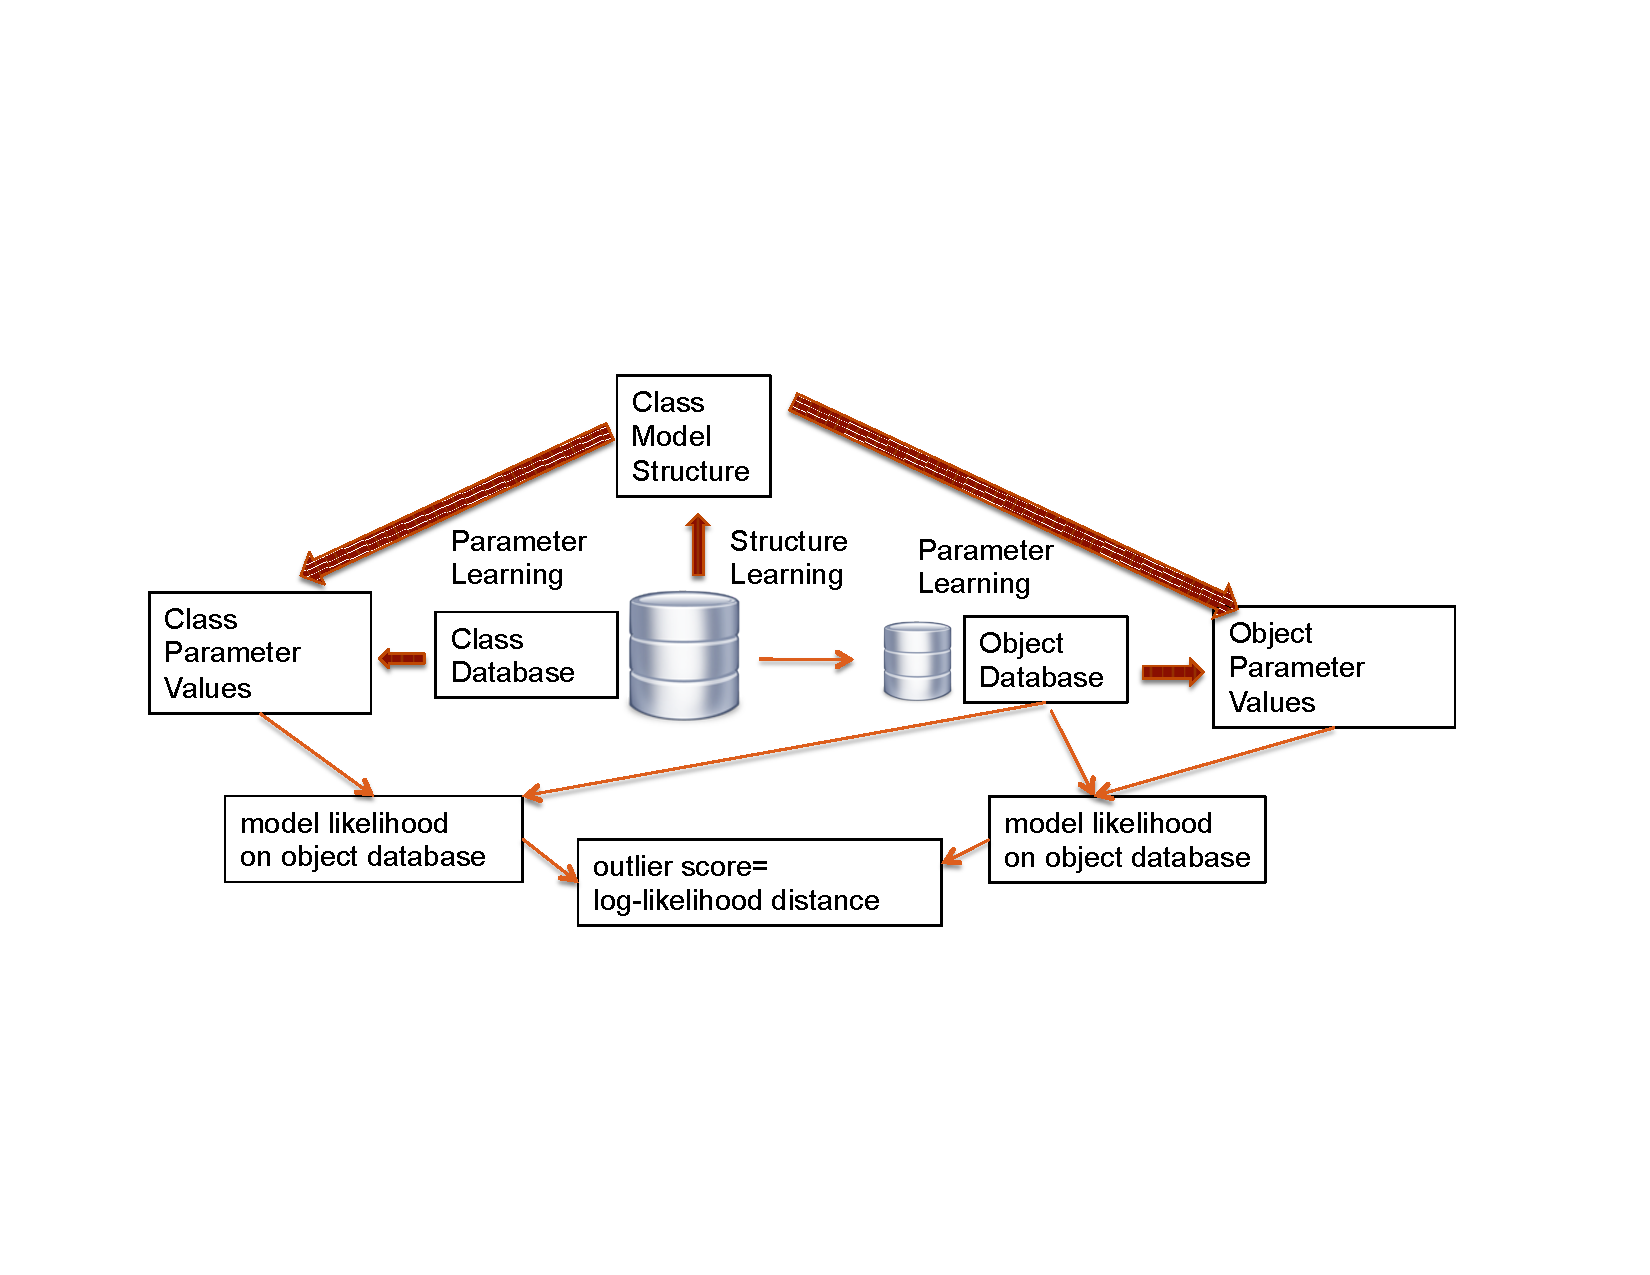
\includegraphics[width=1\textwidth]{figures/flow.pdf}
%								\caption{Computation of outlier score. 
%									\label{fig:flow}}
%							\end{figure}
							
								\subsection{Methods Compared}
								\label{sec:methods}
								We compare two types of approaches, and within each approach several outlier detection methods. The first approach evaluates the likelihood-based outlier scores described in section~\ref{sec:metrics}. For relational Bayesian network structure learning we utilize the previous learn-and-join algorithm (LAJ) that was introduced in chapter~\ref{chap:three}.
%								which is
							%	a state-of-the-art BN structure learning method for relational data \cite{Schulte2012}. The LAJ algorithm employs an iterative deepening strategy, which can be described as as search through a lattice of table joins. For each table join, different BNs are learned and the learned edges are propagated from smaller to larger table joins. 	For a full description, complexity analysis, and learning time measurements, please see \cite{Schulte2012}. 	We used the implementation of the LAJ algorithm due to its creators \cite{bib:jbnsite}. 
								
								%						probabilistic scores applied directly to the  data structured as an object tree. 
								
								The second approach is to compare the loglikelihood metric with some of the standards matrix-based outlier analysis methods. One way to convert relational data to a single data matrix is to first ``flattens" the structured data into a matrix of feature vectors, then applies standard matrix-based outlier detection methods. We refer to such methods as \textbf{propositional-based}
								%Flattening the object data allows applying the rich set of matrix-based outlier detection methods ``as is" 
								(cf. Figures~\ref{fig:novelty}). For example, this was the approach taken by Breunig {\em et al.} for identifying anomalous players in sports data \cite{Breunig2000}.
								However, as discussed in chapter~\ref{chap:four}, aggregation 
								tends to lose information about correlations and MLN propositionalization is a better candidate for this conversion. Therefore, instead of aggregating over features, we used features generated by MLN-TF. In chapter~\ref{chap:four} we showed that in most datasets, MLN-TF produce better quality features compare to the other propositionalization methods.
								% Following their paper, for each continuous feature in the object data, we use the average over its values, and for each discrete feature, we use the occurrence count of each feature value in the object data.
								%\cite{DavidJensen2002}. 
							%	Our experiments address the empirical question of whether this loss of information affects outlier detection. 
								%The advantage to the aggregation approach is that after aggregating to preprocess the data, any matrix-based outlier detection method can be applied; see Figure~\ref{fig:flow}. 
								We evaluated three standard propositional-based outlier detection methods: Density-based $\lof$~\cite{Breunig2000}, distance-based $\knn$~\cite{Ramaswamy2000} and subspace analysis $\outrank$~\cite{Muller2012}.
								%\footnote{commented descriptions of these methods }. 
								These represent common, fundamental  approaches for propositional data. 
								%	Subspace analysis is especially relevant to our study because 
%								Like $\mid$, subspace analysis is sensitive to correlations among features. 
%								% Our experiments applied $\outrank$ with two subspace clustering models, \textit{PRO-CLUS} \cite{Muller2012} and \textit{DISH} \cite{Kriegel2007}.  
%								We used the available implementation of all three data matrix methods from the state of the art data mining software \textit{ELKI} \cite{Elke2013}. We used \textit{PRO-CLUS} as the clustering function for $\outrank$, recommended by~\cite{Muller2012}.
%								
								
%								\begin{description}
%									\item[$\lof$] is a standard density-based method~\cite{Breunig2000}.
%									It quantify the outlier-ness of the data points relative to regions of different densities. Therefore, the score is defined based on local density instead of the nearest neighbor distance. In simple words, 
%									$\lof$ compares the density of area around an object to the densities of the areas of the surrounding objects. 
%									However, $\lof$ defines density as the inverse of the average of the smoothed reachability distances in a neighborhood and this definition is not the precise definition of density in terms of number of data points within a specific region. $\lof$ is only sensitive to the density of the area and  ignore the orientation and the shape of the area. Figure~\ref{fig:lof} shows the basic idea of $\lof$.
%									\item[$\knn$] is a well-known distanced-based outlier ranking method that assigns a score to each data point on the basis of distance of the point from its $k^{th}$ nearest neighbor ($D^k$) and  declare the top $n$ points as outliers~\cite{Ramaswamy2000}. 
%									They introduce a {\em partition-based} algorithm to set a upper bound and lower bound on $D^k$ to identify the partitions that cannot contain the top $n$ outliers and prune them in order to limit the search space. % \textbf{Sarah:more precise please}
%									\item[$\outrank$] employs subspace analysis to measure the degree of outlierness. It compares clusters in different subspace to derive an outlier score for each object. This method has been explain in more details in Chapter~\ref{chap:two}.
%									
%									
%									
%											\begin{figure*}[htbp]
%												\centering
%												\resizebox{0.45\textwidth}{!}{
%													\includegraphics%[width=0.3\textwidth] 
%													{figures/lof-pic.pdf}
%												}
%												\caption{ Point A has a high LOF score because its density is lower than its neighbours densities. Dotted circles show the distance to each point's third nearest neighbour.
%													%Correlations are the same, but the single feature distributions are not.
%													\label{fig:lof}}
%											\end{figure*}
%									\end{description}
%								
%								Density and distance based methods are two fundamental approaches to outlier detection represented in our study by $\lof$ and $\knn$. Subspace analysis is a popular approach too, and relevant to our study because $\mid$ is sensitive to correlations among attributes as well. The $\outrank$ research of~\cite{Muller2012} suggests that \textit{PRO-CLUS} is the best clustering function for their approach. Our experiments applied $\outrank$ with two subspace clustering models, \textit{PRO-CLUS} \cite{Muller2012} and \textit{DISH} \cite{Kriegel2007}.  
%								We used the available implementation of all three data matrix methods from the state of the art data mining software \textit{ELKI} \cite{Elke2013}. 
%								
								
										\section{Empirical Results}
										
										We present results regarding computational feasibility, 
										%$\auc$ 
										predictive performance, and case studies.
										
										\subsubsection{Computational Cost of the $\mid$ Score.}
										%						
										%						Table~\ref{table:Number of Parameters} shows that the Bayesian network representation provides a highly compact summary of the target class distribution: the number of probabilities that need to be evaluated for computing the probabilistic scores decreases by a factor of 
										%						%\textbf{Sarah:fix dash}
										%						$10^{4}$\--$10^{5}$ depending on the dataset. 
										%						
										Table~\ref{table:LearningTime} shows that the computation of the $\mid$ value for a given target object is feasible. On average, it takes a quarter of a minute for each soccer player, and one minute for each movie. This includes the time for parameter learning from the object database.
										Learning the class model BN takes longer, but needs to be done only once for the entire object class. 
										{\em The BN model 
											%						is crucial for computational feasibility because it 
											provides a crucial %compact 
											low-dimensional representation of the 
											%joint 
											distribution information in the data.} Table~\ref{table:Number of Parameters} compares the number of terms required to compute the $\mid$ score in the BN representation to the number of terms in an unfactored representation with one parameter for each joint probability.
										
										\begin{table}[htbp]
												\centering
											\begin{subtable}
												%\caption{Time for computing the $\mid$ metric. This includes the time for Bayes Net structure learning.\label{table:LearningTime}}
												\centering
												\caption{Time (min) for computing the $\mid$ score. 
													%This includes the time for Bayes Net structure learning.
													\label{table:LearningTime}}
												\resizebox{0.8\textwidth}{!}{
													\begin{tabular}{|c|l|l|} \hline
														Dataset& Class Model
														%    \begin{tabular}{c} Class \\Terms (min)\end{tabular}   & 
														%    \begin{tabular}{c} Object \\Terms (min)\end{tabular}   
														& Average per Object  \\ \hline
														Strikers vs. Goalies&4.14&0.25\\ \hline
														Midfielder vs. Goalies &4.02&0.25 \\ \hline
														Drama vs. Comedy &8.30&1.00\\ \hline
													\end{tabular} 
												}
												
											\end{subtable}
											
											\begin{subtable}
												%\caption{The Bayesian network representation helps to decrease the number of terms that represent the class and object distributions. 
												%For relationships please see text.
												%\label{table:Number of Parameters}}
												\centering
												\caption{The Bayesian network representation decreases the number of terms required for computing the $\mid$ score.
													%that represent the class and object distributions.
													\label{table:Number of Parameters}}
												\resizebox{0.8\textwidth}{!}{
													\begin{tabular}{|c|l|l|}
														\hline
														Dataset & \begin{tabular}{c} \#Terms \\Using BN\end{tabular}  & \begin{tabular}{c} \#Terms \\ without Using BN
														\end{tabular}\\ \hline
														Strikers vs. Goalies & 1,430&114,633,792\\ \hline
														Midfielders vs. Goalies & 1,376&43,670,016\\ \hline
														Drama vs. Comedy & 50,802&215,040,000\\ \hline
													\end{tabular}
												}
												
											\end{subtable}
											
										\end{table}
												\subsubsection{Detection Accuracy} \label{sec:detection}
												 Our experiments provide empirical evidence that in practice $\mid$ generally works better than other scores for object outlier detection.
										
												 %We evaluate the performance of $\mid$ compared to other outlier different metrics.
												 Our performance score for outlier rankings is the area under curve ($\auc$) of the well-established receiver operating characteristic $\roc$ curve.
												 ~\cite{Fawcett2006}. 
												 This has been widely used to measure the performance of outlier ranking methods~\cite{Cansado2008, Muller2012}. The relationship between false positive rate (1- Specificity) and true positive rate (Sensitivity) is captured by the $\roc$ curve. Ideally, the best performance is achieved when we have the highest sensitivity and the highest specificity. 
												 %The area under the \textit{ROC} curve shows the overall performance and it is a measure to compare the curves numerically. 
												 The maximum values for $\auc$ is, 1.0 indicating a perfect ranking with 100\% sensitivity and 100\% specificity. In order to compute the $\auc$ value, we used the \textit{R} package \textit{ROCR}~\cite{RROCR2012}. Given a set of outlier scores, one for each object, this package returns an $\auc$ value. 
												 \begin{table}
												 \begin{subtable}
												 	
												 	\centering
												 	\resizebox{0.8\textwidth}{!}{
												 		\begin{tabular}{|l|l|l|l|l|l|}
												 			\hline
												 			Dataset & \mid&$|\lr|$ &\lr &\fd&\loglikelihood\\ \hline
												 			
												 			High Correlation & \textbf{1.00}&0.99&0.97&0.88&0.98 \\ \hline
												 			Low Correlation & \textbf{1.00}&0.99&0.98&0.35&0.81 \\ \hline
												 			Single Feature & \textbf{1.00}&\textbf{1.00}&\textbf{1.00}&\textbf{1.00}&0.79 \\ \hline
												 			Strikers vs. Goalies & \textbf{0.89} &0.77&0.65&0.71& 0.61\\ \hline
												 			Midfielders vs. Strikers &\textbf{0.66}&{0.62} &0.55 &0.59&0.54 \\ \hline
												 			Drama vs. Comedy & \textbf{0.70} &0.68&0.66&0.64&0.66 \\ \hline
												 		\end{tabular}}
												 		\caption{AUC of $\mid$ vs. other probabilistic scores. 
												 			%For relationships please see text.
												 			\label{table:Metric Comparison}}
												 	\end{subtable}
												 	
%												 	\begin{subtable}
%												 		
%												 		\centering
%												 		\resizebox{1\textwidth}{!}{
%												 			\begin{tabular}{|c|c|c|c|c|c|}
%												 				\hline
%												 				Dataset & $\mid$ &$\lof$&\begin{tabular}{c}$\outrank$\\(ProClus)\end{tabular}&\begin{tabular}{c}$\outrank$\\(DISH)\end{tabular}&\begin{tabular}{c}\it{KNN}\\\it{Outlier}\end{tabular}\\ \hline
%												 				
%												 				High Correlation & \textbf{1.00}&0.87&0.73&0.95&0.92 \\ \hline
%												 				Low  Correlation & \textbf{1.00}&0.53&0.33&0.32&0.45 \\ \hline
%												 				Single Feature & \textbf{1.00}&0.58&\textbf{1.00}&0.96&0.95\\ \hline
%												 				Strikers vs. Goalies & \textbf{0.89} &0.68&0.89&0.53&0.75 \\ \hline
%												 				Midfielders vs. Strikers &\textbf{0.66} &0.53 &0.54&0.49&0.55 \\ \hline
%												 				Drama vs. Comedy & \textbf{0.70} &0.53&0.56&0.42&0.61 \\ \hline
%												 			\end{tabular}}
%												 			\caption{AUC of $\mid$ vs. aggregation-based outlier detection methods. 
%												 				%For relationships please see text.
%												 				\label{table:Method Comparison} 
%												 			}
%												 		\end{subtable}
												 		
												 		
												 		 	\begin{subtable}
												 						 		
													 		\centering
						 							 		\resizebox{1\textwidth}{!}{								 							 			\begin{tabular}{|c|c|c|c|c|}
												 							\hline
												 			 				Dataset & $\mid$ &$\lof$&OutRank&\begin{tabular}{c}\it{KNN}\\\it{Outlier}\end{tabular}\\ \hline
												 							 				
												 		 				High Correlation & \textbf{1.00}&0.68&0.99&0.97 \\ \hline
													 				Low  Correlation & \textbf{1.00}&0.58&0.83&0.97 \\ \hline
						 							 				Single Feature & \textbf{1.00}&0.63&0.88&0.86\\ \hline										 							 				Strikers vs. Goalies & \textbf{0.89} &0.61&0.60&0.63 \\ \hline
												 					Midfielders vs. Strikers  &0.66 &\textbf{0.76} &0.71&0.58 \\ \hline
													 				Drama vs. Comedy & \textbf{0.70} &0.51&0.68&0.68\\ \hline
							 							 			\end{tabular}}
							 							 			\caption{AUC of $\mid$ vs. propositional-based outlier detection methods. The single table used as input for $\outrank$, $\lof$ and  $\knn$ was generated using the  MLN-TF, a propositionalization approach introduced in chapter~\ref{chap:three}.								 							 			 	%For relationships please see text.
												 					\label{table:proposMethod Comparison} 
												 							 			}
												 							 		\end{subtable}
												 	\end{table}
%												 We follow the evaluation design of~\cite{Gao2010} and 
%												make each baseline methods detect the same percentage of  objects as outliers:
%												% as that of the ground-truths. To achieve this, we 
%												Sort the outlier scores obtained by the three baseline methods in descending order, and take the top $r$ percent as outliers. Then we use \textbf{precision}, a.k.a. \textbf{true positive rate} as the evaluation metric which is the percentage of correct ones in the set of outliers identified by the algorithm. As in~\cite{Gao2010}, we set the percentages of outlier to be 1\% and 5\%. In the one-class design, precision measures how many members of the outlier class were correctly recognized. We also report some AUC measurements \cite{aggarwal2013}, which aggregate precision values at different percentage cutoffs.\footnote{Our $\mid$ score performs the best also with other metrics such as recall, to a similar degree; we omit the details due to space constraints.} %\textbf{Sarah: I'd love to have the plots of all points here.}
%												
%												
%												\paragraph{Likelihood-Based Methods} 
%												
%												
%												Table~\ref{table:Method Comparison} shows the $\auc$ values for each probabilistic ranking. Our $\mid$ score achieves the top score on each dataset. On the synthetic data, $\mid$ and $|\lr|$ are the only scores with 100\% precision at 1\% and 5\%. This confirms the value of using distances rather than differences. 
%												%						However, the AUC score shows that $\mid$ retains perfect detection with different percentage cutoffs, but $|\lr|$ ranks some normal objects higher than actual outliers. 
%												While it ought to be easy to distinguish the outliers, Table~\ref{table:Metric Comparison} shows that {\em $\mid$  is the only score that achieves perfect detection}, that is AUC = 1.0.
%												
%													\begin{table}
%														\caption{Precision of outlier scores in different datasets.
%															\label{table:Method Comparison}}
%														\resizebox{1\textwidth}{!}{	
%															\begin{tabular}{|l|c|c|c|c|c|c|c|c|c|}\hline
%																Dataset& percentage&\multicolumn{5}{|c|}{Model-based models }&\multicolumn{3}{|c|}{Aggregation-based models}\\
%																\hline
%																& &\mid&$|\lr|$&\lr&\fd&\loglikelihood&\lof&$\outrank$	&\knn\\
%																\hline
%																\multirow{2}{*}{High-Correlation}& 1\%& \textbf{1.00}& \textbf{1.00}& 0.73& 0.47& 0.91& 0.11& 0.53& 0.48\\
%																&5\%&\textbf{1.00}&\textbf{1.00}&0.85&0.65&0.95&0.22&0.50&0.65\\
%																\hline																				    	 \multirow{2}{*}{Low-Correlation}& 1\%& \textbf{1.00}& \textbf{1.00}& 0.87& 0.14& 0.93& 0.10& 0.00& 0.06\\
%																&5\%&\textbf{1.00}&\textbf{1.00}&0.90&0.25&0.95&0.25&0.10&0.14\\
%																\hline
%																\multirow{2}{*}{Single-Feature}& 1\%& \textbf{1.00}& \textbf{1.00}& 0.39& 0.53& 0.81& 0.46& \textbf{1.00}& 0.51\\
%																&5\%&\textbf{1.00}&\textbf{1.00}&0.55&0.62&0.92&0.55&\textbf{1.00}&0.54\\
%																\hline    
%																\multirow{2}{*}{Striker-Goalie}& 5\%& \textbf{0.57}& 0.27& 0.22& 0.51& 0.36& 0.19& 0.47& 0.42\\
%																&15\%&\textbf{0.63}&0.36&0.31&0.58&0.40&0.32&0.50&0.52\\
%																\hline    
%																\multirow{2}{*}{Midfielder-Striker}& 1\%&\textbf{ 0.49}& 0.42& 0.25& 0.41& 0.46& 0.29& 0.44& 0.16\\
%																&5\%&\textbf{0.52}&0.48&0.39&0.44&0.50&0.38&0.48&0.35\\
%																\hline  																				\multirow{2}{*}{Drama-Comedy}&1\%& \textbf{0.44}& 0.38& 0.39& 0.15& 0.22& 0.29& 0.07& 0.014\\
%																&5\%&\textbf{0.47}&0.45&0.44&0.40&0.28&0.36&0.17&0.20\\
%																\hline     
%																
%															\end{tabular}	}		
%															
%														\end{table}
%																\begin{table}
%																	\centering
%																	\caption{\textit{AUC} of $\mid$ vs. $|LR|$. 
%																		%For relationships please see text.
%																		\label{table:Metric Comparison}}
%																	\resizebox{1\textwidth}{!}{
%																		\begin{tabular}{|l|l|l|l|l|l|l|}\hline
%																			Score & High-Cor. &Low-Cor.&Single-F.&Striker&Midfielder&Drama\\ \hline
%																			\mid&1.00&1.00&1.00&0.89&0.66&0.70\\\hline
%																			$|\lr|$&0.95&0.95&0.89&0.61&0.64&0.65\\\hline
%																			%	Synthetic Data-High Correlation & \textbf{1.00}&0.95 \\ \hline
%																			%	Synthetic Data-Low Correlation & \textbf{1.00}&0.95 \\ \hline
%																			%	Synthetic Data-Single Feature & \textbf{1.00}&0.89 \\ \hline
%																			%									Real Data-Strikers vs. Goalies & \textbf{0.89} &0.61\\ \hline
%																			%									Real Data-Midfielders vs. Strikers &\textbf{0.66} &0.64 \\ \hline
%																			%									Real Data-Drama vs. Comedy & \textbf{0.70} &0.65 \\ \hline
%																		\end{tabular}}
%																		
%																	\end{table}
\paragraph{Probabilistic Structured methods:}
Table~\ref{table:Metric Comparison} shows the $\auc$ values for each probabilistic ranking. On the synthetic data, it ought to be easy to distinguish the outliers. Single feature is the easiest dataset and most metrics except $\log$ are successful in perfectly detecting outliers.  However, $\mid$ is the only score that achieves the perfect detection across all three synthetic datasets. 
																	\paragraph{Propositionalization-Based Methods vs. \mid} 
																	Table~\ref{table:proposMethod Comparison} shows the precision values for propositional-based methods compared to $\mid$. {\em Our $\mid$ score outperforms all Propositional-based methods on all datasets}, except for one real-world dataset that $\lof$ outperform $\mid$ and that is with the help of conjunctive features generated by the  propositionalization method introduced in chapter~\ref{chap:four}. If we use aggregated features the performance of $\lof$ drops to 0.53. In general, if we use aggregated features, as it was used in the literature to generate features for the baseline methods,
																	%								Comparing tables~\ref{table:Metric Comparison} and~\ref{table:Method Comparison} shows that t
																	the performances of propositional-based methods are most like that of the probabilistic score $\fd$, which does not consider the
																	correlation among the features. %The results of features generated by aggregation% This finding reflects the fact that even using the MLN-TF to propositionalize data, information about correlations 
																	% \cite{DavidJensen2002}. 
																%	The matrix-based methods achieve their highest performance on the Strikers vs. Goalies dataset. In this dataset action count features such as ShotsOnTarget, ShotEfficiency point to strikers and the feature SavesMade points to goalies. Therefore, outliers in this dataset are easy to find by considering features in isolation.
																		\subsubsection{Case Studies} For a case study, we examine three top outliers as ranked by $\mid$, shown in Table~\ref{table:CaseStudy}. 
																		The aim of the case study is to provide a qualitative sense of the outliers indicated by the scores. Also, we illustrate how the BN representation leads to an interpretable ranking. 
																		Specifically, we employ a {\em feature-wise decomposition} of the score combined with a {\em drill down} analysis: 
																		
																		\begin{enumerate}
																			\item Find the node $\feature_{i}$ that has the highest $\mid_{i}$ divergence score for the outlier object. 
																			\item Find the parent-child combination that contributes the most to the $\mid_{i}$ score for that node.
																			\item Decompose the $\mid$ score for the parent-child combination into feature and mutual information component. 
																		\end{enumerate}
																		
																		We present strong associations---indicated by the $\mid$'s mutual information component---in the intuitive format of association rules.
																		
																		%\begin{figure}
																		%\centering
																		%   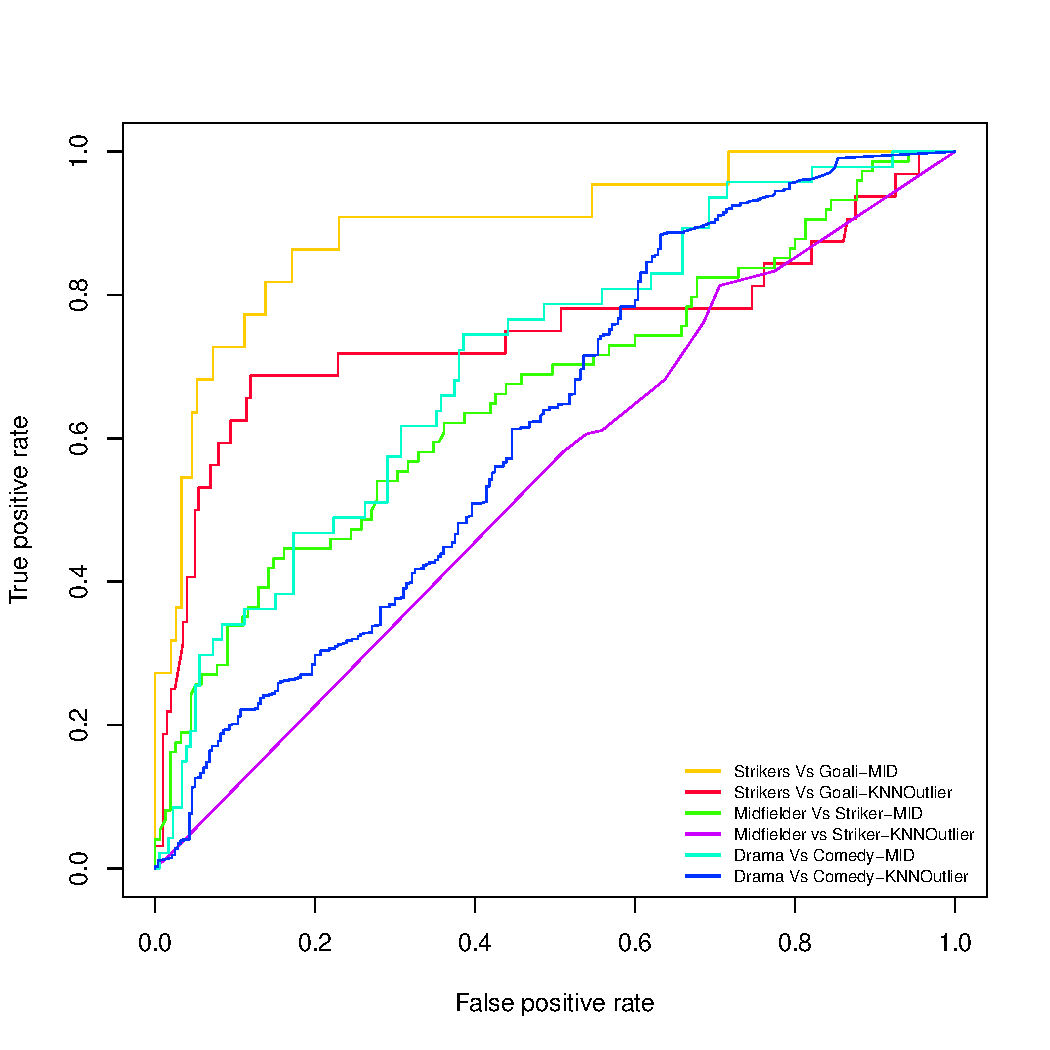
\includegraphics[width=0.5\textwidth] {figures/ROCKNN.pdf}
																		% \caption{Detection Accuracy of $\mid$ vs. $\knn$
																		% \label{fig:ROC}}
																		%\end{figure}
																		%\vspace{-5mm}
																		\paragraph{Strikers vs. Goalies} 
																		$\mid$ separates goalies from Strikers better compared to the other methods.  
																		%
																		In real-world data, a rare object may be a {\em within-class outlier}, i.e., highly anomalous even within its class. In an unsupervised setting without class labels, we do not expect an outlier score to distinguish such an in-class outlier from outliers outside the class. 
																		%								This is the reason why in real-world data, we do not expect an outlier detection score to distinguish the normal class objects perfectly from objects outside the class. 
																		An example is the striker Edin Dzeko. He is a highly anomalous striker who obtains 
																		the top $\mid$ divergence score among both strikers and goalies. His $\mid$ score is highest for the Dribble Efficiency feature. The highest $\mid$ score for that feature occurs when Dribble Efficiency is low, and its parents have the following values: Shot Efficiency high, Tackle Efficiency medium. Looking at the single feature divergence, 
																		%Decomposing this $\mid$ score into feature divergence and joint information divergence, 
																		we see that Edin Dzeko is indeed an outlier in the Dribble Efficiency subspace: His dribble efficiency is low in 16\% of his matches, whereas a randomly selected striker has low dribble efficiency in 50\% of his matches. Thus, Edin Dzeko is an unusually good dribbler. Looking at the mutual information component of $\mid$, i.e., the parent-child correlations, for Edin Dzeko the confidence of the rule 
																		$$\it{ShotEff} = \it{high}, \it{TackleEff} = \it{medium}\rightarrow \it{DribbleEff} = \it{low}$$ is 50\%, whereas in the general striker class it is $38\%$.
																		The $\mid$ divergence also ranks Edin Dzeko as unusual. But because it allows feature and joint information divergence to cancel, his rank is somewhat lower. The likelihood metric does not recognize him as unusual at all. 
																		
																										The next two outliers according to $\mid$ are goalies Paul Robinson and Michel Vorm. Their rank is based only on feature divergence, with zero mutual information distinction. The maximum feature divergence is obtained by the $\it{SavesMade}$ feature. This makes intuitive sense since strikers basically never make saves. 
																		In other words, feature divergence with respect to $\it{SavesMade}$ is a good way to distinguish goalies from strikers. 
																		
																		The $\mid$ divergence also ranks Paul Robinson and Michel Vorm as clear goalies.  The likelihood metric does not recognize Paul Robinson as unusual at all. 
																		%\vspace{-5mm}
																		\paragraph{Midfielders vs. Strikers} 
																		The  $\mid$ metric separates midfielders from strikers better compared than the other methods.  
																		The single feature divergence does not discriminate these two classes of objects. Intuitively, this is because strikers and midfielders are generally similar with respect to single features.  
																		The distance metrics have a better TOR rate than the averaging metrics. 
																		
																			The decomposition analysis for the top three $\mid$ outliers proceeds as follows. 
																		For the single feature score, Robin van Persie is recognized as a clear striker because of the $\it{ShotsOnTarget}$ feature. It makes sense that strikers shoot on target more often than midfielders. Robin van Persie  achieves a high number of shots on targets in $34\%$ of his matches, compared to $3\%$ for a random midfielder. The mutual information component shows that he also exhibits  unusual correlations. For example, 
																		the confidence of the rule
																		$$\it{ShotEff} = \it{high}, \it{TimePlayed} = \it{high} \rightarrow \it{ShotsOnTarget} = \it{high}$$
																		is 70\% for van Persie, whereas for strikers overall it is 52\%.
																		%Both the $\eld$ metric and the $\lnlikelihood$ metric recognize Van Persie as a striker. 
																		
																										Wayne Rooney is recognized as a striker for similar reasons, but less clearly because he achieves a high number of shots on target less frequently. 
																		The most anomalous midfielder is Scott Sinclair. His most unusual feature is $\it{DribbleEfficiency}$: For feature divergence, he achieves a high dribble efficiency $50\%$ of the time, compared to a random midfielder with $30\%$. 
																		%The $\jid$ divergence shows that he also exhibits unusual correlations for DribbleEfficiency.
																		%The $\eld$ divergence too ranks Scott Sinclair as an unusual midfielder, whereas the likelihood method places him in the middle of his class. 
																		%\vspace{-5mm}
																		\paragraph{Drama vs. Comedy} 
																		As with the other datasets, the  $\mid$ metric separates normal objects  from the contrast class better than the other methods.   
																		The top outlier rank is assigned to the within-class outlier $\it{Brave Heart}$. Its most  unusual feature is  $\it{ActorQuality}$: In a random drama movie,  $42\%$ of actors have the highest quality level 4, whereas for $\it{Brave Heart}$ $93\%$ of actors achieve the highest quality level. 
																		%The $\eld$ divergence also ranks $\it{Brave Heart}$ as an unusual drama, whereas the likelihood method places it in the middle of its class. 
																		
																		%based on user assigned ranking. 
																		The  $\mid$ score identifies the comedies  $\it{Blues Brothers}$ and $\it{Austin Powers}$ as the top out-of-class outliers. 
																		%	The main contributor to these rankings is the $\it{Cast\_Position}$ feature. 
																		In a random drama movie,  $49\%$ of actors have casting position 3, whereas for $\it{Austin Powers}$ $78\%$ of actors have this casting position, and for $\it{Blues Brothers}$ $88\%$ of actors do. 
																		%								These three movies also show unusual correlations for this feature with high divergence in the mutual information component (not shown in Table~\ref{table:CaseStudy}).
																		\begin{sidewaystable}
																			\centering
																			\caption{Case study for the top outliers returned by the log-likelihood distance score \mid
																				\label{table:CaseStudy}}
																			\resizebox{1\textwidth}{!}{
																				\begin{tabular}{|l|l|l|l|l|l|} \hline
																					\multicolumn{6}{|c|}{Strikers (Normal) vs. Goalies (Outlier)}\\
																					\hline
																					PlayerName&Position&$\mid$ Rank&$\mid$ Max Node&$\mid$ Node Score&$\fd$ Max feature Value \\ \hline
																					Edin Dzeko&Striker&1&DribbleEfficiency&83.84&DE=low \\ \hline
																					Paul Robinson&Goalie&2&SavesMade&49.4&SM=Medium4\\ \hline
																					Michel Vorm&Goalie&3&SavesMade&85.9&SM=Medium\\ \hline
																					\multicolumn{6}{|c|}{Midfielders (Normal) vs. Strikers (Outlier)}\\
																					\hline
																					PlayerName&Position&$\mid$ Rank&$\mid$ Max Node&$\mid$ Node Score&$\fd$ Max feature Value \\ \hline
																					Robin Van Persie& Striker&1&ShotsOnTarget&153.18&ST=high \\ \hline
																					Wayne Rooney& Striker&2&ShotsOnTarget&113.14&ST=high\\ \hline
																					Scott Sinclair&Midfielder&6&DribbleEfficiency&71.9&DE=high\\ \hline
																					\multicolumn{6}{|c|}{Drama (Normal) vs. Comedy (Outlier)}\\
																					\hline
																					MovieTitle&Genre&$\mid$ Rank&$\mid$ Max Node&$\mid$ Node Score& $\fd$ Max feature Value \\ \hline
																					Brave Heart&Drama&1&ActorQuality&89995.4&a\_quality=4\\ \hline
																					Austin Powers&Comedy&2&Cast\_Position&61021.28&Cast\_Num=3\\ \hline
																					Blue Brothers&Comedy&3&Cast\_Position&24432.21&Cast\_num=3\\ \hline
																				\end{tabular} 
																			}
																		\end{sidewaystable}
																		
																		
																\section{Conclusion}	
																In this chapter, we presented a new approach for applying Bayes nets to object-relational outlier detection. The key idea is to learn one set of parameter values that represent class-level associations, another set to represent object-level associations, and compare how well each parametrization fits the relational data that characterize the target object. The classic metric for comparing two parametrized models is their log-likelihood ratio; we refined this concept to define  a new relational log-likelihood distance metric via two transformations:  (1) a mutual information decomposition, and (2) replacing log-likelihood differences by log-likelihood distances. This metric combines a single feature component, where features are treated as independent, with a correlation component that measures the deviation in the features' mutual information.
																
																In experiments on three synthetic and three real-world outlier sets, the log-likelihood distance achieved the best detection accuracy except for one dataset. The alternative of converting the structured data to a flat data matrix via Propositionalization had a negative impact. %on outlier detection. 
																Case studies showed that the log-distance score leads to easily interpreted rankings.
																%
																Overall, our new log-likelihood distance metric provides a promising new approach for applying machine learning techniques to outlier detection for object-relational data, a challenging and practically important topic. 
																
																
																There are several avenues for future work.  (i) A limitation of our current approach is that it ranks potential outliers, but does not set a threshold for a binary identification of outlier vs. non-outlier. (ii) Our divergence uses expected L1-distance for interpretability, but other distance scores like L2 could be investigated as well. (iii) Extending the expected L1-distance for continuous features is a useful addition. 
																%, and may facilitate combining our object-oriented approach with dimensional hierarchies in an OLAP data cube.
																%Distribution distances other than KLD could be evaluated for outlier detection (e.g., variation distance). However, the KLD variants have special advantages: their asymetry reflects the asymetry between object and class. Also, in a Bayesian network representation of the joint distributions, they decompose into a node-wise sum for easy computation and interpretation. 
																%A promising project for future work would be to combine the object data model and the multi-dimensional model to combine our object outlier method with OLAP-based methods. For example, one could add numeric measures and aggregate attributes to the object model. Another view: convert the object-oriented data to OLAP data, then use their outlier detection.
																
																
																In sum, outlier metrics based on model likelihoods are a new type of structured outlier score for object-relational data.  Our evaluation indicates that this model-based score provides informative, interpretable, and accurate rankings of objects as potential outliers. 
%%% Copyright 1998 Pepe Kubon
%%
%% `one.tex' --- 1st chapter for thes-full.tex, thes-short-tex from
%%                the `csthesis' bundle
%%
%% You are allowed to distribute this file together with all files
%% mentioned in READ.ME.
%%
%% You are not allowed to modify its contents.
%%

%%%%%%%%%%%%%%%%%%%%%%%%%%%%%%%%%%%%%%%%%%%%%%%%%
%
%       Chapter 5
%
%%%%%%%%%%%%%%%%%%%%%%%%%%%%%%%%%%%%%%%%%%%%%%%%

\chapter[Success and Outlierness]{Success and Outlierness}
\label{chap:six}


In chapter~\ref{chap:five} we introduced the $\mid$ metric that quantifies the extent to which the individual association pattern of a potential outlier deviates from that of the whole population. The aim of this chapter is to compare the $\mid$ metric with other meaningful metrics for comparing individuals. The goal is to use the $\mid$ to estimate the value of the individuals and rank them. 
%This goal is achieved in three steps. 1) Individuals are grouped into categories. Categories can be the position of the players (e.g. defender, goalie, striker or midfielder) or the genre of the movies (action, comedy, etc.). 2) Two Bayesian network structures are learned: one from the data for the entire population, the other from individual data. 3) $\mid$  metric is computed using models learned in previous step and then used to rank the individuals.
An empirical evaluation on soccer and movie data shows a strong correlation between the $\mid$ score and success metrics: individuals that our metric identifies as unusual tend to have unusual success.

\section{Introduction}
%Predicting success especially ranking individuals has been a popular topic for statistics/machine learning research in the recent years. 

The appearance of professional soccer statistics websites has made it possible to extend statistical studies to the sports domain. One of the interesting problems in this domain is predicting success and providing true estimates of players' abilities. 
An intuitive way to estimate the value of the players is to manually aggregate information about features of individuals over time and then rank them based on their performance in those features. For example, we can compare players based on the total number of goals they have scored or the average of their shot efficiency. However, this comparison may be unfair to most players because not all players are in the position to shoot or score a goal (e.g. goalies or defenders). One may argue that defenders (or goalies) have some other characteristics that are a lot stronger in their group compared to other groups. However, detecting important and distinctive features of each group of individuals requires domain knowledge and it is not often an easy task.  \\
Another disadvantage of ranking based on manual aggregation of features is that it causes loss of information.
 
 In chapter~\ref{chap:four} and \ref{chap:five} we showed the advantage of using a generative model is to learn complex, and at the same time, informative features for individuals. 
%For instance, by using a generative model, we can find out which relation are associated and which are normally independent of each other. An advantage that can be achieved by using generative models.\\% ne  using number of matches that a player plays becomes important when the player shows high dribble efficiency and pass efficiency.  \\
In this chapter we propose a method to rank individuals which is based on $\mid$ metric introduced in chapter~\ref{chap:five}. We compare the $\mid$ metric to other metrics of success for a given domain. Our reasoning is that high success is an independent metric that indicates an unusual individual. Therefore, a correlation between log-likelihood distance and success is an independent validation of the log likelihood distance and shows that it points to meaningful and interesting outliers. 
%If the model assigns a low likelihood to generating an individual it  says something about that individual and shows how different that individuals is from normal populations. 
%A generic Bayes net (BN) structure is learned with data
%for the entire population. The nodes in the BN represent features
%for links, of multiple types, and attributes of entities,
%also of multiple types. 
%%A difference between relational and
%nonrelational data is that an individual is characterized not
%only by a list of attributes, but also by its links and by attributes
%of the individuals linked to it.
\paragraph{Approach}
Individuals are grouped into categories. A class-model Bayesian network (BN) structure is learned with data for the entire category of the individuals. An individual-model Bayesian network structured is learned  from the individual data. $\mid$ metric is computed based on the approach introduced in chapter \ref{chap:five} and is used to rank the individuals.
\paragraph{Evaluation}
We analyze two real-world data sets, from the UK Premier League and the Internet Movie Database
(IMDb). 
%The empirical distributions of the ELD metric shows that the likelihood ratios highlight individual deviations more strongly.
 Success metrics, such as the player's salary, provide an independent
score for comparison with the ELD score. The empirical distributions of the ELD metric show a strong correlation with independent success metrics.
 \section{Preliminary Analysis}
 Market value of a player is not solely based on the player's performance and is often influenced by some other factors, such as the player's age and nationality.\\
 In this section we study a few of these factors that are known to affect the market value of soccer players in the literature. We manually collected salary, nationality and age of 120 players of the Premier League in order to investigate the effect of each of these factors on the success of players.  
 \paragraph{Fact \#1: Some teams tend to pay more:} Table~\ref{table:salariofDifferentTeam} shows the average salaries of players of different teams in the Premier League. Some teams have much larger
 budgets and are able to pay higher wages compared to less wealthy teams. A player in Manchester United may not necessarily be performing substantially better than a player in the same position in Tottenham, while there is a substantial difference between the average salary of players in Tottenham and Manchester United. For this reason, we normalize the salaries of the player in order to decrease this effect. %Fortunately, after normalization, the difference between averages of salary paid by most of the teams is minor and we can expect this factor to have little effect on predicting the success.
 
%\begin{figure}
%	\centering     %%% not \center
%	{\label{fig:SalaryTeam}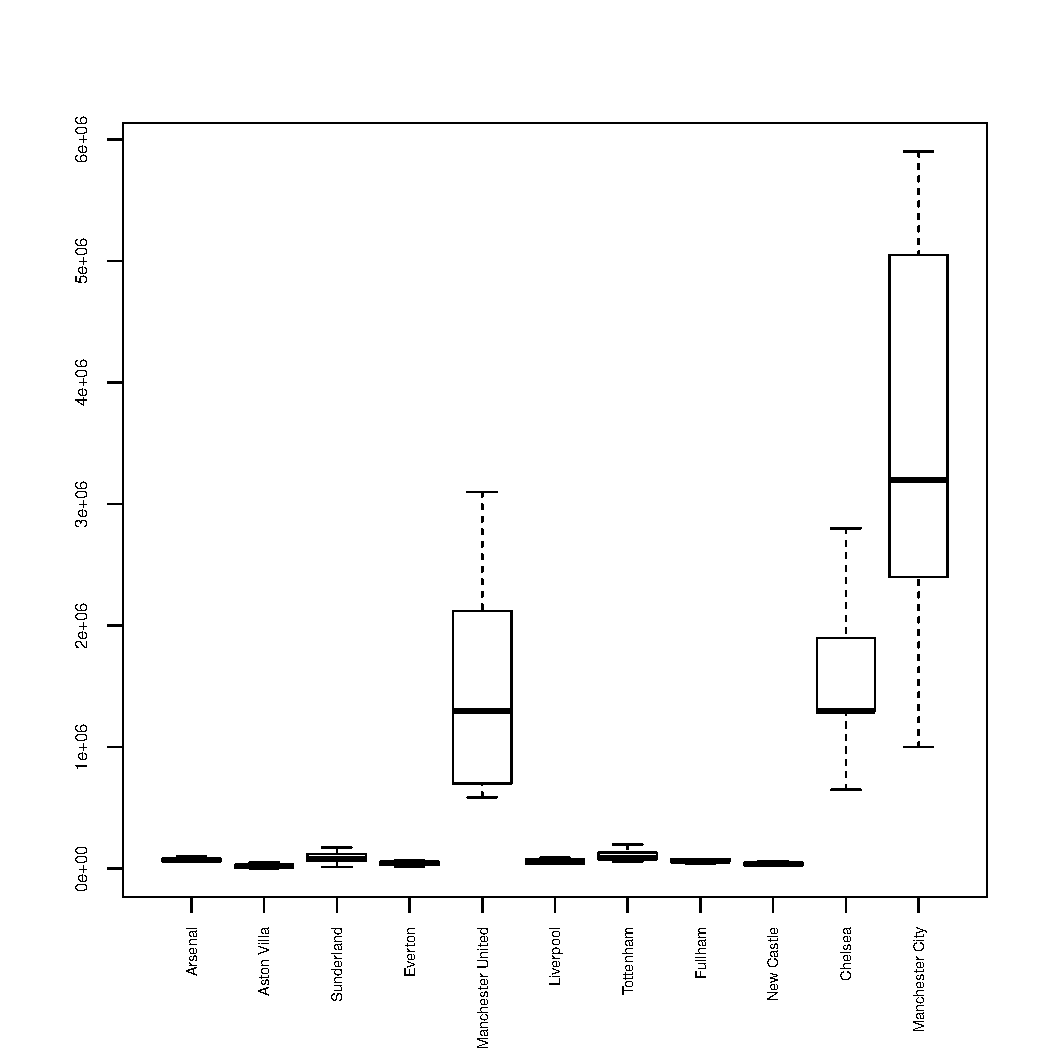
\includegraphics[width=70mm]{figures/TeamSal-2.pdf}}
%%	\subfigure[Wage bill different teams after normalization]{\label{fig:NormalizedSalary}\includegraphics[width=70mm]{figures/TeamNormalSal-2.pdf}}
%	\caption{Salary of the players of different teams}
%\end{figure}



\paragraph{Fact \#2: Player's nationality has little effect on player's salary:} Previous research on soccer shows that the nationality of a player sometimes affects his salary, regardless of his performance~\cite{Wooten2013}. \\
``The phrase `Brazilian soccer player' is like the phrases `French chef' or `Tibetan monk.'  The nationality
expresses an authority, an innate vocation for the job, whatever the natural ability.''~\cite{PAPASTERGIADIS2013}\\
We investigated this phenomenon in our domain and showed that it has very little effect on the player's market value. Figure~\ref{fig:PlayersNormalizedSalary}(a) shows the distribution of salaries of the players across different nationalities.
\begin{table}[htbp]
	
	\centering
	\resizebox{0.6\textwidth}{!}{
		\begin{tabular}{|l|c|}
			\hline
			Team&$\mu$(Salary of the players of PL teams in \euro)\\\hline
			Arsenal&82307.69\\\hline
			Aston Villa&23625.00\\\hline
			Chelsea&88500.00\\\hline
			Everton&44090.91\\\hline
			Fullham&30372.57\\\hline
			Liverpool&66666.67\\\hline
			Manchester City&111076.90\\\hline
			Manchester United&81384.62\\\hline
			New Castle&41000.00\\\hline
			Sunderland&31857.14\\\hline
			Tottenham&65428.57\\\hline
		\end{tabular}}
		%
		\caption{Average salary of players in different teams .\label{table:salariofDifferentTeam}}
	\end{table}

\begin{figure}
	\centering     %%% not \center
	\subfigure[	Salaries of players of different nationalities. ]{\label{fig:SalaryTeam}\includegraphics[width=70mm]{figures/nationalityNormalSal.pdf}}
	\subfigure[	Salaries of players of different age group. ]{\label{fig:b}\includegraphics[width=70mm]{figures/PlayersNormalizedSalary.pdf}}
	\caption{Salary comparison of Premier League Players}\label{fig:PlayersNormalizedSalary}
\end{figure}

%\begin{figure}[t]
%	\centering
%	\includegraphics[width=0.6\textwidth] 
%	{figures/nationalityNormalSal.pdf}
%	\caption{
%		Salaries of players across different nationalities. 
%		\label{fig:nationalitySalary}
%	}
%\end{figure}

\paragraph{Fact \#3: Player's salary increases as age increases:}
Older players, from ages 30 to 33, tend to earn higher wages compared to other age groups because it takes time to accumulate fame and experience. A famous older player and a young player may play equally well, but the famous player may have a higher salary due to his reputation. \\
For each player salary distribution has a different peak, but it is between 30-33 for most players~\cite{schwartz}. Figure~\ref{MetricComputation} shows the salary of the players in different age groups.

Based on the points discussed above, we know that a method that is solely based on players' performance will not be 100\% successful in ranking the players. 
% Please note this fact is not in favour of our method too.

%\begin{figure}[t]
%	\centering
%	\includegraphics[width=0.6\textwidth] 
%	{figures/PlayersNormalizedSalary.pdf}
%	\caption{
%		Salaries of players in different age. 
%		\label{fig:nationalitySalary}
%	}
%\end{figure}
%\begin{figure}[t]
%	\centering
%	\includegraphics[width=0.7\textwidth] 
%	{figures/TeamSal.pdf}
%	\caption{
%		%We show only the Markov blanket of the Results node to simplify. 
%		\label{fig:bns}
%	}
%\end{figure}
%\begin{figure}[t]
%	\centering
%	\includegraphics[width=0.7\textwidth] 
%	{figures/TeamSal.pdf}
%	\caption{
%		%We show only the Markov blanket of the Results node to simplify. 
%		\label{fig:bns}
%	}
%\end{figure}

\section{Related Work }
%Performance assessment is an important tool for operational analysts in many areas. For example, performance of traders or engineers is assessed by fund managers\cite{Grinblatt1989,Swamidass1987}.\\
\subsection{Analyzing sports data}
 Analyzing sports data can make a significant difference in scoring players, signing contracts and preventing injuries. Pei{~\em et al.}\cite{Pei2006} propose a reference-based method that uses relative degree of density with respect to a fixed set of reference points to calculate the neighbourhood density of a data point. They aim to find outstanding players based on two test settings: 1) The total number of games played, goals scored and shooting percentages. 2) Points scored, plus/minus statistics and penalty minus. \\
Schwartz~\cite{schwartz} {~\em et al.} focused on the valuation of draft order in the SuperDraft. The valuation of draft order was first introduced in the National Football League and proved very useful to the coach in trading players. They first estimate career trajectories of players and then assess the value of the draft position by introducing some performance measure. They used time played and salary of the player as ground truth in order to validate their method.

 
\subsection{Ranking system in Sports domain}
Ranking individuals is a useful task for many applications in Information Retrieval, Natural Language Processing and Data mining.
 In sports, performance is usually interpreted as a rating system or ranking system. Ranking players is particularly important in this domain because teams with lower budgets are usually looking for ways to detect undervalued players to be able to compete with wealthier teams for lower costs.
Lewis {\em et. al}~\cite{Lewis2003} used a quantitative analysis to evaluate the value of baseball players. \\
In the individual sports (e.g. tennis), ranking is straightforward and can be driven from the results of past tournaments, as it has been done  for years by the Association of Tennis Professionals (ATP). However, this simple framework for ranking has been questioned and claimed to perform poorly in predicting the results of future games~\cite{McHale2011}. Other sports associations, such as soccer and cricket, also have official rankings of teams and players, which is the basis of many important decisions. For example, FIFA's world ranking plays an important part in awarding work permits to players outside the European Union in the Premier League~\cite{McHale2012}.
 The problem of ranking teams and players is not trivial and the need for a better analytical system should not be understated. Although the world ranking performs poorly in predicting match outcomes, it has been used to determine qualifications for tournaments~\cite{McHale2007}.
 
 In team sports, rating individuals is a more complex task due to team structure; players have different positions. Keri {\em et. al} have developed a rating system for each speciality in baseball~\cite{Keri2006}.
 
 The analysis becomes more complicated when the goal is to compare players with different specialities. Goldman {\em et al.} investigates the metrics that attempt such an analysis in baseball and value players regardless of their position~\cite{Goldman2010}.
 % Lewis 2005 has explored methodologies for such rating system for Cricket. 
  McHale{~\em et. al} developed an index to rate players regardless of their playing speciality, based on their contributions to wining performances~\cite{McHale2012}. 
 


%\section{Experiments}
%We show the distribution of the ELD values on the Soccer and the IMDb datasets.
%
%\subsection{Datasets}
%Similar to the other chapters, data tables are prepared from Opta data~\cite{opta-original} and IMDb~\cite{IMDB-original}. Table~\ref{table:Features} lists the populations and features. Table~\ref{table:Stats} shows summary statistics for the datasets. 
%\begin{table}
%	\centering
%	\resizebox{0.7\textwidth}{!}{
%		\begin{tabular}{|l|l|l|l|} \hline
%			\multicolumn{2}{|c|}{Premier League Statistics}& \multicolumn{2}{|c|}{IMDB Statistics}\\
%			\hline
%			Number Teams&20&Number Movies&3060 \\ \hline
%			Number Players&484&Number Directors&220 \\ \hline
%			Number Matches&380&Number Actors&98690  \\ \hline
%			avg player per match&26.01& avg actor per movie&36.42  \\ \hline
%		\end{tabular} 
%	}
%	\caption{Summary Statistics for the IMDB and Soccer data sets}
%	\label{table:Stats}
%\end{table}
%
%
%\begin{table}[htbp]
%	\centering
%	\resizebox{0.6\textwidth}{!}{
%		\begin{tabular}{|c|p{5cm}|}
%			\hline
%			Individuals & Features\\ \hline
%			\begin{tabular}{c}Soccer-Player\\per Match \end{tabular} & $\it{TimePlayed}$,$\it{Goals}$,$\it{SavesMade}$,
%			$\it{ShotEff}$,$\it{PassEff}$,$\it{WinningGoal}$,
%			$\it{FirstGoal}$,$\it{PositionID}$, $\it{TackleEff}$,$\it{DribbleEff}$,
%			$\it{ShotsOnTarget}$ \\ \hline
%			\begin{tabular}{c}Soccer-Team\\per Match \end{tabular} & $\it{Result}$,$\it{TeamFormation}$,
%			$\sum\it{Goals}$,$\mu\it{ShotEff}$,$\mu\it{PassEff}$,
%			$\mu\it{TackleEff}$,$\mu\it{DribbleEff}$. \\ \hline
%			IMDB-Actor & $\it{Quality}$, $\it{Gender}$ \\ \hline
%			IMDB-Director & $\it{Quality}$,$\it{avgRevenue}$\\ \hline
%			IMDB-Movie&$\it{year}$,$\it{isEnglish}$,$\it{Genre}$,$\it{Country}$, $\it{RunningTime}$, $\it{Rating}$ by User\\ \hline
%			IMDB-User& %$\it{Rating}$,
%			$\it{Gender}$, $\it{Occupation}$.\\ \hline
%		\end{tabular}}
%		\caption{Attribute Features.% $\mu$ = average, $\\sum$ = sum. For relationships please see text.
%			\label{table:Features}}
%		
%	\end{table}
\section{Correlation with Success}
\label{sec:success}

%OS: I put previous writing after \end{document}
%\subsection{Experiments}
%\subsubsection{Datasets}

The aim of this section is to compare the $\mid$ metric with other meaningful metrics for comparing individuals. Our reference metrics are success rankings of individuals selected for a specific domain, shown in table~\ref{table:metrics}. We use the same data as in our other experiments, as described in chapter~\ref{chap:three}. 

Success rankings are one of the most interesting features to users. Strong correlations between the $\mid$ metric and meaningful success metrics provide evidence that the $\mid$ metric is also meaningful. We measure correlation strength by the standard correlation coefficient $\rho$. The coefficient ranges from -1 to 1, where 0 means no correlation and 1 or -1 indicates maximum strength~\cite{Fisher1921}.

The observed correlations are remarkable in at least two respects: 1) The strength of the correlation between the $\mid$ metric and the success ranking are high; coefficients range from 0.45 to 0.82. 2) We observe this phenomenon across different domains, different types of individuals and different success metrics.


\begin{table}[htbp]
	
	\centering
	\resizebox{0.8\textwidth}{!}{
		\begin{tabular}{|l|l|l|l|l|l|}
			\hline
			Dataset&Success Metric&Min&Max&Standard Dev.&Mean\\ \hline
			IMDb & Sum of Rating & 1 & 14795 & 1600.22 & 1057.58\\ \hline
			Soccer-Player &TimePlayed& 5.0 & 3420 & 1015.69 & 1484.0\\ \hline
			Soccer-Player&Normalized Salary&0.007&0.28&0.620&0.100\\\hline
			Soccer-Player&Sum of Shot Efficiency&0&82&9.87&6.53\\\hline
			Soccer-Team &Standing& 1.0 & 20 & 5.91 & 10.5\\ \hline
			
		\end{tabular}}
		\caption{Success metrics and their distributions.\label{table:metrics}}	
	\end{table}
	
	
	
	For a population with a diverse set of skills and resources,
	%apart from a serious decline in quality of generalization, 
	being different from the generic class can be interpreted as both exceptionally better or worse than normal population. In the domains we study in this data, we found that higher $\mid$ scores indicate exceptionally good individuals. Our interpretation of this positive correlation between $\mid$ and success is that our domains featured skilled individuals, such that the average is already quite successful. 
	For example, in the Premier League we expect most players to be in the range of good players. Therefore, deviating from the rest of the population is a signal for detecting exceptionally good players. Our $\mid$-success scatterplots below provide empirical evidence for this interpretation; we typically see a large cluster of individuals around the origin, meaning that their success is normal and their $\mid$ score is low.
	
	\subsection{Methodology}
	
	We report the correlations between the $\mid$ metric and metrics of success for a specific domain. We also focus on some unusually successful individuals as case studies. 
	In considering the correlation between $\mid$ and success, it is useful to investigate subgroups of individuals to ensure an apples-to-apples comparison~\cite{Sun2009}. For instance, the attributes that lead to success are different for strikers and goalies.  Accordingly, we report correlations for subgroups as well as entire classes of individuals. 
	
	%	Another point to consider is that, in BN generalization, similar to statistical generalization, population size and the structure of the  individuals is important. For example, in the Premier League, when the goal is to predict the success of  teams, there is no strong correlation between the ELD metric and standing of the teams as we expected it to be similar to the other domain/individuals ($\rho(Standing, ELD)=-0.21$). This could be due to the diverse and yet very small population (20 teams in total). But when we decrease diversity by evaluation only top 10 teams in the Premier League standing, correlation becomes a lot more stronger ($\rho(Standing, ELD)=-0.71$).
	
	
	\subsection{Correlations between the $\mid$ outlier metric and success}
	
	The next three tables summarize the observed correlations between success and $\mid$ metrics: Teams in Table~\ref{table:teamELD}, Players in Table~\ref{table:ELDwithPlayer},  Movies in Table~\ref{table:ELDmovie}.

		
		
		
		%\begin{table}[htbp]
		%	\caption{Correlation between $\mid$ metric and success metric of Goalies . \textbf{make single table. Probably make the rows the metrics, the columns the classes, including the whole population. Or add a row for all players. See our aaa2014.tex paper. } \label{table:players}}
		%	\centering
		%	\resizebox{0.7\textwidth}{!}{
		%		\begin{tabular}{|c|c|c|c|}
		%			\hline
		%			Metric&Sum of SavesMade&TimePlayed&Salary\\\hline
		%			$\mid$&0.71&0.73&0.6\\\hline
		%		\end{tabular}}
		%		\caption{Correlation between $\mid$ metric and success metric of Midfielders. \label{table:Midfielders}}
		%		\resizebox{1\textwidth}{!}{
		%			\begin{tabular}{|c|c|c|c|c|}
		%				\hline
		%		Metric&Sum of Pass Efficiency&Sum of dribble Efficiency&TimePlayed&Salary\\\hline
		%		$\mid$&0.89&0.76&0.80&0.45\\\hline
		%			\end{tabular}
		%			
		%			}
		%				\caption{Correlation between $\mid$ metric and success metric of Strikers .\label{table:strikers}}
		%					\resizebox{0.7\textwidth}{!}{
		%						\begin{tabular}{|c|c|c|c|}
		%							\hline
		%							Metric&Shots On Target&TimePlayed& Salary\\\hline
		%							$\mid$&0.72&0.82&0.79\\\hline
		%						\end{tabular}
		%						
		%					}
		%\caption{Correlation between $\mid$ metric and success metric of Movies .\label{table:movie}}
		%\resizebox{0.8\textwidth}{!}{
		%	\begin{tabular}{|c|c|c|c|}
		%		\hline
		%	Genre&Sum of Rating&Average of Rating&Number of Rating\\\hline
		%	Action&0.68&0.30&0.72\\\hline
		%	Drama&0.78&0.29&0.81\\\hline
		%	Comedy&0.85&0.41&0.84\\\hline
		%	All Movies&0.56&0.17&0.60\\\hline
		%		\end{tabular}
		%}
		%		\end{table}
		%		
		%
		
		\begin{table}
			\caption{Correlation between $\mid$ metric and success metric of Movies.\label{table:ELDmovie}}
			\centering
			\resizebox{0.8\textwidth}{!}{
				\begin{tabular}{|c|c|c|c|}
					\hline
					Genre&Sum of Rating&Average of Rating&Number of Rating\\\hline
					Action&0.68&0.30&0.72\\\hline
					Drama&0.76&0.32&0.77\\\hline
					Comedy&0.85&0.41&0.84\\\hline
					All Movies&0.56&0.17&0.60\\\hline
				\end{tabular}
			}
		\end{table}
		
		
			
			\begin{table}
				\caption{Correlation between $\mid$ metric and standing of Teams. The best standing is place 1. \label{table:teamELD}}
				\centering
				\resizebox{0.4\textwidth}{!}{
					\begin{tabular}{|c|c|}
						\hline
						Team&Standing\\\hline
						Top Teams&-0.71\\\hline
						Bottom Team&-0.33\\\hline
						All Team&-0.20\\\hline
					\end{tabular}
				}
			\end{table}
			
			
			\begin{table}
				\caption{Correlation between $\mid$ metric and success metrics of Players.}
				\label{table:ELDwithPlayer}
				\centering
				\resizebox{1\textwidth}{!}{
					\begin{tabular}{|c|c|c|c|c|c|}
						\hline
						Class&TimePlayed&Salary&SavesMade&ShotsOntarget&Passeff\\\hline
						Strikers&0.76&0.79&NA&0.72&NA\\\hline
						Midfielders&0.73&0.45&NA&NA&0.89\\\hline
						Goalies&0.69&NA&0.71&NA&NA\\\hline
						All players&0.81&0.56&NA&NA&NA\\\hline
						%Synthetic&40&280\\ \hline
					\end{tabular}}
					
				\end{table}
		
		
		\subsubsection{Teams} 
		\paragraph{Team Standing}
		The most successful team has Standing=1 and the least successful team has Standing=20 in the 2011-2012 Season. For the top teams, a very strong negative correlation emerges between $\mid$ and standing: teams with higher $\mid$ achieve a better (lower) standing. 
		
		Figure~\ref{fig:TeamStandingELD} shows the correlation of $\mid$ with team success metrics in a scatter plot. The top two teams, Manchester City and Manchester United, stand out strongly in terms of the $\mid$ metric (bottom right corner).
		
		\begin{figure}[t]
			\centering
			\includegraphics[width=0.5\textwidth]{NewPlotsJan2016/topTeamStats-Sep.pdf}
			
			\caption{Teams: Team Standing vs. $\mid$ for the top teams in the Premier League. 
				\label{fig:TeamStandingELD}}
		\end{figure}
		
		\subsubsection{Players}
		
		\paragraph{Players Time Played} is the total time that a player played over all matches in the season. This metric was shown to correlate strongly with other success metrics, such as salary, on MLS soccer data~\cite{schwartz}. 
		%	Tables ~\ref{table:goalie} and \ref{table:players} 
		%	
		%	and Figures \ref{fig:GoalieTime} and \ref{fig:StrikerTime} 
		%	
		%	show the correlation between the ELD metric and time played. 
		For each subgroup there is a strong positive correlation with $\mid$, meaning that atypical players with higher $\mid$ tend to play more minutes.
		
		%The results are mixed; they show that pay cannot be adequately explained by past performance
		%	alone, nor are pay levels justified by future performance. The bids for players in the initial
		%	auction appear to have been based on intangibles that are hard to quantify%
		\paragraph{Salary} is probably the most obvious, and at the same time often the most misleading way to measure success of the players. Previous studies suggest that salary of the players does not  always follow their performance in many sports, such as baseball and soccer~\cite{Hall2002,Barrio2004}. They show that pay cannot be explained only by past performance and there are other factors that are hard to quantify and have a great effect on the salaries. 
		
		We manually collected the salaries of 120 players that we could find on-line. Table \ref{table:ELDwithPlayer}  and Figures~\ref{fig:strikersELD} and \ref{fig:goaliesELD} show the correlation between $\mid$ and this success metric. The correlation is high, especially for Strikers. We discuss the relatively weaker salary correlation for midfielders in more detail below.
		
		\paragraph{Shots on Target} applies to strikers only. This is defined as any shot attempt that would, or does, enter the goal if left unblocked. We record the total number of these shots over all matches of the strikers only. This metric was shown to correlate strongly with $\mid$ (see Table \ref{table:ELDwithPlayer}, Figure~\ref{fig:StrikerShot}).
		
		Figure~\ref{fig:strikersELD} plots $\mid$ against striker success metrics. We observe a large cluster around the origin, which points to a large base of normal strikers with both salaries and low $\mid$ scores. %The striker with the greatest $\mid$ score is Robin van Persie; he stands out in terms of Shots on Target, Time Played, and Salary. 
		
		%should probably label the points with individual names
		
		
		\begin{figure}
			\centering     %%% not \center
			\subfigure[Strikers: Salary vs $\mid$. ]{\label{fig:StrikerSalary}\includegraphics[width=0.48\textwidth]{NewPlotsJan2016/1d-sumStrikerSalary.pdf}}
			\subfigure[Strikers: Shots On Target vs $\mid$]{\label{fig:StrikerShot}\includegraphics[width=0.5\textwidth]{NewPlotsJan2016/1d-ShotsonTarget-sumStrikerStatistics.pdf}}
			\subfigure[Strikers: Time played vs $\mid$.]{\label{fig:StrikerTime}\includegraphics[width=0.5\textwidth]{NewPlotsJan2016/1d-sumStrikerStatistics.pdf}}
			\caption{Correlations in the strikers population\label{fig:strikersELD}}
		\end{figure}
		
		
		
		\paragraph{Saves Made} applies to goalies only; it is defined as the total number of saves that goalies made over all the matches. This metric shows a strong correlation with $\mid$ as well (see Table~\ref{table:ELDwithPlayer}, Figure~\ref{fig:GoalieSaves}).  
		
		Figure~\ref{fig:goaliesELD} shows the correlation of $\mid$ with goalie success metrics in a scatter plot. Goalies do not vary much in terms of the time they play. Wayne Hennessey has the highest number of Saves Made and also an unusually high $\mid$ score, although not the highest. 
		
		
		
		\begin{figure}
			\centering     %%% not \center
			\subfigure[Goalies: sum of time played vs $\mid$. ]{\label{fig:GoalieTime}\includegraphics[width=0.48\textwidth]{NewPlotsJan2016/sumGoalieStatistics.pdf}}
			\subfigure[Goalies: sum of saves made vs $\mid$]{\label{fig:GoalieSaves}\includegraphics[width=0.5\textwidth]{NewPlotsJan2016/sumGoalieStatisticsSavesMade.pdf}}
			%	\subfigure[Teams: Team Standing vs. $\mid$ for the top teams in Premier League. \textbf{separate figure please}]{\label{fig:TeamStanding}\includegraphics[width=0.5\textwidth]{NewPlotsJan2016/topTeamStats.pdf}}
			\caption{Correlations in the goalies population\label{fig:goaliesELD}}
		\end{figure}
		
		
		\paragraph{Midfielder Salary} 
		
		We omit a scatterplot for midfielder salary vs. $\mid$ because it is less informative due to the weaker  correlation (0.45).
		%
		%While there is a strong correlation between salary of the Strikers and ELD score (0.79), this correlation becomes weaker in the Goalie population and even less apparent in Midfielder group. 
		To investigate the reason for the weaker correlation, we chose two midfielders: 1) Stephane Sessegnon  who has been ranked second in the $\mid$ ranking but does not draw a large salary and 2) Steven Gerrard is a very well known player and ranked second in the Salary ranking, but according to the $\mid$ score, he has been ranked 21. Based on domain knowledge, we chose some of the features from the raw data that are relevant to midfield performance and compared the feature statistics for these two players. Table~\ref{table:MidfielderComparison} shows the details of their appearances in different matches. Sessegnon scored higher than Gerrard in three out of the four categories (Passes and Time Played). However, his salary was much lower than Gerrard's. This is an example of how weak the correlation is between salary and the observed box scores, which is the basis for the $\mid$ metric. 
		%to show how unfair and unreliable the salary is in this domain.
		%	 Unsuccessful Passes&Successful Long Passes
		\begin{table}[htbp]
			
			\centering
			\resizebox{1\textwidth}{!}{
				\begin{tabular}{|l|l|c|c|c|c|c|c|c|}
					\hline
					Name&Team&age&\begin{tabular}{c}Salary\\Ranking \end{tabular}&\begin{tabular}{c}$\mid$\\Ranking \end{tabular}&\begin{tabular}{c}Time\\Played \end{tabular}&\begin{tabular}{c}Unsuccessful\\Passes \end{tabular}&\begin{tabular}{c}Successful\\Long Passes \end{tabular}&\begin{tabular}{c}Successful\\corners \end{tabular}\\\hline
					Steven Gerrard	&Liverpool&31&2&21&1212 min&244&52&25\\\hline
					Stephane Sessegnon&Sunderland&26&22&2&3133 min&231&82&15\\\hline
					
					%	$\mid$&0.71&0.73&0.6\\\hline
				\end{tabular}}
				%
				\caption{Comparison of two midfielders.\label{table:MidfielderComparison}}
			\end{table}
			
			
			\subsubsection{Movies} 
			
			\paragraph{Movie Sum of Ratings} is the number of user ratings of a movie. Table~\ref{table:ELDmovie} shows a high correlation with the $\mid$ metric. The highest correlation obtained is for the Comedy genre (0.85). 
			%See Figure~\ref{fig:ActionRate},Figure~\ref{fig:ComedyRate}, Figure~\ref{fig:DramaRate}). 
			The correlation between a movie and the sum of its ratings is equally strong, but the correlation with its average rating is much weaker. Thus, the $\mid$ score is mainly related to how many users have rated the movie rather than with how they have rated it. The number of ratings is a meaningful success metric as it indicates the number of people who have gone to see a movie.  
			
			
			Figure~\ref{fig:Movies} shows the correlation of $\mid$ with movie success metrics in a scatter plot. We again observe a large cluster of movies around the origin. For drama and comedy movies, the top rated movies are (``American Beauty'' resp. ``Being John Malkovich''); these also stand out in the $\mid$ metric. 
			
			
			\begin{figure}
				\centering     %%% not \center
				\subfigure[Action movies: sum of ratings by users vs $\mid$. ]{\label{fig:ActionRate}\includegraphics[width=0.48\textwidth]{NewPlotsJan2016/Action-Correlation.pdf}}
				\subfigure[Comedy movies: sum of ratings by users vs $\mid$]{\label{fig:ComedyRate}\includegraphics[width=0.5\textwidth]{NewPlotsJan2016/Comedy-Correlation.pdf}}
				\subfigure[Drama movies: sum of ratings by users vs $\mid$.]{\label{fig:DramaRate}\includegraphics[width=0.5\textwidth]{NewPlotsJan2016/Drama-Correlation.pdf}}
				\caption{Correlation in the movies population\label{fig:Movies}}
			\end{figure}
			
			
\section{Conclusion}
In this chapter we used the $\mid$ metric, that was introduced in chapter~\ref{chap:five}, to rank the individuals. We compared the $\mid$ metric to other metrics of success for a given domain.
In our experimental results we showed that the $\mid$ metric correlates with success metrics, to a surprising degree, across different domains and classes of individuals. Since high success is an independent metric that indicates an unusual individuals, this correlation shows that $\mid$ marks meaningful and interesting outliers.

We investigated some independent factors that affect the success of individuals in the Premier League. We showed that there are factors other than the performance of players that affect their ranking and for this reason the methods that are solely based on evaluation of the performance of players can never achieve 100$\%$ accuracy in predicting the ranking. 


%\paragraph{Soccer Data} 
%The Opta data were released by Manchester City. 
%It lists all the ball actions within each game by each player, for the 2011-2012 season. 
%%The data consists of information about the actions of a single player in a given match 
%%from 2011 to 2012. 
%%Number of goals, passes, fouls, tackles, saves and blocks and also position 
%%assigned to a player in a match are examples of the information associated with each player. [list]
%%Information about the teams in a season, such as number of home wins, draws or away wins can be extracted by massaging the data. 
%%[The information can be visualized as a heterogeneous network that links players to teams, and teams to matches. ]
%For each player in a match, our data set contains eleven player features.
%% like $\it{TimePlayed}(\P,\M)$.
%For each team in a match, there are five features computed as player feature aggregates, as well as the team formation and the result (win, tie, loss). 
%There are two relationship terms, $\it{Appears\_Player}(\P,\M)$, $\it{Appears\_Team}(\T,\M)$. We store the data in a relational database, with a table for each base population and a table for each relationship.

%Six team f aggregates of player features. 
% like $\it{shoteff}(\team,\match)$. 
%The 11 player features are \\ 
%
%$\it{TimePlayed}$, $\it{SavesMade}$, $\it{ShotEff}$,
% $\it{FirstGoal}$, $\it{WinningGoal}$, $\it{Goals}$,$\it{PositionID}$, $\it{PassEff}$, $\it{TackleEff}$,$\it{DribbleEff}$,
% $\it{ShotsOnTarget}$\\
%
%\paragraph{IMDB Data} 
%
%The Internet Movie Database (IMDB) is an online database of information related to films, television programs, and video games.
%The IMDB website offers a dataset containing a information on cast, crew, titles, technical details and biographies into a set of compressed text files. 
%We preprocessed the data \cite{Peralta2007} to obtain a database with seven tables: one for each population and one for the three relationships $\it{Rated}(\user,\movie)$, $\it{Directs}(\director,\movie)$, and $\it{ActsIn}(\actor,\movie)$.

	
%\section{Likelihood Ratio and Success Metrics}
%The aim of this section is to compare the ELD metric with other meaningful success metrics for comparing individuals. Our reference metrics are success rankings of individuals, shown in table~\ref{table:successmetrics}. Strong correlations between the ELD metric and meaningful success metrics provide evidence that the ELD metric is meaningful as well. We measure correlation strength by the standard correlation coefficient $\rho$. The coefficient ranges from -1 to 1, where 0 means no correlation and 1 or -1 indicates maximum strength~\cite{Fisher1921}.\\
%
%Correlations are remarkable in at least two respects. 1) the strength of the correlation between the ELD metric and the success ranking are high: coefficients range from 0.3 to 0.82. (Oliver: correlation between ELD and movie rank is not as high as sum of ratings, should we just drop that or keep it? see table~\ref{table:movie}). 2) The trend holds across two different domains, different types of individuals and different success metrics. 
%\begin{table}[htbp]
%	
%	\centering
%	\resizebox{0.8\textwidth}{!}{
%		\begin{tabular}{|l|l|l|l|l|l|}
%			\hline
%			Dataset&Success Metric&Min&Max&Standard Dev.&Mean\\ \hline
%			IMDb & Sum of Rating & 1.8 & 9 & 1.14 & 6.3\\ \hline
%			Soccer-Player &TimePlayed& 5.0 & 3420 & 1015.69 & 1484.0\\ \hline
%			Soccer-Player&Normalized Salary&s&s&s&s\\\hline
%			Soccer-Player&Sum of Shot Efficiency&s&s&s&s\\\hline
%			Soccer-Team &Sum of Score& 1.0 & 20 & 5.91 & 10.5\\ \hline
%			
%		\end{tabular}}
%		\caption{Success metrics. \label{table:metrics}}
%		
%	\end{table}
%
%The quality of generalization of population is the key to the performance of ELD metric in ranking individuals. For example, in Premier League we expect most players to be in the range of good players. So the more different a player is from the population we can interpret it as a sign of detecting exceptionally good players. If we have a more diverse population in terms of performance, apart from a serious decline in quality of generation, being different from generic model can be interpreted as both exceptionally better or worst than normal population.\\
%Another point to consider is that, in BN generalization, similar to statistical generalization, population size and the structure of the  individuals is important. For example, in the Premier League, when the goal is to predict the success of  teams, there is no strong correlation between the ELD metric and standing of the teams as we expected it to be similar to the other domain/individuals ($\rho(Standing, ELD)=-0.21$). This could be due to the diverse and yet very small population (20 teams in total). But when we decrease diversity by considering only top 10 teams in our evaluation, correlation becomes a lot more stronger ($\rho(Standing, ELD)=-0.71$).
%\paragraph{Team Standing}
%The most successful team has Standing=1 and the least successful team has Standing=20. If we distinguish top teams in the standing, a strong negative correlation emerges between ELD and standing: teams with higher ELD achieve a better(lower) standing. Figure~\ref{fig:teamStanding} shows the scatter plot of this correlation and its best fit regression line.
%\paragraph{Players Time Played} is the total time that a player played over all matches in the season. This metric was shown to correlate strongly with other success metrics, such as salary, on MLS soccer data~\cite{schwartz}. Tables ~\ref{table:goalie} and \ref{table:strikers} and Figures \ref{fig:GoalieTime} and \ref{fig:StrikerTime} show the correlation between the ELD metric and time played. For the the entire population there is a strong positive correlation meaning that atypical players with higher ELD tend to play more minutes.
%\paragraph{Salary} is probably the most obvious way of comparing players. We manually collected salary of some Strikers that we could find on-line. Table \ref{table:strikers}  and Figures~\ref{fig:NormalizedSalary} show the correlation between ELD and this success metric.
%\paragraph{Shots on Target} is any shot attempt that would or does enter the goal if left unblocked. We record total number these shots over all matches of the players. This metric was shown to correlate strongly with ELD (see Table \ref{table:strikers}, Figure~\ref{fig:StrikerShot}).
%\paragraph{Saves Made} is total number of saves that goalies had made over all the matches. This metric has been used as another success metric for Goalies' population and shows a strong correlation as well(see Table ~\ref{table:goalie}, Figure\ref{fig:GoalieSaves}).  
%\paragraph{Movie Rating} is the sum of user rating of the movies. For the movies in different Genre this metric shows a high correlation with the ELD metric (see Table~\ref{table:movie}, Figure~\ref{fig:ActionRate},Figure~\ref{fig:ComedyRate}, Figure~\ref{fig:DramaRate}).
%\begin{table}[htbp]
%	
%	\centering
%	\resizebox{0.7\textwidth}{!}{
%		\begin{tabular}{|c|c|c|}
%			\hline
%		Metric&Sum of SavesMade&TimePlayed\\\hline
%		ELD&0.71&0.73\\\hline
%		\end{tabular}}
%		%
%		\caption{Correlation between ELD metric and success metric of Goalies .\label{table:goalie}}
%	\end{table}
%	
%	\begin{table}[htbp]
%		
%		\centering
%		\resizebox{0.7\textwidth}{!}{
%			\begin{tabular}{|c|c|c|c|}
%				\hline
%				Metric&Shots On Target&TimePlayed& Salary\\\hline
%				ELD&0.72&0.82&0.79\\\hline
%			\end{tabular}}
%			%
%			\caption{Correlation between ELD metric and success metric of Strikers .\label{table:strikers}}
%		\end{table}
%		
%			
%			\begin{table}[htbp]
%				
%				\centering
%				\resizebox{0.5\textwidth}{!}{
%					\begin{tabular}{|c|c|c|}
%						\hline
%						Genre&Sum of Rating&Movie Rank\\\hline
%						Action&0.68&0.30\\\hline
%						Drama&0.78&0.31\\\hline
%						Comedy&0.85&0.42\\\hline
%				\end{tabular}}
%					%
%					\caption{Correlation between ELD metric and success metric of Movies .\label{table:movie}}
%				\end{table}
%				
%%	\begin{figure}[t]
%%		\centering
%%		\includegraphics[width=0.8\textwidth] 
%%		{correlations/Drama-Correlation.pdf}
%%		\caption{
%%			Salaries of players across different nationalities. 
%%			\label{fig:nationalitySalary}
%%		}
%%	\end{figure}			
%%\begin{figure}
%\begin{figure}
%	\centering
%	\begin{minipage}{0.45\linewidth}
%		\centering
%		\includegraphics[width=3.0in]{Correlation-SimplePlots/1d-sumStrikerSalary.pdf}
%		\caption{Strikers: Salary vs ELD}
%		\label{fig:StrikerSalary}
%	\end{minipage}
%	\hspace{0.05\linewidth}
%		\begin{minipage}{0.45\linewidth}
%			\centering
%			\includegraphics[width=3.0in]{Correlation-SimplePlots/1d-ShotsonTarget-sumStrikerStatistics.pdf}
%			\caption{Strikers: Shots On Target vs ELD}
%			\label{fig:StrikerShot}
%		\end{minipage}
%			\hspace{0.05\linewidth}
%			\begin{minipage}{0.45\linewidth}
%				\centering
%				\includegraphics[width=3.0in]{Correlation-SimplePlots/1d-sumStrikerStatistics.pdf}
%				\caption{Strikers: Time played vs ELD}
%				\label{fig:StrikerTime}
%			\end{minipage}
%\end{figure}
%
%\begin{figure}
%	\centering
%	\begin{minipage}{0.45\linewidth}
%		\centering
%		\includegraphics[width=3.0in]{Correlation-SimplePlots/Action-Correlation.pdf}
%		\caption{Action movies: sum of ratings by users vs ELD}
%		\label{fig:ActionRate}
%	\end{minipage}
%	\hspace{0.05\linewidth}
%	\begin{minipage}{0.45\linewidth}
%		\centering
%		\includegraphics[width=3.0in]{Correlation-SimplePlots/Comedy-Correlation.pdf}
%		\caption{Comedy movies: sum of ratings by users vs ELD}
%		\label{fig:ComedyRate}
%	\end{minipage}
%	\hspace{0.05\linewidth}
%	\begin{minipage}{0.45\linewidth}
%		\centering
%		\includegraphics[width=3.0in]{Correlation-SimplePlots/Drama-Correlation.pdf}
%		\caption{Drama movies: sum of ratings by users vs ELD}
%		\label{fig:DramaRate}
%	\end{minipage}
%\end{figure}
%
%				
%				
%				
%				\begin{figure}
%					\centering
%					\begin{minipage}{0.45\linewidth}
%						\centering
%						\includegraphics[width=3.0in]{Correlation-SimplePlots/TeamStanding.pdf}
%						\caption{Teams: Correlation between team's Standing and ELD for the top teams in Premier League standing}
%						\label{fig:teamStanding}
%					\end{minipage}
%					\hspace{0.05\linewidth}
%					\begin{minipage}{0.45\linewidth}
%						\centering
%						\includegraphics[width=3.0in]{Correlation-SimplePlots/sumGoalieStatistics.pdf}
%						\caption{Goalies: sum of time played vs ELD}
%						\label{fig:GoalieTime}
%					\end{minipage}
%					\hspace{0.05\linewidth}
%					\begin{minipage}{0.45\linewidth}
%						\centering
%						\includegraphics[width=3.0in]{Correlation-SimplePlots/sumGoalieStatisticsSavesMade.pdf}
%						\caption{Goalies: sum of saves made by users vs ELD}
%						\label{fig:GoalieSaves}
%					\end{minipage}
%				\end{figure}
%				
				
				
%					\begin{figure}[t]
%						\centering
%						\includegraphics[width=0.45\textwidth] 
%						{Correlation-SimplePlots/topTeamStats.pdf}
%						\caption{
%							Teams: Correlation between team's performance and ELD. 
%							\label{fig:nationalitySalary}
%						}
%					\end{figure}

%	\centering     %%% not \center
%	\subfigure[Figure A]{\label{fig:a}\includegraphics[width=60mm]{figures/SeasonGraph.pdf}}
%	\subfigure[Figure B]{\label{fig:b}\includegraphics[width=60mm]{figures/SeasonGraph.pdf}}
%	\caption{my caption}
%\end{figure}

%% Copyright 1998 Pepe Kubon
%%
%% `one.tex' --- 1st chapter for thes-full.tex, thes-short-tex from
%%                the `csthesis' bundle
%%
%% You are allowed to distribute this file together with all files
%% mentioned in READ.ME.
%%
%% You are not allowed to modify its contents.
%%

%%%%%%%%%%%%%%%%%%%%%%%%%%%%%%%%%%%%%%%%%%%%%%%%%
%
%       Chapter 5
%
%%%%%%%%%%%%%%%%%%%%%%%%%%%%%%%%%%%%%%%%%%%%%%%%

\chapter[Success and Outlierness]{Success and Outlierness}
\label{chap:six}


In chapter~\ref{chap:five} we introduced the $\mid$ metric that quantifies the extent to which the individual association pattern of a potential outlier deviates from that of the whole population. The aim of this chapter is to compare the $\mid$ metric with other meaningful metrics for comparing individuals. The goal is to use the $\mid$ to estimate the value of the individuals and rank them. 
%This goal is achieved in three steps. 1) Individuals are grouped into categories. Categories can be the position of the players (e.g. defender, goalie, striker or midfielder) or the genre of the movies (action, comedy, etc.). 2) Two Bayesian network structures are learned: one from the data for the entire population, the other from individual data. 3) $\mid$  metric is computed using models learned in previous step and then used to rank the individuals.
An empirical evaluation on soccer and movie data shows a strong correlation between the $\mid$ score and success metrics: individuals that our metric identifies as unusual tend to have unusual success.

\section{Introduction}
%Predicting success especially ranking individuals has been a popular topic for statistics/machine learning research in the recent years. 

The appearance of professional soccer statistics websites has made it possible to extend statistical studies to the sports domain. One of the interesting problems in this domain is predicting success and providing true estimates of players' abilities. 
An intuitive way to estimate the value of the players is to manually aggregate information about features of individuals over time and then rank them based on their performance in those features. For example, we can compare players based on the total number of goals they have scored or the average of their shot efficiency. However, this comparison may be unfair to most players because not all players are in the position to shoot or score a goal (e.g. goalies or defenders). One may argue that defenders (or goalies) have some other characteristics that are a lot stronger in their group compared to other groups. However, detecting important and distinctive features of each group of individuals requires domain knowledge and it is not often an easy task.  \\
Another disadvantage of ranking based on manual aggregation of features is that it causes loss of information.
 
 In chapter~\ref{chap:four} and \ref{chap:five} we showed the advantage of using a generative model is to learn complex, and at the same time, informative features for individuals. 
%For instance, by using a generative model, we can find out which relation are associated and which are normally independent of each other. An advantage that can be achieved by using generative models.\\% ne  using number of matches that a player plays becomes important when the player shows high dribble efficiency and pass efficiency.  \\
In this chapter we propose a method to rank individuals which is based on $\mid$ metric introduced in chapter~\ref{chap:five}. We compare the $\mid$ metric to other metrics of success for a given domain. Our reasoning is that high success is an independent metric that indicates an unusual individual. Therefore, a correlation between log-likelihood distance and success is an independent validation of the log likelihood distance and shows that it points to meaningful and interesting outliers. 
%If the model assigns a low likelihood to generating an individual it  says something about that individual and shows how different that individuals is from normal populations. 
%A generic Bayes net (BN) structure is learned with data
%for the entire population. The nodes in the BN represent features
%for links, of multiple types, and attributes of entities,
%also of multiple types. 
%%A difference between relational and
%nonrelational data is that an individual is characterized not
%only by a list of attributes, but also by its links and by attributes
%of the individuals linked to it.
\paragraph{Approach}
Individuals are grouped into categories. A class-model Bayesian network (BN) structure is learned with data for the entire category of the individuals. An individual-model Bayesian network structured is learned  from the individual data. $\mid$ metric is computed based on the approach introduced in chapter \ref{chap:five} and is used to rank the individuals.
\paragraph{Evaluation}
We analyze two real-world data sets, from the UK Premier League and the Internet Movie Database
(IMDb). 
%The empirical distributions of the ELD metric shows that the likelihood ratios highlight individual deviations more strongly.
 Success metrics, such as the player's salary, provide an independent
score for comparison with the ELD score. The empirical distributions of the ELD metric show a strong correlation with independent success metrics.
 \section{Preliminary Analysis}
 Market value of a player is not solely based on the player's performance and is often influenced by some other factors, such as the player's age and nationality.\\
 In this section we study a few of these factors that are known to affect the market value of soccer players in the literature. We manually collected salary, nationality and age of 120 players of the Premier League in order to investigate the effect of each of these factors on the success of players.  
 \paragraph{Fact \#1: Some teams tend to pay more:} Table~\ref{table:salariofDifferentTeam} shows the average salaries of players of different teams in the Premier League. Some teams have much larger
 budgets and are able to pay higher wages compared to less wealthy teams. A player in Manchester United may not necessarily be performing substantially better than a player in the same position in Tottenham, while there is a substantial difference between the average salary of players in Tottenham and Manchester United. For this reason, we normalize the salaries of the player in order to decrease this effect. %Fortunately, after normalization, the difference between averages of salary paid by most of the teams is minor and we can expect this factor to have little effect on predicting the success.
 
%\begin{figure}
%	\centering     %%% not \center
%	{\label{fig:SalaryTeam}\includegraphics[width=70mm]{figures/TeamSal-2.pdf}}
%%	\subfigure[Wage bill different teams after normalization]{\label{fig:NormalizedSalary}\includegraphics[width=70mm]{figures/TeamNormalSal-2.pdf}}
%	\caption{Salary of the players of different teams}
%\end{figure}



\paragraph{Fact \#2: Player's nationality has little effect on player's salary:} Previous research on soccer shows that the nationality of a player sometimes affects his salary, regardless of his performance~\cite{Wooten2013}. \\
``The phrase `Brazilian soccer player' is like the phrases `French chef' or `Tibetan monk.'  The nationality
expresses an authority, an innate vocation for the job, whatever the natural ability.''~\cite{PAPASTERGIADIS2013}\\
We investigated this phenomenon in our domain and showed that it has very little effect on the player's market value. Figure~\ref{fig:PlayersNormalizedSalary}(a) shows the distribution of salaries of the players across different nationalities.
\begin{table}[htbp]
	
	\centering
	\resizebox{0.6\textwidth}{!}{
		\begin{tabular}{|l|c|}
			\hline
			Team&$\mu$(Salary of the players of PL teams in \euro)\\\hline
			Arsenal&82307.69\\\hline
			Aston Villa&23625.00\\\hline
			Chelsea&88500.00\\\hline
			Everton&44090.91\\\hline
			Fullham&30372.57\\\hline
			Liverpool&66666.67\\\hline
			Manchester City&111076.90\\\hline
			Manchester United&81384.62\\\hline
			New Castle&41000.00\\\hline
			Sunderland&31857.14\\\hline
			Tottenham&65428.57\\\hline
		\end{tabular}}
		%
		\caption{Average salary of players in different teams .\label{table:salariofDifferentTeam}}
	\end{table}

\begin{figure}
	\centering     %%% not \center
	\subfigure[	Salaries of players of different nationalities. ]{\label{fig:SalaryTeam}\includegraphics[width=70mm]{figures/nationalityNormalSal.pdf}}
	\subfigure[	Salaries of players of different age group. ]{\label{fig:b}\includegraphics[width=70mm]{figures/PlayersNormalizedSalary.pdf}}
	\caption{Salary comparison of Premier League Players}\label{fig:PlayersNormalizedSalary}
\end{figure}

%\begin{figure}[t]
%	\centering
%	\includegraphics[width=0.6\textwidth] 
%	{figures/nationalityNormalSal.pdf}
%	\caption{
%		Salaries of players across different nationalities. 
%		\label{fig:nationalitySalary}
%	}
%\end{figure}

\paragraph{Fact \#3: Player's salary increases as age increases:}
Older players, from ages 30 to 33, tend to earn higher wages compared to other age groups because it takes time to accumulate fame and experience. A famous older player and a young player may play equally well, but the famous player may have a higher salary due to his reputation. \\
For each player salary distribution has a different peak, but it is between 30-33 for most players~\cite{schwartz}. Figure~\ref{MetricComputation} shows the salary of the players in different age groups.

Based on the points discussed above, we know that a method that is solely based on players' performance will not be 100\% successful in ranking the players. 
% Please note this fact is not in favour of our method too.

%\begin{figure}[t]
%	\centering
%	\includegraphics[width=0.6\textwidth] 
%	{figures/PlayersNormalizedSalary.pdf}
%	\caption{
%		Salaries of players in different age. 
%		\label{fig:nationalitySalary}
%	}
%\end{figure}
%\begin{figure}[t]
%	\centering
%	\includegraphics[width=0.7\textwidth] 
%	{figures/TeamSal.pdf}
%	\caption{
%		%We show only the Markov blanket of the Results node to simplify. 
%		\label{fig:bns}
%	}
%\end{figure}
%\begin{figure}[t]
%	\centering
%	\includegraphics[width=0.7\textwidth] 
%	{figures/TeamSal.pdf}
%	\caption{
%		%We show only the Markov blanket of the Results node to simplify. 
%		\label{fig:bns}
%	}
%\end{figure}

\section{Related Work }
%Performance assessment is an important tool for operational analysts in many areas. For example, performance of traders or engineers is assessed by fund managers\cite{Grinblatt1989,Swamidass1987}.\\
\subsection{Analyzing sports data}
 Analyzing sports data can make a significant difference in scoring players, signing contracts and preventing injuries. Pei{~\em et al.}\cite{Pei2006} propose a reference-based method that uses relative degree of density with respect to a fixed set of reference points to calculate the neighbourhood density of a data point. They aim to find outstanding players based on two test settings: 1) The total number of games played, goals scored and shooting percentages. 2) Points scored, plus/minus statistics and penalty minus. \\
Schwartz~\cite{schwartz} {~\em et al.} focused on the valuation of draft order in the SuperDraft. The valuation of draft order was first introduced in the National Football League and proved very useful to the coach in trading players. They first estimate career trajectories of players and then assess the value of the draft position by introducing some performance measure. They used time played and salary of the player as ground truth in order to validate their method.

 
\subsection{Ranking system in Sports domain}
Ranking individuals is a useful task for many applications in Information Retrieval, Natural Language Processing and Data mining.
 In sports, performance is usually interpreted as a rating system or ranking system. Ranking players is particularly important in this domain because teams with lower budgets are usually looking for ways to detect undervalued players to be able to compete with wealthier teams for lower costs.
Lewis {\em et. al}~\cite{Lewis2003} used a quantitative analysis to evaluate the value of baseball players. \\
In the individual sports (e.g. tennis), ranking is straightforward and can be driven from the results of past tournaments, as it has been done  for years by the Association of Tennis Professionals (ATP). However, this simple framework for ranking has been questioned and claimed to perform poorly in predicting the results of future games~\cite{McHale2011}. Other sports associations, such as soccer and cricket, also have official rankings of teams and players, which is the basis of many important decisions. For example, FIFA's world ranking plays an important part in awarding work permits to players outside the European Union in the Premier League~\cite{McHale2012}.
 The problem of ranking teams and players is not trivial and the need for a better analytical system should not be understated. Although the world ranking performs poorly in predicting match outcomes, it has been used to determine qualifications for tournaments~\cite{McHale2007}.
 
 In team sports, rating individuals is a more complex task due to team structure; players have different positions. Keri {\em et. al} have developed a rating system for each speciality in baseball~\cite{Keri2006}.
 
 The analysis becomes more complicated when the goal is to compare players with different specialities. Goldman {\em et al.} investigates the metrics that attempt such an analysis in baseball and value players regardless of their position~\cite{Goldman2010}.
 % Lewis 2005 has explored methodologies for such rating system for Cricket. 
  McHale{~\em et. al} developed an index to rate players regardless of their playing speciality, based on their contributions to wining performances~\cite{McHale2012}. 
 


%\section{Experiments}
%We show the distribution of the ELD values on the Soccer and the IMDb datasets.
%
%\subsection{Datasets}
%Similar to the other chapters, data tables are prepared from Opta data~\cite{opta-original} and IMDb~\cite{IMDB-original}. Table~\ref{table:Features} lists the populations and features. Table~\ref{table:Stats} shows summary statistics for the datasets. 
%\begin{table}
%	\centering
%	\resizebox{0.7\textwidth}{!}{
%		\begin{tabular}{|l|l|l|l|} \hline
%			\multicolumn{2}{|c|}{Premier League Statistics}& \multicolumn{2}{|c|}{IMDB Statistics}\\
%			\hline
%			Number Teams&20&Number Movies&3060 \\ \hline
%			Number Players&484&Number Directors&220 \\ \hline
%			Number Matches&380&Number Actors&98690  \\ \hline
%			avg player per match&26.01& avg actor per movie&36.42  \\ \hline
%		\end{tabular} 
%	}
%	\caption{Summary Statistics for the IMDB and Soccer data sets}
%	\label{table:Stats}
%\end{table}
%
%
%\begin{table}[htbp]
%	\centering
%	\resizebox{0.6\textwidth}{!}{
%		\begin{tabular}{|c|p{5cm}|}
%			\hline
%			Individuals & Features\\ \hline
%			\begin{tabular}{c}Soccer-Player\\per Match \end{tabular} & $\it{TimePlayed}$,$\it{Goals}$,$\it{SavesMade}$,
%			$\it{ShotEff}$,$\it{PassEff}$,$\it{WinningGoal}$,
%			$\it{FirstGoal}$,$\it{PositionID}$, $\it{TackleEff}$,$\it{DribbleEff}$,
%			$\it{ShotsOnTarget}$ \\ \hline
%			\begin{tabular}{c}Soccer-Team\\per Match \end{tabular} & $\it{Result}$,$\it{TeamFormation}$,
%			$\sum\it{Goals}$,$\mu\it{ShotEff}$,$\mu\it{PassEff}$,
%			$\mu\it{TackleEff}$,$\mu\it{DribbleEff}$. \\ \hline
%			IMDB-Actor & $\it{Quality}$, $\it{Gender}$ \\ \hline
%			IMDB-Director & $\it{Quality}$,$\it{avgRevenue}$\\ \hline
%			IMDB-Movie&$\it{year}$,$\it{isEnglish}$,$\it{Genre}$,$\it{Country}$, $\it{RunningTime}$, $\it{Rating}$ by User\\ \hline
%			IMDB-User& %$\it{Rating}$,
%			$\it{Gender}$, $\it{Occupation}$.\\ \hline
%		\end{tabular}}
%		\caption{Attribute Features.% $\mu$ = average, $\\sum$ = sum. For relationships please see text.
%			\label{table:Features}}
%		
%	\end{table}
\section{Correlation with Success}
\label{sec:success}

%OS: I put previous writing after \end{document}
%\subsection{Experiments}
%\subsubsection{Datasets}

The aim of this section is to compare the $\mid$ metric with other meaningful metrics for comparing individuals. Our reference metrics are success rankings of individuals selected for a specific domain, shown in table~\ref{table:metrics}. We use the same data as in our other experiments, as described in chapter~\ref{chap:three}. 

Success rankings are one of the most interesting features to users. Strong correlations between the $\mid$ metric and meaningful success metrics provide evidence that the $\mid$ metric is also meaningful. We measure correlation strength by the standard correlation coefficient $\rho$. The coefficient ranges from -1 to 1, where 0 means no correlation and 1 or -1 indicates maximum strength~\cite{Fisher1921}.

The observed correlations are remarkable in at least two respects: 1) The strength of the correlation between the $\mid$ metric and the success ranking are high; coefficients range from 0.45 to 0.82. 2) We observe this phenomenon across different domains, different types of individuals and different success metrics.


\begin{table}[htbp]
	
	\centering
	\resizebox{0.8\textwidth}{!}{
		\begin{tabular}{|l|l|l|l|l|l|}
			\hline
			Dataset&Success Metric&Min&Max&Standard Dev.&Mean\\ \hline
			IMDb & Sum of Rating & 1 & 14795 & 1600.22 & 1057.58\\ \hline
			Soccer-Player &TimePlayed& 5.0 & 3420 & 1015.69 & 1484.0\\ \hline
			Soccer-Player&Normalized Salary&0.007&0.28&0.620&0.100\\\hline
			Soccer-Player&Sum of Shot Efficiency&0&82&9.87&6.53\\\hline
			Soccer-Team &Standing& 1.0 & 20 & 5.91 & 10.5\\ \hline
			
		\end{tabular}}
		\caption{Success metrics and their distributions.\label{table:metrics}}	
	\end{table}
	
	
	
	For a population with a diverse set of skills and resources,
	%apart from a serious decline in quality of generalization, 
	being different from the generic class can be interpreted as both exceptionally better or worse than normal population. In the domains we study in this data, we found that higher $\mid$ scores indicate exceptionally good individuals. Our interpretation of this positive correlation between $\mid$ and success is that our domains featured skilled individuals, such that the average is already quite successful. 
	For example, in the Premier League we expect most players to be in the range of good players. Therefore, deviating from the rest of the population is a signal for detecting exceptionally good players. Our $\mid$-success scatterplots below provide empirical evidence for this interpretation; we typically see a large cluster of individuals around the origin, meaning that their success is normal and their $\mid$ score is low.
	
	\subsection{Methodology}
	
	We report the correlations between the $\mid$ metric and metrics of success for a specific domain. We also focus on some unusually successful individuals as case studies. 
	In considering the correlation between $\mid$ and success, it is useful to investigate subgroups of individuals to ensure an apples-to-apples comparison~\cite{Sun2009}. For instance, the attributes that lead to success are different for strikers and goalies.  Accordingly, we report correlations for subgroups as well as entire classes of individuals. 
	
	%	Another point to consider is that, in BN generalization, similar to statistical generalization, population size and the structure of the  individuals is important. For example, in the Premier League, when the goal is to predict the success of  teams, there is no strong correlation between the ELD metric and standing of the teams as we expected it to be similar to the other domain/individuals ($\rho(Standing, ELD)=-0.21$). This could be due to the diverse and yet very small population (20 teams in total). But when we decrease diversity by evaluation only top 10 teams in the Premier League standing, correlation becomes a lot more stronger ($\rho(Standing, ELD)=-0.71$).
	
	
	\subsection{Correlations between the $\mid$ outlier metric and success}
	
	The next three tables summarize the observed correlations between success and $\mid$ metrics: Teams in Table~\ref{table:teamELD}, Players in Table~\ref{table:ELDwithPlayer},  Movies in Table~\ref{table:ELDmovie}.

		
		
		
		%\begin{table}[htbp]
		%	\caption{Correlation between $\mid$ metric and success metric of Goalies . \textbf{make single table. Probably make the rows the metrics, the columns the classes, including the whole population. Or add a row for all players. See our aaa2014.tex paper. } \label{table:players}}
		%	\centering
		%	\resizebox{0.7\textwidth}{!}{
		%		\begin{tabular}{|c|c|c|c|}
		%			\hline
		%			Metric&Sum of SavesMade&TimePlayed&Salary\\\hline
		%			$\mid$&0.71&0.73&0.6\\\hline
		%		\end{tabular}}
		%		\caption{Correlation between $\mid$ metric and success metric of Midfielders. \label{table:Midfielders}}
		%		\resizebox{1\textwidth}{!}{
		%			\begin{tabular}{|c|c|c|c|c|}
		%				\hline
		%		Metric&Sum of Pass Efficiency&Sum of dribble Efficiency&TimePlayed&Salary\\\hline
		%		$\mid$&0.89&0.76&0.80&0.45\\\hline
		%			\end{tabular}
		%			
		%			}
		%				\caption{Correlation between $\mid$ metric and success metric of Strikers .\label{table:strikers}}
		%					\resizebox{0.7\textwidth}{!}{
		%						\begin{tabular}{|c|c|c|c|}
		%							\hline
		%							Metric&Shots On Target&TimePlayed& Salary\\\hline
		%							$\mid$&0.72&0.82&0.79\\\hline
		%						\end{tabular}
		%						
		%					}
		%\caption{Correlation between $\mid$ metric and success metric of Movies .\label{table:movie}}
		%\resizebox{0.8\textwidth}{!}{
		%	\begin{tabular}{|c|c|c|c|}
		%		\hline
		%	Genre&Sum of Rating&Average of Rating&Number of Rating\\\hline
		%	Action&0.68&0.30&0.72\\\hline
		%	Drama&0.78&0.29&0.81\\\hline
		%	Comedy&0.85&0.41&0.84\\\hline
		%	All Movies&0.56&0.17&0.60\\\hline
		%		\end{tabular}
		%}
		%		\end{table}
		%		
		%
		
		\begin{table}
			\caption{Correlation between $\mid$ metric and success metric of Movies.\label{table:ELDmovie}}
			\centering
			\resizebox{0.8\textwidth}{!}{
				\begin{tabular}{|c|c|c|c|}
					\hline
					Genre&Sum of Rating&Average of Rating&Number of Rating\\\hline
					Action&0.68&0.30&0.72\\\hline
					Drama&0.76&0.32&0.77\\\hline
					Comedy&0.85&0.41&0.84\\\hline
					All Movies&0.56&0.17&0.60\\\hline
				\end{tabular}
			}
		\end{table}
		
		
			
			\begin{table}
				\caption{Correlation between $\mid$ metric and standing of Teams. The best standing is place 1. \label{table:teamELD}}
				\centering
				\resizebox{0.4\textwidth}{!}{
					\begin{tabular}{|c|c|}
						\hline
						Team&Standing\\\hline
						Top Teams&-0.71\\\hline
						Bottom Team&-0.33\\\hline
						All Team&-0.20\\\hline
					\end{tabular}
				}
			\end{table}
			
			
			\begin{table}
				\caption{Correlation between $\mid$ metric and success metrics of Players.}
				\label{table:ELDwithPlayer}
				\centering
				\resizebox{1\textwidth}{!}{
					\begin{tabular}{|c|c|c|c|c|c|}
						\hline
						Class&TimePlayed&Salary&SavesMade&ShotsOntarget&Passeff\\\hline
						Strikers&0.76&0.79&NA&0.72&NA\\\hline
						Midfielders&0.73&0.45&NA&NA&0.89\\\hline
						Goalies&0.69&NA&0.71&NA&NA\\\hline
						All players&0.81&0.56&NA&NA&NA\\\hline
						%Synthetic&40&280\\ \hline
					\end{tabular}}
					
				\end{table}
		
		
		\subsubsection{Teams} 
		\paragraph{Team Standing}
		The most successful team has Standing=1 and the least successful team has Standing=20 in the 2011-2012 Season. For the top teams, a very strong negative correlation emerges between $\mid$ and standing: teams with higher $\mid$ achieve a better (lower) standing. 
		
		Figure~\ref{fig:TeamStandingELD} shows the correlation of $\mid$ with team success metrics in a scatter plot. The top two teams, Manchester City and Manchester United, stand out strongly in terms of the $\mid$ metric (bottom right corner).
		
		\begin{figure}[t]
			\centering
			\includegraphics[width=0.5\textwidth]{NewPlotsJan2016/topTeamStats-Sep.pdf}
			
			\caption{Teams: Team Standing vs. $\mid$ for the top teams in the Premier League. 
				\label{fig:TeamStandingELD}}
		\end{figure}
		
		\subsubsection{Players}
		
		\paragraph{Players Time Played} is the total time that a player played over all matches in the season. This metric was shown to correlate strongly with other success metrics, such as salary, on MLS soccer data~\cite{schwartz}. 
		%	Tables ~\ref{table:goalie} and \ref{table:players} 
		%	
		%	and Figures \ref{fig:GoalieTime} and \ref{fig:StrikerTime} 
		%	
		%	show the correlation between the ELD metric and time played. 
		For each subgroup there is a strong positive correlation with $\mid$, meaning that atypical players with higher $\mid$ tend to play more minutes.
		
		%The results are mixed; they show that pay cannot be adequately explained by past performance
		%	alone, nor are pay levels justified by future performance. The bids for players in the initial
		%	auction appear to have been based on intangibles that are hard to quantify%
		\paragraph{Salary} is probably the most obvious, and at the same time often the most misleading way to measure success of the players. Previous studies suggest that salary of the players does not  always follow their performance in many sports, such as baseball and soccer~\cite{Hall2002,Barrio2004}. They show that pay cannot be explained only by past performance and there are other factors that are hard to quantify and have a great effect on the salaries. 
		
		We manually collected the salaries of 120 players that we could find on-line. Table \ref{table:ELDwithPlayer}  and Figures~\ref{fig:strikersELD} and \ref{fig:goaliesELD} show the correlation between $\mid$ and this success metric. The correlation is high, especially for Strikers. We discuss the relatively weaker salary correlation for midfielders in more detail below.
		
		\paragraph{Shots on Target} applies to strikers only. This is defined as any shot attempt that would, or does, enter the goal if left unblocked. We record the total number of these shots over all matches of the strikers only. This metric was shown to correlate strongly with $\mid$ (see Table \ref{table:ELDwithPlayer}, Figure~\ref{fig:StrikerShot}).
		
		Figure~\ref{fig:strikersELD} plots $\mid$ against striker success metrics. We observe a large cluster around the origin, which points to a large base of normal strikers with both salaries and low $\mid$ scores. %The striker with the greatest $\mid$ score is Robin van Persie; he stands out in terms of Shots on Target, Time Played, and Salary. 
		
		%should probably label the points with individual names
		
		
		\begin{figure}
			\centering     %%% not \center
			\subfigure[Strikers: Salary vs $\mid$. ]{\label{fig:StrikerSalary}\includegraphics[width=0.48\textwidth]{NewPlotsJan2016/1d-sumStrikerSalary.pdf}}
			\subfigure[Strikers: Shots On Target vs $\mid$]{\label{fig:StrikerShot}\includegraphics[width=0.5\textwidth]{NewPlotsJan2016/1d-ShotsonTarget-sumStrikerStatistics.pdf}}
			\subfigure[Strikers: Time played vs $\mid$.]{\label{fig:StrikerTime}\includegraphics[width=0.5\textwidth]{NewPlotsJan2016/1d-sumStrikerStatistics.pdf}}
			\caption{Correlations in the strikers population\label{fig:strikersELD}}
		\end{figure}
		
		
		
		\paragraph{Saves Made} applies to goalies only; it is defined as the total number of saves that goalies made over all the matches. This metric shows a strong correlation with $\mid$ as well (see Table~\ref{table:ELDwithPlayer}, Figure~\ref{fig:GoalieSaves}).  
		
		Figure~\ref{fig:goaliesELD} shows the correlation of $\mid$ with goalie success metrics in a scatter plot. Goalies do not vary much in terms of the time they play. Wayne Hennessey has the highest number of Saves Made and also an unusually high $\mid$ score, although not the highest. 
		
		
		
		\begin{figure}
			\centering     %%% not \center
			\subfigure[Goalies: sum of time played vs $\mid$. ]{\label{fig:GoalieTime}\includegraphics[width=0.48\textwidth]{NewPlotsJan2016/sumGoalieStatistics.pdf}}
			\subfigure[Goalies: sum of saves made vs $\mid$]{\label{fig:GoalieSaves}\includegraphics[width=0.5\textwidth]{NewPlotsJan2016/sumGoalieStatisticsSavesMade.pdf}}
			%	\subfigure[Teams: Team Standing vs. $\mid$ for the top teams in Premier League. \textbf{separate figure please}]{\label{fig:TeamStanding}\includegraphics[width=0.5\textwidth]{NewPlotsJan2016/topTeamStats.pdf}}
			\caption{Correlations in the goalies population\label{fig:goaliesELD}}
		\end{figure}
		
		
		\paragraph{Midfielder Salary} 
		
		We omit a scatterplot for midfielder salary vs. $\mid$ because it is less informative due to the weaker  correlation (0.45).
		%
		%While there is a strong correlation between salary of the Strikers and ELD score (0.79), this correlation becomes weaker in the Goalie population and even less apparent in Midfielder group. 
		To investigate the reason for the weaker correlation, we chose two midfielders: 1) Stephane Sessegnon  who has been ranked second in the $\mid$ ranking but does not draw a large salary and 2) Steven Gerrard is a very well known player and ranked second in the Salary ranking, but according to the $\mid$ score, he has been ranked 21. Based on domain knowledge, we chose some of the features from the raw data that are relevant to midfield performance and compared the feature statistics for these two players. Table~\ref{table:MidfielderComparison} shows the details of their appearances in different matches. Sessegnon scored higher than Gerrard in three out of the four categories (Passes and Time Played). However, his salary was much lower than Gerrard's. This is an example of how weak the correlation is between salary and the observed box scores, which is the basis for the $\mid$ metric. 
		%to show how unfair and unreliable the salary is in this domain.
		%	 Unsuccessful Passes&Successful Long Passes
		\begin{table}[htbp]
			
			\centering
			\resizebox{1\textwidth}{!}{
				\begin{tabular}{|l|l|c|c|c|c|c|c|c|}
					\hline
					Name&Team&age&\begin{tabular}{c}Salary\\Ranking \end{tabular}&\begin{tabular}{c}$\mid$\\Ranking \end{tabular}&\begin{tabular}{c}Time\\Played \end{tabular}&\begin{tabular}{c}Unsuccessful\\Passes \end{tabular}&\begin{tabular}{c}Successful\\Long Passes \end{tabular}&\begin{tabular}{c}Successful\\corners \end{tabular}\\\hline
					Steven Gerrard	&Liverpool&31&2&21&1212 min&244&52&25\\\hline
					Stephane Sessegnon&Sunderland&26&22&2&3133 min&231&82&15\\\hline
					
					%	$\mid$&0.71&0.73&0.6\\\hline
				\end{tabular}}
				%
				\caption{Comparison of two midfielders.\label{table:MidfielderComparison}}
			\end{table}
			
			
			\subsubsection{Movies} 
			
			\paragraph{Movie Sum of Ratings} is the number of user ratings of a movie. Table~\ref{table:ELDmovie} shows a high correlation with the $\mid$ metric. The highest correlation obtained is for the Comedy genre (0.85). 
			%See Figure~\ref{fig:ActionRate},Figure~\ref{fig:ComedyRate}, Figure~\ref{fig:DramaRate}). 
			The correlation between a movie and the sum of its ratings is equally strong, but the correlation with its average rating is much weaker. Thus, the $\mid$ score is mainly related to how many users have rated the movie rather than with how they have rated it. The number of ratings is a meaningful success metric as it indicates the number of people who have gone to see a movie.  
			
			
			Figure~\ref{fig:Movies} shows the correlation of $\mid$ with movie success metrics in a scatter plot. We again observe a large cluster of movies around the origin. For drama and comedy movies, the top rated movies are (``American Beauty'' resp. ``Being John Malkovich''); these also stand out in the $\mid$ metric. 
			
			
			\begin{figure}
				\centering     %%% not \center
				\subfigure[Action movies: sum of ratings by users vs $\mid$. ]{\label{fig:ActionRate}\includegraphics[width=0.48\textwidth]{NewPlotsJan2016/Action-Correlation.pdf}}
				\subfigure[Comedy movies: sum of ratings by users vs $\mid$]{\label{fig:ComedyRate}\includegraphics[width=0.5\textwidth]{NewPlotsJan2016/Comedy-Correlation.pdf}}
				\subfigure[Drama movies: sum of ratings by users vs $\mid$.]{\label{fig:DramaRate}\includegraphics[width=0.5\textwidth]{NewPlotsJan2016/Drama-Correlation.pdf}}
				\caption{Correlation in the movies population\label{fig:Movies}}
			\end{figure}
			
			
\section{Conclusion}
In this chapter we used the $\mid$ metric, that was introduced in chapter~\ref{chap:five}, to rank the individuals. We compared the $\mid$ metric to other metrics of success for a given domain.
In our experimental results we showed that the $\mid$ metric correlates with success metrics, to a surprising degree, across different domains and classes of individuals. Since high success is an independent metric that indicates an unusual individuals, this correlation shows that $\mid$ marks meaningful and interesting outliers.

We investigated some independent factors that affect the success of individuals in the Premier League. We showed that there are factors other than the performance of players that affect their ranking and for this reason the methods that are solely based on evaluation of the performance of players can never achieve 100$\%$ accuracy in predicting the ranking. 


%\paragraph{Soccer Data} 
%The Opta data were released by Manchester City. 
%It lists all the ball actions within each game by each player, for the 2011-2012 season. 
%%The data consists of information about the actions of a single player in a given match 
%%from 2011 to 2012. 
%%Number of goals, passes, fouls, tackles, saves and blocks and also position 
%%assigned to a player in a match are examples of the information associated with each player. [list]
%%Information about the teams in a season, such as number of home wins, draws or away wins can be extracted by massaging the data. 
%%[The information can be visualized as a heterogeneous network that links players to teams, and teams to matches. ]
%For each player in a match, our data set contains eleven player features.
%% like $\it{TimePlayed}(\P,\M)$.
%For each team in a match, there are five features computed as player feature aggregates, as well as the team formation and the result (win, tie, loss). 
%There are two relationship terms, $\it{Appears\_Player}(\P,\M)$, $\it{Appears\_Team}(\T,\M)$. We store the data in a relational database, with a table for each base population and a table for each relationship.

%Six team f aggregates of player features. 
% like $\it{shoteff}(\team,\match)$. 
%The 11 player features are \\ 
%
%$\it{TimePlayed}$, $\it{SavesMade}$, $\it{ShotEff}$,
% $\it{FirstGoal}$, $\it{WinningGoal}$, $\it{Goals}$,$\it{PositionID}$, $\it{PassEff}$, $\it{TackleEff}$,$\it{DribbleEff}$,
% $\it{ShotsOnTarget}$\\
%
%\paragraph{IMDB Data} 
%
%The Internet Movie Database (IMDB) is an online database of information related to films, television programs, and video games.
%The IMDB website offers a dataset containing a information on cast, crew, titles, technical details and biographies into a set of compressed text files. 
%We preprocessed the data \cite{Peralta2007} to obtain a database with seven tables: one for each population and one for the three relationships $\it{Rated}(\user,\movie)$, $\it{Directs}(\director,\movie)$, and $\it{ActsIn}(\actor,\movie)$.

	
%\section{Likelihood Ratio and Success Metrics}
%The aim of this section is to compare the ELD metric with other meaningful success metrics for comparing individuals. Our reference metrics are success rankings of individuals, shown in table~\ref{table:successmetrics}. Strong correlations between the ELD metric and meaningful success metrics provide evidence that the ELD metric is meaningful as well. We measure correlation strength by the standard correlation coefficient $\rho$. The coefficient ranges from -1 to 1, where 0 means no correlation and 1 or -1 indicates maximum strength~\cite{Fisher1921}.\\
%
%Correlations are remarkable in at least two respects. 1) the strength of the correlation between the ELD metric and the success ranking are high: coefficients range from 0.3 to 0.82. (Oliver: correlation between ELD and movie rank is not as high as sum of ratings, should we just drop that or keep it? see table~\ref{table:movie}). 2) The trend holds across two different domains, different types of individuals and different success metrics. 
%\begin{table}[htbp]
%	
%	\centering
%	\resizebox{0.8\textwidth}{!}{
%		\begin{tabular}{|l|l|l|l|l|l|}
%			\hline
%			Dataset&Success Metric&Min&Max&Standard Dev.&Mean\\ \hline
%			IMDb & Sum of Rating & 1.8 & 9 & 1.14 & 6.3\\ \hline
%			Soccer-Player &TimePlayed& 5.0 & 3420 & 1015.69 & 1484.0\\ \hline
%			Soccer-Player&Normalized Salary&s&s&s&s\\\hline
%			Soccer-Player&Sum of Shot Efficiency&s&s&s&s\\\hline
%			Soccer-Team &Sum of Score& 1.0 & 20 & 5.91 & 10.5\\ \hline
%			
%		\end{tabular}}
%		\caption{Success metrics. \label{table:metrics}}
%		
%	\end{table}
%
%The quality of generalization of population is the key to the performance of ELD metric in ranking individuals. For example, in Premier League we expect most players to be in the range of good players. So the more different a player is from the population we can interpret it as a sign of detecting exceptionally good players. If we have a more diverse population in terms of performance, apart from a serious decline in quality of generation, being different from generic model can be interpreted as both exceptionally better or worst than normal population.\\
%Another point to consider is that, in BN generalization, similar to statistical generalization, population size and the structure of the  individuals is important. For example, in the Premier League, when the goal is to predict the success of  teams, there is no strong correlation between the ELD metric and standing of the teams as we expected it to be similar to the other domain/individuals ($\rho(Standing, ELD)=-0.21$). This could be due to the diverse and yet very small population (20 teams in total). But when we decrease diversity by considering only top 10 teams in our evaluation, correlation becomes a lot more stronger ($\rho(Standing, ELD)=-0.71$).
%\paragraph{Team Standing}
%The most successful team has Standing=1 and the least successful team has Standing=20. If we distinguish top teams in the standing, a strong negative correlation emerges between ELD and standing: teams with higher ELD achieve a better(lower) standing. Figure~\ref{fig:teamStanding} shows the scatter plot of this correlation and its best fit regression line.
%\paragraph{Players Time Played} is the total time that a player played over all matches in the season. This metric was shown to correlate strongly with other success metrics, such as salary, on MLS soccer data~\cite{schwartz}. Tables ~\ref{table:goalie} and \ref{table:strikers} and Figures \ref{fig:GoalieTime} and \ref{fig:StrikerTime} show the correlation between the ELD metric and time played. For the the entire population there is a strong positive correlation meaning that atypical players with higher ELD tend to play more minutes.
%\paragraph{Salary} is probably the most obvious way of comparing players. We manually collected salary of some Strikers that we could find on-line. Table \ref{table:strikers}  and Figures~\ref{fig:NormalizedSalary} show the correlation between ELD and this success metric.
%\paragraph{Shots on Target} is any shot attempt that would or does enter the goal if left unblocked. We record total number these shots over all matches of the players. This metric was shown to correlate strongly with ELD (see Table \ref{table:strikers}, Figure~\ref{fig:StrikerShot}).
%\paragraph{Saves Made} is total number of saves that goalies had made over all the matches. This metric has been used as another success metric for Goalies' population and shows a strong correlation as well(see Table ~\ref{table:goalie}, Figure\ref{fig:GoalieSaves}).  
%\paragraph{Movie Rating} is the sum of user rating of the movies. For the movies in different Genre this metric shows a high correlation with the ELD metric (see Table~\ref{table:movie}, Figure~\ref{fig:ActionRate},Figure~\ref{fig:ComedyRate}, Figure~\ref{fig:DramaRate}).
%\begin{table}[htbp]
%	
%	\centering
%	\resizebox{0.7\textwidth}{!}{
%		\begin{tabular}{|c|c|c|}
%			\hline
%		Metric&Sum of SavesMade&TimePlayed\\\hline
%		ELD&0.71&0.73\\\hline
%		\end{tabular}}
%		%
%		\caption{Correlation between ELD metric and success metric of Goalies .\label{table:goalie}}
%	\end{table}
%	
%	\begin{table}[htbp]
%		
%		\centering
%		\resizebox{0.7\textwidth}{!}{
%			\begin{tabular}{|c|c|c|c|}
%				\hline
%				Metric&Shots On Target&TimePlayed& Salary\\\hline
%				ELD&0.72&0.82&0.79\\\hline
%			\end{tabular}}
%			%
%			\caption{Correlation between ELD metric and success metric of Strikers .\label{table:strikers}}
%		\end{table}
%		
%			
%			\begin{table}[htbp]
%				
%				\centering
%				\resizebox{0.5\textwidth}{!}{
%					\begin{tabular}{|c|c|c|}
%						\hline
%						Genre&Sum of Rating&Movie Rank\\\hline
%						Action&0.68&0.30\\\hline
%						Drama&0.78&0.31\\\hline
%						Comedy&0.85&0.42\\\hline
%				\end{tabular}}
%					%
%					\caption{Correlation between ELD metric and success metric of Movies .\label{table:movie}}
%				\end{table}
%				
%%	\begin{figure}[t]
%%		\centering
%%		\includegraphics[width=0.8\textwidth] 
%%		{correlations/Drama-Correlation.pdf}
%%		\caption{
%%			Salaries of players across different nationalities. 
%%			\label{fig:nationalitySalary}
%%		}
%%	\end{figure}			
%%\begin{figure}
%\begin{figure}
%	\centering
%	\begin{minipage}{0.45\linewidth}
%		\centering
%		\includegraphics[width=3.0in]{Correlation-SimplePlots/1d-sumStrikerSalary.pdf}
%		\caption{Strikers: Salary vs ELD}
%		\label{fig:StrikerSalary}
%	\end{minipage}
%	\hspace{0.05\linewidth}
%		\begin{minipage}{0.45\linewidth}
%			\centering
%			\includegraphics[width=3.0in]{Correlation-SimplePlots/1d-ShotsonTarget-sumStrikerStatistics.pdf}
%			\caption{Strikers: Shots On Target vs ELD}
%			\label{fig:StrikerShot}
%		\end{minipage}
%			\hspace{0.05\linewidth}
%			\begin{minipage}{0.45\linewidth}
%				\centering
%				\includegraphics[width=3.0in]{Correlation-SimplePlots/1d-sumStrikerStatistics.pdf}
%				\caption{Strikers: Time played vs ELD}
%				\label{fig:StrikerTime}
%			\end{minipage}
%\end{figure}
%
%\begin{figure}
%	\centering
%	\begin{minipage}{0.45\linewidth}
%		\centering
%		\includegraphics[width=3.0in]{Correlation-SimplePlots/Action-Correlation.pdf}
%		\caption{Action movies: sum of ratings by users vs ELD}
%		\label{fig:ActionRate}
%	\end{minipage}
%	\hspace{0.05\linewidth}
%	\begin{minipage}{0.45\linewidth}
%		\centering
%		\includegraphics[width=3.0in]{Correlation-SimplePlots/Comedy-Correlation.pdf}
%		\caption{Comedy movies: sum of ratings by users vs ELD}
%		\label{fig:ComedyRate}
%	\end{minipage}
%	\hspace{0.05\linewidth}
%	\begin{minipage}{0.45\linewidth}
%		\centering
%		\includegraphics[width=3.0in]{Correlation-SimplePlots/Drama-Correlation.pdf}
%		\caption{Drama movies: sum of ratings by users vs ELD}
%		\label{fig:DramaRate}
%	\end{minipage}
%\end{figure}
%
%				
%				
%				
%				\begin{figure}
%					\centering
%					\begin{minipage}{0.45\linewidth}
%						\centering
%						\includegraphics[width=3.0in]{Correlation-SimplePlots/TeamStanding.pdf}
%						\caption{Teams: Correlation between team's Standing and ELD for the top teams in Premier League standing}
%						\label{fig:teamStanding}
%					\end{minipage}
%					\hspace{0.05\linewidth}
%					\begin{minipage}{0.45\linewidth}
%						\centering
%						\includegraphics[width=3.0in]{Correlation-SimplePlots/sumGoalieStatistics.pdf}
%						\caption{Goalies: sum of time played vs ELD}
%						\label{fig:GoalieTime}
%					\end{minipage}
%					\hspace{0.05\linewidth}
%					\begin{minipage}{0.45\linewidth}
%						\centering
%						\includegraphics[width=3.0in]{Correlation-SimplePlots/sumGoalieStatisticsSavesMade.pdf}
%						\caption{Goalies: sum of saves made by users vs ELD}
%						\label{fig:GoalieSaves}
%					\end{minipage}
%				\end{figure}
%				
				
				
%					\begin{figure}[t]
%						\centering
%						\includegraphics[width=0.45\textwidth] 
%						{Correlation-SimplePlots/topTeamStats.pdf}
%						\caption{
%							Teams: Correlation between team's performance and ELD. 
%							\label{fig:nationalitySalary}
%						}
%					\end{figure}

%	\centering     %%% not \center
%	\subfigure[Figure A]{\label{fig:a}\includegraphics[width=60mm]{figures/SeasonGraph.pdf}}
%	\subfigure[Figure B]{\label{fig:b}\includegraphics[width=60mm]{figures/SeasonGraph.pdf}}
%	\caption{my caption}
%\end{figure}

%% Copyright 1998 Pepe Kubon
%%
%% `one.tex' --- 1st chapter for thes-full.tex, thes-short-tex from
%%                the `csthesis' bundle
%%
%% You are allowed to distribute this file together with all files
%% mentioned in READ.ME.
%%
%% You are not allowed to modify its contents.
%%

%%%%%%%%%%%%%%%%%%%%%%%%%%%%%%%%%%%%%%%%%%%%%%%%%
%
%       Chapter 1 
%
%%%%%%%%%%%%%%%%%%%%%%%%%%%%%%%%%%%%%%%%%%%%%%%%

\chapter{Summary and Conclusion}\label{chap:seven}

Outlier detection is an important task in data mining and has many applications in areas such as health care, security and finance. While many outlier analysis techniques have been developed for i.i.d. propositional data, there are not many methods designed for structured data. In this dissertation, we developed two model-based outlier detection methods for object-relational data model.
 
In Chapter \ref{chap:four} we developed a pipeline propositionalization approach where the information from multiple data tables is summarized in a single data table. We utilized Markov Logic Network learning for this task. In an empirical comparison with the baseline wordification approach of enumerating all conjunctive formulas up to length 2, Markov Logic propositionalization showed several advantages: 1) The set of formulas learned was substantially smaller, leading to smaller data tables and faster outlier detection. 2) The formulas learned were longer, representing more complex relational patterns. 3) For a fixed single-table outlier analysis method, the average detection accuracy was higher.


In Chapter \ref{chap:five} we presented a new approach for applying Bayes nets to object-relational outlier detection. The key idea is to learn one set of parameter values that represent class-level associations, another set to represent object-level associations, and compare how well each parametrization fits the relational data that characterize the target object. The classic metric for comparing two parametrized models is their log-likelihood ratio; we refined this concept to define  a new relational log-likelihood distance metric via two transformations:  (1) A mutual information decomposition, and (2) replacing log-likelihood differences by log-likelihood distances. This metric combines a single feature component, where features are treated as independent, with a correlation component that measures the deviation in the features' mutual information.


%need to check Horn clauses


In Chapter \ref{chap:six}\ we used the $\mid$ metric, that was introduced in Chapter~\ref{chap:five}, to rank the individuals. We compared the $\mid$ metric to other metrics of success for a given domain.
In our experimental results we showed that the $\mid$ metric correlates to a surprising degree with success metrics across different domains and classes of individuals. Since high success is an independent metric that indicates an unusual individual, this correlation shows that $\mid$ marks meaningful and interesting outliers.


%%%  appendices, if any
%\appendix
%%% Copyright 1998 Pepe Kubon
%%
%% `appone.tex' --- 1st appendix for thes-full.tex, thes-short-tex from
%%                  the `csthesis' bundle
%%
%% You are allowed to distribute this file together with all files
%% mentioned in READ.ME.
%%
%% You are not allowed to modify its contents.
%%

%%%%%%%%%%%%%%%%%%%%%%%%%%%%%%%%%%%%%%%%%%%%%%%%%
%
%        Appendix 1
%
%%%%%%%%%%%%%%%%%%%%%%%%%%%%%%%%%%%%%%%%%%%%%%%%

\chapter{Appendices, sectioning}\label{app:spacing}
\index{appendices}\index{sectioning}

Appendices appear in the Contents table on the level of chapters and
numbered alphabetically starting from A. You can include normal
sectioning commands (notice the vertical spacing between different
levels):

\section{Section}\index{section}
A section is numbered and appears in the Contents.

\subsection{Subsection}\index{subsection}
Same holds for a subsection.

\subsubsection{Subsubsection}\index{subsubsection}
But not for other sectioning commands, unless you adjust the
\verb+secnumdepth+\index{secnumdepth@\texttt{secnumdepth} counter} and
\verb+tocdepth+\index{secnumdepth@\texttt{secnumdepth} counter}
counters to higher values (by default both are set to \texttt{2}).

\paragraph{Paragraph}\index{paragraph}
A paragraph is inlined.

\subparagraph{Subparagraph}\index{subparagraph}
A subparagraph is inlined and indented.




%\include{files/apptwo}

%%%%%%  bibliography

%% Copyright 1998 Pepe Kubon
%%
%% `bibl.tex' --- bibliography for thes-full.tex, thes-short-tex from
%%                the `csthesis' bundle
%%
%% You are allowed to distribute this file together with all files
%% mentioned in READ.ME.
%%
%% You are not allowed to modify its contents.
%%

%%%%%%%%%%%%%%%%%%%%%%%%%%%%%%%%%%%%%%%%%%%%%%%%
%
%       Bibliography
%
%%%%%%%%%%%%%%%%%%%%%%%%%%%%%%%%%%%%%%%%%%%%%%%%

%\nocite{*}     % everything cited automatically

\renewcommand{\baselinestretch}{\tighttextstretch} %% get smaller spacing
\normalsize

\bibliographystyle{plain}   %% dash under repeated name, von ignored
\addcontentsline{toc}{chapter}{Bibliography}
\typeout{Bibliography}
%\bibliography{files/thes-both}
\bibliography{master,Bibliography-File}
\renewcommand{\baselinestretch}{\textstretch} %% get normal spacing
\normalsize


%%%%%%  index
	%% Copyright 1998 Pepe Kubon
%%
%% `ind.tex' --- index for thes-full.tex from
%%               the `csthesis' bundle
%%
%% You are allowed to distribute this file together with all files
%% mentioned in READ.ME.
%%
%% You are not allowed to modify its contents.
%%

%%%%%%%%%%%%%%%%%%%%%%%%%%%%%%%%%%%%%%%%%%%%%%%%
%
%       Index
%
%%%%%%%%%%%%%%%%%%%%%%%%%%%%%%%%%%%%%%%%%%%%%%%%

\renewcommand{\baselinestretch}{\tighttextstretch} %% get smaller spacing
\normalsize

\addcontentsline{toc}{chapter}{Index}
\typeout{Index}
\printindex

\renewcommand{\baselinestretch}{\textstretch} %% get normal spacing
\normalsize




\end{document}







%%% Local Variables: 
%%% mode: latex
%%% TeX-master: t
%%% End: 
